 %%%%%%%%%%%%%%%%%%%%%%%%%%%%%%%%%%%%%%%%%%%%%
%  
%   (C)  Bernard Badzioch 
%.  This work is licensed under CC BY-NC-SA 4.0. To view a copy of this license, visit 
%   https://creativecommons.org/licenses/by-nc-sa/4.0
%
% %%%%%%%%%%%%%%%%%%%%%%%%%%%%%%%%%%%%%%%%%%%%%



\documentclass[11pt, letterpaper, oneside]{report}
\usepackage{amsmath,amssymb,amsthm,eucal, graphicx, units}
\usepackage{framed}
\usepackage{accents}
\usepackage{color}
\usepackage{pifont}
\usepackage[headings]{fullpage}
\usepackage{tocloft}
\usepackage{wrapfig}
\usepackage{microtype}
\usepackage{tikz}
\usetikzlibrary{calc,through,intersections, arrows, shapes, decorations.markings, matrix, patterns}
\usetikzlibrary{decorations.pathmorphing}
\usetikzlibrary{arrows.meta}
\usetikzlibrary{bending}
\usepackage{pgfplots}
\pgfplotsset{compat=1.12}
\tikzset{>=latex}
\usetikzlibrary{external} 
\tikzexternalize[prefix=tikz/] 


%%%%%%%%%%%%%%%%%%
%   RUBICS
%%%%%%%%%%%%%%%%%%

\usepackage{etoolbox}
\newtoggle{ShowRubrics}
\newcommand{\Rubrics}[1]{ \iftoggle{ShowRubrics} { {\footnotesize\color{red}{#1}   } } {}     }
\settoggle{ShowRubrics}{true}
%\settoggle{ShowRubrics}{true}


%%%%%%%%%%%%%%%%%%%%%%%%%%%%
%   COLORS
%%%%%%%%%%%%%%%%%%%%%%%%%%%%

\definecolor{mypink}{RGB}{255, 178, 164}
\definecolor{myblue}{RGB}{0, 0, 238}

\definecolor{mygray1}{RGB}{238, 238, 238}
\definecolor{mygray2}{RGB}{221, 221, 221}
\definecolor{mygray3}{RGB}{187, 187, 187}
\definecolor{mygray4}{RGB}{170, 170, 170}
\definecolor{mygray5}{RGB}{119, 119, 119}
\definecolor{mygray6}{RGB}{85, 85, 85}
\definecolor{mygray7}{RGB}{68, 68, 68}






%%%%%%%%%%%%%%%%%%
%  GRID WITH COORDS
%  NEEDED FOR TIKZ GRID
%%%%%%%%%%%%%%%%%%
\makeatletter
\def\grd@save@target#1{%
  \def\grd@target{#1}}
\def\grd@save@start#1{%
  \def\grd@start{#1}}
\tikzset{
  grid with coordinates/.style={
    to path={%
      \pgfextra{%
        \edef\grd@@target{(\tikztotarget)}%
        \tikz@scan@one@point\grd@save@target\grd@@target\relax
        \edef\grd@@start{(\tikztostart)}%
        \tikz@scan@one@point\grd@save@start\grd@@start\relax
        \draw[minor help lines] (\tikztostart) grid (\tikztotarget);
        \draw[major help lines] (\tikztostart) grid (\tikztotarget);
        \grd@start
        \pgfmathsetmacro{\grd@xa}{\the\pgf@x/1cm}
        \pgfmathsetmacro{\grd@ya}{\the\pgf@y/1cm}
        \grd@target
        \pgfmathsetmacro{\grd@xb}{\the\pgf@x/1cm}
        \pgfmathsetmacro{\grd@yb}{\the\pgf@y/1cm}
        \pgfmathsetmacro{\grd@xc}{\grd@xa + \pgfkeysvalueof{/tikz/grid with coordinates/major step}}
        \pgfmathsetmacro{\grd@yc}{\grd@ya + \pgfkeysvalueof{/tikz/grid with coordinates/major step}}
        \foreach \x in {\grd@xa,\grd@xc,...,\grd@xb}
        \node[anchor=north] at (\x,\grd@ya) {\pgfmathprintnumber{\x}};
        \foreach \y in {\grd@ya,\grd@yc,...,\grd@yb}
        \node[anchor=east] at (\grd@xa,\y) {\pgfmathprintnumber{\y}};
      }
    }
  },
  minor help lines/.style={
    help lines,
    step=\pgfkeysvalueof{/tikz/grid with coordinates/minor step}
  },
  major help lines/.style={
    help lines,
    line width=\pgfkeysvalueof{/tikz/grid with coordinates/major line width},
    step=\pgfkeysvalueof{/tikz/grid with coordinates/major step}
  },
  grid with coordinates/.cd,
  minor step/.initial=.2,
  major step/.initial=1,
  major line width/.initial=1pt,
}
\makeatother
%%%% END GRID WITH COORDS




%%%%%%%%%%%%%%%%
% CHAPTER HEADINGS
%%%%%%%%%%%%%%%%
\usepackage[T1]{fontenc}
\usepackage{titlesec}
\usepackage{cyklop}
\definecolor{gray75}{gray}{0.5}
\newcommand{\hsp}{\hspace{20pt}}
\titleformat{\chapter}[hang]{\fontfamily{cyklop}\Huge\bfseries}{\thechapter
\hsp\textcolor{red}{\raisebox{3pt}|}\hsp}{0pt}{\Huge\bfseries}[\vskip 10mm]


\usepackage{enumitem}
\setlist{itemsep= 0pt, parsep= 2pt, topsep=-3pt, partopsep= 0pt}
\renewcommand{\labelenumi}{\theenumi )} % redefines enumerate labels to 1), 2) 3) etc.


\definecolor{linkcol}{rgb}{0, 0, 0.7}
\usepackage[ linkcolor=gray75, citecolor=linkcol, urlcolor= gray75, colorlinks=true, hypertexnames=false]
{hyperref}



%%%%%%%%%%%%%%%%
% HEADERS
%%%%%%%%%%%%%%%%
\setlength{\headheight}{15pt} 
\newcommand{\cyk}{\fontfamily{cyklop}\fontsize{9}{11}\selectfont}
\usepackage{fancyhdr}
\pagestyle{fancy}
\fancyhf{} % clear all header and footer fields
\fancyhead[L]{
\cyk
\thechapter. \leftmark}
\fancyhead[R]{
\cyk
\thepage}
\renewcommand{\headrulewidth}{0.8pt}
\renewcommand{\footrulewidth}{0pt}
\renewcommand{\chaptermark}[1]{\markboth{#1}{}}

\fancypagestyle{firststyle}
{
\fancyhf{}
\fancyfoot[C]{
\cyk \thepage
}
\renewcommand{\headrulewidth}{0pt}
}



%%%%%%%%%%%%%%%%
% EXERCISES HEADING
%%%%%%%%%%%%%%%%
\newcommand{\exercises}{
\vskip 10mm
\begin{tikzpicture}[scale=1]
\draw node[inner sep = 4pt, right,text width=\textwidth -8pt, fill= black!25]
{
\fontfamily{cyklop}\selectfont  \raisebox{-8pt}{Exercises to Chapter \arabic{chapter}}
 };
\end{tikzpicture}
}



%%%%%%%%%%%%%%%%
% FONTS
%%%%%%%%%%%%%%%%
\usepackage{pifont}
\usepackage[math]{iwona}


%%%%%%%%%%%%%%%%%%%%%%%%%%%%%%
% THIS FIXES THE MISSING NORM FONT WITH IWONA
%%%%%%%%%%%%%%%%%%%%%%%%%%%%%%
\usepackage{mathtools}
\usepackage{xparse}
\DeclarePairedDelimiter\xnorm{\lVert}{\rVert}
\NewDocumentCommand{\norm}{som}
 {\IfBooleanTF{#1}
   {\xnorm*{#3}}
   {\IfNoValueTF{#2}
     {\mathopen{|\mkern-.8mu|}#3\mathclose{|\mkern-.8mu|}}
     {\xnorm[#2]{#3}}%
   }
 }



%%%%%%%%%%%%%%%%
% IMPROVED \overline
%%%%%%%%%%%%%%%%
\makeatletter
\newsavebox\myboxA
\newsavebox\myboxB
\newlength\mylenA

\newcommand*\xov[2][0.75]{%
    \sbox{\myboxA}{$\m@th#2$}%
    \setbox\myboxB\null% Phantom box
    \ht\myboxB=\ht\myboxA%
    \dp\myboxB=\dp\myboxA%
    \wd\myboxB=#1\wd\myboxA% Scale phantom
    \sbox\myboxB{$\m@th\overline{\copy\myboxB}$}%  Overlined phantom
    \setlength\mylenA{\the\wd\myboxA}%   calc width diff
    \addtolength\mylenA{-\the\wd\myboxB}%
    \ifdim\wd\myboxB<\wd\myboxA%
       \rlap{\hskip 0.5\mylenA\usebox\myboxB}{\usebox\myboxA}%
    \else
        \hskip -0.5\mylenA\rlap{\usebox\myboxA}{\hskip 0.5\mylenA\usebox\myboxB}%
    \fi}
\makeatother
%%%%%%%%%%%%%%%%
% END IMPROVED \overline
%%%%%%%%%%%%%%%%


%%% PARSKIP AND PARINDENT 
\setlength{\parindent}{0in}
\setlength{\parskip}{3mm}

\setcounter{secnumdepth}{1}
\setcounter{tocdepth}{2}



%%%%%%%%%%%%%%%%%%%%%%%%%%%%
%   ENVIRONMENTS
%%%%%%%%%%%%%%%%%%%%%%%%%%%%

%\swapnumbers

\newtheoremstyle{pplain}% name of the style to be used
  {5mm}% measure of space to leave above the theorem. E.g.: 3pt
  {5mm}% measure of space to leave below the theorem. E.g.: 3pt
  {\itshape}% name of font to use in the body of the theorem
  {0pt}% measure of space to indent
  {\bfseries}% name of head font
  {.}% punctuation between head and body
  {5pt plus 1pt minus 1pt}% space after theorem head; " " = normal interword space
  {#2 #1}% Manually specify head
 %{\llap{ {\scriptsize  #2 \ } \  {\color{gray75}\ding{121}} \  }#1}% Manually specify head


\newtheoremstyle{ddefinition}% name of the style to be used
 {5mm}% measure of space to leave above the theorem. E.g.: 3pt
 {5mm}% measure of space to leave below the theorem. E.g.: 3pt
 {}% name of font to use in the body of the theorem
 {0pt}% measure of space to indent
 {\bfseries}% name of head font
 {.}% punctuation between head and body
 {5pt plus 1pt minus 1pt}% space after theorem head; " " = normal interword space
  {#2 #1}% Manually specify head
  %{\llap{ {\scriptsize  #2 \ } \  {\color{gray75}\ding{121}} \  }#1}% Manually specify head


\newtheoremstyle{eexercise}% name of the style to be used
 {3mm}% measure of space to leave above the theorem. E.g.: 3pt
 {0mm}% measure of space to leave below the theorem. E.g.: 3pt
 {}% name of font to use in the body of the theorem
 {0pt}% measure of space to indent
 {\bfseries}% name of head font
 {.}% punctuation between head and body
 {5pt plus 1pt minus 1pt}% space after theorem head; " " = normal interword space
 {E#2 #1}% Manually specify head
 %{\llap{ {\scriptsize  E.#2 \ } \  {\color{gray75}\ding{121}} \  }#1}% Manually specify head
 
 \newtheoremstyle{nnn}% name of the style to be used
 {5mm}% measure of space to leave above the theorem. E.g.: 3pt
 {5mm}% measure of space to leave below the theorem. E.g.: 3pt
 {}% name of font to use in the body of the theorem
 {0pt}% measure of space to indent
 {\bfseries}% name of head font
 {}% punctuation between head and body
 {0pt}% space after theorem head; " " = normal interword space
  {#2 #1}% Manually specify head
  %{\llap{ {\scriptsize  #2 \ } \  {\color{gray75}\ding{121}} \  }#1}% Manually specify head
 
 


\theoremstyle{pplain}
\newtheorem{theorem}{Theorem}[chapter]
\newtheorem{lemma}[theorem]{Lemma}
\newtheorem{proposition}[theorem]{Proposition}
\newtheorem{corollary}[theorem]{Corollary}

\newtheorem{BROUWERFIXEDTHM}[theorem]{Brouwer Fixed Point Theorem}
\newtheorem{BORSUKULAM2THM}[theorem]{Borsuk-Ulam Theorem}
\newtheorem{FUNDALGTHM}[theorem]{The Fundamental Theorem of Algebra}
\newtheorem{VANKAMPENTHM}[theorem]{van Kampen Theorem}
\newtheorem{CELLAPPROXTHM}[theorem]{Cellular Approximation Theorem}
\newtheorem{COVHOMOTLIFTTHM}[theorem]{Theorem (Homotopy Lifting Property)}
\newtheorem{LIFTCRITTHM}[theorem]{Theorem (Lifting Criterion)}



\theoremstyle{ddefinition}
\newtheorem{definition}[theorem]{Definition}
\newtheorem{cordef}[theorem]{Corollary/Definition}
\newtheorem{example}[theorem]{Example}
\newtheorem{examples}[theorem]{Examples}
\newtheorem{notation}[theorem]{Notation}
\newtheorem{remark}[theorem]{Remark}
\newtheorem{note}[theorem]{Note}
\newtheorem{conjecture}[theorem]{Conjecture}
\newtheorem{problem}[theorem]{Problem}     
\newtheorem{definition/proposition}[theorem]{Definition/Proposition}  
 
 
\theoremstyle{nnn}
\newtheorem{nn}[theorem]{}    
 
 
\theoremstyle{eexercise}
\newtheorem{exercise}{Exercise}[chapter]     

%%%%%%%%%%%%%%%%%%%%%%%%%%%%
%   MACROS
%%%%%%%%%%%%%%%%%%%%%%%%%%%%




%%% ARROWS

\newcommand{\noi}{\noindent}
\newcommand{\ra}{\rightarrow}
\newcommand{\la}{\leftarrow}
\newcommand{\lra}{\longrightarrow}
\newcommand{\Ra}{\Rightarrow}
\newcommand{\La}{\Leftarrow}
\newcommand{\hra}{\hookrightarrow}



%%% RINGS AND FIELDS

\newcommand{\N}{{\mathbb N}}
\newcommand{\Z}{{\mathbb Z}}
\newcommand{\Q}{{\mathbb Q}}
\newcommand{\R}{{\mathbb R}}
\newcommand{\C}{{\mathbb C}}
\newcommand{\HH}{{\mathbb H}}
\newcommand{\F}{{\mathbb F}}


%%% MORPHISM SETS

\newcommand{\Mor}{\mathrm{Mor}}
\newcommand{\Hom}{\mathrm{Hom}}
\newcommand{\Aut}{\operatorname{Aut}}
\newcommand{\Inn}{\mathrm{Inn}}
\newcommand{\Out}{\mathrm{Out}}
\newcommand{\End}{\mathrm{End}}
\newcommand{\Perm}{\mathrm{Perm}}
\newcommand{\Iso}{\mathrm{Iso}}
\newcommand{\Orb}{\mathrm{Orb}}

\newcommand{\Int}{\operatorname{Int}}
\newcommand{\Bd}{\operatorname{Bd}}

\newcommand{\Ob}{\mathrm{Ob}}

\newcommand{\id}{\mathrm{id}}
\newcommand{\inv}{\mathrm{inv}}

\renewcommand{\Im}{\operatorname{Im}}
\newcommand{\Ker}{\operatorname{Ker}}
\newcommand{\subgp}[1]{\langle#1\rangle}
\newcommand{\rank}{\operatorname{rank}}
\newcommand{\sgn}{\operatorname{sgn}}
\newcommand{\irr}{\operatorname{irr}}
\newcommand{\tr}{\operatorname{tr}}
\newcommand{\nil}{\operatorname{nil}}



%%% CATEGORIES
\renewcommand{\AA}{{\mathbf A}}
\newcommand{\BB}{{\mathcal B}}
\newcommand{\CC}{{\mathbf C}}
\newcommand{\DD}{{\mathbf D}}
\newcommand{\FF}{{\mathbf F}}
\newcommand{\MM}{{\mathcal M}}
\renewcommand{\SS}{{\mathcal S}}
\newcommand{\UU}{{\mathcal U}}
\newcommand{\VV}{{\mathcal V}}
\newcommand{\TT}{{\mathcal T}}
\newcommand{\YY}{{\mathcal Y}}
\newcommand{\XX}{{\mathcal X}}
\newcommand{\ZZ}{{\mathcal Z}}
\newcommand{\Ab}{{\mathbf{Ab}}}
\newcommand{\Gr}{{\mathbf{Gr}}}
\newcommand{\Ring}{{\mathcal Ring}}
\newcommand{\Top}{{\mathbf{Top}}}
\newcommand{\Set}{{\mathbf{Set}}}
\newcommand{\TSet}{{\mathbf{TSet}}}
\newcommand{\Cov}{{\mathbf{Cov}}}
\newcommand{\PCov}{{\mathbf{PCov}}}
\newcommand{\Cat}{{\mathbf{Cat}}}

\newcommand{\Mod}{{\mathcal Mod}}

%%% VARIA

\newcommand{\ssmin}{\smallsetminus}
\renewcommand{\setminus}{\ssmin}

\newcommand{\bpm}{\begin{pmatrix}}
\newcommand{\epm}{\end{pmatrix}}

\newcommand{\benu}{\begin{enumerate}}
\newcommand{\eenu}{\end{enumerate}}

\newcommand{\bit}{\begin{itemize}}
\newcommand{\eit}{\end{itemize}}


\newcommand{\ntilde}{\skew{3}\tilde}
\newcommand{\nwidetilde}{\skew{4}\widetilde}


\newcommand{\vs}{\vskip 5mm}
\newcommand{\msp}{\phantom{-}}     

\newcommand{\RP}{{\mathbb R\mathbb P}}
\DeclareMathOperator\supp{supp}
\DeclareMathOperator\colim{colim}
\DeclareMathOperator\pr{pr}
\newcommand{\rel}{\mathrm{rel\ }}


%%%%%%%%%%%%%%%%%%%%%%%%%%%%
%   END MACROS
%%%%%%%%%%%%%%%%%%%%%%%%%%%%





%%%%%%%%%%%%%%%%%%%%%%%%%%%%
%   BEGIN DOCUMENT
%%%%%%%%%%%%%%%%%%%%%%%%%%%%
\begin{document}



%%%%%%%%%%%%%%%%%%%%%%%%%%%%%%%
%%%%%%%%%%%%%%%%%%%%%%%%%%%%%%%
%%%
%%%  TITLE PAGE
%%%
%%%%%%%%%%%%%%%%%%%%%%%%%%%%%%%
%%%%%%%%%%%%%%%%%%%%%%%%%%%%%%%


\thispagestyle{empty}

\ 

\vskip 30mm

\begin{center}
{\cyk \huge MTH 428/528 \\
\ \\
Introduction to Topology II \\
\ \\
\Large Elements of Algebraic Topology} 
\vskip 5mm



\vskip 10mm 

{\Large Bernard Badzioch}



\vskip 85mm
{\large 2019.02.27}
\end{center}

{\small This work is licensed under CC BY-NC-SA 4.0. To view a copy of this license, visit 
\url{https://creativecommons.org/licenses/by-nc-sa/4.0}}




%%%%%%%%%%%%%%%%%%%%%%%%%%%%%%%
%%%%%%%%%%%%%%%%%%%%%%%%%%%%%%%
%%%
%%%  TABLE OF CONTENTS
%%%
%%%%%%%%%%%%%%%%%%%%%%%%%%%%%%%
%%%%%%%%%%%%%%%%%%%%%%%%%%%%%%%

\newpage

\renewcommand{\cfttoctitlefont}{ \cyk\huge}
\renewcommand{\cftchappagefont}{\cyk\normalsize}
\renewcommand{\cftchapfont}{\cyk\normalsize}
\renewcommand{\cftchapaftersnum}{.}
\renewcommand{\cftchapleader}{\cftdotfill{2}}
\cftsetpnumwidth{12mm}
\setlength{\cftchapnumwidth}{10mm}
\setlength{\cftbeforechapskip}{2mm}

\tableofcontents
\thispagestyle{empty}







\newpage
%%%%%%%%%%%%%%%%%%%%%%%%%%%%%%%
%%%%%%%%%%%%%%%%%%%%%%%%%%%%%%%
%%%
%%%  SOME MOTIVATION
%%%
%%%%%%%%%%%%%%%%%%%%%%%%%%%%%%%
%%%%%%%%%%%%%%%%%%%%%%%%%%%%%%%

%---BBLANK
\chapter[Some Motivation]{Some Motivation}
%---EBLANK # \newpage
\chaptermark{Some Motivation}
\label{SOME MOTIVATION CHAPTER}

\thispagestyle{firststyle}

The main idea behind algebraic topology is that, in order to solve problems 
involving topological spaces one can try to translate them into problems about 
algebraic objects (groups,  vectors spaces, rings, modules etc.) and then solve 
the resulting algebraic problems. The translation between topology and algebra is achieved 
by constructing assignments of the form: 
\begin{equation*}
\begin{tikzpicture}
\matrix (m) 
[matrix of math nodes, row sep=0em, column sep=2em , align=  left, 
column 1/.style={text width = 35mm, align = left},
column 2/.style={text width = 80mm, align = left}
]
{
\text{topological spaces}    &  \text{ groups (rings, modules, $\dots$)} \\
\text{continuous functions} &   \text{ homomorphisms of groups (or rings, modules, $\dots$)} \\ 
};
\path[|->, thick, font=\scriptsize]
(m-1-1) 
edge node[auto] {} (m-1-2)
(m-2-1)
edge node[auto] {} (m-2-2)
; 
\end{tikzpicture}
\end{equation*}
For example, one of the main objectives of these notes is to study the assignment that associates 
to each space $X$  a group $\pi_{1}(X)$ which is called the \emph{fundamental group} of $X$
\footnote{Technically $\pi_{1}(X)$ depends not only on the space $X$ but also on the choice of a basepoint 
$x_{0}\in X$, but we will disregard this for a moment.}. 
Let $S^{1}$ denote the unit circle and $D^{2}$
the closed unit disc: 
\begin{align*}
S^{1} = & \{(x_{1}, x_{2})\in \R^{2} \ | \ x_{1}^{2}+x_{2}^{2} = 1\} \\
D^{2} = & \{(x_{1}, x_{2})\in \R^{2} \ | \ x_{1}^{2}+x_{2}^{2} \leq 1\} \\
\end{align*}
We will see that $\pi_{1}(S^{1})\cong \Z$ and that $\pi_{1}(D^{2})$ is the trivial group. 
Since homeomorphic spaces have isomorphic fundamental groups 
an immediate consequence is that $S^{1}\ncong D^{2}$. 
This is one typical application of algebraic invariants appearing in algebraic topology:
they provide a tool for detecting if topological spaces are homeomorphic or not. However, these invariants 
can be  also used to study more subtle relationships between spaces. 
Recall, for example,  that if $X$ is a topological space then we say that a subspace 
$A\subseteq X$ is a retract of $X$ if there exists a continuous function $r\colon X\to A$ such that 
$r(x) = x$ for all $x\in A$. 

\begin{example}
Let ${\bf 0} = (0, 0)$ be the center of the disc $D^{2}$. Define  $r\colon D^{2} \ssmin \{{\bf 0}\}\to S^{1}$ by 
$$r(x) = \frac{x}{\left\| x \right\|}$$
where, for $x = (x_{1}, x_{2})$ we set $\left\| x \right\| = \sqrt{x_{1}^{2}+x_{2}^{2}}$. Since $r(x) = x$
for all $x\in S^{1}$ this shows that $S^{1}$ is a retract of $D^{2} \ssmin \{{\bf 0}\}$. 
\end{example}


 
 On the other hand we have: 
 
%---BBLANK
\begin{proposition}
\label{S1 NOT D2 RETRACT PREPROP}
The circle $S^{1}$ is not a retract of $D^{2}$. 
\end{proposition}
%---EBLANK # \newpage


\begin{proof}[Idea of a proof]
We argue by contradiction. 
 Let $i\colon S^{1}\to D^{2}$ be the inclusion map.
If $S^{1}$ is a retract of $D^{2}$, then there 
exists a map $r\colon D^{2}\to S^{1}$ such that $ri = \id_{S^{1}}$, i.e. such that the following diagram 
commutes:  
\begin{equation*}
\begin{tikzpicture}
\matrix (m) 
[matrix of math nodes, row sep= 2em, column sep=1.5em, text height=1.5ex, text depth=0.25ex]
{
S^{1} & & S^{1} \\
& D^{2} & \\ 
};
\path[->, thick, font=\scriptsize]
(m-1-1) 
edge node[auto] {$\id_{S^{1}}$} (m-1-3)
edge node[anchor=north east] {$i$} (m-2-2)
(m-2-2)
edge node[anchor= north west] {$r$} (m-1-3)
; 
\end{tikzpicture}
\end{equation*}
The construction of the fundamental group associates to any continuous function of topological spaces 
$f\colon X \to Y$, a homomorphism of groups $f_{\ast}\colon\pi_{1}(X) \to \pi_{1}(Y)$ in a way that 
preserves compositions (i.e. $(fg)_{\ast} = f_{\ast}g_{\ast}$) and maps identity functions to identity 
group homomorphisms: $\id_{X\ast} = \id_{\pi_{1}(X)}$. As a result, the above commutative 
diagram of topological spaces   gives a commutative diagram of groups:
\begin{equation*}
\begin{tikzpicture}
\matrix (m) 
[matrix of math nodes, row sep=2em, column sep=0.5em, text height=1.5ex, text depth=0.25ex]
{
\pi_{1}(S^{1}) & & \pi_{1}(S^{1}) \\
& \pi_{1}(D^{2}) & \\ 
};
\path[->, thick, font=\scriptsize]
(m-1-1) 
edge node[auto] {$\id_{\pi_{1}(S^{1})}$} (m-1-3)
edge node[anchor=north east] {$i_{\ast}$} (m-2-2)
(m-2-2)
edge node[anchor= north west] {$r_{\ast}$} (m-1-3)
; 
\end{tikzpicture}
\end{equation*}
This  implies, in particular, that $r_{\ast}$ is onto, which is impossible since $\pi_{1}(D^{2})$ is the trivial group 
and $\pi_{1}(S^{1})$ is non-trivial. 
\end{proof}



%%%%%%%%%%%%%%%%%%%%%%%%%%%%%%%
%  EXERCISES
%%%%%%%%%%%%%%%%%%%%%%%%%%%%%%%

%\exercises




\newpage
%%%%%%%%%%%%%%%%%%%%%%%%%%%%%%%
%%%%%%%%%%%%%%%%%%%%%%%%%%%%%%%
%%%
%%%  CATEGORIES AND FUNCTORS
%%%
%%%%%%%%%%%%%%%%%%%%%%%%%%%%%%%
%%%%%%%%%%%%%%%%%%%%%%%%%%%%%%%

%---BBLANK
\chapter[Categories and Functors]{Categories \\ and Functors}
%---EBLANK # \vskip 0mm
\chaptermark{Categories and Functors}

\thispagestyle{firststyle}


Before we get into the details of algebraic invariants of topological spaces, it will be worth 
a while to have a look at  the general framework used 
to construct such invariants. In this chapter we introduce the notions of a \emph{category}
and a \emph{functor}, which underlie such constructions. 

%---BBLANK
\begin{definition}
\label{CATEGORY DEF}
A \emph{category} $\CC$ consists of the following ingredients:
\benu
\item[1)] a class of \emph{objects} $\Ob(\CC)$
\item[2)] for each pair of objects $c, c'\in\Ob(\CC)$ a set of \emph{morphisms} $\Mor_{\CC}(c, c')$ 
\item[3)] for each object $c \in \text{Ob}(\CC)$ a distinguished \emph{identity morphism} 
$\id_{c}\in \Mor_{\CC}(c, c)$
\item[4)] for each triple of objects $c, c', c''  \in \text{Ob}(\CC)$ a \emph{composition of morphisms} function
$$\circ \colon \Mor_{\CC}(c, c')\times \Mor_{\CC}(c', c'') \to \Mor_{\CC}(c, c'')$$
\eenu
Moreover, the composition of morphisms satisfies the following conditions:
\benu
\item[(i)] $f\circ(g\circ h) = (f\circ g)\circ h$, whenever morphisms $f, g, h$ are composable 
\item[(ii)] if $f\in \Mor_{\CC}(c, c')$ then $f\circ \id_{c} = f = \id_{c'}\circ f$. \eenu

\end{definition}
 %---EBLANK # \newpage
 
 
\begin{example}
\label{SET CAT EXAMPLE}
By  $\Set$ we will denote the category of sets. Its objects are  sets, and for any sets $A, B$
the set of morphisms $\Mor_{\Set}(A, B)$ consists of all functions $f\colon A \to B$.  Composition of morphism 
is the usual composition of functions, and for a set $A$ the identity morphism $\id_{A}\colon A \to A$
is given by the identity function: $\id_{A}(x) = x$ for all $x\in A$. 

\end{example}

\begin{example}
Let  $\Gr$ denote the category of groups. The objects of $\Gr$ are groups. Given two groups $G, H$
the set $\Mor_{\Gr}(G, H)$ consists of all group homomorphisms $f\colon G \to H$.  
\end{example}

\begin{example}
By  $\Top$ we will denote the category of topological spaces. Its objects are  topological spaces. 
For $X, Y\in \Ob(\Top)$ the set $\Mor_{\Top}(X, Y)$ consists of all continuous functions $f\colon X\to Y$.  
\end{example}

\begin{example}
\label{SMALL CAT EXAMPLE}
The previous examples may suggest that categories are very large structures, and that each category 
corresponds to a whole area of mathematics (set theory, group theory, topology etc.) However, categories 
can be also small. For example, given any group $G$ we can construct a category $\CC_{G}$ as follows. 
The only object of $\CC_{G}$ will be denoted by $\ast$. For every element $g\in G$ there is a morphism 
$f_{g}\colon \ast \to \ast$. Composition of morphisms is defined by multiplication in $G$: 
$f_{g}\circ f_{h} = f_{gh}$. The identity morphisms on $\ast$ corresponds to the identity element of $G$. 

\end{example}


\begin{note}
To simplify  notation we will frequently write $c\in \CC$ instead of $c\in \text{Ob}(\CC)$ to indicate that 
$c$ is an object of a category $\CC$. 
\end{note}

\begin{note}
The definition of a category (\ref{CATEGORY DEF}) deliberately says that objects of a category 
form a \emph{class}. The notion of a class is more general that that of a set: every set is a class, but 
not every class is a set. This distinction lets us avoid some logical problems. For example, while defining 
the category $\Set$ (\ref{SET CAT EXAMPLE}) we cannot say that its objects form ``the set of all sets'' since
this would lead to contradictions (e.g. Russell's paradox). On the other hand, we can talk about the 
class of all sets. As this suggests a class can be though of intuitively as something that can be bigger 
than any set. 

Since every set is a class some categories have a set of objects. Such categories 
are called \emph{small categories}. For example, the category $\CC_{G}$ defined in 
Example \ref{SMALL CAT EXAMPLE} is small since its objects form a set with one element: 
$\Ob(\CC_{G}) = \{\ast \}$.  

\end{note}

%---BBLANK
\begin{definition}
Let $\CC$, $\DD$ be  categories. A \emph{(covariant) functor} $F\colon  \CC \to \DD$ consists of 
\benu
\item[1)] an assignment $F\colon \text{Ob}(\CC) \to \text{Ob}(\DD)$
\item[2)] for each $c, c'\in \text{Ob}(\CC)$ a function 
$$F\colon \Mor_{\CC}(c, c') \to \Mor_{\DD}(F(c), F(c'))$$
such that $F(\id_{c}) = \id_{F(c)}$ for all $c\in \text{Ob}(\CC)$ and $F(f\circ g) = F(f)\circ F(g)$ for each 
pair of composable morphisms $f, g$ in $\CC$. 
\eenu
\end{definition}
%---EBLANK # \newpage

\begin{example}
For a topological space $X$ let $U(X)$ denote the sets of points of $X$. Also, given a continuous 
map of topological spaces $f\colon X \to Y$ denote by $U(f)\colon U(X)\to U(Y)$ the underlying map 
of sets. These assignments define a functor $U\colon \Top \to \Set$ which is called 
the \emph{forgetful functor}. 
\end{example}



\begin{example}
\label{PI ZERO FUNCTOR EXAMPLE}
A more interesting example of a functor $\Top \to \Set$ can be obtained as follows. 
Let $X$ be a topological space. Recall that a \emph{path} in $X$ is a continuous 
function $\omega\colon [0, 1]\to X$. Recall also that a \emph{path connected component}
of a point $x\in X$ is the subspace of $X$ consisting of all points that can be 
connected to $x$ by a path:

\begin{tikzpicture}

\node[anchor=south west,inner sep=0] at (0,0) 
{{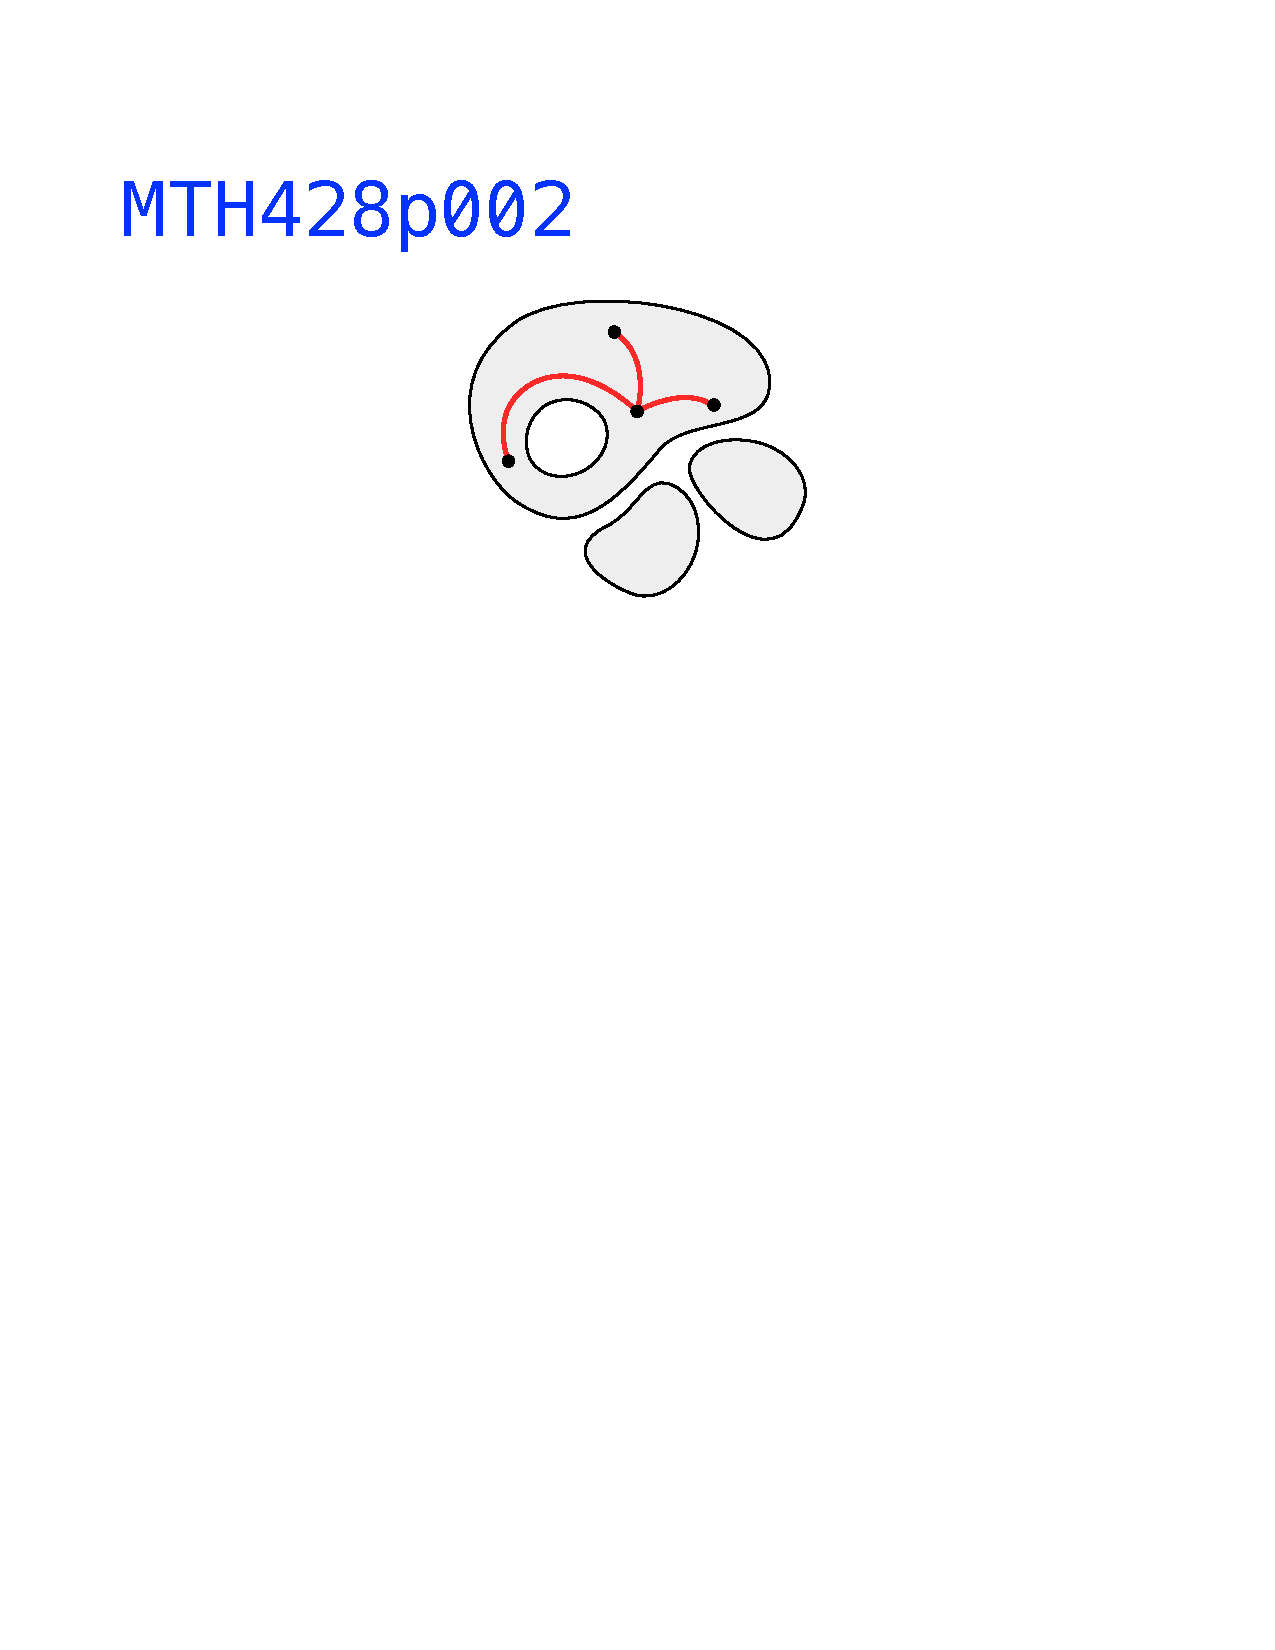
\includegraphics[width=\textwidth, trim=0mm 178mm 0mm 50mm, clip]{pictures/MTH428p002.pdf}}};

%%% COORDINATE GRID
%\draw[step=0.5, help lines] (0,0) to[grid with coordinates] (15,9);
%%% 

\node[anchor= base]  at (8.2 , 2.1){\small $x$};

\end{tikzpicture}
 
Denote this subspace by $[x]$.  Notice that for $x, x'\in X$ 
we have $[x] = [x']$ if and only if there is a path joining $x$ and $x'$. Let $\pi_{0}(X)$ denote the set 
whose elements are path connected components of the space $X$. Given a continuous function 
of topological spaces $f\colon X \to Y$ consider the function of sets 
$$f_{\ast}\colon \pi_{0}(X) \to \pi_{0}(Y)$$ 
given by $f_{\ast}([x]) = [f(x)]$. The function $f_{\ast}$ 
is well defined. Indeed, if  $x, x' \in X$ are points such that $[x] = [x']$ then there exists a path  
$\omega\colon [0, 1]\to X$ such that $\omega(0) =x$ and $\omega(1) = x'$. Then 
$f\omega\colon [0, 1]\to Y$ is a path joining $f(x)$ with $f(x')$ which shows that $[f(x)] = [f(x')]$. 
The assignments $X \mapsto \pi_{0}(X)$ and $f \mapsto f_{\ast}$ define a functor 
$\pi_{0}\colon \Top \to \Set$.
\end{example}

%---BBLANK
\begin{definition}
Let $\CC$ be a category. A morphism $f\colon c \to c'$ in $\CC$ is an \emph{isomorphism} if 
there exists a morphism $g\colon c'\to c$ such that $gf= \id_{c}$ and $fg = \id_{c'}$. In such case 
we say that $g$ is the \emph{inverse} of $f$ and we write $g = f^{-1}$. 

If there exists an isomorphism between  $c, c' \in \CC$ then we say that these objects are 
\emph{isomorphic} and we write $c\cong c'$.   
\end{definition}
%---EBLANK # \vskip 80mm

\begin{example}
A morphism  $f\colon X \to Y$ in $\Top$ is an isomorphism if and only if $f$ is a homeomorphism. 
\end{example}

\begin{example}
A morphism  $f\colon A \to B$ in $\Set$ is an isomorphism if and only if $f$ is a bijection of sets. 
\end{example}

\begin{example}
A morphism  $f\colon G \to H$ in $\Gr$ is an isomorphism if and only if $f$ is a group isomorphism. 
\end{example}

%---BBLANK
\begin{proposition}
\label{FUNCTOR PRES ISO PROP}
Let $F\colon \CC \to \DD$ be a functor. If $f\colon c \to c'$ is an isomorphism in $\CC$ then 
$F(f)\colon F(c) \to F(c')$
is an isomorphism in $\DD$ and $F(f)^{-1} = F(f^{-1})$.
\end{proposition}
%---EBLANK # \vskip 40mm

\begin{proof}
Let $f^{-1}\colon c' \to c$ be the inverse of $f$. We have 
$$F(f^{-1}) F(f) = F(f^{-1}f) = F(\id_{c}) = \id_{F(c)}$$
Similarly, using that $ff^{-1} = \id_{c'}$ we obtain  $F(f)F(f^{-1}) = \id_{F(c')}$. Thus $F(f^{-1})$
is the inverse of $F(f)$. 
\end{proof}

%---BBLANK
\begin{corollary}
Let $F\colon \CC \to \DD$ be a functor and $c, c'\in \CC$. If $F(c)\ncong F(c')$ then $c\ncong c'$.
\end{corollary}
%---EBLANK # \newpage

\begin{example}
Consider the functor $\pi_{0}\colon \Top \to \Set$ (\ref{PI ZERO FUNCTOR EXAMPLE}). 
In  $\Top$ take the spaces $\R$ and $\R\ssmin \{0\}$.  The space $\R$ has only one path connected 
component while $\R\ssmin \{0\}$ has two path connected components: $(-\infty, 0)$ and $(0, +\infty)$. 
It follows that  $\pi_{0}(\R)$ consists of one element while $\pi_{0}(\R \ssmin \{0\})$ is a set with two elements, 
so $\pi_{0}(\R)\ncong \pi_{0}(\R\ssmin \{0\})$ in $\Set$. This shows that $\R\ncong \R\ssmin \{0\}$ in 
$\Top$, i.e. that these two spaces are not homeomorphic. 
\end{example}


\begin{note}
For a general functor $F\colon \CC\to \DD$ and $c, c'\in \CC$ it may happen that $F(c)\cong F(c')$
even though $c\ncong c'$. Take for example the functor $\pi_{0}\colon \Top \to \Set$ and let $X = \{\ast\}$ be a 
space consisting of a single point. We have $\pi_{0}(X)\cong \pi_{0}(\R)$, since both $\pi_{0}(X)$
and $\pi_{0}(\R)$ are sets with only one element, but $X\ncong \R$. 
\end{note}

%%%%%%%%%%%%%%%%%%%%%%%%%%%%%%%
%  EXERCISES
%%%%%%%%%%%%%%%%%%%%%%%%%%%%%%%

\exercises


\begin{exercise}
Let $\CC$ be a category. An object $c\in \CC$ is initial in $\CC$
if for each object $d\in \CC$ there is exactly  one morphism $c\to d$.

a) Show that if $c$ is an initial object in $\CC$ and $c'\in \CC$ is an object 
isomorphic to $c$ then $c'$ is also an initial object. 

b) Show that if $c$ and $c'$ are objects of $\CC$ such that each of them is initial 
then $c\cong c'$. 
\end{exercise}



\begin{exercise}
Given  a morphism  $f\colon c \to c'$ and an object $d$ in a category $\CC$, consider the functions 
$$f_{\ast}\colon \Mor_{\CC}(d, c) \to \Mor_{\CC}(d, c') \ \ \ \ \ \text{and}  \ \ \ \ 
f^{\ast}\colon \Mor_{\CC}(c', d) \to \Mor_{\CC}(c, d)$$
given by $f_{\ast}(g) = f\circ g$  for $g \in  \Mor_{\CC}(d, c)$, 
and $f^{\ast}(h) = h\circ f$ for $h \in  \Mor_{\CC}(c', d)$. 

Show that  for a  morphism $f\colon c \to c'$  the following conditions are equivalent:
\benu
\item[1)] The morphism $f$ is is an isomorphism.
\item[2)] The function $f_{\ast}$ is a bijection for every $d\in \CC$.
\item[3)] The function $f^{\ast}$ is a bijection for every $d\in \CC$. 
\eenu
\end{exercise}


\begin{exercise}
Cosider a sequence of five morphisms in a category $\CC$:
$$
c_{0} \xrightarrow{f_{1}} 
c_{1} \xrightarrow{f_{2}} 
c_{2} \xrightarrow{f_{3}} 
c_{3} \xrightarrow{f_{4}} 
c_{4} \xrightarrow{f_{5}} 
c_{5}
$$
Assume that the composition of any three morphisms in this sequence $f_{3}\circ f_{2}\circ f_{1}$, 
$f_{4}\circ f_{3}\circ f_{2}$, and $f_{5}\circ f_{4}\circ f_{3}$ is an isomorphism. Show that 
$f_{i}$ is an isomorphism for $i=1,\dots, 5$.
\end{exercise}

\begin{exercise}
Find two different functors $F, F' \colon \Gr \to \Gr$ such that $F(G) = F'(G) = G$ for each group 
$G\in \Gr$.  
\end{exercise}





\begin{exercise}
\label{FULL FAITHFUL EXERCISE}
Let $\CC$, $\DD$ be categories. A functor $F\colon \CC \to \DD$ is called \emph{full} if for each 
$c, c'\in \CC$ the function 
$$F\colon \Mor_{\CC}(c, c') \to \Mor_{\DD}(F(c), F(c'))$$
is onto, and if is \emph{faithful} if for each $c, c'\in \CC$ this function is 1-1. 

a) Give an example of a functor $F\colon \Gr \to \Gr$ which is full but not faithful. 

b) Give an example of a functor $F'\colon \Gr \to \Gr$ which is faithful but not full. 

\end{exercise}


\begin{exercise}
Let $F\colon \CC\to \DD$ be a functor which is both full and faithful (Exercise \ref{FULL FAITHFUL EXERCISE}), 
and let $c, c' \in \CC$. Show that $c\cong c'$ if and only if $F(c)\cong F(c')$. 
\end{exercise}








\newpage
%%%%%%%%%%%%%%%%%%%%%%%%%%%%%%%
%%%%%%%%%%%%%%%%%%%%%%%%%%%%%%%
%%%
%%%  THE FUNDAMENTAL GROUP
%%%
%%%%%%%%%%%%%%%%%%%%%%%%%%%%%%%
%%%%%%%%%%%%%%%%%%%%%%%%%%%%%%%

%---BBLANK
\chapter[The Fundamental Group]{The Fundamental \\ Group}
%---EBLANK # \vskip -30mm

\chaptermark{The Fundamental Group}
\label{FUND GP CHAPTER}

\thispagestyle{firststyle}

%---BBLANK
\begin{definition} A \emph{pointed topological space} is a pair $(X, x_{0})$, where 
$X$ is a topological space and $x_{0}\in X$. We say that $x_{0}$ is the \emph{basepoint}
of $X$. Given two pointed spaces $(X, x_{0})$ and $(Y, y_{0})$ a \emph{basepoint preserving 
map} $f\colon (X, x_{0}) \to (Y, y_{0})$ is a continuous function $f\colon X \to Y$ such that $f(x_{0}) = y_{0}$. 
\end{definition}
%---EBLANK # \vskip 25mm


Let $\Top_{\ast}$ denote the category the objects of which are pointed spaces and morphisms 
are basepoint preserving maps. Our goal in this chapter will be to construct the 
\emph{fundamental group functor} 
$$\pi_{1}\colon \Top_{\ast} \to \Gr$$
That is, we will construct an assignment that associates to every pointed space $(X, x_{0})$
a group $\pi_{1}(X, x_{0})$ and to every basepoint preserving map $f\colon (X, x_{0}) \to (Y, y_{0})$ 
a group homomorphism $f_{\ast}\colon \pi_{1}(X, x_{0}) \to \pi_{1}(Y, y_{0})$ in a way that 
preserves  identity functions and compositions of functions.

Recall that a path in a space $X$ is a continuous function $\omega \colon [0, 1] \to X$. 

%---BBLANK
\begin{definition}
Let $\omega, \omega'\colon [0, 1]\to X$ be paths such that $\omega(0) = \omega'(0) = x_{0}$
and $\omega(1) = \omega'(1) = x_{1}$ for some $x_{0}, x_{1}\in X$. 
We say that the paths $\omega$ and $\omega'$ are 
\emph{path homotopic} if for every $t\in [0, 1]$ there exists a path 
$h_{t}\colon [0, 1] \to X$  such that:
\benu
\item[1)] $h_{t}(0) = x_{0}$, and $h_{t}(1) = x_{1}$ for all $t\in [0, 1]$
\item[2)] $h_{0} = \omega$,  and $h_{1} = \omega'$
\item[3)] the function $h\colon [0, 1]\times [0,1] \to X$ given by $h(s, t) = h_{t}(s)$
is continuous. 
\eenu
In this case we write $\omega \simeq \omega'$ and we say that $h$ is a
\emph{path homotopy} between $\omega$ and $\omega'$.  

\begin{tikzpicture}

\node[anchor=south west,inner sep=0] at (0,0) 
{{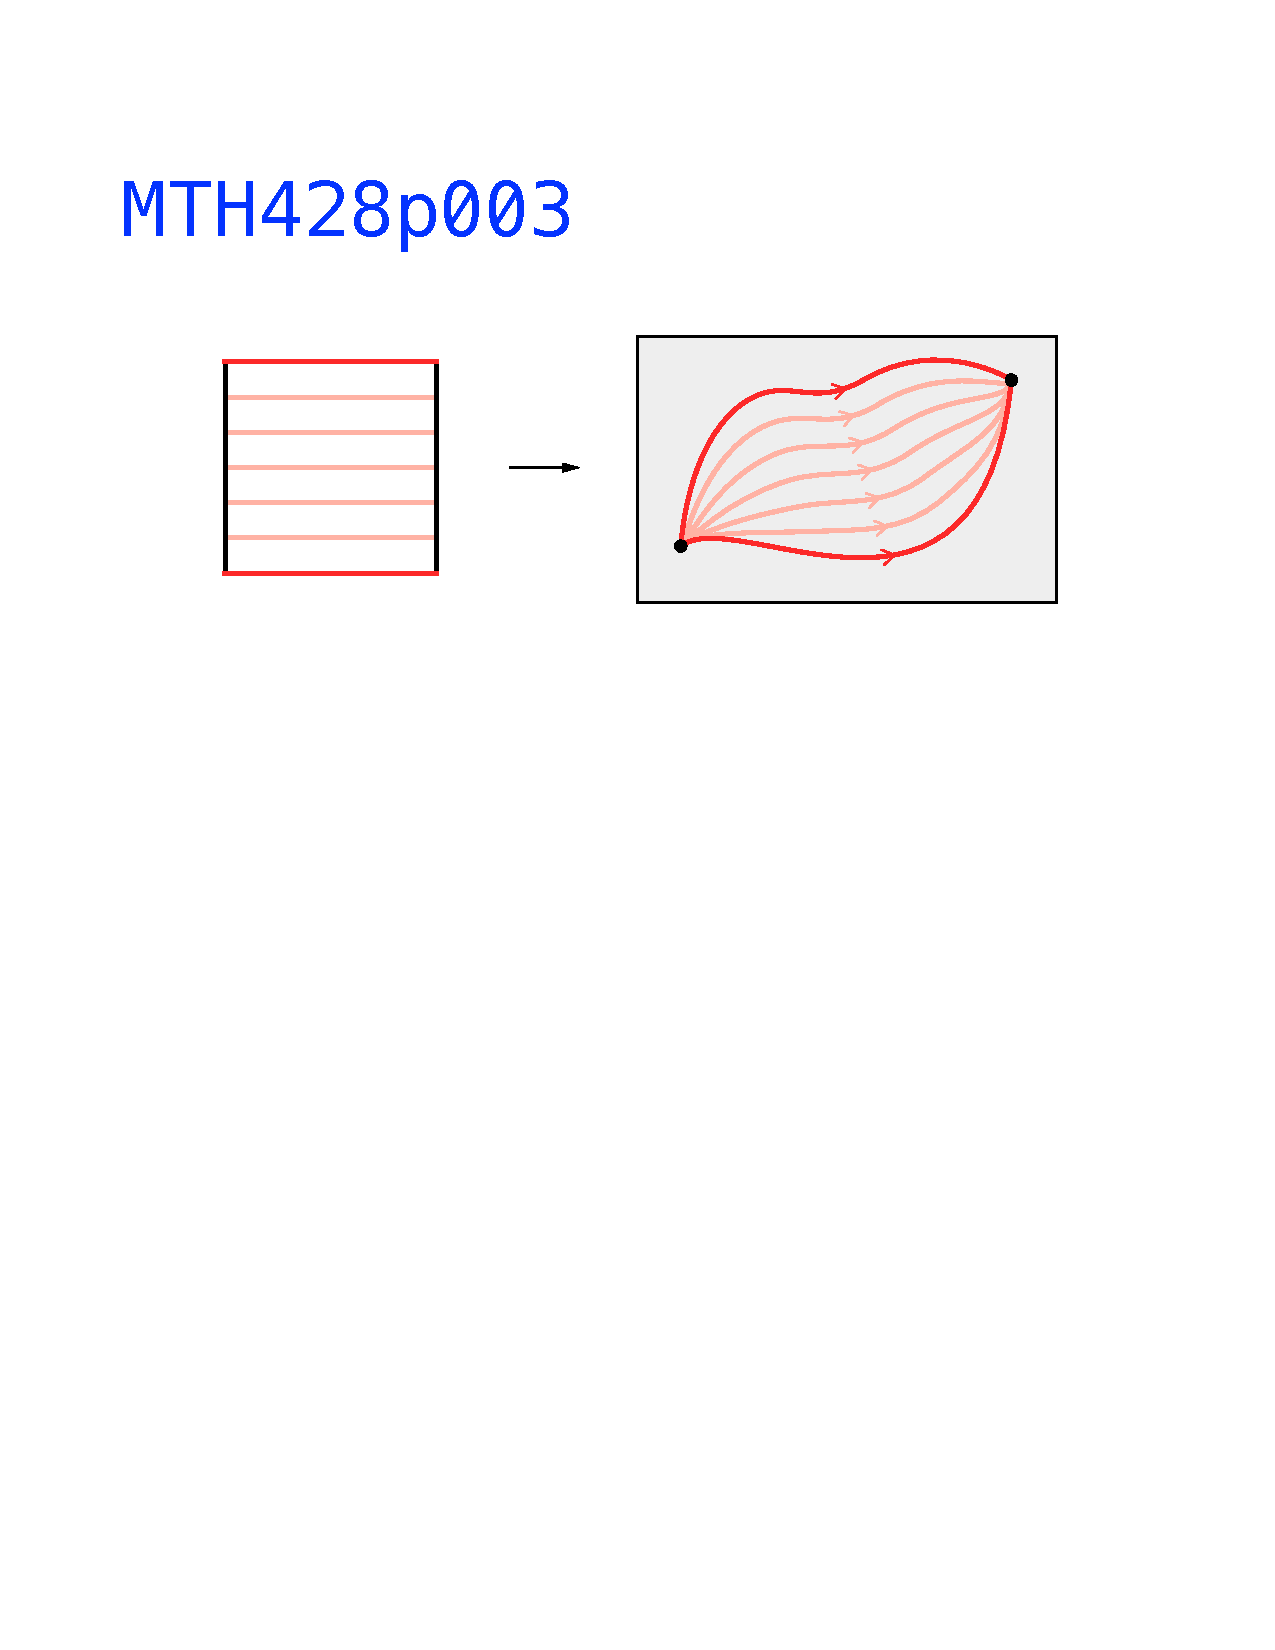
\includegraphics[width=\textwidth, trim=0mm 175mm 0mm 55mm, clip]{pictures/MTH428p003.pdf}}};

%%% COORDINATE GRID
%\draw[step=0.5, help lines] (0,0) to[grid with coordinates] (15,9);
%%% 

\node[anchor= base]  at (8.6 , 3.2){\small $X$};
\node[anchor= base]  at (8.7 , 0.55){\small $x_{0}$};
\node[anchor= base]  at (13.4 , 3.2){\small $x_{1}$};
\node[anchor= base]  at (10.78 , 3.15){\small \color{red} $\omega'$};
\node[anchor= base]  at (11.55 , 0.4){\small \color{red} $\omega$};
\node[anchor= base]  at (7.05 , 2.1){\small $h$};
\node[anchor= base]  at (2.6 , 1.85){\small $x_{0}$};
\node[anchor= base]  at (6.0 , 1.85){\small $x_{1}$};
\node[anchor= base]  at (4.3 , 3.5){\small \color{red} $\omega'$};
\node[anchor= base]  at (4.35 , 0.21){\small \color{red} $\omega$};
\end{tikzpicture}

\end{definition}
%---EBLANK # \newpage

Intuitively, path homotopy is a device for detecting holes in topological spaces. If $\omega$
and $\omega'$ are paths in $X$ with the same endpoints but such that $\omega\not\simeq \omega'$ then  
it indicates that there is a hole in $X$ that prevents us from deforming $\omega$ to 
$\omega'$:


\begin{equation*}
\begin{tikzpicture}[
    scale = 1.6,
    d0/.style = {line width = 1.6pt},
    d1/.style= {postaction={decorate}, line width = 1.6pt, decoration={markings, mark=at position 0.55 with {\arrow[rotate=3]{stealth}}}},
    d2/.style = {postaction={decorate}, line width = 1.6pt, decoration={markings, mark=at position 0.54 with {\arrow[rotate=-2]{stealth}}}}
]

\draw[fill = mygray1] (0,0) rectangle (3, 2.0);
\draw[thick, fill = white] (1.5, 1) circle (0.45);
\draw[d1, red]  (0.5,0.5) ..controls +(0.2, 1.2) and +(-0.9, 0.3)..  (2.5,1.5) node[pos = 0.45, anchor = south, yshift = 3pt] {\small $\omega$};
\draw[d2, myblue]  (0.5,0.5) ..controls +(1.4, -0.6) and +(-0.2, -0.6)..  (2.5,1.5) node[pos = 0.5, anchor = north, yshift = -2pt] {\small $\omega'$};
\filldraw (0.5,0.5) circle (0.05) node[anchor = north east, yshift = -2pt] {\small $x_{0}$};
\filldraw (2.5,1.5) circle (0.05) node[anchor = south west, yshift = 2pt] {\small $x_{1}$};
\node[anchor = north west] at (0, 2.0) {\small $X$};
\end{tikzpicture}
\end{equation*}

%---BBLANK # \ \vskip 60mm
\begin{lemma}
\label{PATH HOMOT EQUIV REL LEMMA}
Let $X$ be a space and let $x_{0}, x_{1}\in X$. 
Path homotopy defines an equivalence relation on the set of paths in $X$ that start at  $x_{0}$ and 
terminate at  $x_{1}$. 
 \end{lemma}

 
\begin{proof}
Exercise. 
\end{proof}
 %---EBLANK # \vskip 40mm

%---BBLANK
\begin{definition}
For a path $\omega$ we will denote by $[\omega]$ the equivalence class of $\omega$ taken with respect 
to  the equivalence relation given by path homotopy. We will say that $[\omega]$ is the \emph{homotopy class} of $\omega$.
\end{definition}
%---EBLANK # \newpage

\begin{notation}
Let $X$ be a space and let $x_{0}, x_{1}\in X$. By $\pi_{1}(X, x_{0}, x_{1})$ we will denote the set of
homotopy classes of paths that begin at $x_{0}$ and terminate at $x_{1}$.  If $x_{0} = x_{1}$ then 
we will write $\pi_{1}(X, x_{0})$ instead of $\pi_{1}(X, x_{0}, x_{0})$. Notice that elements 
of $\pi_{1}(X, x_{0})$ are homotopy classes $[\omega]$ where $\omega$ is a path such that 
$\omega(0) = \omega(1) = x_{0}$. We call such $\omega$ a \emph{loop} based at $x_{0}$. 
\end{notation}


%---BBLANK
\begin{definition}
Let $\omega, \tau \colon [0, 1] \to X$ be paths such that $\omega(1) = \tau(0)$. 
The \emph{concatenation} of $\omega$ and $\tau$ is the path 
$\omega \ast \tau\colon [0, 1]\to X$ given by 
$$
(\omega\ast \tau)(s) = 
\begin{cases}
\omega(2s) & \text{ for } s\in [0, \frac{1}{2}] \\
\tau(2s -1) & \text{ for } s\in [\frac{1}{2}, 1] \\
\end{cases}
$$ 

\begin{equation*}
\begin{tikzpicture}[
    scale = 1,
    d0/.style = {line width = 1.6pt},
    d1/.style= {postaction={decorate}, line width = 1.6pt, decoration={markings, mark=at position 0.55 with {\arrow[rotate=-2]{stealth}}}},
    d2/.style = {postaction={decorate}, line width = 1.6pt, decoration={markings, mark=at position 0.54 with {\arrow[rotate=4]{stealth}}}}
]

\draw[d0, red] (0,0) -- node[anchor=south, yshift = 2pt] {\small $\omega$} (1.5, 0); 
\draw[d0, myblue] (1.5,0) --  node[anchor=south, yshift = 2pt] {\small $\tau$} (3, 0); 
\filldraw (0,0) circle (0.08) node[anchor = north, yshift = -2pt] {\small $0$};
\filldraw (1.5,0) circle (0.08) node[anchor = north, yshift = -2pt] {\small $\frac{1}{2}$};
\filldraw (3,0) circle (0.08) node[anchor = north, yshift = -2pt] {\small $1$};

\draw[thick, ->, >=latex] (3.7, 0) -- node[anchor= south] {\small $\omega\ast \tau$}(4.9, 0);


\begin{scope}[xshift = 8pt]
\draw[fill=mygray1] (5.2, -1.25) rectangle (9.5, 1.5);
\node[anchor = north west] at (5.2, 1.5) {\small $X$};

\begin{scope}[yshift = 7pt, xshift = 5pt]
\draw[d2, red] (5.75, - 0.75) ..controls +(0,1) and +(-0.5,0).. node[pos = 0.5, anchor= north west, xshift = -3pt, yshift = -1pt] {\small $\omega$} (7.5,0.4);
\draw[d1, myblue] (7.5,0.4) ..controls +(0,-0.5) and +(-0.5,0).. node[pos = 0.5, anchor= north west, xshift = 1pt, yshift = 11pt] {\small $\tau$} (8.5, -0.75);
\filldraw (5.75, - 0.75) circle (0.08);
\filldraw (7.5,0.4) circle (0.08);
\filldraw (8.5, -0.75) circle (0.08);
\end{scope}
\end{scope}

\end{tikzpicture}
\end{equation*}

\end{definition}
%---EBLANK # \vskip 10mm

%---BBLANK
\begin{proposition}
\label{HOMOT INV OF CONCATENATION PROP}
Let $\omega$ ,$\tau$ be paths in $X$ such that $\omega(1) = \tau(0)$. If $\omega'$, $\tau'$
are paths such that $\omega\simeq \omega' $ and $\tau \simeq \tau' $
then $\omega\ast \tau \simeq \omega'\ast\tau' $. 
\end{proposition}
%---EBLANK # \newpage

\begin{proof}
Let $h^{\omega}\colon [0, 1]\times [0, 1] \to X$ be a path homotopy between $\omega$ and $\omega'$
and $h^{\tau} \colon [0, 1]\times [0, 1] \to X$ be a path homotopy between $\tau$ and $\tau'$. Define 
$h\colon [0, 1]\times [0, 1] \to X$ by 
$$
h(s, t) = 
\begin{cases}
h^{\omega}(2s, t) & \text{ for } s\in [0, \frac{1}{2}] \\
h^{\tau}(2s -1, t)   &  \text{ for } s\in [\frac{1}{2}, 1] \\
\end{cases}
$$
The map $h$ is a path homotopy between $\omega\ast\tau$ and $\omega'\ast \tau'$. 


\begin{equation*}
\begin{tikzpicture}[scale = 0.9]
\draw[line width = 1.8pt] (0,0) rectangle (3,3);
\draw (1.5, 0) -- (1.5, 3.0);
\draw[red, line width = 1.8pt, cap=rect] (0, 0)  -- node[anchor = north] {\small \color{red} $\omega$}(1.5, 0);
\draw[myblue, line width = 1.8pt] (1.5, 0) -- node[anchor = north] {\small \color{myblue} $\tau$}(3, 0);
\draw[myblue, line width = 1.8pt, cap=rect] (2, 0) -- (3, 0);
\draw[red, line width = 1.8pt, cap=rect] (0, 3)  --  node[anchor = south] {\small \color{red} $\omega'$} (1.5, 3);
\draw[myblue, line width = 1.8pt] (1.5, 3) -- node[anchor = south] {\small \color{myblue} $\tau'$} (3, 3);
\draw[myblue, line width = 1.8pt, cap=rect] (2, 3) -- (3, 3);
\draw[draw opacity = 0] (0,0) rectangle node {\small $h^{\omega}$}(1.5, 3);
\draw[draw opacity = 0] (1.5,0) rectangle node {\small $h^{\tau}$}(3, 3);
\end{tikzpicture}
\end{equation*}
\end{proof}




Notice that by Proposition \ref{HOMOT INV OF CONCATENATION PROP} the homotopy 
class of $\omega\ast \tau$ depends only on the homotopy classes of $\omega$ and $\tau$. Therefore 
for any $x_{0}, x_{1}, x_{2}\in X$ we obtain a well defined function 
$$\mu\colon \pi_{1}(X, x_{0}, x_{1}) \times \pi_{1}(X, x_{1}, x_{2}) \to \pi_{1}(X, x_{0}, x_{2})$$
where $\mu([\omega], [\tau]) = [\omega\ast \tau]$. To simplify notation we will  write 
$[\omega]\cdot [\tau]$ instead of $\mu([\omega], [\tau])$. 
In the case when $x_{0} = x_{1} = x_{2}$ this gives a multiplication on the set $\pi_{1}(X, x_{0})$:
$$\pi_{1}(X, x_{0})\times \pi_{1}(X, x_{0}) \to \pi_{1}(X, x_{0}), \ \ \ [\omega]\cdot [\tau] = [\omega\ast \tau]$$
Our next goal will be to show that the set $\pi_{1}(X, x_{0})$ taken with this multiplication is a group. 

%---BBLANK
\begin{lemma}
\label{PATH CONCAT HOMOT ASSOC LEMMA}
If $\omega, \tau, \sigma$ are paths in a space $X$ such that $\omega(1) = \tau(0)$ 
and $\tau(1) = \sigma(0)$ then 
$$([\omega]\cdot[\tau])\cdot[\sigma] =  [\omega]\cdot([\tau]\cdot[\sigma])$$


\begin{equation*}
\begin{tikzpicture}
\draw[fill = mygray1] (0,0) rectangle (5, 2.5);

\draw[line width = 1.4pt, red, postaction={decorate}, decoration={markings, mark= at position 0.55 with {\arrow[rotate= 4]{stealth}}}] (0.75,0.75) ..controls +(0,0.5) and +(-0.7,0).. node[pos = 0.5, anchor= north west, xshift = -1pt, yshift = 2pt] {\small $\omega$} (2,1.75);
\draw[line width = 1.4pt, red, postaction={decorate}, decoration={markings, mark= at position 0.55 with 
{\arrow[rotate= -7]{stealth}}}] 
(2,1.75) ..controls +(0,-0.8) and +(-0.2,0).. node[pos = 0.5, anchor= south west, xshift = -4pt, yshift = 0pt] {\small $\tau$} (3, 0.75);
\draw[line width = 1.4pt, red, postaction={decorate}, decoration={markings, mark= at position 0.55 with {\arrow[rotate = 6]{stealth}}}] (3, 0.75) ..controls +(0, 0.7) and +(-0.2, 0).. node[pos = 0.4, anchor= north west, xshift = -2pt, yshift = 2pt] {\small $\sigma$} (4.25, 1.75);

\filldraw (0.75,0.75) circle (0.07);
\filldraw (2,1.75) circle (0.07);
\filldraw (3, 0.75) circle (0.07);
\filldraw (4.25, 1.75) circle (0.07);

\node[anchor = north west, xshift = 2pt, yshift = - 3pt] at (0, 2.5) {\small $X$};

\end{tikzpicture}
\end{equation*}

\end{lemma}
%---EBLANK # \newpage



\begin{proof}

We have: 
$$([\omega]\cdot[\tau])\cdot[\sigma]  = [\omega\ast\tau]\cdot[\sigma] = 
[(\omega\ast\tau)\ast \sigma]$$


\begin{equation*}
\begin{tikzpicture}[scale = 1.2]
\draw[line width = 1.8pt, red] (0,0) -- node[anchor = south, outer sep = 4pt] {\small $\color{red}\omega$} (1,0);
\draw[line width = 1.8pt, red] (1,0) -- node[anchor = south, outer sep = 4pt] {\small $\color{red}\tau$} (2,0);
\draw[line width = 1.8pt, red] (2,0) -- node[anchor = south, outer sep = 4pt] {\small $\color{red}\sigma$} (4,0);
\draw[fill = black] (0,0) node[anchor = north, outer sep = 4pt] {\small $0$} circle  (0.07);
\draw[fill = black] (4,0) node[anchor = north, outer sep = 4pt] {\small $1$} circle (0.07);
\draw[fill = black] (2,0) node[anchor = north, outer sep = 4pt] {\small $\frac{1}{2}$} circle (0.07);
\draw[fill = black] (1,0) node[anchor = north, outer sep = 4pt] {\small $\frac{1}{4}$} circle (0.07);
\end{tikzpicture}
\end{equation*}

Similarly: 
$$ [\omega]\cdot([\tau]\cdot[\sigma])  = [\omega]\cdot [\tau \ast \sigma] = 
[\omega\ast (\tau \ast \sigma)]$$

\begin{equation*}
\begin{tikzpicture}[scale = 1.2]
\draw[line width = 1.8pt, red] (0,0) -- node[anchor = south, outer sep = 4pt] {\small $\color{red}\omega$} (2,0);
\draw[line width = 1.8pt, red] (2,0) -- node[anchor = south, outer sep = 4pt] {\small $\color{red}\tau$} (3,0);
\draw[line width = 1.8pt, red] (3,0) -- node[anchor = south, outer sep = 4pt] {\small $\color{red}\sigma$} (4,0);
\draw[fill = black] (0,0) node[anchor = north, outer sep = 4pt] {\small $0$} circle  (0.07);
\draw[fill = black] (4,0) node[anchor = north, outer sep = 4pt] {\small $1$} circle (0.07);
\draw[fill = black] (2,0) node[anchor = north, outer sep = 4pt] {\small $\frac{1}{2}$} circle (0.07);
\draw[fill = black] (3,0) node[anchor = north, outer sep = 4pt] {\small $\frac{3}{4}$} circle (0.07);
\end{tikzpicture}
\end{equation*}


We need to show that $(\omega\ast \tau) \ast \sigma \simeq \omega\ast (\tau \ast \sigma)$. 
Graphically a homotopy $h\colon [0, 1]\times [0, 1]\to X$  between these  paths can be represented 
as follows:


\begin{equation*}
\begin{tikzpicture}[scale = 0.7]
\draw[line width = 1.6 pt, mypink] (0,2) -- (4,2);
\draw[line width = 1.6 pt] (0,0) rectangle (4,4);
\draw[line width = 1.6 pt, cap = rect, red] (0,0) -- (4,0) (0,4) -- (4,4); 
\draw[thick] (2,4) -- (1,0) (3, 4)--(2, 0);
\draw[fill = black] (0, 0) node[anchor=north, yshift = -2pt] {\small $0$} circle (0.09);
\draw[fill = black] (1, 0) node[anchor=north, yshift = -2pt] {\small $\frac{1}{4}$} circle (0.09);
\draw[fill = black] (2, 0) node[anchor=north, yshift = -2pt] {\small $\frac{1}{2}$} circle (0.09);
\draw[fill = black] (4, 0) node[anchor=north, yshift = -2pt] {\small $1$} circle (0.09);
\draw[fill = black] (0, 4) node[anchor=south, yshift = 2pt] {\small $0$} circle (0.09);
\draw[fill = black] (2, 4) node[anchor=south, yshift = 2pt] {\small $\frac{1}{2}$} circle (0.09);
\draw[fill = black] (3, 4) node[anchor=south, yshift = 2pt] {\small $\frac{3}{4}$} circle (0.09);
\draw[fill = black] (4, 4) node[anchor=south, yshift = 2pt] {\small $1$} circle (0.09);
\node[red, anchor = south] at (0.8, 2) {\small $\omega$};
\node[red, anchor = south] at (2, 2) {\small $\tau$};
\node[red, anchor = south] at (3.2, 2) {\small $\sigma$};
\end{tikzpicture}
\end{equation*}


More precisely, $h$ is given by the following formula:

$$
h(s, t) = 
\begin{cases}
\omega \left(\frac{4s}{t+1} \right) & \text{ for } s\in [0, \frac{t+1}{4}] \\[2mm]
\tau(4s -t -1) & \text{ for } s\in [\frac{t+1}{4}, \frac{t+2}{4}] \\[2mm]
\sigma \left( \frac{4s-t-2}{2-t} \right) & \text{ for } s\in [\frac{t+2}{4}, 1] \\
\end{cases}
$$
\end{proof}

%---BBLANK
\begin{lemma}
\label{CONSTANT PATH CONCAT LEMMA}
Let $X$ be a space, and let $x_{0}\in X$. Let $c_{x_{0}}\colon [0, 1]\to X$ denote the constant path 
at the point $x_{0}$: $c_{x_{0}}(s) = x_{0}$ for all $t\in [0, 1]$. If $\omega$ is a path in $X$ such that 
$\omega(0) = x_{0}$ then $[c_{x_{0}}]\cdot [\omega] = [\omega]$.
Also, if $\tau$ is a path such that $\tau(1) = x_{0}$ then 
 $[\tau] \cdot [c_{x_{0}}] = [\tau]$.
\end{lemma}
%---EBLANK # \vskip 80mm

\begin{proof}
To obtain the first equality we need to check that $c_{x_{0}}\ast \omega \simeq \omega$. 
A homotopy between these paths can be represented as follows: 

\begin{equation*}
\begin{tikzpicture}[scale = 0.7]
\draw[line width = 1.6 pt, mypink] (0,2) -- (4,2);
\draw[line width = 1.6 pt] (0,0) rectangle (4,4);
\draw[line width = 1.6 pt, cap = rect, red] (0,0) -- (4,0) (0,4) -- (4,4); 
\draw[thick] (0,4) -- (2,0);
\draw[fill = black] (0, 0) node[anchor=north, yshift = -2pt] {\small $0$} circle (0.09);
\draw[fill = black] (2, 0) node[anchor=north, yshift = -2pt] {\small $\frac{1}{2}$} circle (0.09);
\draw[fill = black] (4, 0) node[anchor=north, yshift = -2pt] {\small $1$} circle (0.09);
\draw[fill = black] (0, 4) node[anchor=south, yshift = 2pt] {\small $0$} circle (0.09);
\draw[fill = black] (4, 4) node[anchor=south, yshift = 2pt] {\small $1$} circle (0.09);
\node[red, anchor = north, yshift = -1pt] at (0.6, 2) {\small $c_{x_{0}}$};
\node[red, anchor = north, yshift = -1pt] at (2, 2) {\small $\omega$};
\end{tikzpicture}
\end{equation*}

The second equality comes from a homotopy $\tau\ast c_{x_{0}}\simeq \tau$ that can be obtained
in a similar way. 

\end{proof}

Let $\omega \colon [0, 1] \to X$ be a path. By
$\xov{\omega}$ we will denote the path given by $\xov{\omega}(s) = \omega(1-s)$ for $s\in [0,1]$. 
In other words $\xov\omega$ is obtained by reversing the orientation of $\omega$::

\begin{equation*}
\begin{tikzpicture}
\draw[fill = mygray1] (0, 0.2) rectangle (4, 2.2);




% Draw curved path
\draw[myblue, line width = 1.6pt]
(0.5, 0.5) 
.. controls +(0.5, 1.3) and +(-0.5, 1.3) ..
(3.5, 0.5)  {\foreach \i in {1,...,40} {  coordinate[pos= \i/40] (p\i) } };;

\draw[->, >=angle 60, mygray1, very thick, rotate around={12:($(p15)!1.5pt!90:(p16)$)}] 
($($(p15)!1.5pt!90:(p16)$)!0.25!($(p16)!1.5pt!90:(p17)$)$) -- +(-0.01, 0); 
\draw[->, >=angle 60, mygray1, very thick, rotate around={12:($(p15)!1.5pt!90:(p16)$)}] 
($($(p15)!1.5pt!90:(p16)$)!0.25!($(p14)!1.5pt!90:(p15)$)$) -- +(-0.06, 0); 




% Draw parallel curve
% (note that first and last points are specified out of the loop)
\draw[red, line width = 1.6pt] ($(0.5, 0.5)!1.5pt!90:(p2)$) 
{ \foreach \i [count=\j from 2] in {1,...,39} {-- ($(p\i)!1.5pt!90:(p\j)$) } }
 -- ($(p40)!1.5pt!-90:(p39)$);
 
 

 \draw[->, >=angle 60, mygray1,very thick, rotate around={-12:(p3)}] ($(p25)!0.25!(p26)$) -- +(0.07, 0); 
  \draw[->, >=angle 60, mygray1,very thick, rotate around={-12:(p3)}] ($(p25)!0.25!(p24)$) -- +(0.01, 0); 
 
 \begin{scope}
 \clip (p25) circle (0.5); 
 \draw[myblue, line width = 1.6pt]
(0.5, 0.5) 
.. controls +(0.5, 1.3) and +(-0.5, 1.3) ..
(3.5, 0.5); 
 \end{scope}
 
 
 \draw[mygray1, line width = 0.4pt] ($(0.5, 0.5)!0.75pt!90:(p2)$) 
{ \foreach \i [count=\j from 2] in {1,...,39} {-- ($(p\i)!0.75pt!90:(p\j)$) } }
 -- ($(p40)!0.75pt!-90:(p39)$);


\draw[->, >=angle 60, myblue, very thick, rotate around={-12:(p25)}] (p25) -- +(0.035, 0); 
\draw[->, >=angle 60, red, very thick, rotate around={12:($(p15)!1.5pt!90:(p16)$)}] ($(p15)!1.5pt!90:(p16)$) -- +(-0.035, 0); 

\fill[xshift = -0.75pt] (0.5, 0.5) circle (0.07);
\fill[xshift = 0.75pt] (3.5, 0.5) circle (0.07);
\node at (0.3, 1.9) {\small $X$};
\node at (2, 1.2) {\small \color{myblue} $\omega$};
\node at (2, 1.8) {\small \color{red} $\xov\omega$};
\end{tikzpicture}
\end{equation*}


 We will say that $\xov{\omega}$ is the \emph{inverse} 
of $\omega$. This name is justified by the following fact:

%---BBLANK
\begin{lemma}
\label{INVERSE PATH CONCAT LEMMA}
Let $\omega$ be a path in a space $X$ such that $\omega(0) = x_{0}$ and $\omega(1) = x_{1}$. We have:
$$[\omega]\cdot[\xov{\omega}] = [c_{x_{0}}], \ \ \ \ \ [\xov{\omega}]\cdot[\omega] = [c_{x_{1}}]$$
\end{lemma}
%---EBLANK # \newpage


\begin{proof}
Intuitively, a homotopy $h$ between  $c_{x_{0}}$  and $\omega\ast\xov{\omega}$ can be obtained 
by taking $h_{t}$ to be the path that goes from $x_{0}$ to the point $\omega(t) = \xov{\omega}(1-t)$ 
along $\omega$, and the follows $\xov{\omega}$ back to $x_{0}$. Formally, we can define $h$ as follows:
$$h(s, t)= 
\begin{cases}
\omega(2st) & \text{ for } s\in [0, \frac{1}{2}] \\
\omega((2-2s)t) & \text{ for } s\in [\frac{1}{2}, 1] \\
\end{cases}
$$
\end{proof}


%---BBLANK
\begin{proposition}
Let $X$ be a topological space and let $x_{0}\in X$. The set $\pi_{1}(X, x_{0})$ taken with the multiplication 
given by 
$$[\omega]\cdot [\tau]  = [\omega\ast\tau]$$
for $[\omega], [\tau]\in \pi_{1}(X, x_{0})$ is a group. 
The trivial element in this group is the homotopy class of the constant path $[c_{x_{0}}]$, and 
for $[\omega]\in \pi_{1}(X, x_{0})$ we have $[\omega]^{-1} = [\xov{\omega}]$. 
\end{proposition}
%---EBLANK # \vskip 60mm

\begin{proof}
The multiplication is associative by Lemma \ref{PATH CONCAT HOMOT ASSOC LEMMA}. 
The element $[c_{x_{0}}]$ is trivial with respect to this multiplication by 
Lemma \ref{CONSTANT PATH CONCAT LEMMA}, and $[\xov{\omega}]$ is the multiplicative inverse
of $[\omega]$ by Lemma \ref{INVERSE PATH CONCAT LEMMA}.  
\end{proof}


%---BBLANK
\begin{definition}
Let $(X, x_{0})$ be a pointed space. The group $\pi_{1}(X, x_{0})$ is called the \emph{fundamental group}
of $(X, x_{0})$. 
\end{definition}
%---EBLANK # \newpage


%---BBLANK
\begin{lemma}
\label{PATH HOMOTOPY IMAGE LEMMA}
Let $f\colon (X, x_{0}) \to (Y, y_{0})$ be a map of pointed spaces. If $\omega\colon [0, 1]\to X$
is a loop in $X$ based at $x_{0}$ then $f\circ \omega\colon [0, 1]\to Y$ is a loop in $Y$ based at $y_{0}$. 
Moreover, if $\omega'$ is another  loop in $X$ based at $x_{0}$ such that $\omega\simeq \omega'$ then 
$f\circ \omega\simeq f\circ \omega'$. 
\end{lemma} 
%---EBLANK # \vskip 40mm

\begin{proof}
If $h\colon [0,1]\times [0, 1] \to X$ is a homotopy between $\omega$ and $\omega'$ then 
$f\circ h\colon [0, 1]\times [0, 1]\to Y$ gives a homotopy between $f\omega$ and $f\omega'$. 
\end{proof}

By Lemma \ref{PATH HOMOTOPY IMAGE LEMMA}  each map of pointed spaces 
$f\colon (X, x_{0}) \to (Y, y_{0})$ defines a function 
$$f_{\ast}\colon \pi_{1}(X, x_{0}) \to \pi_{1}(Y, y_{0})$$
given by $f_{\ast}([\omega]) = [f\circ \omega]$. In addition we have:

%---BBLANK 
\begin{proposition}
If $f\colon (X, x_{0})\to (Y, y_{0})$ is a map of pointed spaces then the function 
$f_{\ast}\colon \pi_{1}(X, x_{0}) \to \pi_{1}(Y, y_{0})$ is a group homomorphism. 
\end{proposition}
%---EBLANK # \vskip 50mm


\begin{proof}
First, notice that $f\circ c_{x_{0}} = c_{y_{0}}$, so $f_{\ast}([c_{x_{0}}]) = [c_{y_{0}}]$. 
Also, if $\omega$, $\tau$ are loops in $X$ then 
$f\circ (\omega\ast\tau) = (f\circ\omega)\ast (f\circ \tau)$. This gives:
$$f_{\ast}([\omega]\cdot [\tau]) = [f\circ (\omega\ast\tau)] =  [(f\circ\omega)\ast (f\circ \tau)]
= [f\circ\omega]\cdot [f\circ\tau] = f_{\ast}([\omega])\cdot f_{\ast}([\tau])$$
\end{proof}

%---BBLANK 
\begin{corollary}
The assignments $(X, x_{0})\mapsto \pi_{1}(X, x_{0})$ and $f\mapsto f_{\ast}$ define a functor 
$$\pi_{1}\colon\Top_{\ast} \to \Gr$$
\end{corollary}
%---EBLANK # \vskip 40mm

\begin{proof}
We need to check that 
\benu
\item[1)] if $\id \colon (X, x_{0}) \to (X, x_{0})$ is the identity map, then 
$\id_{\ast}\colon \pi_{1}(X, x_{0}) \to \pi_{1}(X, x_{0})$
is the identify homomorphism;
\item[2)] if $f\colon (X, x_{0}) \to (Y, y_{0})$ and $g\colon (Y, y_{0}) \to (Z, z_{0})$ are 
maps of pointed spaces then $(g\circ f)_{\ast} = g_{\ast}\circ f_{\ast}$. 
\eenu
Property 1) holds since $\id_{\ast}([\omega]) = [\id \circ \omega] = [\omega]$. Similarly, 
property 2) holds since 
$$(g\circ f)_{\ast}[\omega] = [g\circ f \circ \omega] = g_{\ast}([f\circ \omega]) = g_{\ast}(f_{\ast}([\omega]))
= g_{\ast}\circ f_{\ast}([\omega])$$ 
\end{proof}

Notice that an isomorphism in $\Top_{\ast}$ is a homeomorphism that preserves basepoints. 
As a consequence of Proposition \ref{FUNCTOR PRES ISO PROP} we obtain:

%---BBLANK 
\begin{corollary}
If $(X, x_{0}), (Y, y_{0})$ are pointed spaces and $f\colon X \to Y$ is a homeomorphism such that 
$f(x_{0}) = y_{0}$, then $f_{\ast}\colon \pi_{1}(X, x_{0})\to \pi_{1}(Y, y_{0})$ is an isomorphism. 
\end{corollary}
%---EBLANK # \newpage


\begin{note}
\label{HOMEO FUND GP NOTE}
If $f\colon X \to Y$ is any homeomorphism of topological spaces and $x_{0}\in X$ then 
we  get a homeomorphism of pointed spaces $f\colon (X, x_{0}) \to (Y, f(x_{0}))$, which gives an 
isomorphism $f_{\ast}\colon \pi_{1}(X, x_{0})\to \pi_{1}(Y, f(x_{0}))$. 
\end{note}

%---BBLANK 
\begin{note}
\label{PI1THROUGHS1 NOTE}
%---EBLANK  # Alternative construction of the fundamental group. \end{note} \newpage
In some settings it is convenient to use a somewhat different construction of the fundamental group
than the one described above. Recall the every element of $\pi_{1}(X, x_{0})$ can be represented by 
a function $\omega \colon [0, 1] \to X$ that satisfies $\omega(0) = \omega(1) = x_{0}$.  Such function uniquely 
determines a map $[0, 1]/{\sim} \to X$ from the quotient space $[0, 1]/{\sim}$ where 
$\sim$ is the equivalence relation identifying the endpoints of the interval: $0\sim 1$. 
The  space $[0, 1]/{\sim}$ is homeomorphic to the circle $S^{1}$. Under such homeomorphism the point 
$[0] \in [0, 1]/{\sim}$ is mapped to some point $s_{0}\in S^{1}$ that we can consider as a basepoint of 
$S^{1}$. As a consequence we obtain a bijection between two sets of maps:
$$
\begin{pmatrix}
\text{maps $\omega \colon [0, 1] \to X$} \\[1mm]
\text{with $\omega(0) = \omega(1) = x_{0}$} \\
\end{pmatrix}
\cong 
\begin{pmatrix}
\text{basepoint preserving maps} \\[1mm]
\text{$\omega \colon (S^{1}, s_{0}) \to (X, x_{0})$} \\
\end{pmatrix}
$$
Next, given two  maps $\omega, \tau\colon (S^{1}, s_{0}) \to (X, x_{0})$ 
we will say that $\omega$ and $\tau$ are homotopic if there is a continuous function 
$h\colon S^{1}\times [0, 1] \to X$ such that $h(s, 0) = \omega(s)$, $h(s, 1) = \tau(s)$ for all $s\in S^{1}$
and $h(s_{0}, t) = x_{0}$ for all $t\in [0, 1]$. The above bijection maps homotopic 
functions on one side to homotopic functions on the other side, so we obtain a bijection of sets:
$$
\begin{pmatrix}
\text{elements} \\[1mm]
\text{of the group} \\[1mm]
\text{$\pi_{1}(X, x_{0})$} \\
\end{pmatrix}
=
\begin{pmatrix}
\text{homotopy classes} \\[1mm]
\text{of maps $\omega \colon [0, 1] \to X$} \\[1mm]
\text{with $\omega(0) = \omega(1) = x_{0}$} \\
\end{pmatrix}
\cong 
\begin{pmatrix}
\text{homotopy classes } \\[1mm]
\text{of basepoint preserving maps} \\[1mm]
\text{$\omega \colon (S^{1}, s_{0}) \to (X, x_{0})$} \\
\end{pmatrix}
$$
In effect we can think of elements $\pi_{1}(X, x_{0})$ as homotopy classes of basepoint preserving 
maps $(S^{1}, s_{0})\to (X, x_{0})$. Using this interpretation the trivial element in $\pi_{1}(X, x_{0})$ is given by 
the homotopy class of the constant map $S^{1} \to X$. Multiplication in $\pi_{1}(X, x_{0})$ can be described as follows. Let $S^{1}\vee S^{1}$ denote the 
space obtained by taking two copies of $S^{1}$ and identifying a basepoint of one copy with 
the basepoint of the other copy:

\begin{equation*}
\begin{tikzpicture}[scale = 0.66]
\draw[line width = 1.6pt] (0,0) circle (1);
\draw[line width = 1.6pt] (0,2) circle (1);
\draw[fill = black] (0,1) circle (0.12);
\end{tikzpicture}
\end{equation*}

The \emph{pinch map} is a function $p\colon S^{1}\to S^{1}\vee S^{1}$ that wraps half of the circle 
around one copy of $S^{1}$ and the other half around the other copy:

\begin{equation*}
\begin{tikzpicture}[
    scale = 0.66,
    d0/.style = {line width = 1.6pt},
    d1/.style= {postaction={decorate}, line width = 1.6pt, decoration={markings, mark=at position 0.55 with {\arrow{stealth}}}},
    d2/.style = {postaction={decorate}, line width = 1.6pt, decoration={markings, mark=at position 0.54 with {\arrow[rotate=-9]{stealth}}}},
]

\begin{scope}
\draw[d2, red] (1,0) arc (0:180:1);
\draw[d2, myblue] (-1,0) arc (180:360:1);
\draw[fill = black] (-1,0) circle (0.12);
\draw[fill = black] (1,0) circle (0.12);
\end{scope}

\begin{scope}[xshift = 21mm]
\draw[thick, ->, >=latex] (0,0) -- node[anchor=south] {\small $p$} (1.5,0);
\end{scope}


\begin{scope}[xshift = 55 mm]
\draw[opacity = 0] (0 , -2.2) -- (0, 2.2); % dummy so that arrow on circle show
\draw[d2, red] (0,0) arc (-90:270:1);
\draw[d2, myblue] (0,0) arc (90:450:1);
\draw[fill = black] (0,0) circle (0.12);
\end{scope}

\end{tikzpicture}
\end{equation*}

Given  two functions $\omega, \tau \colon (S^{1}, s_{0}) \to (X, x_{0})$  define 
$\omega\vee \tau \colon S^{1}\vee S^{1} \to X$ to be the function
that maps one copy of $S^{1}$ by $\omega$ and the other by $\tau$:

\begin{equation*}
\begin{tikzpicture}[
    scale = 0.66,
    d0/.style = {line width = 1.6pt},
    d1/.style= {postaction={decorate}, line width = 1.6pt, decoration={markings, mark=at position 0.55 with {\arrow{stealth}}}},
    d2/.style = {postaction={decorate}, line width = 1.6pt, decoration={markings, mark=at position 0.54 with {\arrow[rotate=-9]{stealth}}}},
]

\begin{scope}
\draw[d0, red] (0,1) circle (1);
\draw[d0, myblue] (0,-1) circle (1);
\draw[fill = black] (0,0) circle (0.12);
\end{scope}

\begin{scope}[xshift = 21mm]
\draw[thick, ->, >=latex] (0,0) -- node[anchor=south] {\small $\omega\vee \tau$} (2,0);
\end{scope}


\begin{scope}[xshift = 75 mm]
\draw[fill = mygray1] (-2.2, -2.2) rectangle (3.5, 2.2);
\draw[d0, red, rotate=25, , yscale = 0.9]  
(0,0) .. controls (0,0) and (1,1) .. 
(2, 1) .. controls (2.5,1) and (3, 0.5).. 
(3,0)  ..controls (3, -0.5) and (2.5, -1)..  
(2,-1) ..controls (1, -1) and (0,0).. 
cycle;
\node[red] at (2.5, -0.2)  {\small $\omega$} ;

\draw[d0, myblue, rotate = -135, scale = 0.7]
(0,0) .. controls (0,0) and (1,1) .. 
(2, 1) .. controls (2.5,1) and (3, 0.5).. 
(3,0)  ..controls (3, -0.5) and (2.5, -1)..  
(2,-1) ..controls (1, -1) and (0,0).. 
cycle; 
\node[myblue] at (0.05, -1.3)  {\small $\tau$} ;

\draw[fill = black] (0,0) circle (0.12) node[anchor=south east] {\small $x_{0}$};
\node[anchor = north west] at (-2.2, 2.2) {\small $X$};

\end{scope}

\end{tikzpicture}
\end{equation*}



We have: $[\omega]\cdot[\tau] = [(\omega\vee\tau)\circ p]$. 
Finally, in order to describe multiplicative 
inverses in $\pi_{1}(X, x_{0})$ consider the \emph{flip map} $f\colon S^{1}\to S^{1}$ that reflects the 
circle about its diagonal that passes through the basepoint:


\begin{equation*}
\begin{tikzpicture}[
    scale = 0.66,
    d0/.style = {line width = 1.6pt},
    d1/.style= {postaction={decorate}, line width = 1.6pt, decoration={markings, mark=at position 0.55 with {\arrow[rotate=9]{stealth}}}},
    d2/.style = {postaction={decorate}, line width = 1.6pt, decoration={markings, mark=at position 0.54 with {\arrow[rotate=-9]{stealth}}}},
]

\begin{scope}
\draw[d2, red] (1,0) arc (0:180:1);
\draw[d2, red] (-1,0) arc (180:360:1);
\draw[fill = black] (1,0) circle (0.12);
\end{scope}

\begin{scope}[xshift = 21mm]
\draw[thick, ->, >=latex] (0,0) -- node[anchor=south] {\small $f$} (1.5,0);
\end{scope}


\begin{scope}[xshift = 55 mm]
\draw[opacity = 0] (0 , -1.2) -- (0, 1.2); % dummy so that arrow on circle show
\draw[d1, red] (1,0) arc (0:-180:1); 
\draw[d1, red] (-1,0) arc (180:0:1);
\draw[fill = black] (1,0) circle (0.12);
\end{scope}

\end{tikzpicture}
\end{equation*}



For $\omega\colon (S^{1}, s_{0}) \to (X, x_{0})$ we have $[\omega]^{-1} = [\omega\circ f]$. 

 






\end{note}



%%%%%%%%%%%%%%%%%%%%%%%%%%%%%%%
%  EXERCISES
%%%%%%%%%%%%%%%%%%%%%%%%%%%%%%%

\exercises

\begin{exercise}
Prove Lemma \ref{PATH HOMOT EQUIV REL LEMMA}. 
\end{exercise}



\newpage
%%%%%%%%%%%%%%%%%%%%%%%%%%%%%%%
%%%%%%%%%%%%%%%%%%%%%%%%%%%%%%%
%%%
%%%  DEPENDENCE ON THE BASEPOINT
%%%
%%%%%%%%%%%%%%%%%%%%%%%%%%%%%%%
%%%%%%%%%%%%%%%%%%%%%%%%%%%%%%%

%---BBLANK 
\chapter[Dependence on the Basepoint]{Dependence on \\ the Basepoint}
%---EBLANK 
\chaptermark{Dependence on the Basepoint}

\thispagestyle{firststyle}

By construction, the fundamental group of a space depends not only on the space itself, but also on 
the  choice of a basepoint. In some applications a space may come equipped with a 
preferred basepoint, but in other situations we may need to choose a basepoint  arbitrarily
to compute the fundamental group. In this chapter we examine how 
the choice of a basepoint impacts the fundamental group of a space. We will also see how the construction 
of the fundamental group can be modified so that it does not involve a choice of a basepoint. 


We start with the observation that the fundamental group of a pointed space depends only on the path 
connected component of the basepoint:

%---BBLANK 
\begin{proposition}
\label{FUND GP PATH CONN COMP PROP}
Let $X$ be a space, let $x_{0}\in X$, and let $Y\subseteq X$ be the path connected component 
of $x_{0}$. If $i\colon Y \to X$ is the inclusion map then the induced homomorphism 
$$i_{\ast}\colon \pi_{1}(Y, x_{0}) \to \pi_{1}(X, x_{0})$$
is an isomorphism of groups. 
\end{proposition}

\begin{proof}
Exercise. 
\end{proof}
%---EBLANK # \newpage


Proposition \ref{FUND GP PATH CONN COMP PROP} implies that if we change the basepoint 
from one path connected component of $X$ to another we can get entirely different fundamental 
groups, since in general path connected components need not be related in any way. 
It remains then to consider the situation when we are given a space $X$ with two different  
basepoints $x_{0}$ and $x_{1}$, that belong to the same path connected component of $X$. 
In this case there exists a path in $X$ joining these points. We have:

%---BBLANK 
\begin{proposition}
\label{FUND GP PATH ISO PROP}
Let $X$ be a space and let $x_{0}, x_{1} \in X$.  For any path $\tau\colon [0, 1]\to X$ such that 
$\tau(0) = x_{0}$ and $\tau(1) = x_{1}$ the function 
$$s_{\tau}\colon \pi_{1}(X, x_{0}) \to \pi_{1}(X, x_{1})$$
given by $s_{\tau}([\omega]) = [\xov{\tau}\ast\omega\ast \tau]$ is an isomorphism of groups. 


\begin{equation*}
\begin{tikzpicture}[
    scale = 0.66,
    d0/.style = {line width = 1.6pt},
    d1/.style= {postaction={decorate}, line width = 1.6pt, decoration={markings, mark=at position 0.55 with {\arrow{stealth}}}},
    d2/.style = {postaction={decorate}, line width = 1.6pt, decoration={markings, mark=at position 0.54 with {\arrow[rotate=9]{stealth}}}},
]


\draw[ fill = mygray1] (-3.5, -1.95) rectangle (3.8, 2.25);

\draw[d2, red, rotate=25, , yscale = 0.9]  
(0,0) .. controls (0,0) and (1,1) .. 
(2, 1) .. controls (2.5,1) and (3, 0.5).. 
(3,0)  ..controls (3, -0.5) and (2.5, -1)..  
(2,-1) ..controls (1, -1) and (0,0).. 
cycle;
\node[red] at (3.2, 1.2)  {\small $\omega$} ;

\draw[d1, myblue]  
(0,0) .. controls +(-0.4,0.2) and +(0.5, 0.7) ..
(-1.25, -0.65)
 .. controls +(-0.5,-0.7) and +(0.4, 0.1) ..
(-2.5,-1.3);
\node[myblue, anchor=north west] at (-1.25, -0.65)  {\small $\tau$} ;

\draw[fill = black] (-2.5,-1.3) circle (0.12) node[anchor=south east] {\small $x_{1}$};
\draw[fill = black] (0,0) circle (0.12) node[anchor=south east, yshift=2pt, xshift = 4pt] {\small $x_{0}$};
\node[anchor = north west] at (-3.5, 2.2) {\small $X$};


\end{tikzpicture}
\end{equation*}

\end{proposition}

\begin{proof}
Exercise. 
\end{proof}
%---EBLANK  # \vskip 50mm

%---BBLANK 
\begin{corollary}
\label{FUND GP PATH CONN ISO COR}
If $X$ is a space and $x_{0}, x_{1}\in X$ are points than belong to the same path connected component 
of $X$ then 
$\pi_{1}(X, x_{0})\cong \pi_{1}(X, x_{1})$. 
\end{corollary}
%---EBLANK  # \newpage

\begin{proof}
Follows from Proposition \ref{FUND GP PATH ISO PROP}.
\end{proof}


\begin{note}
In general the isomorphism $s_{\tau}$ given in Proposition \ref{FUND GP PATH ISO PROP}  
depends on the choice of the path $\tau$. However, if $\pi_{1}(X, x_{0})$ is an abelian group then for any 
paths $\tau, \tau'$ joining $x_{0}$ and $x_{1}$ we have $s_{\tau} = s_{\tau'}$ (exercise). Thus in such 
case we obtain a canonical isomorphism between $\pi_{1}(X, x_{0})$ and $\pi_{1}(X, x_{1})$.
\end{note}


\begin{note}
Given a path connected space $X$ we will sometimes write $\pi_{1}(X)$ to denote the fundamental 
group of $X$ taken with respect to some unspecified basepoint of $X$. By Corollary 
\ref{FUND GP PATH CONN ISO COR} this will not create problems as long as we are interested  in the isomorphism type of the fundamental group only. 
\end{note}

Recall that any continuous function $f\colon X \to Y$ defines a homomorphism of 
fundamental groups $f_{\ast}\colon \pi_{1}(X, x_{0}) \to \pi_{1}(Y, f(x_{0}))$. 
The next proposition describes how this homomorphism changes with a change of 
the basepoint:

%---BBLANK 
\begin{proposition}
\label{FUND GP CHANGE OF BASEPOINT ON HOMOMOM PROP}
Let $x_{0}, x_{1}\in X$  and let $f\colon X\to Y$ be a continuous function. Given a path 
$\tau$ in $X$ such that $\tau(0) = x_{0}$ and $\tau(1) = x_{1}$ consider the isomorphisms 
$s_{\tau}\colon \pi_{1}(X, x_{0}) \to \pi_{1}(X, x_{1})$ and 
$s_{f\tau}\colon \pi_{1}(Y, f(x_{0})) \to \pi_{1}(Y, f(x_{1}))$ defined as in 
Proposition \ref{FUND GP PATH ISO PROP}. Then following diagram commutes:
\begin{equation*}
\begin{tikzpicture}
\matrix (m) 
[matrix of math nodes, row sep=3em, column sep=3em, text height=1.5ex, text depth=0.25ex]
{
\pi_{1}(X, x_{0}) & \pi_{1}(Y, f(x_{0})) \\
\pi_{1}(X, x_{1}) & \pi_{1}(Y, f(x_{1})) \\
};
\path[->, thick, font=\scriptsize]
(m-1-1) 
edge node[auto] {$f_{\ast}$} (m-1-2)
edge node[anchor = east] {$s_{\tau}$} node[anchor = west] {$\cong$} (m-2-1)
(m-1-2)
edge node[anchor=  west] {$s_{f\tau}$} node[anchor = east] {$\cong$} (m-2-2)
(m-2-1)
edge node[anchor=  north] {$f_{\ast}$} (m-2-2)
; 
\end{tikzpicture}
\end{equation*}
\end{proposition}


\begin{proof}
Exercise.
\end{proof}
%---EBLANK # \vskip 60mm

%---BBLANK 
\begin{corollary}
Let $X$ be a path connected space, $x_{0}, x_{1}\in X$, and let $f\colon X \to Y$ be a 
continuous function. 
The homomorphism $f_{\ast}\colon\pi_{1}(X, x_{0}) \to \pi_{1}(Y, f(x_{0}))$ is an isomorphism 
(or is the trivial homomorphism or is 1-1 or onto) if and only if the homomorphism 
$f_{\ast}\colon \pi_{1}(X, x_{1}) \to \pi_{1}(Y, f(x_{1}))$ has the same property.  
\end{corollary}
%---EBLANK  # \newpage

\begin{proof}
Follows from Proposition \ref{FUND GP CHANGE OF BASEPOINT ON HOMOMOM PROP}.
\end{proof}


In most applications it is sufficient to work with the fundamental group associated to some 
choice of a basepoint, using Proposition \ref{FUND GP PATH ISO PROP} whenever 
we need to change the basepoint. However, it is also possible  to modify the construction 
of the fundamental group in a way that does not involve any choice of  a basepoint. 
This is done as follows.  Given a space $X$ in place of  the group $\pi_{1}(X, x_{0})$ we take
the category $\Pi_{1}(X)$ whose objects are points of $X$. 
The set of morphisms between points $x_{0}, x_{1}\in X$ is the set of homotopy classes of paths 
joining these points:
$$\Mor_{\Pi_{1}(X)}(x_{0}, x_{1}) = \pi_{1}(X, x_{1}, x_{0})$$  
Composition of morphisms is given by concatenation of paths: for $[\omega]\in \Mor_{\Pi_{1}(X)}(x_{0}, x_{1})$
and $[\tau]\in \Mor_{\Pi_{1}(X)}(x_{1}, x_{2})$ we set $ [\tau] \circ [\omega] = [\omega\ast\tau]$. 
By Lemma \ref{PATH CONCAT HOMOT ASSOC LEMMA} this composition is associative, and by Lemma
\ref{CONSTANT PATH CONCAT LEMMA} the homotopy class $[c_{x_{0}}]$ of the constant path at $x_{0}$
plays the role of the identity morphism in $\Mor_{\Pi_{1}(X)}(x_{0}, x_{0})$. 


%---BBLANK  #  {\bf Fundamental groupoid $\Pi_{1}(X)$} \vskip 70mm
%---EBLANK  
\begin{definition}
\label{FUND GROUPOID DEF}
Let $X$ be a topological space. The category $\Pi_{1}(X)$ is called the fundamental groupoid of $X$. 
\end{definition}


\begin{note}
In general, a \emph{groupoid} is a category where every morphism is an isomorphism. The category 
$\Pi_{1}(X)$ is a groupoid since by Lemma \ref{INVERSE PATH CONCAT LEMMA} any 
$[\omega]\in \Mor_{\Pi_{1}(X)}(x_{0}, x_{1})$ is an isomorphism with the inverse given by 
$[\xov{\omega}]\in \Mor_{\Pi_{1}(X)}(x_{1}, x_{0})$.
\end{note}

Notice that the category $\Pi_{1}(X)$ contains information about fundamental groups of $X$ taken 
with respect to all possible basepoints, since for any $x_{0}\in X$ we have 
$\Mor_{\Pi_{1}(X)}(x_{0}, x_{0}) \cong \pi_{1}(X, x_{0})$. 

As we have seen any pointed map $f\colon (X, x_{0})\to (Y, y_{0})$ defines a homomorphism of 
fundamental groups $f_{\ast}\colon \pi_{1}(X, x_{0}) \to \pi_{1}(Y, y_{0})$. Similarly, 
any map of spaces $f\colon X \to Y$ defines a functor of fundamental groupoids 
$$f_{\ast}\colon  \Pi_{1}(X) \to \Pi_{1}(Y)$$
defined as follows. For $x\in X$ we set $f_{\ast}(x) = f(x)$ (where we consider $x$
as and object of $\Pi_{1}(X)$ and $f(x)$ as an object of $\Pi_{1}(Y)$). For 
$[\omega]\in \Mor_{\Pi_{1}(X)}(x_{0}, x_{1})$ we define $f_{\ast}([\omega]) = [f\circ \omega]$.

Recall that by a small category is a category whose objects form a set. Let $\Cat$ denote 
a category whose objects are small categories and morphisms are functors. We have:


%---BBLANK  # \vskip 80mm
\begin{corollary}
\label{FUND GROUPOID FUNCTOR COR}
The assignments $X\mapsto \Pi_{1}(X)$ and $f\mapsto f_{\ast}$ define a functor 
$$\Pi_{1}\colon\Top \to \Cat$$
from the category of unpointed topological spaces to the category of small categories
\end{corollary}

\begin{proof}
Exercise.
\end{proof}
%---EBLANK  # \newpage

%%%%%%%%%%%%%%%%%%%%%%%%%%%%%%%
%  EXERCISES
%%%%%%%%%%%%%%%%%%%%%%%%%%%%%%%

\exercises

\begin{exercise}
Prove Proposition \ref{FUND GP PATH ISO PROP}. 
\end{exercise}





\begin{exercise}
Recall that if $X$ is a topological space, $x_{0}, x_{1}\in X$, and 
$\tau\colon [0,1]\to X$ is a path such that $\tau(0)=x_{0}$, $\tau(1)=x_{1}$
then $\tau$ defines an isomorphism 
$$s_{\tau}\colon \pi_{1}(X, x_{0})\to \pi_{1}(X, x_{1})$$
Show that if $\pi_{1}(X, x_{0})$ is an abelian group then this isomorphism does not 
depend on the choice of the path $\tau$. That is, if $\tau'$ is another path in $X$ 
such that $\tau'(0) = x_{0}$ and $\tau'(1) = x_{1}$ then $s_{\tau} = s_{\tau'}$. 
\end{exercise}




\begin{exercise}
Recall that  $S^1\vee S^1$ is the space consisting of two circles joined at one point $x_0$ 
(the eight-figure space).  Assume that there exists a space $(Y,y_0)$ such that the group 
$\pi_1(Y,y_0)$ is non-abelian. Show that this implies that  $\pi_1(S^1\vee S^1, x_0)$ must be 
a non-abelian group. 
\end{exercise}






\begin{exercise}
A {\em topological group} $G$ is a group that is also a topological space,
and such that the maps $\mu\colon G\times G\rightarrow G$, $\mu(g,h)=gh$, and 
$\eta\colon G\rightarrow G$, $\eta(g)=g^{-1}$ are continuous.  Let $e$ denote the 
identity element in $G$. 

a) Show that for any $g_0\in G$ we have $\pi_1(G,g_0)\cong \pi_1(G,e)$
even if $G$ is not path connected. 

b) Let $\omega, \tau$ be loops in $G$ based at $e\in G$. Since 
$\omega(s)$ and $\tau(s)$ are elements of the group $G$ for $s\in [0, 1]$, we can use 
group multiplication to obtain an element $\omega(s)\cdot \tau(s)\in G$. Let 
$$\omega \odot \tau \colon [0, 1]\to G$$
denote the loop defined by $\omega\odot\tau (s) = \omega(s) \cdot \tau(s)$. Show that 
$[\omega\odot\tau] = [\omega\ast\tau]$ (where $\ast$ denotes the concatenation of loops). 
It follows that for a topological group $G$ we can describe multiplication in $\pi_{1}(G, e)$
in two different but equivalent ways: as a loop concatenation and as a pointwise multiplication of loops. 


c) Show that the fundamental group $\pi_1(G, e)$ is abelian.

\end{exercise}






\newpage
%%%%%%%%%%%%%%%%%%%%%%%%%%%%%%%
%%%%%%%%%%%%%%%%%%%%%%%%%%%%%%%
%%%
%%%  FIRST COMPUTATIONS
%%%
%%%%%%%%%%%%%%%%%%%%%%%%%%%%%%%
%%%%%%%%%%%%%%%%%%%%%%%%%%%%%%%

%---BBLANK 
\chapter{First Computations}
%---EBLANK  # \vskip 0mm
\chaptermark{First Computations}

\thispagestyle{firststyle}

In this chapter we describe some basic examples of  computations of the fundamental group. 
Later on we will see that these examples and a few additional tools let us calculate  fundamental 
groups of  many  spaces. 

%---BBLANK 
\begin{proposition}
If $X=\{\ast\}$ is a space consisting of only one point then $\pi_{1}(X)$ is the trivial group. 
\end{proposition}
%---EBLANK  # \vskip 20mm

\begin{proof}
It is enough to notice that the only loop in $X$ is the constant loop. 
\end{proof}

%---BBLANK 
\begin{proposition}
For any $n\geq 1$  the group $\pi_{1}(\R^{n})$ is trivial. 
\end{proposition}
%---EBLANK  # \vskip 60mm

\begin{proof}
Choose $0\in \R^{n}$ as the basepoint. Let $\omega\colon [0, 1]\to \R^{n}$ be a loop based at $0$. 
We need to show that $\omega$ is homotopic to the constant loop $c_{0}$.  Such homotopy 
$h\colon [0, 1]\times [0, 1]\to \R^{n}$ is given by $h(s, t) = t\cdot \omega(s)$. 


\begin{equation*}
\begin{tikzpicture}[scale = 1.25]
\fill[mygray1] (-.5,-.5) rectangle (3,3); 
\draw[thick, ->, >=latex] (0, -0.5) -- (0, 3);
\draw[thick, ->, >=latex]  (-0.5, 0) -- (3, 0);
\foreach  \s/\a in {0.4/0.03, 0.6/0.02, 0.8/0.01}{
\begin{scope}[scale =\s, rotate = 45]
\draw[mypink, line width = 1.6pt] 
(0,0) .. controls (0,0) and (1,1) .. 
(2, 1) .. controls (2.5,1) and (3, 0.5).. 
(3,0)  ..controls (3, -0.5) and (2.5, -1)..  
(2,-1) ..controls (1, -1) and (0,0).. 
cycle;
\draw[-{Stealth[bend]}, mypink, line width = 1.6pt]   (3, 0.05)-- +({\a}, -0.1); 
\end{scope}
}
\begin{scope}[rotate = 45]
\draw[red, line width = 1.6pt] 
(0,0) .. controls (0,0) and (1,1) .. 
(2, 1) .. controls (2.5,1) and (3, 0.5).. 
(3,0)  ..controls (3, -0.5) and (2.5, -1)..  
(2,-1) ..controls (1, -1) and (0,0).. 
cycle;
\draw[-{Stealth[bend]}, red, line width = 1.6pt]   (3, 0.05)-- +(0.01, -0.1); 
\node[red, anchor = west, yshift = -5pt, xshift = 5pt] at (3, 0) {\small $\omega$}; 
\end{scope}
\draw[fill=black] (0,0) circle (0.08);
\node at (2.65, 2.65) {\small $\R^{n}$};
\end{tikzpicture}
\end{equation*}

\end{proof}

Let $D^{n} = \{ (x_{1}, \dots, x_{n})\in \R^{n} \ | \ x_{1}^{2} + \dots + x_{n}^{2} \leq 1  \}$ be 
the $n$-dimensional closed unit disc. Using the the same argument as above we obtain:

%---BBLANK 
\begin{proposition}
\label{PI1 DN TRIVIAL PROP}
For any $n\geq 1$ the group $\pi_{1}(D^{n})$ is trivial. 
\end{proposition}
%---EBLANK  # \newpage


\begin{note}
As we have seen before homeomorphic spaces have isomorphic fundamental groups 
(\ref{HOMEO FUND GP NOTE}). The above calculations show that the converse is not 
true, e.g. $\R^{n}\ncong D^{n}$ for $n \geq 1$ but $\pi_{1}(\R^{n})\cong \pi_{1}(D^{n})$. 
\end{note}

%---BBLANK 
\begin{definition}
A space $X$ is \emph{simply connected} if it is path connected and $\pi_{1}(X)$ is trivial. 
\end{definition}
%---EBLANK  # \vskip 20mm

For example $\{\ast\}$, $\R^{n}$, and $D^{n}$ are simply connected spaces. 

%---BBLANK 
\begin{proposition}
\label{SIMPLY CONN PROP}
A space $X$ is simply connected if and only if
$X$ is path connected and for any two paths $\omega, \tau\colon [0, 1] \to X$ satisfying 
$\omega(0) = \tau(0)$ and $\omega(1) = \tau(1)$ we have $\omega\simeq\tau$. 
\end{proposition}

\begin{proof}
Exercise. 
\end{proof}
%---EBLANK  # \vskip 20mm

Our next goal will be to show that the fundamental group is not always trivial:

%---BBLANK # Goal:
\begin{theorem}
\label{S1 FUND GP THM}
$\pi_{1}(S^{1})\cong \Z$. 
\end{theorem}
%---EBLANK # \newpage


The proof of Theorem \ref{S1 FUND GP THM} will require some technical preparation. 

%---BBLANK
\begin{definition}
\label{S1 UNIVERSAL COVER DEF}
The \emph{universal covering} of $S^{1}$ is the map $p\colon \R^{1}\to S^{1}$ given by 
$p(s) = (\cos 2\pi s, \sin 2\pi s)$.  
\end{definition}
%---EBLANK 

Geometrically $p$ is the map that wraps $\R^{1}$ infinitely many times around the circle. 

\begin{note} For $y, y' \in \R$ we have $p(y) = p(y')$ if and only if $y' = y + n$ for some $n\in \Z$. 
As a consequence if  $x_{0}\in S^{1}$ and  if $y_{0}\in \R$ is a point such that $p(y_{0}) = x_{0}$
then $p^{-1}(x_{0}) = \{ y_{0} +n \ | \ n \in \Z \}$.

\vskip 5mm

%---BBLANK # \vskip 20mm
\begin{equation*}
\begin{tikzpicture}[]
\begin{axis} [
    view={0}{50},
    axis lines=none,
    ymin=-8,
    ymax=5,
    xmin=-3.5,
    xmax=3.5, scale = 1.3]

\addplot3 [line width = 1.6pt, domain=1.2*pi:7.8*pi, samples = 500, samples y=0] ({sin(deg(-x))}, {cos(deg(-x))}, {4*x});
\addplot3 [double, line width = 2.6pt, white, domain=2.8*pi:3.5*pi, samples = 100, samples y=0] ({sin(deg(-x))}, {cos(deg(-x))}, {4*x});
\addplot3 [line width = 1.6pt, domain=2.8*pi:3.5*pi, samples = 100, samples y=0] ({sin(deg(-x))}, {cos(deg(-x))}, {4*x});
\addplot3 [double, line width = 2.6pt, white, domain=4.8*pi:5.5*pi, samples = 100, samples y=0] ({sin(deg(-x))}, {cos(deg(-x))}, {4*x});
\addplot3 [line width = 1.6pt, domain=4.8*pi:5.5*pi, samples = 100, samples y=0] ({sin(deg(-x))}, {cos(deg(-x))}, {4*x});
\addplot3 [double, line width = 2.6pt, white, domain=6.8*pi:7.5*pi, samples = 100, samples y=0] ({sin(deg(-x))}, {cos(deg(-x))}, {4*x});
\addplot3 [line width = 1.6pt, domain=6.8*pi:7.5*pi, samples = 100, samples y=0] ({sin(deg(-x))}, {cos(deg(-x))}, {4*x}); 
\addplot3 [only marks, red, mark size = 2] ({sin(deg(-1.5*pi))}, {cos(deg(-1.5*pi))}, {4*1.5*pi}) node[anchor = west, xshift = 3pt] {\small $y_{0}-1$};
\addplot3 [only marks, red, mark size = 2] ({sin(deg(-3.5*pi))}, {cos(deg(-3.5*pi))}, {4*3.5*pi}) node[anchor = west, xshift = 3pt] {\small $y_{0}+0$};
\addplot3 [only marks, red, mark size = 2] ({sin(deg(-5.5*pi))}, {cos(deg(-5.5*pi))}, {4*5.5*pi}) node[anchor = west, xshift = 3pt] {\small $y_{0}+1$};
\addplot3 [only marks, red, mark size = 2] ({sin(deg(-7.5*pi))}, {cos(deg(-7.5*pi))}, {4*7.5*pi}) node[anchor = west, xshift = 3pt] {\small $y_{0}+2$};
\addplot3 [yshift = -25 pt, line width = 1.6pt,  domain=0:2*pi, samples = 500, samples y=0] ({sin(deg(x))}, {cos(deg(x))}, -8);
\addplot3 [yshift = -25 pt, only marks, red, mark size = 2] ({sin(deg(-7.5*pi))}, {cos(deg(-7.5*pi))}, {-8}) node[anchor = west, xshift = 3pt] {\small $x_{0}$};
\addplot3 [thick, ->, >=latex,  yshift = -10pt]  (0,0,25) --  node[anchor=west] {\small $p$} (0,0, -6); 
\end{axis}
\node[anchor = west] at (2.8, 2.4){\small $S^{1}$};
\node[anchor = west] at (2.8, 5.7){\small $\R^{1}$};
\end{tikzpicture}
\end{equation*}
%---EBLANK # \newpage

\end{note}


%We will use the following property of the map $p$:
%
%\begin{theorem}
%\label{S1 HOMOT LIFT PROPERTY THM}
%Let $F\colon X\times [0,1] \to S^{1}$ be any map and let $\nwidetilde{f}\colon X\times \{0\} \to \R^{1}$ be 
%a map such that $p\circ \nwidetilde{f} = F|_{X\times \{0\}}$.  There exists a unique map 
%$\nwidetilde{F}\colon X\times [0, 1]\to \R^{1}$ such that $\nwidetilde{F}|_{X\times\{0\}} = \nwidetilde{f}$
%and $p\circ \nwidetilde{F} = F$.
%\begin{equation*}
%\begin{tikzpicture}
%\matrix (m) 
%[matrix of math nodes, row sep=4em, column sep=4em, text height=1.5ex, text depth=0.25ex]
%{
%X\times \{0\} &  \R^{1} \\
%X\times [0, 1] & S^{1} \\ 
%};
%\path[->, thick, font=\scriptsize]
%(m-1-1) 
%edge node[auto] {$\nwidetilde{f}$} (m-1-2)
%(m-1-2)
%edge node[anchor=  west] {$p$} (m-2-2)
%(m-2-1)
%edge node[anchor= north] {$F$} (m-2-2)
%; 
%\path[right hook->, thick, font=\scriptsize]
%(m-1-1) 
%edge node[anchor=north east] {} (m-2-1)
%;
%\path[dashed, ->, thick, font=\scriptsize]
%(m-2-1) 
%edge node[anchor= north west] {$\nwidetilde{F}$} (m-1-2)
%;
%\end{tikzpicture}
%\end{equation*}
%
%\end{theorem}
%
%We will postpone the proof of Theorem \ref{S1 HOMOT LIFT PROPERTY THM} 
%until Chapter {\color{red} FILL IN}, where we will show that it is a special case of 
%a more general statement. Meanwhile we will derive two consequences of its consequences 
%that are relevant to the computation of $\pi_{1}(S^{1})$. 


%---BBLANK 
\begin{definition}
Let $\omega$ be a path in $S^{1}$. We say that a path  $\nwidetilde\omega$ in $\R$ 
is a \emph{lift} of $\omega$ if  $p\circ \nwidetilde \omega = \omega$.
\begin{equation*}
\begin{tikzpicture}
\matrix (m) 
[matrix of math nodes, row sep=3em, column sep=3em, text height=1.5ex, text depth=0.25ex]
{
         & \R \\
\left[0, 1\right] & S^{1} \\
};
\path[->, thick, font=\scriptsize]
(m-1-2) 
edge node[auto] {$p$} (m-2-2)
(m-2-1)
edge node[anchor=  south east] {$\nwidetilde\omega$} (m-1-2)
edge node[anchor=  north] {$\omega$} (m-2-2)
; 
\end{tikzpicture}
\end{equation*}

\end{definition}
%---EBLANK # \vskip 40mm

%---BBLANK 
\begin{proposition}
\label{S1 UNIV PATH LIFT PROP} 
Let $p\colon \R^{1}\to S^{1}$ be the universal covering of $S^{1}$,
let $x_{0}\in S^{1}$, and let $y_{0}\in \R^{1}$ be a point such that $p(y_{0}) = x_{0}$. 

1) For any path $\omega\colon [0,1]\to S^{1}$ such that $\omega(0) = x_{0}$ there exists a lift 
$\nwidetilde{\omega}\colon [0, 1]\to \R^{1}$ satisfying $\nwidetilde{\omega}(0) = y_{0}$. Moreover, 
such lift is unique. 

\vskip 5mm


\begin{equation*}
\begin{tikzpicture}[]
\begin{axis} [
    view={0}{57},
    axis lines=none,
    ymin=-8,
    ymax=5,
    xmin=-3.5,
    xmax=3.5, scale = 1.4]

\addplot3 [line width = 1.6pt, domain=0.6:2.9, samples = 500, samples y=0] ({sin(deg(-2*pi*x))}, {cos(deg(-2*pi*x))}, {x});
\addplot3 [line width = 1.6pt, red, domain=1.75:2.4, samples = 500, samples y=0] ({sin(deg(-2*pi*x))}, {cos(deg(-2*pi*x))}, {x});
\addplot3 [-{Stealth[length=4mm, width=2.5mm, bend]}, line width = 1.6pt, red, domain=1.75:2.1, samples = 500, samples y=0] ({sin(deg(-2*pi*x))}, {cos(deg(-2*pi*x))}, {x}) node[anchor = south, pos = 0.9, yshift = 3pt] {\small $\nwidetilde\omega$};
\addplot3 [line width = 6pt, white, domain=2.4:2.7, samples = 500, samples y=0] ({sin(deg(-2*pi*x))}, {cos(deg(-2*pi*x))}, {x});
\addplot3 [line width = 1.6pt, domain=2.4:2.7, samples = 500, samples y=0] ({sin(deg(-2*pi*x))}, {cos(deg(-2*pi*x))}, {x});
\addplot3 [line width = 6pt, white, domain=1.5:1.7, samples = 500, samples y=0] ({sin(deg(-2*pi*x))}, {cos(deg(-2*pi*x))}, {x});
\addplot3 [line width = 1.6pt, domain=1.5:1.7, samples = 500, samples y=0] ({sin(deg(-2*pi*x))}, {cos(deg(-2*pi*x))}, {x});
\addplot3 [only marks, mark size = 2] ({sin(deg(-3.5*pi))}, {cos(deg(-3.5*pi))}, {1.75}) node[anchor = west, xshift = 3pt] {\small $y_{0}$};
\addplot3 [red, only marks, mark size = 2] ({sin(deg(-4.8*pi))}, {cos(deg(-4.8*pi))}, {2.4});



\addplot3 [line width = 1.6pt, domain=0:1, samples = 500, samples y=0, yshift = -30pt] ({sin(deg(2*pi*x))}, {cos(deg(2*pi*x))}, {0});
\addplot3 [line width = 1.6pt, red, domain=0.4:-0.25, samples = 500, samples y=0, yshift = -30pt] ({sin(deg(-2*pi*x))}, {cos(deg(-2*pi*x))}, {0});
\addplot3 [-{Stealth[length=4mm, width=2.5mm, bend]}, line width = 1.6pt, red, domain=1.75:2.1, samples = 500, samples y=0, yshift = -30pt] ({sin(deg(-2*pi*x))}, {cos(deg(-2*pi*x))}, {0}) node[anchor = south, pos = 0.9, yshift = 3pt] {\small $\omega$};
\addplot3 [yshift = -30 pt, only marks, mark size = 2] ({sin(deg(0.5*pi))}, {cos(deg(0.5*pi))}, {0}) node[anchor = west, xshift = 3pt] {\small $x_{0}$};
\addplot3 [yshift = -30 pt, red, only marks, mark size = 2] ({sin(deg(-0.8*pi))}, {cos(deg(-0.8*pi))}, {0});

\addplot3 [thick, ->, >=latex,  yshift = -30pt]  (0,0, 1.7) --  node[anchor=west] {\small $p$} (0,0, 0.7); 
\end{axis}
\end{tikzpicture}
\end{equation*}

2) Let $\omega, \tau\colon [0, 1]\to S^{1}$ be paths such that $\omega(0) = \tau(0) = x_{0}$, 
$\omega(1) = \tau(1)$ and $\omega\simeq \tau$. If  
$\nwidetilde\omega$, $\nwidetilde\tau$ are lifts of $\omega$,  $\tau$, respectively, such that 
$\nwidetilde{\omega}(0) = \nwidetilde{\tau}(0) = y_{0}$ then 
$\nwidetilde{\omega}(1) = \nwidetilde{\tau}(1)$ and $\nwidetilde{\omega}\simeq \nwidetilde{\tau}$. 

\end{proposition}


%---EBLANK # \newpage


We  postpone the proof of Proposition \ref{S1 UNIV PATH LIFT PROP}
for now. We will get back to it in Chapter \ref{COVERINGSP CHAPTER} 
where we will show that it is a special case of 
a more general statement. Meanwhile we will show how it can be used to obtain
Theorem \ref{S1 FUND GP THM}.


%---BBLANK
\begin{definition}
Let $x_{0}\in S^{1}$ and $y_{0}\in \R$ be points such that $p(y_{0}) = x_{0}$.
Let $\omega$ be a loop in $S^{1}$ based at $x_{0}$ and let $\nwidetilde\omega$ be 
the unique lift of $\omega$ such that $\nwidetilde\omega(0) = y_{0}$. The \emph{degree} 
of $\omega$ is the integer $\deg(\omega)$ such that $\nwidetilde\omega(1) = y_{0} + \deg(\omega)$.   
\end{definition}
%---EBLANK # \vskip 20mm


In other words $\deg(\omega) = \nwidetilde{\omega}(1) - \nwidetilde{\omega}(0)$. 


\begin{note}
\label{S1 DEG NOTE}
Notice that $\deg(\omega)$ does not depend on the choice of the point $y_{0}$, i.e. 
it does not depend on the choice of the lift of $\omega$. 
Indeed, if $y'_{0}\in \R$ is another point satisfying $p(y'_{0}) = x_{0}$ then $y'_{0} = y_{0} + n$
for some $n\in \Z$. Also, if $\nwidetilde\omega$ is the lift of a loop $\omega$ with 
$\nwidetilde\omega(0) = y_{0}$ then the lift $\nwidetilde\omega'$ of $\omega$ with 
$\nwidetilde\omega'(0) = y'_{0}$ is given by  $\nwidetilde \omega'(s) = \nwidetilde\omega(s) + n$. 
This gives
$$\nwidetilde{\omega}'(1) - \nwidetilde{\omega}'(0) = 
(\nwidetilde{\omega}(1) + n) -  (\nwidetilde{\omega}(0) +n)= \nwidetilde{\omega}(1) -  \nwidetilde{\omega}(0)$$
In addition, by part 2) of Proposition \ref{S1 UNIV PATH LIFT PROP} $\deg(\omega)$ depends only on the 
homotopy class of $\omega$, and thus we obtain a well-defined function 
$$\deg \colon \pi_{1}(S^{1}, x_{0}) \to \Z$$
\end{note}


\begin{proof}[Proof of Theorem \ref{S1 FUND GP THM}]
Let $x_{0}\in S^{1}$. 
We will show that the function $\deg\colon \pi_{1}(S^{1}, x_{0})\to \Z$ is an isomorphism of groups. 

First, we will show that $\deg$ is onto. Let $y_{0}\in p^{-1}(x_{0})$. Given $n\in \Z$ consider the path 
$\nwidetilde{\omega}_{n}\colon [0, 1]\to \R$ given by $\nwidetilde{\omega}_{n}(s) = y_{0} + ns$ and let  
$\omega_{n} = p\circ \nwidetilde{\omega}_{n}$. Since $\nwidetilde{\omega}_{n}$ is the lift 
of $\omega_{n}$ such that $\nwidetilde{\omega}_{n}(0) = y_{0}$ and since 
$\nwidetilde{\omega}_{n}(1) = y_{0} + n$ we obtain $\deg[\omega_{n}] = n$. 

Next, we will check that $\deg$ is a 1-1 function. Let $[\omega], [\tau]\in \pi_{1}(S^{1}, x_{0})$
be elements such that $\deg[\omega] = \deg[\tau]$. We need to show that $[\omega] = [\tau]$.  
Let $\nwidetilde{\omega}$, $\nwidetilde{\tau}$ be the lifts of $\omega$, $\tau$, respectively, such that 
$\nwidetilde{\omega}(0) = \nwidetilde{\tau}(0) = y_{0}$. By assumption we get 
$$\nwidetilde{\omega}(1) = y_{0} + \deg[\omega] = y_{0} + \deg[\tau] = \nwidetilde{\tau}(1)$$
Since $\R$ is a simply connected space using Proposition \ref{SIMPLY CONN PROP}
we obtain that $\nwidetilde{\omega} \simeq \nwidetilde{\tau}$. Therefore 
$$\omega = p\circ\nwidetilde{\omega}\simeq p\circ\nwidetilde{\tau} = \tau$$
which gives $[\omega] = [\tau]$. 

It remains to show that $\deg$ is a homomorphism of groups (exercise). 
\end{proof}



%%%%%%%%%%%%%%%%%%%%%%%%%%%%%%%
%  EXERCISES
%%%%%%%%%%%%%%%%%%%%%%%%%%%%%%%

\exercises


\begin{exercise}
Prove Proposition \ref{SIMPLY CONN PROP}.
\end{exercise}






\begin{exercise}
\label{CONVEX PATH HOMOT EXERCiSE}
a)  A subspace $X\subseteq \R^{n}$ is \emph{convex} is for any points $x_{1}, x_{2}\in X$
the straight line segment joining these points  is contained in $X$:


\begin{equation*}
\begin{tikzpicture}
\node [regular polygon, regular polygon sides = 5, minimum size = 80pt, color = black, fill = mygray1, draw]  at (0,0) {};
\node [anchor = base] at (0, -2) {\small convex};
\draw[very thick, red] (-0.3, -0.8)  -- (0.6, 0.6);
\draw[fill = black] (0.6, 0.6)    circle (0.08) ;
\draw[fill = black] (-0.3, -0.8)    circle (0.08);
\node [star, star point height=23pt, minimum size = 80pt, draw, fill=mygray1, yshift=0pt]  at (6,0) {};
 \draw[very thick, red] (5.1, 0.3)  -- (6, 1) ;
\draw[fill = black] (5.1, 0.3)    circle (0.08) ;
\draw[fill = black] (6, 1)    circle (0.08);
\node [anchor = base] at (6, -2) {\small not convex};
\end{tikzpicture}
\end{equation*}

\noindent Show that if $X$ is convex then it is simply connected. 




b) Let $Y$ be a topological space and let $h\colon [0, 1]\times [0,1] \to Y$ be a continuous 
function. Consider paths $\omega_{x0}$, $\omega_{x1}$, $\omega_{0x}$, $\omega_{1x}$ in $Y$ which are 
defined by restricting $h$ to the four edges of the square $[0, 1]\times [0, 1]$: 
$\omega_{x0}(s) = h(s, 0)$, $\omega_{x1}(s) = h(s, 1)$, 
$\omega_{0x}(s) = h(0, s)$ and $\omega_{1x} = h(1, s)$. 

\begin{equation*}
\begin{tikzpicture}[
    scale = 2.5,
    d0/.style = {line width = 1.6pt},
    d1/.style= {postaction={decorate}, line width = 1.6pt, decoration={markings, mark=at position 0.55 with {\arrow{stealth}}}},
    d2/.style = {postaction={decorate}, line width = 1.6pt, decoration={markings, mark=at position 0.54 with {\arrow[rotate=9]{stealth}}}},
]

\draw[d0, fill = mygray1] (0,0) rectangle node {\small $h$} (1,1);
\draw[d1]  (0,0) -- node[anchor=north, yshift = -3pt] {\small $\omega_{x0}$} (1, 0); 
\draw[d1]  (0,0) -- node[anchor=east, , xshift = -3pt] {\small $\omega_{0x}$} (0,1); 
\draw[d1]  (0,1) -- node[anchor=south, yshift = 3pt] {\small $\omega_{x1}$} (1,1); 
\draw[d1]  (1,0) -- node[anchor=west, xshift = 3pt] {\small $\omega_{1x}$} (1,1); 
\end{tikzpicture}
\end{equation*}



\noindent Show that the path $\omega_{x0}\ast\omega_{1x}$ is path homotopic to 
$\omega_{0x}\ast\omega_{x1}$.  
\end{exercise}





\begin{exercise}
Recall that the Peano curve is a continuous function $\tau \colon [0, 1] \to [0, 1]\times [0. 1]$ which is onto, 
and such that $\tau(0) = (0, 0)$ and $\tau(1) = (1, 1)$. Let $\pr_{1}\colon [0, 1] \times [0, 1]$ be the projection 
onto the first factor, $\pr_{1}(s, t) = s$ and let $\omega\colon [0, 1] \to S^{1}$ be standard the degree 1 loop, 
$\omega(s) = (\cos(2\pi s), \sin(2 \pi s))$.  The composition $\omega \circ \pr_{1}\circ \tau \colon [0, 1] \to S^{1}$
is a loop with the basepoint at $x_{0} = (1, 0)\in S^{1}$. Compute the degree of $\omega \circ \pr_{1}\circ \tau$. 
\end{exercise}








\begin{exercise}
Show that the degree function $\deg\colon \pi_{1}(S^{1}, x_{0}) \to \Z$  defined in Note \ref{S1 DEG NOTE}
is a group homomorphism. 
\end{exercise}



\begin{exercise}
Let $\omega \colon [0, 1] \to S^{1}$ be a loop based at  $x_{0}\in S^{1}$. Assume that there exists a point 
$x\in S^{1}$ such that the set $\omega^{-1}(x)$ consists of $n$ points. Show that $-n \leq \deg(\omega) \leq n$. 
\end{exercise}


\newpage
%%%%%%%%%%%%%%%%%%%%%%%%%%%%%%%
%%%%%%%%%%%%%%%%%%%%%%%%%%%%%%%
%%%
%%%  SOME APPLICATIONS
%%%
%%%%%%%%%%%%%%%%%%%%%%%%%%%%%%%
%%%%%%%%%%%%%%%%%%%%%%%%%%%%%%%

%---BBLANK
\chapter{Some Applications}
%---EBLANK
\chaptermark{Some Applications}
\label{SOME APPLICATIONS CHAPTER}

\thispagestyle{firststyle}

In this chapter we will use the computations of the fundamental group we completed so far to 
obtain a few interesting results. We start with the fact that was already mentioned
in Chapter \ref{SOME MOTIVATION CHAPTER}. 

%---BBLANK
\begin{proposition}
\label{S1 NOT D2 RETRACT PROP}
The circle $S^{1}$ is not a retract of the disc $D^{2}$. 
\end{proposition}
%---EBLANK # \vskip 60mm


\begin{proof}
See the proof of Proposition \ref{S1 NOT D2 RETRACT PREPROP}. 
\end{proof}

%---BBLANK
\begin{BROUWERFIXEDTHM}
\label{BROUWER FIXED POINT THM} 
For each map $f\colon D^{2}\to D^{2}$ there exists a point $x_{0}\in D^{2}$ such that $f(x_{0}) = x_{0}$. 
\end{BROUWERFIXEDTHM}
%---EBLANK # \newpage

\begin{proof}
We argue by contradiction. Assume that $f\colon D^{2}\to D^{2}$ is a continuous function such that 
$f(x) \neq x$ for all $x\in D^{2}$. Define a function $r\colon D^{2} \to S^{1}$ as follows. For a point 
$x\in D^{2}$ let $L_{x}\subseteq \R^{2}$ be the half-line that begins at $f(x)$ and that passes through the 
point $x$. This half-line intersects with $S^{1}$ at exactly one point. We set $r(x)$ to be the point of 
intersection:

\begin{equation*}
\begin{tikzpicture}[scale = 0.8]

\draw[very thick, fill=mygray1] (0,0) circle (2);
\draw[line width = 1.5pt, color = red] (0.6,0.6)  -- (-1.8, -1.8);
\draw[fill = black] (0.6, 0.6)  node[anchor = east] {\small $f(x)\ $}   circle (0.08) ;
\draw[fill = black] (-0.5,-0.5) node[anchor = east] {\small $x \ $} circle (0.08);
\draw[fill] (-{sqrt(2)},-{sqrt(2)})  node[anchor = east] {\small $r(x)\ $}   circle (0.08) ;

\end{tikzpicture}
\end{equation*}





One can check that $r$ is a continuous function (exercise). Since  for $x\in S^{1}$ we have 
$r(x) = x$ the function $r$ is a retraction of $D^{2}$ onto $S^{1}$. This contradicts 
Proposition \ref{S1 NOT D2 RETRACT PROP}. 
 
\end{proof}


%---BBLANK 
\begin{BORSUKULAM2THM}
\label{BORSUK-ULAM2 THM}
For each map $f\colon S^{2} \to \R^{2}$ there exists $x\in S^{2}$ such that $f(x) = f(-x)$. 
\end{BORSUKULAM2THM}
%---EBLANK # \vskip 20mm


%---BBLANK 
\begin{lemma}
\label{BORSUK-ULAM2 LEMMA}
Let $f\colon S^{1}\to S^{1}$ be a function such that $f(-x) = -f(x)$ for all $x\in S^{1}$: 

\begin{equation*}
\begin{tikzpicture}[scale = 0.9]
\draw[line width = 1.6, red] (-3, 0) circle (1); 
\draw[line width = 1.6, red] (3, 0) circle (1); 
\draw[fill = black] (-4, 0)  node[anchor = east] {\small $x$}   circle (0.08) ;
\draw[fill = black] (-2, 0)  node[anchor = west] {\small $-x$}   circle (0.08);
\draw[fill = black] ({pow(2,-0.5)+3}, {pow(2,-0.5)})  node[anchor = south west] {\small $f(x)$}   circle (0.08) ;
\draw[fill = black] ({-pow(2,-0.5)+3}, {-pow(2,-0.5)})  node[anchor = north east] {\small $f(-x)$}   circle (0.08);
\draw[thick, ->, >=latex] (-0.5, 0) -- node[anchor = south] {\small $f$} (0.7,0);
\end{tikzpicture}
\end{equation*}


For any $x_{0}\in X$ the homomorphism 
$f_{\ast}\colon \pi_{1}(S^{1}, x_{0}) \to \pi_{1}(S^{1}, f(x_{0}))$ is non-trivial. 

\end{lemma}


\begin{proof}
Exercise.
\end{proof}
%---EBLANK  #\newpage

 \begin{proof}[Proof of Theorem \ref{BORSUK-ULAM2 THM}]
We argue by contradiction. Assume that $f\colon S^{2} \to \R^{2}$ is a function such that 
$f(x) \neq f(-x)$ for all $x\in S^{2}$ and let $g\colon S^{2}\to S^{1}$ be the function given by 
$$g(x) = \frac{f(x) - f(-x)}{\left\| f(x) - f(-x) \right\| }$$  
Notice that by assumption $f(x) - f(-x) \neq 0$ for all $x\in S^{2}$, so $g$ is well defined. 
Notice also that $g(-x) = -g(x)$ for all $x\in S^{2}$. 
Let $j\colon S^{1} \to S^{2}$ be the inclusion of $S^{1}$ onto the equator of $S^{2}$:
$j(x, y) = (x, y, 0)$. The composition $gj\colon S^{1} \to S^{1}$ satisfies the assumption of 
Lemma \ref{BORSUK-ULAM2 LEMMA}, so for any $x_{0}\in S^{1}$  the homomorphism 
$$(gj)_{\ast}\colon \pi_{1}(S^{1}, x_{0}) \to \pi_{1}(S^{1}, gj(x_{0}))$$
is non-trivial. On the other hand we have $gj = g|_{S^{2}_{+}}j$ where $g|_{S^{2}_{+}}$ 
is the restriction of $g$ to the upper hemisphere $S^{2}_{+}\subseteq S^{2}$. This gives 
a commutative diagram:
\begin{equation*}
\begin{tikzpicture}
\matrix (m) 
[matrix of math nodes, row sep=3em, column sep=0.3em, text height=1.5ex, text depth=0.25ex]
{
\pi_{1}(S^{1}, x_{0}) & & \pi_{1}(S^{1}, gj(x_{0})) \\
& \pi_{1}(S^{2}_{+}, j(x_{0})) & \\ 
};
\path[->, thick, font=\scriptsize]
(m-1-1) 
edge node[auto] {$(gj)_{\ast}$} (m-1-3)
edge node[anchor=north east] {$j_{\ast}$} (m-2-2)
(m-2-2)
edge node[anchor= north west] {$(g|_{S^{2}_{+}})_{\ast}$} (m-1-3)
; 
\end{tikzpicture}
\end{equation*}
Since $S^{2}_{+} \cong D^{2}$ by Proposition 
\ref{PI1 DN TRIVIAL PROP} we get that  the group $\pi_{1}(S^{2}_{+})$ is trivial, and so
$(gj)_{\ast}$ is the trivial homomorphism. Thus we obtain a contradiction.    
\end{proof}


%---BBLANK 
\begin{corollary}
There does not exist an embedding of $S^{2}$ into $\R^{2}$. 
\end{corollary} 
%---EBLANK # \vskip 20mm


\begin{proof}
An embedding $S^{2} \to \R^{2}$ would be a 1-1 map which by Theorem \ref{BORSUK-ULAM2 THM}
does not exist. 
\end{proof}


%---BBLANK  
\begin{corollary}
\label{3 CLOSED IN S2 COR}
If $A_{1}, A_{2}, A_{3}\subseteq S^{2}$ are closed sets such that $A_{1}\cup A_{2} \cup A_{3} = S^{2}$
then one of these sets contains a pair of antipodal points $\{x, -x\}$. 
\end{corollary}
%---EBLANK  # \newpage


\begin{proof}
For $x\in S^{2}$ let $d_{i}(x)$ denote the distance from  $x$ to the set $A_{i}$: 
$$d_{i}(x) = \inf\{ \norm{x-y} \ | \ y\in A_{i} \}$$
The function $d_{i}\colon S^{2} \to \R$  is continuous. Also, since $A_{i}$ is closed we have 
$d_{i}(x) = 0$ if and only if $x\in A_{i}$. Consider the function $d_{12} \colon S^{2}\to \R^{2}$ given by 
$d_{12}(x) = (d_{1}(x), d_{2}(x))$. By Theorem  \ref{BORSUK-ULAM2 THM} there exists a point 
$x_{0}\in S^{2}$ such that $d_{12}(x_{0}) = d_{12}(-x_{0})$, i.e. $d_{1}(x_{0}) = d_{1}(-x_{0})$ and 
$d_{2}(x_{0}) = d_{2}(-x_{0})$.  It follows that if $d_{1}(x_{0}) = 0$ then also 
$d_{1}(-x_{0}) = 0$, and so $\{x_{0}, -x_{0}\} \subseteq A_{1}$. Likewise, 
if $d_{2}(x_{0}) = 0$ then $\{x_{0}, -x_{0}\} \subseteq A_{2}$. If $d_{1}(x_{0})>0$ and $d_{2}(x_{0}) > 0$
then $\{x_{0}, -x_{0}\} \subseteq  S^{2}\ssmin (A_{1}\cup A_{2}) \subseteq A_{3}$.   
\end{proof}


%---BBLANK  
\begin{FUNDALGTHM}
\label{FUND ALG THM}
If $P(x)$ is a polynomial with coefficients in $\C$ and $\deg P(x) > 0$ then $P(z_{0}) = 0$ for some 
$z_{0} \in \C$. 
\end{FUNDALGTHM}
%---EBLANK  # \newpage

\begin{proof}
We start with a few preliminary observations. We will consider $S^{1}$ as the subspace 
of the complex plane:
$$S^{1} = \{ z \in \C \ | \ \norm{z} = 1 \}$$
and we will take $1\in \C$ as the basepoint of $S^{1}$. Consider the degree 
isomorphism $\deg\colon \pi_{1}(S^{1}, 1) \to \Z$.
Notice that if $\omega_{n} \colon [0, 1] \to S^{1}$ is the loop given by 
$\omega_{n}(s)  = e^{2\pi ins}$ then $\deg([\omega_{n}]) = n$. 

We will prove Theorem \ref{FUND ALG THM} by contradiction. 
Assume  that $P(x) = x^{n} + a_{n-1}x^{n} + \dots + a_{0}$ is a polynomial with complex
coefficients such that $n>0$ and that $P(z) \neq 0$ for all $z\in \C$.  
For $r \geq 0$ let $\sigma_{r}\colon [0, 1]\to S^{1}$ be a loop based at $1\in S^{1}$ given by
$$\sigma_{r}(s) = \frac{P(re^{2\pi is})/P(r)}{\left\| P(re^{2\pi is})/P(r) \right\|}$$ 
We have $[\sigma_{r}]\in \pi_{1}(S^{1}, 1) \cong \Z$. 

\emph{Claim 1.} For each $r\geq 0$ we have $[\sigma_{r}] = 0$. 

For $r=0$ this is true since $\sigma_{0}$ is the constant loop. For $r>0$ the map 
$h\colon [0, 1]\times [0, 1]\to S^{1}$ defined by $h(s, t) = \sigma_{tr}(s)$ gives a homotopy 
between $\sigma_{0}$ and $\sigma_{r}$ so $[\sigma_{r}] = [\sigma_{0}] = 0$. 

\emph{Claim 2.} If $r >  \max\left\{1, \left\| a_{n-1}\right\| + \dots +  \left\| a_{0}\right\|\right\}$ then 
$[\sigma_{r}] \neq 0$. 

Indeed, assume that $r$ satisfies the assumption of Claim 2. If $\norm{z} = r$ then 
\begin{align*}
\norm{z^{n}}  
& = r\cdot \norm{ z^{n-1}}\\
& \geq  \left(\norm{a_{n-1}} + \dots +  \norm{a_{0}}\right) \cdot \norm{z^{n-1}} 
\\ 
& \geq  \norm{a_{n-1}}\cdot \norm{z^{n-1}} + \dots +  \norm{a_{1}}\cdot \norm{z} + \norm{a_{0}} \\ 
& \geq  \norm{a_{n-1}z^{n-1} + \dots + a_{1}z + a_{0}}
\end{align*}
For $t\in [0, 1]$ take the polynomial $P_{t}(x) = x^{n} + t(a_{n-1}x^{n-1} + \dots + a_{1}x + a_{0})$.
The inequality above shows that $P_{t}(z) \neq 0$ for all $z\in \C$ such that $\norm{z} = r$. 
Define $h\colon [0, 1]\times [0, 1] \to S^{1}$ by 
$$h(s, t) = \frac{P_{t}(re^{2\pi is})/P_{t}(r)}{\left\| P_{t}(re^{2\pi is})/P_{t}(r) \right\|}$$
The map $h$ gives a path homotopy between $\sigma_{r}$ and the loop 
$\omega_{n}$ defined above. Therefore $\deg([\sigma_{r}]) = \deg([\omega_{n}]) = n \neq 0$. 

Since Claim 1 and Claim 2 contradict each other we are done. 
\end{proof}


%%%%%%%%%%%%%%%%%%%%%%%%%%%%%%%
%  EXERCISES
%%%%%%%%%%%%%%%%%%%%%%%%%%%%%%%

\exercises


\begin{exercise}
Prove Lemma \ref{BORSUK-ULAM2 LEMMA}
\end{exercise}





\begin{exercise}
Let $f\colon S^{2} \to \R^{2}$ be a function such that $f(-x) = -f(x)$ for all $x\in S^{2}$. Show that there exists 
a point $x_{0}\in S^{2}$ such that $f(x_{0}) = 0$
\end{exercise}




\begin{exercise}
Let $\omega, \tau\colon [0,1]\rightarrow[0,1]\times[0,1]$ be paths in the square such that 
$\omega(0)=(0, 0)$, $\omega(1)=(1, 1)$, $\tau(0)=(1, 0)$, and $\tau(1)=(0, 1)$.  
Show that $\omega(s)=\tau(t)$ for some $s,t\in [0,1]$. (Hint: use Brouwer fixed point theorem.)
\end{exercise}








\newpage
%%%%%%%%%%%%%%%%%%%%%%%%%%%%%%%
%%%%%%%%%%%%%%%%%%%%%%%%%%%%%%%
%%%
%%%  HIGHER HOMOTOPY GROUPS
%%%
%%%%%%%%%%%%%%%%%%%%%%%%%%%%%%%
%%%%%%%%%%%%%%%%%%%%%%%%%%%%%%%

%---BBLANK 
\chapter[Higher Homotopy Groups]{Higher Homotopy \\ Groups}
%---EBLANK  
\chaptermark{Higher Homotopy Groups}

\thispagestyle{firststyle}

Let  $n\geq 1$. Recall that $D^{n} = \{(x_{1}, \dots, x_{n})\in \R^{n} \ | \ x_{1}^{2}+ \dots + x_{n}^{2} \leq 1 \}$
is the $n$-dimensional closed disc and 
$S^{n-1} = \{(x_{1}, \dots, x_{n})\in \R^{n} \ | \ x_{1}^{2}+ \dots + x_{n}^{2} = 1 \}$ is the $(n-1)$-dimensional 
sphere. 
While most of the results proved in Chapter \ref{SOME APPLICATIONS CHAPTER} 
are stated in terms of  spheres and discs of dimension 1 or 2 it is easy to formulate their 
possible generalizations to higher dimensions:

\label{GENERAL BROUWER PAGE}


%---BBLANK  # \textbf{1)}  $S^{1}$ is not a retract of the disc $D^{2}$ 
%---EBLANK  # \vskip 7mm

%---BBLANK  # \textbf{2)}  For each map $f\colon D^{2} \to D^{2}$ there exists a point $x_{0}\in D^{2}$ such that $f(x_{0}) = x_{0}$
%---EBLANK  # \vskip 7mm

%---BBLANK  # \textbf{3)}  For each map $f\colon S^{2} \to \R^{2}$ there exists $x\in S^{2}$ such that $f(x) = f(-x)$ 
%---EBLANK  # \vskip 7mm


%---BBLANK  #  \textbf{4)}  If $A_{1},  A_{2}\subseteq S^{2}$ are closed sets such that  $A_{1}\cup    A_{2} = S^{2}$ then one of these sets contains a pair of antipodal points  $\{x, -x\}$
%---EBLANK  # \newpage


\textbf{1)} For any $n\geq 1$ the sphere $S^{n}$ is not a retract of the disc $D^{n+1}$ 
(cf. \ref{S1 NOT D2 RETRACT PROP}).  

\textbf{2)} Let $n\geq 1$. For each map $f\colon D^{n} \to D^{n}$ there exists a point
$x_{0}\in D^{n}$ such that $f(x_{0}) = x_{0}$ (cf. \ref{BROUWER FIXED POINT THM}). 

\textbf{3)} Let $n\geq 1$. For each map $f\colon S^{n} \to \R^{n}$ there exists $x\in S^{n}$
such that $f(x) = f(-x)$ (cf. \ref{BORSUK-ULAM2 THM}). 

\textbf{4)}  If $n\geq 1$ and $A_{1}, \dots, A_{n+1}\subseteq S^{n}$ are closed sets such that 
$A_{1}\cup  \dots \cup  A_{n+1} = S^{n}$ then one of these sets contains a pair of antipodal points 
$\{x, -x\}$ (cf. \ref{3 CLOSED IN S2 COR}). 

All these generalizations are in fact true. However, if one tries to prove them mimicking the proofs
used in the low dimensional cases it turns out that some additional machinery is needed. For example, the 
main ingredient of the proof of the fact that $S^{1}$ is not a retract of $D^{2}$ was the observation that 
the fundamental group is a functor $\pi_{1}\colon\Top_{\ast} \to \Gr$ such that $\pi_{1}(D^{2}) \cong \{1\}$ and 
$\pi_{1}(S^{1}) \not \cong \{1\}$. Analogously, in order to prove that $S^{n}$ is not a retract 
of $D^{n+1}$ it would be useful to have a functor $F \colon\Top_{\ast} \to \Gr$ satisfying $F(D^{n+1}) \cong \{1\}$ 
and  $F(S^{n}) \not \cong \{1\}$. Assuming that there exists a retraction $r\colon D^{n+1} \to S^{n}$ 
we would get a commutative diagram of pointed spaces: 
\begin{equation*}
\begin{tikzpicture}
\matrix (m) 
[matrix of math nodes, row sep= 2em, column sep=1.5em, text height=1.5ex, text depth=0.25ex]
{
S^{n} & & S^{n} \\
& D^{n+1} & \\ 
};
\path[->, thick, font=\scriptsize]
(m-1-1) 
edge node[auto] {$\id_{S^{n}}$} (m-1-3)
edge node[anchor=north east] {$i$} (m-2-2)
(m-2-2)
edge node[anchor= north west] {$r$} (m-1-3)
; 
\end{tikzpicture}
\end{equation*}
where $i\colon S^{n} \to D^{n+1}$ is the inclusion map. Applying the functor $F$ we would obtain a commutative 
diagram of groups:
\begin{equation*}
\begin{tikzpicture}
\matrix (m) 
[matrix of math nodes, row sep= 2em, column sep=1.5em, text height=1.5ex, text depth=0.25ex]
{
F(S^{n}) & & F(S^{n}) \\
& F(D^{n+1}) & \\ 
};
\path[->, thick, font=\scriptsize]
(m-1-1) 
edge node[auto] {$\id_{F(S^{n})}$} (m-1-3)
edge node[anchor=north east] {$F(i)$} (m-2-2)
(m-2-2)
edge node[anchor= north west] {$F(r)$} (m-1-3)
; 
\end{tikzpicture}
\end{equation*}
This would imply that $F(r)$ is onto which is impossible since $F(D^{n+1})$ a trivial group and $F(S^{n})$
is non-trivial.  

%---BBLANK  # Higher homotopy groups via maps $S^{n} \to X$.
%---EBLANK  # \newpage
In the above argument we cannot take $F$ to be the fundamental group functor since the group $\pi_{1}(S^{n})$ 
is trivial for  $n>1$ (exercise). A functor which is useful in 
this context is the $n$-th homotopy group functor $\pi_{n}$. Its construction can be described similarly to the 
construction of $\pi_{1}$ given in (\ref{PI1THROUGHS1 NOTE}). Take $s_{0} = (1, 0, \dots, 0)$ to be the basepoint 
of $S^{n}$. Given a pointed space $(X, x_{0})$ we will say that basepoint preserving maps 
$\omega, \tau \colon (S^{n}, s_{0}) \to (X, x_{0})$ are homotopic if there exists 
a continuous function $h\colon S^{n}\times [0, 1]\to X$ such that $h(s, 0) = \omega(s)$, $h(s, 1) = \tau(s)$ for all 
$s\in S^{n}$ and $h(s_{0}, t) = x_{0}$ for all $t\in [0, 1]$. Let  $\pi_{n}(X, x_{0})$ be the set of homotopy classes 
$[\omega]$ of basepoint preserving maps $\omega \colon (S^{n}, s_{0}) \to (X, x_{0})$.

In order to describe multiplication 
in $\pi_{n}(X, x_{0})$ denote by $S^{n}\vee S^{n}$ the space obtained by taking two copies of $S^{n}$ and 
identifying their basepoints.  There is a \emph{pinch map} $p\colon S^{n}\to S^{n}\vee S^{n}$ that maps the upper hemisphere of $S^{n}$ onto one copy of $S^{n} \subseteq S^{n}\vee S^{n}$, the lower hemisphere onto the second copy, and the equator of $S^{n}$ to the basepoint of $S^{n}\vee S^{n}$:


\begin{tikzpicture}
\node[anchor=south west,inner sep=0] at (0,0) 
{{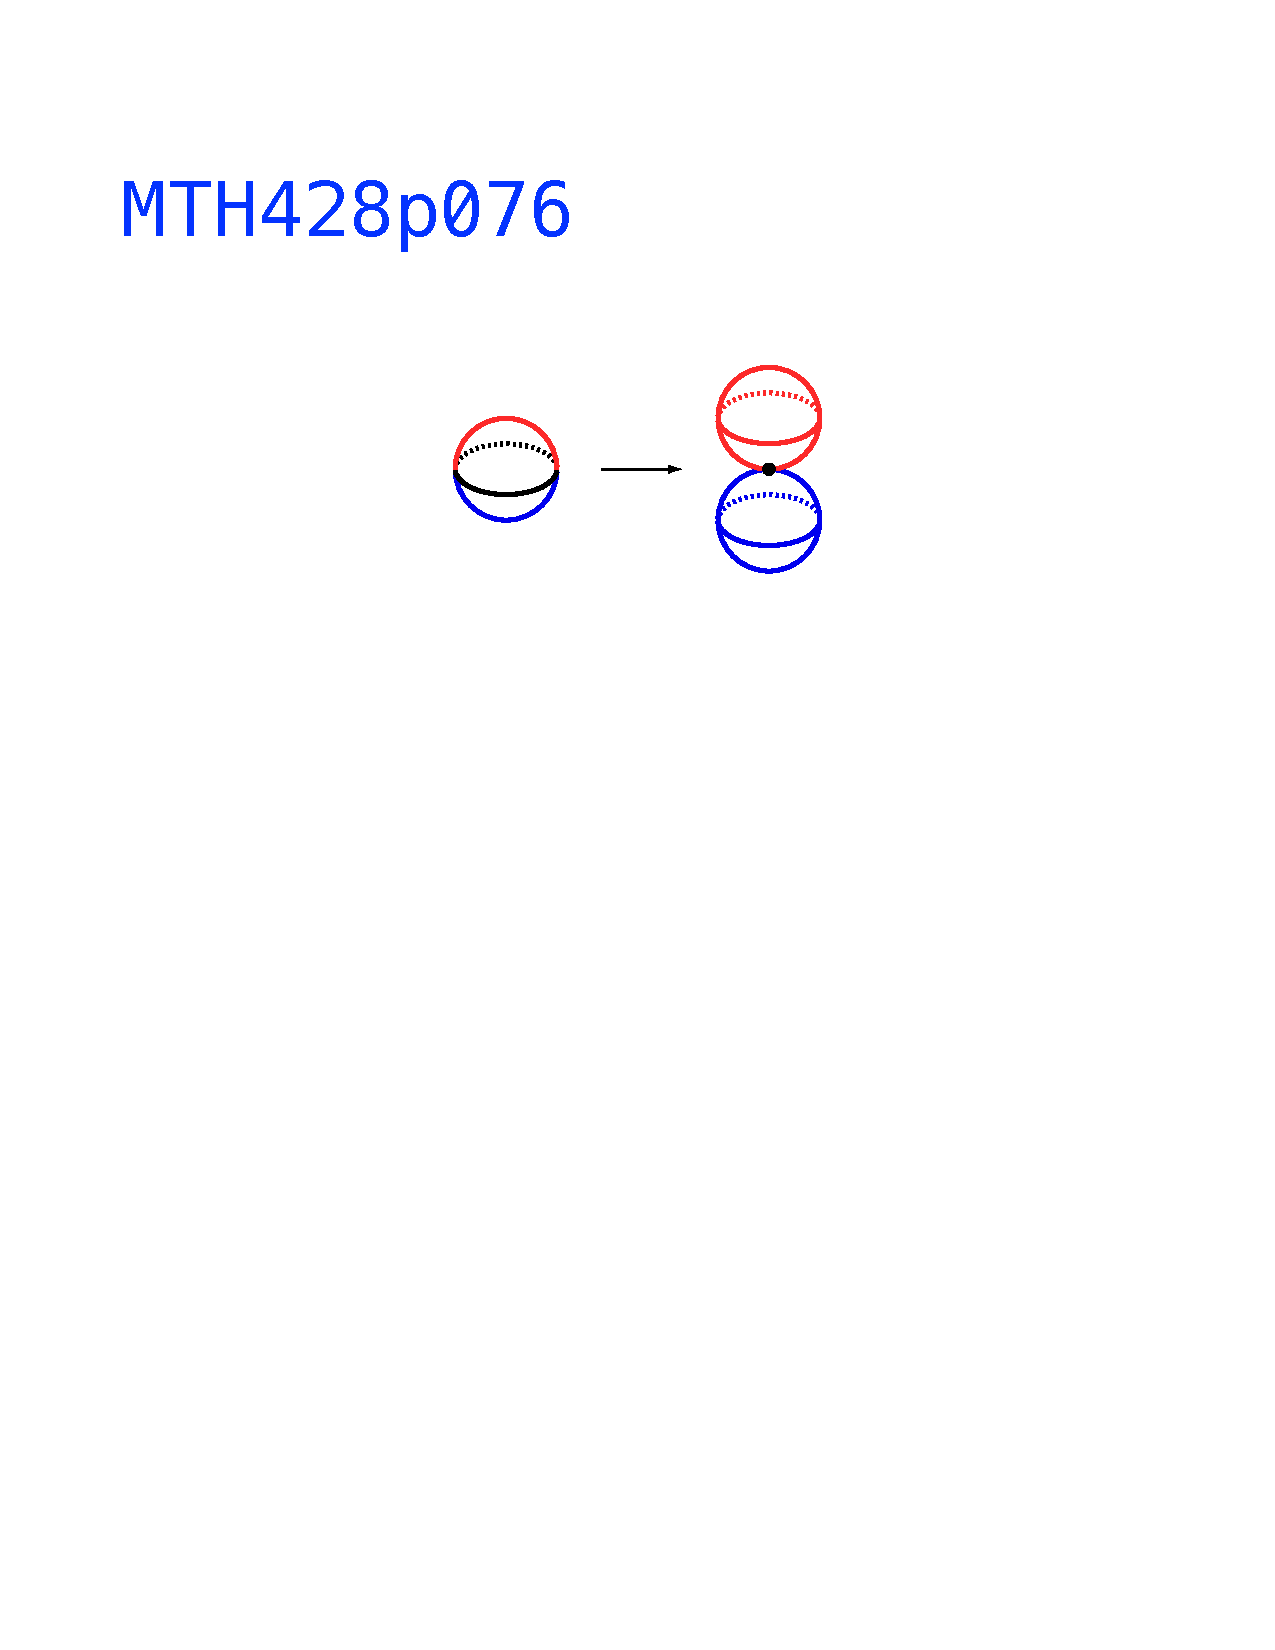
\includegraphics[width=\textwidth, trim=0mm 182mm 0mm 61mm, clip]{pictures/MTH428p076.pdf}}};

%%% COORDINATE GRID
%\draw[step=0.5, help lines] (0,0) to[grid with coordinates] (15,9);
%%% 
\node[anchor= base]  at (8.4 , 1.8){\small  $p$};

\end{tikzpicture}


Given two basepoint preserving maps $\omega, \tau\colon (S^{n}, s_{0}) \to (X, x_{0})$ we can define a map 
$\omega\vee \tau \colon S^{n}\vee S^{n} \to X$ that maps the first copy of $S^{n}$ using $\omega$ and the second
copy using $\tau$. We set: $[\omega]\cdot [\tau] = [(\omega\vee \tau) \circ p]$. 


One can check that $\pi_{n}(X, x_{0})$ taken with this multiplication is a group. The trivial element in this group 
is given by the homotopy class of the constant map $(S^{n}, s_{0}) \to (X, x_{0})$. For $[\omega]\in \pi_{n}(X, x_{0})$ 
we have $[\omega]^{-1} = [\omega\circ f]$ where $f\colon S^{n} \to S^{n}$ is the map given by 
$f(x_{1}, x_{2}, \dots, x_{n}, x_{n+1}) = (x_{1}, x_{2}, \dots, x_{n}, -x_{n+1})$. 

The assignments $(X, x_{0}) \mapsto \pi_{n}(X, x_{0})$ define a functor
$\pi_{n} \colon\Top_{\ast} \to \Gr$.

\begin{theorem}
\label{PIN SN THM}
\ 

\benu
\item[1)] For any $m, n\geq 1$ and $x_{0}\in D^{m}$ the group $\pi_{n}(D^{m}, x_{0})$ is trivial. 
\item[2)] For any $n\geq 1$ and $x_{0}\in S^{n}$ there is an isomorphism $\pi_{n}(S^{n})\cong \Z$.  
\eenu
\end{theorem}

The proof of part 1) is easy and similar to the proof that $\pi_{1}(D^{m})$ is trivial for all $m\geq 1$
(see Proposition \ref{PI1 DN TRIVIAL PROP}). The second part is harder and requires  more work 
that the proof that $\pi_{1}(S^{1}) \cong \Z$.  Since our main focus in these notes is the fundamental group 
we will skip this proof. 

Theorem \ref{PIN SN THM} combined with the argument outlined above implies that  statement 1) on page \pageref{GENERAL BROUWER PAGE} holds. Using this, by the same argument as in the proof of  
Theorem \ref{BROUWER FIXED POINT THM}  we obtain statement 2). Higher homotopy groups can be also 
used to prove statement 3) which in turn implies statement 4). 

%---BBLANK
\begin{note}
%---EBLANK #  Relation to $\pi_{0}(X)$. \end{note} \newpage
Recall that in Example \ref{PI ZERO FUNCTOR EXAMPLE} we defined a functor $\pi_{0}$ 
that assigns to a space $X$ the set $\pi_{0}(X)$ of path connected components of $X$. This functor is 
related to the functors $\pi_{n}$ constructed above as follows. Recall that the 0-dimesional sphere is a discrete 
space consisting of two points $S^{0} = \{-1, 1\}$. Choose $1\in S^{0}$ as the basepoint. If $(X, x_{0})$ is 
a pointed space then any basepoint preserving map $f\colon (S^{0}, 1) \to (X, x_{0})$ is  determined 
by the value of $f(-1)$, and this value can be an arbitrary point of $X$. 
This gives a bijection:
$$
\begin{pmatrix}
\text{basepoint preserving maps} \\[1mm]
\text{$f\colon (S^{0}, 1) \to (X, x_{0})$} \\
\end{pmatrix}
\cong 
\begin{pmatrix}
\text{points} \\[1mm]
\text{of $X$} \\
\end{pmatrix} 
$$
$$
\ \ \ \ \ \ \ \ \ \ \ \ \ \ \ \ \ f \ \ \ \ \ \ \ \ \ \ \ \ \ \ \ \ \ \mapsto \ \ f(-1)
$$
It is also easy to see that giving a homotopy between maps $f, g\colon  (S^{0}, 1) \to (X, x_{0})$
is the same as giving a path between the points $f(-1)$ and $g(-1)$. This means that  maps 
$f, g$ are homotopic if and only if the points $f(-1)$ and $g(-1)$ are in the same path connected component
of $X$. As a consequence we obtain a bijection: 
$$
\begin{pmatrix}
\text{homotopy classes of maps} \\[1mm]
\text{$f\colon (S^{0}, 1) \to (X, x_{0})$} \\
\end{pmatrix}
\cong 
\begin{pmatrix}
\text{path connected} \\[1mm]
\text{components of $X$} \\
\end{pmatrix} 
= \pi_{0}(X)
$$
The difference between the functors $\pi_{0}$ and $\pi_{n}$ for $n> 0$ is that $\pi_{0}(X)$ is in general just 
a set, not a group. However, for any pointed space $(X, x_{0})$ the set $\pi_{0}(X)$ has a natural choice 
of a basepoint given by the path connected component of $x_{0}$ (or equivalently, by the homotopy class of the 
constant map $(S^{0}, 1) \to (X, x_{0})$). This means that we can consider $\pi_{0}$ as a functor 
$$\pi_{0}\colon \Top_{\ast} \to \Set_{\ast}$$
where $\Set_{\ast}$ denotes the category of pointed sets i.e. sets equipped with a basepoint. 

\end{note}

%---BBLANK  # Higher homotopy groups via maps $I^{n} \to X$.
%---EBLANK  # \newpage
The above description of higher homotopy groups generalizes the construction of the 
fundamental group given in (\ref{PI1THROUGHS1 NOTE}), using maps $S^{1}\to X$. We can also describe 
groups $\pi_{n}(X, x_{0})$ in a way paralleling the construction of $\pi_{1}(X, x_{0})$ that used loops 
$[0, 1]\to X$. Namely, let $I^{n} = \prod_{i=1}^{n} [0, 1]$ be the $n$-dimensional cube, and  let 
$\partial I^{n} = I^{n} \ssmin \prod_{i=1}^{n} (0, 1)$. Given a pointed space $(X, x_{0})$ by 
$\omega\colon (I^{n}, \partial I^{n}) \to (X, x_{0})$ we will denote a map $\omega\colon I^{n} \to X$ such that 
$\omega(\partial I^{n}) =  x_{0}$. We will say that to maps  $\omega, \tau\colon (I^{n}, \partial I^{n}) \to (X, x_{0})$ 
are homotopic if there exists a map $h\colon I^{n}\times [0,1] \to X$ such that $h(s, 0) = \omega(s)$,   
$h(s, 1) = \tau(s)$ for any $s\in I^{n}$, and $h(\partial I^{n} \times [0, 1]) = x_{0}$. We define $\pi_{n}(X, x_{0})$
as the set of homotopy classes of maps $(I^{n}, \partial I^{n}) \to (X, x_{0})$. For 
$\omega, \tau \colon (I^{n}, \partial I^{n}) \to (X, x_{0})$ define $\omega\ast\tau \colon (I^{n}, \partial I^{n}) \to (X, x_{0})$
by

$$
(\omega\ast \tau)(s_{1}, s_{2}, \dots, s_{n}) = 
\begin{cases}
\omega(2s_{1}, s_{2}, \dots, s_{n}) & \text{ for } s_{1}\in [0, \frac{1}{2}] \\
\tau(2s_{1} -1, s_{2}, \dots, s_{n}) & \text{ for } s_{1}\in [\frac{1}{2}, 1] \\
\end{cases}
$$ 

\begin{equation*}
\begin{tikzpicture}
\draw[very thick] (0,0) rectangle  node[anchor=center] {$\omega$} (1,2);
\draw[very thick] (1,0) rectangle node[anchor=center] {$\tau$}(2,2);
\end{tikzpicture}
\end{equation*}

One can check that this induces a well-defined associative multiplication 
$$\pi_{n}(X, x_{0}) \times\pi_{n}(X, x_{0}) \to \pi_{n}(X, x_{0})$$
given by $[\omega]\cdot [\tau] = [\omega\ast \tau]$ which makes $\pi_{n}(X, x_{0})$ into a group. The trivial element 
of $\pi_{n}(X, x_{0})$ is the homotopy class of the constant map $c_{x_{0}}\colon I^{n} \to X$. Also, for 
$[\omega]\in \pi_{1}(X, x_{0})$ we have $[\omega]^{-1} = [\xov{\omega}]$ where 
$\xov{\omega}\colon  (I^{n}, \partial I^{n}) \to (X, x_{0})$ is given by 
$$\xov{\omega}(s_{1}, s_{2}, \dots, s_{n}) = (1-s_{1}, s_{2}, \dots, s_{n})$$


We will see later that the fundamental group of a space need not be commutative. By contrast we have:

%---BBLANK 
\begin{theorem}
For $n\geq 2$ then the group $\pi_{n}(X, x_{0})$ is abelian for any  pointed space $(X, x_{0})$.   
\end{theorem}
%---EBLANK  #\newpage


\begin{proof}
A homotopy $\omega\ast\tau \simeq \tau\ast\omega$ can be depicted as follows:

\begin{equation*}
\begin{tikzpicture}
\draw[very thick] (0,0) rectangle  node[anchor=center] {$\omega$} (1,2);
\draw[very thick] (1,0) rectangle node[anchor=center] {$\tau$}(2,2);
\node at (2.5,1) {$\simeq$};
\draw[very thick] (3,0) rectangle  node[anchor=center] {$\omega$} (4,1);
\draw[very thick] (4,1) rectangle node[anchor=center] {$\tau$}(5,2);
\draw[very thick, fill=mygray2] (3,1) rectangle node[anchor=center] {$x_{0}$}(4,2);
\draw[very thick,  fill=mygray2] (4,0) rectangle node[anchor=center] {$x_{0}$}(5,1);
\node at (5.5,1) {$\simeq$};
\draw[very thick] (6,0) rectangle  node[anchor=center] {$\omega$} (8,1);
\draw[very thick] (6,1) rectangle node[anchor=center] {$\tau$}(8,2);
\node at (8.5,1) {$\simeq$};
\draw[very thick,  fill=mygray2] (9,0) rectangle  node[anchor=center] {$x_{0}$} (10,1);
\draw[very thick,  fill=mygray2] (10,1) rectangle node[anchor=center] {$x_{0}$}(11,2);
\draw[very thick] (9,1) rectangle node[anchor=center] {$\tau$}(10,2);
\draw[very thick] (10,0) rectangle node[anchor=center] {$\omega$}(11,1);
\node at (11.5,1) {$\simeq$};
\draw[very thick] (12,0) rectangle  node[anchor=center] {$\tau$} (13,2);
\draw[very thick] (13,0) rectangle node[anchor=center] {$\omega$}(14,2);
\end{tikzpicture}
\end{equation*}
The shaded squares in the pictures are mapped to the basepoint $x_{0}\in X$.

\end{proof}


%%%%%%%%%%%%%%%%%%%%%%%%%%%%%%%
%  EXERCISES
%%%%%%%%%%%%%%%%%%%%%%%%%%%%%%%

\exercises

\begin{exercise}
\label{PI1SN TRIVIAL EXERCISE}
Show that the fundamental group of the sphere $S^{n}$ is trivial for $n>1$.  (Hint: show first that any loop $\omega\colon [0, 1] \to S^{n}$
is homotopic to a loop $\omega'\colon [0, 1]\to S^{n}$ which is not onto.)
\end{exercise}


\newpage
%%%%%%%%%%%%%%%%%%%%%%%%%%%%%%%
%%%%%%%%%%%%%%%%%%%%%%%%%%%%%%%
%%%
%%%  HOMOTOPY INVARIANCE 
%%%
%%%%%%%%%%%%%%%%%%%%%%%%%%%%%%%
%%%%%%%%%%%%%%%%%%%%%%%%%%%%%%%

%---BBLANK  
\chapter{Homotopy Invariance }
%---EBLANK 
\chaptermark{Homotopy Invariance}

\thispagestyle{firststyle}

So far we computed the fundamental group for very few  spaces. In order to extend these 
computations to other spaces we will use three basic tools: homotopy invariance of $\pi_{1}$, the product 
formula for $\pi_{1}$, and the van Kampen theorem. In this chapter we discuss the first of these topics and 
in the subsequent ones we deal with the other two. 

%---BBLANK  
\begin{definition}
\label{HOMOTOPY DEF}
Let $f, g\colon X \to Y$ be continuous functions. A \emph{homotopy} between $f$ and $g$ is a continuous 
function $h\colon X\times [0, 1]\to Y$ such that $h(x, 0) = f(x)$ and $h(x, 1) = g(x)$: 

\begin{equation*}
\begin{tikzpicture}[
    scale = 2.3,
    d0/.style = {line width = 1.6pt},
    d1/.style= {postaction={decorate}, line width = 1.6pt, decoration={markings, mark=at position 0.55 with {\arrow{stealth}}}},
    d2/.style = {postaction={decorate}, line width = 1.6pt, decoration={markings, mark=at position 0.54 with {\arrow[rotate=9]{stealth}}}},
]

\draw[d0, fill = mygray1] (0,0) rectangle node{\small $X\times [0, 1]$} (1,1);
\draw[d0, red]  (0,0) node[anchor = east] {\small $X\times \{0\}$}  --  (1, 0); 
\draw[d0, red]  (0,1) node[anchor = east] {\small $X\times \{1\}$}  --  (1, 1); 
\draw[d0, red]  (0,1) -- (1,1); 
\draw[thick, fill= mygray1, scale = 0.5, shift={(2, -0.95)}] 
plot [smooth cycle, tension = 0.9] coordinates{(2, 1.5) (3, 1.0) (4, 2.0)  (3, 3) (2, 2.5) } ;
\node at (2.4, 0.5) {\small $Y$};
\draw[thick, ->, >=latex] (1.2, 0.5) -- node[anchor=south] {\small $h$} (1.7, 0.5);
\draw[red,thick, ->, >=latex] (0.7, 1.1) arc (125:55:1.3) node[pos= 0.5, anchor=south] {\small $g$};
\draw[red,thick, ->, >=latex] (0.7, -0.1) arc (-125:-55:1.3) node[pos= 0.5, anchor=north] {\small $f$};
\end{tikzpicture}
\end{equation*}


If such homotopy exists then we say that the functions $f$ and $g$ are \emph{homotopic} 
and we write $f\simeq g$.  We will also write $h\colon f\simeq g$ to indicate that $h$ is a homotopy 
between $f$ and $g$.  
\end{definition}



%---EBLANK   # \newpage

\begin{note}
Given a homotopy $h\colon X \times [0, 1] \to Y$ it will be convenient denote by $h_{t}\colon X \to Y$
the function defined by $h_{t}(x) = h(x, t)$. If $h\colon f\simeq g$ then $h_{0} = f$ and $h_{1} = g$. 
\end{note}


\begin{example}
\label{HOMOTTORN EX}
Any two functions $f, g\colon X \to \R^{n}$ are homotopic. Indeed, define 
$h\colon X \times [0, 1] \to \R$ by $h(x, t) = (1-t)f(x) + tg(x)$. Then $h_{0} = f$ and $h_{1} = g$. 
\end{example}

A useful generalization of Definition \ref{HOMOTOPY DEF} is the notion of a relative homotopy:

%---BBLANK  
\begin{definition}
Let $X$ be a space and let $A\subseteq X$. If $f, g\colon X \to Y$ are functions such that $f|_{A} = g|_{A}$
then we say that $f$ and $g$ are \emph{homotopic relative to $A$} if there exists a homotopy 
$h\colon X \times [0, 1] \to Y$ such that $h_{0} = f$, $h_{1} = g$ and $h_{t}|_{A} = f|_{A} = g|_{A}$ for all 
$t\in [0, 1]$. In  such case we write $f\simeq g \ (\rel A)$. 
\end{definition}
%---EBLANK  # \vskip 50mm

\begin{example}
Let $\omega, \tau\colon [0, 1] \to X$ be paths in $X$. Recall that path homotopy is defined only 
if $\omega|_{\{0, 1\}} = \tau|_{\{0, 1\}}$  and it is given by a map $h\colon [0, 1]\times [0, 1] \to X$
such that $h_{0} = \omega$, $h_{1} = \tau$ and $h_{t}|_{\{0, 1\}} = \omega|_{\{0, 1\}} = \tau|_{\{0, 1\}}$
for each $t\in [0, 1]$.  Thus, in  the paths $\omega$ and $\tau$ are path homotopic if and only if 
$\omega \simeq \tau \ (\rel \{0, 1\})$. 
\end{example}

%---BBLANK  
\begin{definition}
\label{HOMOTEQ DEF}
A map $f\colon X \to Y$ is a \emph{homotopy equivalence} if there exists a map $g\colon Y \to X$ 
such that $gf \simeq \id_{X}$ and $fg\simeq \id_{Y}$. If such maps exist  we say that the spaces
$X$ and $Y$ are \emph{homotopy equivalent} and we write $X \simeq Y$. 
\end{definition}
%---EBLANK  

\begin{note}
If $f$ and $g$ are maps as in Definition \ref{HOMOTEQ DEF} then we say that $g$ is 
a \emph{homotopy inverse} of $f$.  
\end{note}

\begin{example}
\label{RN CONTRACTIBLE EX}
We will show $\R^{n}$ is homotopy equivalent to the space $\{\ast\}$ consisting of a single point. 
Let $f\colon \R^{n} \to \{\ast\}$ be the constant function and let $g\colon \{\ast\} \to \R^{n}$ be given by 
$f(\ast) = x_{0}$ for some $x_{0}\in \R^{n}$. We have $fg = \id_{\{\ast\}}$ so $fg\simeq \id_{\{\ast\}}$. 
On the other hand by Example \ref{HOMOTTORN EX} any two functions into $\R^{n}$ are homotopic, 
so in particular $gf \simeq \id_{\R^{n}}$
\end{example}

\begin{note}
Example \ref{RN CONTRACTIBLE EX} shows that a homotopy inverse of a homotopy equivalence 
$f\colon X \to Y$ in general is not unique: any function $g\colon \{\ast\} \to \R^{n}$ is a homotopy 
inverse of the constant function $f\colon \R^{n} \to \{\ast\}$. 
\end{note}

%---BBLANK  # \vskip 60mm
\begin{definition}
If $X$ is a space such that $X \simeq \{\ast\}$ then we say that $X$ is a \emph{contractible space}. 
\end{definition}
%---EBLANK  # 

%---BBLANK  # \vskip 10mm
\begin{proposition}
Let $X$ be a topological space. The following conditions are equivalent:
\benu
\item[1)] $X$ is contractible; 
\item[2)] the identify map $\id_{X}$ is homotopic to a constant map; 
\item[3)] for each  space $Y$ and any maps $f, g\colon Y \to X$ we have $f\simeq g$. 
\eenu
\end{proposition}

\begin{proof}
Exercise. 
\end{proof}
%---EBLANK  # \newpage

Many examples of homotopy equivalences can be  obtained  using deformation retractions:

%---BBLANK  
\begin{definition}
A subspace $A \subseteq X$ is a \emph{deformation retract} of a space $X$ if there exists a homotopy 
$h\colon X \times [0, 1] \to X$ such that 
\benu
\item[1)] $h_{0} = \id_{X}$
\item[2)] $h_{t}|_{A} = \id_{A}$ for all  $t\in [0, 1]$ 
\item[3)] $h_{1}(x)\in A$ for all $x\in X$
\eenu
In such case we say that $h$ is a \emph{deformation retraction}
of $X$ onto $A$. 

\end{definition}  
%---EBLANK 


%---BBLANK  # \vskip 50mm
\begin{proposition}
If $A\subseteq X$ is a deformation retract of $X$ then $A\simeq X$. 
\end{proposition}
%---EBLANK # \newpage

\begin{proof}
Let $h\colon X \times [0, 1]\to X$ be a deformation retraction, let $r\colon X \to A$ be given by 
$r(x) = h_{1}(x)$ and let $j\colon A \to X$ be the inclusion map. We have $rj = \id_{A}$. Also, 
$h$ is a homotopy between $\id_{X}$ and $jr$. 
\end{proof}


\begin{example}
\label{DEFRETR EX}
For any $n > 0$ the sphere $S^{n-1}$ is a deformation retract of $\R^{n}\ssmin \{0\}$. 
Indeed, a deformation retraction $h\colon \R^{n}\ssmin \{0\} \to S^{n-1}$ is given by 
$$h(x, t) = \frac{x}{(1-t) + t\norm{x}}$$
As a consequence $\R^{n}\ssmin \{0\} \simeq S^{n-1}$.
\end{example}


Interesting examples of homotopy equivalences can be also obtained using the constructions 
of a mapping cylinder and a mapping cone:

%---BBLANK  
\begin{definition} 
%---EBLANK #  Mapping cylinder and mapping cone. \end{definition}
\label{MAP CYL CONE DEF}
Let $f\colon X \to Y$ be a continuous function. 
The \emph{mapping cylinder} of $f$ is 
the space 
$$M_{f} = (X \times [0, 1] \sqcup Y) /{\sim}$$ 
where $\sim$ is the equivalence relation given by $(x, 1) \sim f(x)$ for all $x\in X$. 

\begin{equation*}
\begin{tikzpicture}[
    scale = 1.7,
    d0/.style = {line width = 1.6}
]


\draw[d0, fill = mygray1] (0,0.6) rectangle node {\small $X \times [0, 1]$} (1.0, 1.7) ;
\draw[d0, red] (0,0.6) -- (1.0, 0.6) node[pos= 1.95, anchor = east] {\small $X \times \{1\}$};
\draw[d0] (-0.4, 0) -- node[pos = 0.05, anchor=south] {\small $Y$} (1.4, 0);
\draw[d0, red, line cap=rect] (0.15, 0) -- (0.85, 0) node[anchor = north, pos=0.5] {\small $f(X)$};
\draw[thick, red, ->, >=latex] (0.5, 0.5) -- node[anchor = west] {\small $f$} (0.5, 0.1);

\draw[thick, ->, >=latex] (1.95, 0.3) -- (2.6, 0.3);

\begin{scope}[shift ={(3.5, 0)}]
\draw[d0, fill = mygray1] (0.15,0.0) -- (0.0, 1.1) -- (1.0, 1.1) -- (0.85, 0) -- cycle;
\draw[d0] (-0.4, 0) --(1.4, 0);
\draw[d0, red, line cap=rect] (0.15, 0) -- (0.85, 0)  node[anchor = north, pos=0.5, black] {\small $M_{f}$};
\end{scope}


\end{tikzpicture}
\end{equation*}





The \emph{mapping cone} of $f$ is the space obtained from $M_{f}$ by collapsing the subspace 
$X\times\{0\} \subseteq M_{f}$ to a point:
$$C_{f} = M_{f}/(X\times \{0\})$$



\begin{equation*}
\begin{tikzpicture}[
    scale = 1.7,
    d0/.style = {line width = 1.6}
]


\draw[d0, fill = mygray1] (0.15,0.0) -- (0.0, 1.1) -- (1.0, 1.1) -- (0.85, 0) -- cycle;
\draw[d0, red] (0, 1.1) --(1.0, 1.1) node[pos= 1.95, anchor = east] {\small $X \times \{0\}$};
\draw[d0]  (-0.4, 0) --(1.4, 0)  node[anchor = north, pos=0.5] {\small $M_{f}$};

\draw[thick, ->, >=latex] (1.95, 0.3) -- (2.6, 0.3);

\begin{scope}[shift ={(3.5, 0)}]
\draw[d0, fill = mygray1] (0.15, 0.0) -- (0.5, 1.1) -- (0.85, 0) -- cycle;
\draw[d0] (-0.4, 0) --(1.4, 0) node[anchor = north, pos=0.5] {\small $C_{f}$};
\filldraw[d0, red] (0.5, 1.1)  circle (0.035);
\end{scope}


\end{tikzpicture}
\end{equation*}



\end{definition}

%---BBLANK  # \vskip 90mm
\begin{proposition}
For any map $f\colon X \to Y$ we have $M_{f}\simeq Y$. 
\end{proposition}


\begin{proof}
Exercise. 
\end{proof}
%---EBLANK  


%---BBLANK  # \vskip 30mm
\begin{proposition}
\label{CONESLIDE PROP}
Let $f, g\colon X \to Y$ be continuous functions. If $f\simeq g$ then $C_{f}\simeq C_{g}$.
\end{proposition}

\begin{proof}
Exercise. 
\end{proof}
%---EBLANK  # \newpage

%---BBLANK  
\begin{example}
%---EBLANK  # \end{example} \newpage
\label{MAPCONECYL EX}
Consider maps $f, g\colon \{-1, 1\} \to S^{1}$ where $f$ is a constant map and $g$ is non-constant
(e.g. $g$ maps $1$ and $-1$ to antipodal points of $S^{1}$). 
Mapping cylinders of the these functions can be depicted as follows:


\begin{equation*}
\begin{tikzpicture}[scale = 0.66]
\begin{scope}
\draw[line width = 1.6pt] (0,0) circle (1);
\draw[line width = 1.6pt] (-1, 2.5) -- (0, 1) -- (1, 2.5);
\draw[red, fill = red] (0,1) circle (0.12);
\draw[red, fill = red] (-1,2.5) circle (0.12);
\draw[red, fill = red] (1,2.5) circle (0.12);
\node[anchor= north] at (0, -1.2) {\small $M_{f}$};
\end{scope}
\begin{scope}[xshift = 200pt]
\draw[line width = 1.6pt] (0,0) circle (1);
\draw[line width = 1.6pt] (-1, 2.5) -- (-1, 0)  (1, 2.5) -- (1, 0);
\draw[red, fill = red] (-1,0) circle (0.12);
\draw[red, fill = red] (1,0) circle (0.12);
\draw[red, fill = red] (-1,2.5) circle (0.12);
\draw[red, fill = red] (1,2.5) circle (0.12);
\node[anchor= north] at (0, -1.2) {\small $M_{g}$};
\end{scope}
\end{tikzpicture}
\end{equation*}


The mapping cones, in turn, look as follows:

\begin{equation*}
\begin{tikzpicture}[scale = 0.66]
\begin{scope}
\draw[line width = 1.6pt] (0,0) circle (1);
\draw[line width = 1.6pt] (0, 2.5) ..controls (.6, 2.1) and (.6, 1.4).. (0, 1);
\draw[line width = 1.6pt] (0, 2.5) ..controls (-.6, 2.1) and (-.6, 1.4).. (0, 1);
\draw[red, fill = red] (0,1) circle (0.12);
\draw[red, fill = red] (0,2.5) circle (0.12);
\node[anchor= north] at (0, -1.2) {\small $C_{f}$};
\end{scope}
\begin{scope}[xshift = 200pt]
\draw[line width = 1.6pt] (0,0) circle (1);
\draw[line width = 1.6pt] (-1, 0) ..controls (-1, 1)  and (-0.4, 2.3).. (0, 2.5);
\draw[line width = 1.6pt] (1, 0) ..controls (1, 1)  and (0.4, 2.3).. (0, 2.5);
\draw[red, fill = red] (-1,0) circle (0.12);
\draw[red, fill = red] (1,0) circle (0.12);
\draw[red, fill = red] (0,2.5) circle (0.12);
\node[anchor= north] at (0, -1.2) {\small $C_{g}$};
\end{scope}
\end{tikzpicture}
\end{equation*}


Notice that  $f\simeq g$, and so $C_{f} \simeq C_{g}$. Notice also that the space $C_{f}$ is homeomorphic 
to $S^{1}\vee S^{1}$ while $C_{g}$ is homeomorphic to the space obtained as a union of $S^{1}$ 
and one of its diagonals. In effect we obtain a homotopy equivalence:


\begin{equation*}
\begin{tikzpicture}[scale = 0.6]
\draw[line width = 1.6pt] (6,0) circle (1);
\draw[line width = 1.6pt] (5, 0) -- (7, 0);
\draw[line width = 1.6pt] (0,1) circle (1);
\draw[line width = 1.6pt] (0,-1) circle (1);
\node[anchor = base] at (3,0) { $\simeq$};
\end{tikzpicture}
\end{equation*}


 
\end{example}

Our next goal is to examine how the fundamental group behaves with respect to homotopic 
maps and homotopy equivalent spaces. First, recall that a map of pointed spaces 
$f\colon (X, x_{0}) \to (Y, y_{0})$ induces a homomorphism of fundamental groups 
$f_{\ast}\colon \pi_{1}(X, x_{0}) \to \pi_{1}(Y, y_{0})$ which is given by $f_{\ast}([\omega]) = [f\circ \omega]$. 
We have:

%---BBLANK  
\begin{proposition}
\label{PI1 HOMOTINVRELBASEPOINT PROP}
If $f, g\colon (X, x_{0}) \to (Y, y_{0})$ are maps of pointed spaces such that $f\simeq g \ (\rel \{x_{0}\})$
then $f_{\ast} = g_{\ast}$. 
\end{proposition}
%---EBLANK  # \vskip 70mm

\begin{proof}
For $[\omega]\in \pi_{1}(X, x_{0})$ we want to show that $f_{\ast}([\omega]) = g_{\ast}([\omega])$, or 
equivalently that 
$$f\circ \omega \simeq g\circ \omega \ \ (\rel \{0, 1\})$$
Let $h\colon X\times [0, 1] \to Y$ be a homotopy between $f$ and $g$ $(\rel \{x_{0}\})$. Then 
the map 
$$h\circ (\omega\times \id_{[0, 1]}) \colon [0, 1]\times [0, 1] \to Y$$
gives a path homotopy between $f\circ \omega$ and $g\circ \omega$. 
\end{proof}

Proposition \ref{PI1 HOMOTINVRELBASEPOINT PROP} can be generalized to the setting 
where we do not assume that homotopy preserves basepoints. Recall 
(\ref{FUND GP PATH ISO PROP}) that if $Y$ is a space, $y_{0}, y_{1}\in Y$ 
then a path $\tau$ in $Y$ with $\tau(0) = y_{0}$ and $\tau(1) = y_{1}$ induces an 
isomorphism $s_{\tau}\colon \pi_{1}(Y, y_{0}) \to \pi_{1}(Y, y_{1})$ given by  
$s_{\tau}([\omega]) = [\xov{\tau}\ast\omega\ast \tau]$.


%---BBLANK  
\begin{proposition}
\label{PI1 HOMOTINV PROP}
Let $f, g \colon X \to Y$ be homotopic maps and let $h\colon f\simeq g$. For $x_{0}\in X$ let $\tau$ 
be the path in $Y$ given by $\tau(t) = h(x_{0}, t)$. The following diagram commutes:
\begin{equation*}
\begin{tikzpicture}
\matrix (m) 
[matrix of math nodes, row sep=1em, column sep=3em, text height=1.5ex, text depth=0.25ex]
{
 & \pi_{1}(Y, f(x_{0})) \\
 \pi_{1}(X, x_{0}) &  \\
 & \pi_{1}(Y, g(x_{0})) \\
};
\path[->, thick, font=\scriptsize]
(m-2-1) 
edge node[anchor = south east] {$f_{\ast}$} (m-1-2)
edge node[anchor = north east] {$g_{\ast}$} (m-3-2)
(m-1-2)
edge node[anchor=  west] {$s_{\tau}$} node[anchor= east] {$\cong$} (m-3-2)

; 
\end{tikzpicture}
\end{equation*}
\end{proposition}

\begin{proof}
Exercise. 
\end{proof}
%---EBLANK  

%---BBLANK  # \vskip 30mm
\begin{corollary}
\label{PI1 HOMOTINV COR}
If $f, g\colon X \to Y$ are maps such that $f\simeq g$ then the homomorphism 
$f_{\ast}\colon \pi_{1}(X, x_{0}) \to \pi_{1}(Y, f(x_{0}))$ is an isomorphism (or is trivial or is 1-1 or onto)
if and only if the homomorphism $g_{\ast}\colon \pi_{1}(X, x_{0}) \to \pi_{1}(Y, g(x_{0}))$ has the same 
property. 
\end{corollary}
%---EBLANK  # \newpage


%---BBLANK  
\begin{proposition}
\label{HOMOTEQ PI1 PROP}
If $f\colon X \to Y$ is a homotopy equivalence then for any $x_{0}\in X$ the homomorphism 
$f_{\ast}\colon \pi_{1}(X, x_{0}) \to \pi_{1}(Y, f(x_{0}))$ is an isomorphism. 
\end{proposition}
%---EBLANK  

\begin{proof}
Let $g\colon Y \to X$ be a homotopy inverse of $f$. Consider the sequence of homomorphisms 
$$\pi_{1}(X, x_{0}) \overset{f_{\ast}}{\lra} \pi_{1}(Y, f(x_{0})) 
\overset{g_{\ast}}{\lra} \pi_{1}(X, gf(x_{0}))
\overset{f_{\ast}}{\lra} \pi_{1}(Y, fgf(x_{0})) $$
Composition of the first two homomorphisms satisfies $g_{\ast}f_{\ast} = (gf)_{\ast}$. Since 
$gf\simeq \id_{X}$ and $\id_{X\ast}$ is an isomorphism by Proposition \ref{PI1 HOMOTINV COR}
we obtain that $g_{\ast}f_{\ast}$ is an isomorphism. This implies in particular that $g_{\ast}$ is onto. 
Similarly, composing the last two homomorphisms we obtain $f_{\ast}g_{\ast} = (fg)_{\ast}$
and since $fg\simeq \id_{Y}$ we get that $f_{\ast}g_{\ast}$ is an isomorphism. This means
that $g_{\ast}$ is 1-1. As a consequence $g_{\ast}$ is an isomorphism. It follows that the first 
homomorphism $f_{\ast}$ is a composition of two isomorphisms: $f_{\ast} = g_{\ast}^{-1}(g_{\ast}f_{\ast})$, 
and so $f_{\ast}$ is an isomorphism. 


\end{proof}

%---BBLANK  # \vskip 60mm
\begin{corollary}
\label{PATHCON HOMOTEQ PI1 ISO COR}
If $X$, $Y$ are path connected spaces and $X \simeq Y$ then $\pi_{1}(X, x_{0}) \cong \pi_{1}(Y, y_{0})$
for any $x_{0}\in X$, $y_{0}\in Y$. 
\end{corollary}
%---EBLANK  # \newpage

\begin{proof}
Let $f\colon X\to Y$ be a homotopy equivalence. By Proposition \ref{HOMOTEQ PI1 PROP}
we get an isomorphism $f_{\ast}\colon \pi_{1}(X, x_{0}) \overset{\cong}{\lra} \pi_{1}(Y, f(x_{0}))$.  
Since $Y$ is path connected by Corrolary \ref{FUND GP PATH CONN ISO COR} we also have 
$\pi_{1}(Y, f(x_{0})) \cong \pi_{1}(Y, y_{0})$. 
\end{proof}

\begin{note}
In the proof above we  used only that $Y$ is path connected, so the assumption in 
Corollary \ref{PATHCON HOMOTEQ PI1 ISO COR} that both $X$ and $Y$ are path connected 
may seem too strong. However, if $Y$ is path connected and $X\simeq Y$ then $X$ must be 
path connected as well (exercise). 
\end{note}

\begin{example} As we have seen before (\ref{DEFRETR EX}) the space  $\R^{n}\ssmin \{0\}$
is homotopy equivalent to the sphere $S^{n-1}$. This gives
$\pi_{1}(\R^{n}\ssmin \{0\}) \cong \pi_{1}(S^{n-1})$. In particular 
$\pi_{1}(\R^{2}\ssmin\{0\}) \cong \pi_{1}(S^{1})\cong \Z$. 
\end{example}

\begin{example} 
Let $\Theta$ be the space obtained as a union of $S^{1}$ and one of its diagonals. 
By Example \ref{MAPCONECYL EX} this space is homotopy equivalent to $S^{1}\vee S^{1}$, 
so $\pi_{1}(\Theta) \cong \pi_{1}(S^{1}\vee S^{1})$. 
\end{example}


%%%%%%%%%%%%%%%%%%%%%%%%%%%%%%%
%  EXERCISES
%%%%%%%%%%%%%%%%%%%%%%%%%%%%%%%

\exercises

\begin{exercise}
Recall that if $X$  is a space then $\pi_{0}(X)$ denotes the set of path connected components 
of $X$. If $x\in X$ then by $[x]\in \pi_{0}(X)$ we will denote the path connected component 
of the point $x$. Recall that a continuous function $f\colon X \to Y$ induces a map of sets 
$f_{\ast}\colon \pi_{0}(X) \to \pi_{0}(Y)$ given by $\pi_{0}([x]) = [f(x)]$. Show that if 
$f$ is a homotopy equivalence then $f_{\ast}$ is a bijection. 
\end{exercise}





\begin{exercise}
Let $f, g\colon X \to Y $ be two homeomorphisms and let $f^{-1}, g^{-1}\colon Y\to X$
be their respective inverses. Show that if $f\simeq g$ then $f^{-1}\simeq g^{-1}$. 
\end{exercise}

\begin{exercise}
a) For $i=1, 2$ let $X_{i}$ be a topological space and let $Y_{i}\subseteq X_{i}$. Assume that 
we have a commutative  diagram:
\begin{equation*}
\begin{tikzpicture}
\matrix (m) 
[matrix of math nodes, row sep= 2.5em, column sep=2.5em, text height=1.5ex, text depth=0.25ex]
{
Y_{1} &  X_{1} &  Y_{1} \\
Y_{2} & X_{2} & Y_{2} \\
};
\path[->, thick, font=\scriptsize]
(m-1-1) 
edge node[auto] {$j_{1}$} (m-1-2)
edge node[anchor=east] {$f'$} (m-2-1)
(m-1-2) 
edge node[auto] {$r_{1}$} (m-1-3)
edge node[auto] {$f$} (m-2-2)
(m-1-3) 
edge node[auto] {$f'$} (m-2-3)
(m-2-1) 
edge node[anchor=north] {$j_{2}$} (m-2-2)
(m-2-2) 
edge node[anchor=north] {$r_{2}$}(m-2-3)
;
\end{tikzpicture}
\end{equation*}
where  $j_{i}\colon Y_{i}\to X_{i}$ is the inclusion map, and $r_{i}\colon X_{i}\to Y_{i}$
is a retraction.  Show that if $f$ is a homotopy equivalence then $f'$ is a homotopy equivalence as well. 


b) Let $X$ be a contractible space and let $A\subseteq X$ be a retract of $X$. Show that $A$
is contractible. 
\end{exercise}


\begin{exercise}
For spaces $X$ and $Y$ let $[X, Y]$ denote the set of homotopy classes of maps $X \to Y$. That is, each map $f\colon X \to Y$
defines an element $[f]\in [X, Y]$ and $[f] = [f']$ if $f\simeq f'$. Notice that any map $g\colon X \to X'$ defines a function 
$g^{\ast}\colon [X', Y] \to [X, Y]$ given by $g^{\ast}([f]) = [fg]$.

Given a map $g\colon X \to X'$ show that the following conditions are equivalent:

\benu
\item[1)] The map $g$ is a homotopy equivalence. 

\item[2)] For each space $Z$ the function $g^{\ast}\colon [X', Z] \to [X, Z]$ is a bijection. 
\eenu

\end{exercise}






\begin{exercise}
The antipodal map  $f\colon S^{n} \to S^{n}$ is the map given by $f(x) = -x$. 
Show that if $g\colon S^{n}\to S^{n}$ is any map such that $g(x)\neq x$
for all $x\in S^{n}$ then $g\simeq f$. 
\end{exercise}




\begin{exercise}
Let $X$ be a topological  space. Assume that $f, g \colon X \to S^{n}$ are maps such that for some 
non-empty open set $U\subseteq S^{n}$ we have $f^{-1}(U) = g^{-1}(U) = V \subseteq X$  and 
$f|_{V} = g|_{V}$. Show that $f\simeq g$.  
\end{exercise}




\begin{exercise}
Prove Proposition \ref{CONESLIDE PROP}. 
\end{exercise}

 


\begin{exercise}
Prove Proposition \ref{PI1 HOMOTINV PROP}. 
\end{exercise}




\begin{exercise}
Let  $M$ be the M\"obius band and let $\partial M$ denote the boundary of $M$. 
Show that $\partial M$ is not a retract of $M$. 
\end{exercise}




\begin{exercise}
Recall (\ref{MAP CYL CONE DEF}) that the cone of a map $f\colon X \to Y$  is the space  
$$C_{f} =  (X\times [0, 1] \sqcup Y)/{\sim}$$
where $(x, 1) \sim f(x)$ for all $x\in X$ and $(x,0)\sim (x', 0)$ for all $x, x'\in X$. We 
can consider $Y$ as a subspace of $C_{f}$. Show that  $Y$ is contractible if any only 
if for every map $f\colon X \to Y$ the space $Y$ is a retract of $C_{f}$. 
\end{exercise}




\begin{exercise}
\label{S1 TO D2 EXT EXERCISE}
a) Let $f\colon S^{1} \to X$ be a continuous function. Show that $f$ is homotopic to a constant map 
if and only if there exists $\bar{f}\colon D^{2} \to X$ such that $\bar{f}|_{S^{1}} = f$. 

b) Show that if $f\colon S^{1} \to S^{1}$ is homotopic to a constant map then there exists $x_{0}\in S^{1}$
such that $f(x_{0}) = x_{0}$. 
\end{exercise}







\begin{exercise}
Let $F\colon D^{2} \to D^{2}$ be a function such that $F(S^{1}) \subseteq S^{1}$, and let  $f\colon S^{1}\to S^{1}$ 
be given by $f(x) = F(x)$  for all $x\in S^{1}$. Show that if $f$ is not homotopic to a constant map, then for each function $G\colon D^{2} \to D^{2}$ there is a point $x_{0}\in D^{2}$ such that $F(x_{0}) = G(x_{0})$.
\end{exercise}






\begin{exercise}
Recall that for $n\geq 1$ multiplication in the group $\pi_{n}(X, x_{0})$ can be defined using the pinch map 
$p\colon S^{n} \to S^{n}\vee S^{n}$: if $[\omega], [\tau]\in \pi_{n}(X, x_{0})$ then 
$[\omega]\cdot [\sigma] = [(\omega\vee \sigma)\circ p]$.
The goal of this exercise is to generalize this observation. 

For pointed spaces $(X,  x_{0})$ and $(Y, y_{0})$ let $[ X, Y]_{\ast}$ denote the set of pointed homotopy classes 
of maps $X\to Y$. That is, each pointed map $f\colon (X, x_{0}) \to (Y, y_{0})$ defines an element 
$[f]\in [ X, Y]_{\ast}$ and  $[f] = [g]$ if $f\simeq g$ relative the basepoint. Let $(X, x_{0})$ be a space such that 
\benu
\item[(i)] for each space $(Y, y_{0})$ the set $[ X, Y]_{\ast}$ has the structure of a group;
\item[(ii)] for each pointed map $f\colon (Y, y_{0}) \to  (Y', y'_{0})$ the induced function 
$f_{\ast}\colon [ X, Y]_{\ast}\to [ X, Y']_{\ast}$ is a group homomorphism. 
\eenu

a) Show that for any space space $(Y, y_{0})$ there exists a bijection of sets 
$\varphi_{Y}\colon [X\vee X, Y]_{\ast} \to [X, Y]_{\ast}\times [X, Y]_{\ast}$
such that for any pointed map $f\colon (Y, y_{0}) \to (Y', y_{0}')$ the following diagram commutes:
\begin{equation*}
\begin{tikzpicture}
\matrix (m) 
[ampersand replacement=\&, matrix of math nodes, row sep=3em, column sep=3em, text height=1.5ex, text depth=0.25ex]
{
\left[ X\vee X, Y\right]_{\ast} \& \left[X, Y\right]_{\ast} \times  \left[X, Y\right]_{\ast}\\
\left[ X\vee X, Y'\right]_{\ast} \& \left[X, Y'\right]_{\ast} \times  \left[X, Y'\right]_{\ast}\\
};
\path[->, thick, font=\scriptsize]
(m-1-1) 
edge node[auto] {$\varphi_{Y}$} node[anchor=  north] {$\cong$} (m-1-2)
edge node[anchor = east] {$f_{\ast}$} (m-2-1)
(m-1-2)
edge node[anchor=  west] {$f_{\ast}\times f_{\ast}$} (m-2-2)
(m-2-1)
edge node[anchor=  north] {$\varphi_{Y'}$} node[anchor=  south] {$\cong$} (m-2-2)
; 
\end{tikzpicture}
\end{equation*}



b) Show that there exists a map $p\colon X \to X\vee X$ such that for each space $(Y, y_{0})$ the multiplication 
in the group $[X, Y]_{\ast}$ is given by $[f]\cdot [g] = [(f\vee g)\circ p]$.


Hint: For a space $(Y, y_{0})$ let $\mu_{Y}$ denote the multiplication in the group $[X, Y]_{\ast}$:
$$\mu_{Y} \colon [X, Y]_{\ast} \times [X, Y]_{\ast} \to [X, Y]_{\ast}$$
Notice that the condition (ii) above is equivalent to saying that for any  map $f\colon (Y, y_{0}) \to  (Y', y'_{0})$
the following diagram commutes:
\begin{equation*}
\begin{tikzpicture}
\matrix (m) 
[matrix of math nodes, row sep=3em, column sep=3em, text height=1.5ex, text depth=0.25ex]
{
\left[X, Y\right]_{\ast} \times \left[X, Y\right]_{\ast} & \left[X, Y\right]_{\ast} \\
\left[X, Y'\right]_{\ast} \times \left[X, Y'\right]_{\ast} & \left[X, Y'\right]_{\ast} \\
};
\path[->, thick, font=\scriptsize]
(m-1-1) 
edge node[auto] {$\mu_{Y}$} (m-1-2)
edge node[anchor = east] {$f_{\ast}\times f_{\ast}$} (m-2-1)
(m-1-2)
edge node[anchor=  west] {$f_{\ast}$} (m-2-2)
(m-2-1)
edge node[anchor=  north] {$\mu_{Y'}$} (m-2-2)
; 
\end{tikzpicture}
\end{equation*}
\end{exercise}










\newpage
%%%%%%%%%%%%%%%%%%%%%%%%%%%%%%%
%%%%%%%%%%%%%%%%%%%%%%%%%%%%%%%
%%%
%%%  THE PRODUCT FORMULA
%%%
%%%%%%%%%%%%%%%%%%%%%%%%%%%%%%%
%%%%%%%%%%%%%%%%%%%%%%%%%%%%%%%

%---BBLANK
\chapter[The Product Formula]{The Product \\ Formula}
%---EBLANK
\chaptermark{The Product Formula}
\label{PRODUCT FORMULA CHAPTER}


\thispagestyle{firststyle}

Recall that if $G, H$ are groups then their direct product is the group $G\times H$
whose elements are pairs $(g, h)$ where $g\in G, h\in H$ and multiplication is given by 
$(g, h)\cdot (g', h') = (gg', hh')$. We have:

%---BBLANK
\begin{theorem}
\label{PI1PROD THM}
If $(X_{1}, x_{1})$, $(X_{2}, x_{2})$ are pointed spaces then 
$$\pi_{1}(X_{1}\times X_{2}, (x_{1}, x_{2})) \cong \pi_{1}(X_{1}, x_{1})\times \pi_{1}(X_{2}, x_{2})$$
\end{theorem}
%---EBLANK

\begin{proof}
For $i=1, 2$ let  $p_{i}\colon X_{1}\times X_{2} \to X_{i}$  be the projection map
$p_{i}(x_{1}, x_{2}) = x_{i}$. These maps induce homomorphisms 
$p_{i\ast}\colon \pi_{1}(X_{1}\times X_{2}, (x_{1}, x_{2})) \to \pi_{1}(X_{i}, x_{i})$. This defines 
a homomorphism 
$$p_{1\ast}\times p_{2\ast}\colon \pi_{1}(X_{1}\times X_{2}, (x_{1}, x_{2})) 
\to \pi_{1}(X_{1}, x_{1})\times \pi_{1}(X_{2}, x_{2})$$
where $p_{1\ast}\times p_{2\ast}([\omega]) = (p_{1\ast}([\omega]), p_{2\ast}([\omega]))$. 
Next, for $i=1, 2$ let  $\omega_{i}$ be a loop in $(X_{i}, x_{i})$, and let  
$\omega_{1}\times \omega_{2}$ be  the loop in $X_{1}\times X_{2}$ 
given by  $\omega_{1}\times \omega_{2}(s) = (\omega_{1}(s), \omega_{2}(s))$. 
One can check that the map 
$$g\colon \pi_{1}(X_{1}, x_{1})\times \pi_{1}(X_{2}, x_{2}) \to \pi_{1}(X_{1}\times X_{2}, (x_{1}, x_{2}))$$
defined by $g([\omega_{1}], [\omega_{2}]) = [\omega_{1}\times \omega_{2}]$ is 
a homomorphism of groups, and that $ g = (p_{1\ast}\times p_{2\ast})^{-1}$. 
\end{proof} 


\begin{example}
\label{PI1TORUS EXAMPLE}
Let $T^{2}= S^{1}\times S^{1}$ be the torus. Then 
$$\pi_{1}(T^{2})\cong \pi_{1}(S^{1})\times \pi_{1}(S^{1}) \cong \Z\times \Z$$  
Notice that under this isomorphism the elements $(1, 0)$ and $(0, 1)\in \Z\times \Z$
correspond to loops in $T^{2}$ that traverse the longitudinal and the meridional circles 
of $T^{2}$:

\begin{tikzpicture}
\node[anchor=south west,inner sep=0] at (0,0) 
{{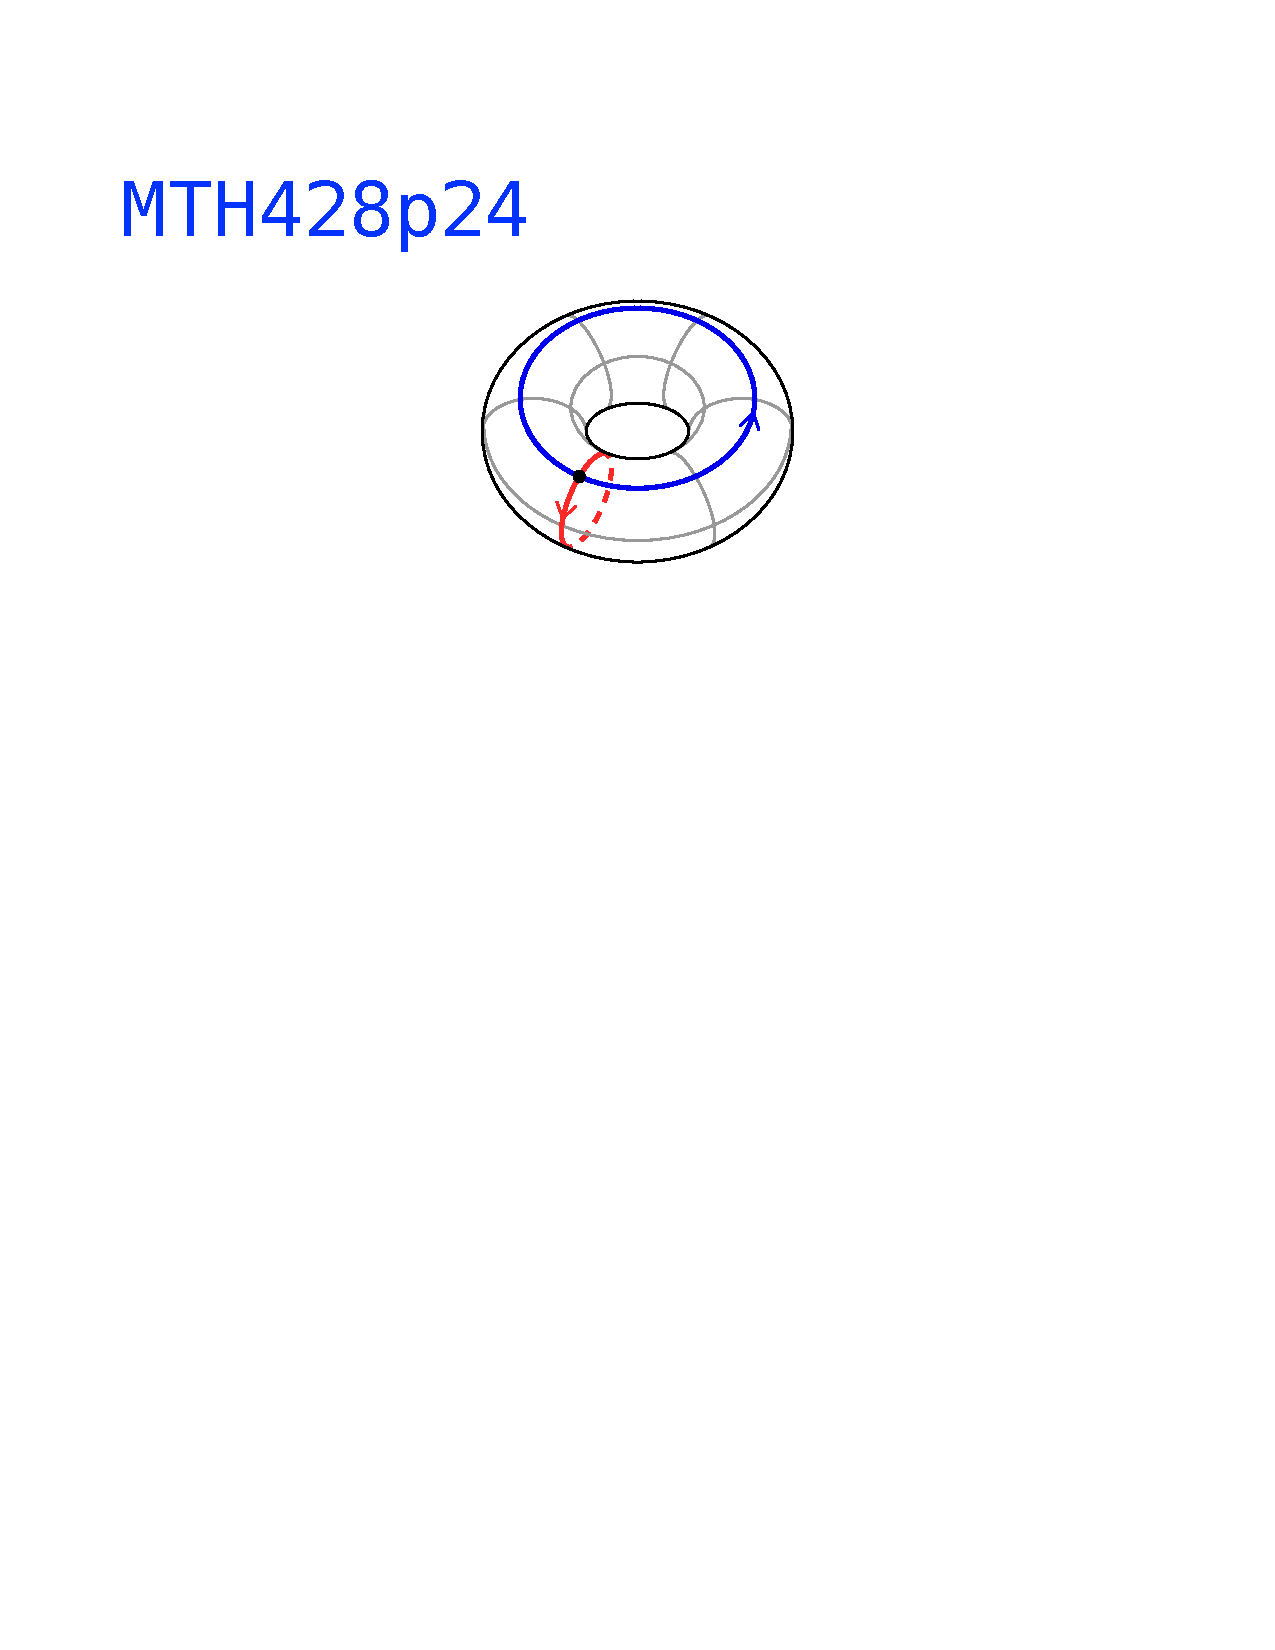
\includegraphics[width=\textwidth, trim=0mm 184mm 0mm 50mm, clip]{pictures/MTH428p024.pdf}}};

%%% COORDINATE GRID
%\draw[step=0.5, help lines] (0,0) to[grid with coordinates] (15,9);
%%% 

\end{tikzpicture}
\end{example}




Theorem \ref{PI1PROD THM} can be generalized to products of  arbitrary (finite or infinite)
families of spaces. Recall that if $\{G_{i}\}_{i\in I}$ is a family of groups then the direct product 
$\prod_{i\in I} G_{i}$ is the group whose set of elements is the Cartesian product of $G_{i}$'s 
with multiplication defined componentwise: $(g_{i})_{i\in I} \cdot (h_{i})_{i\in I} = (g_{i}h_{i})_{i\in I}$  

%---BBLANK # \newpage
\begin{theorem}
\label{PI1PRODGEN THM}
If ${(X_{i}, x_{i})}_{i\in I}$ is a family of pointed spaces then 
$$\pi_{1}\left(\prod_{i\in I} X_{i}, \ (x_{i})_{i\in I}\right) \cong  \prod_{i\in I} \pi_{1}(X_{i}, x_{i})$$
\end{theorem}
%---EBLANK # \vskip 30mm

The proof is the same as in the case of two spaces. 


Intuitively, one could rephrase Theorem \ref{PI1PRODGEN THM} by saying that the fundamental group 
takes products (of topological spaces) to products (of groups). It is possible to make this statement 
more precise by using the language of categories and functors. This starts with the following definition:

%---BBLANK
\begin{definition}
%---EBLANK # Categorical product definition. \end{definition}\newpage
\label{CATPROD DEF}
Let $\CC$ be a category and let $\{c_{i}\}_{i\in I}$ be a family of objects in $\CC$. 
The \emph{categorical product} of this family  is an object $d\in \CC$ equipped with 
a morphism $p_{i}\colon d \to c_{i}$
for each $i\in I $ and such that for any object $a$ and morphisms $f_{i}\colon a\to c_{i}$
there exists a unique morphism $g\colon a \to d$ satisfying 
$p_{i}g = f_{i}$ for all $i\in I$:
\begin{equation*}
\begin{tikzpicture}
\matrix (m) 
[matrix of math nodes, row sep=3em, column sep=3em, text height=1.5ex, text depth=0.25ex]
{
a &[-1em]     &                   \\[-1em]
   & d        &  c_{i}   \\
   & c_{j}  &             \\
};
\path[->, thick, font=\scriptsize]
(m-1-1) 
edge [bend left = 35] node[anchor = south west] {$f_{i}$} (m-2-3)
edge [bend right = 35] node[anchor = north east] {$f_{j}$} (m-3-2)
(m-2-2)
edge node[anchor = south] {$p_{i}$} (m-2-3)
edge node[anchor = east] {$p_{j}$} (m-3-2)
; 
\path[->, thick, dashed, font=\scriptsize]
(m-1-1)
edge node[auto] {$g$} (m-2-2)
;
\end{tikzpicture}
\end{equation*}

 
\end{definition}



\begin{example}
If $\{X_{i}\}_{i\in I}$ is a family of topological spaces then the product space $\prod_{i\in I} X_{i}$ 
together with the projection maps $p_{j}\colon \prod_{i\in I} X_{i} \to X_{j}$ given by 
$p_{j}((x_{i})_{i\in I}) = x_{j}$ is the categorical product of the family $\{X_{i}\}_{i\in I}$ 
in the category $\Top$ of topological spaces. 
Indeed, for any maps $f_{i}\colon Z \to X_{i}$ we have a map $g\colon Z \to \prod_{i\in I} X_{i}$ 
defined by $g(z) = (f_{i}(x))_{i\in I}$. Moreover $g$ is the unique map that satisfies $p_{i}g = f_{i}$
for all $i\in I$.
\end{example}

\begin{example}
Similarly as above one can  check that If $\{G_{i}\}_{i\in I}$ is a family of groups then the direct product 
$\prod_{i\in I} G_{i}$ taken together with the homomorphisms $p_{j}\colon \prod_{i\in I} G_{i} \to G_{j}$ 
given by $p_{j}((g_{i})_{i\in I}) = g_{j}$  is the categorical product of the family $\{G_{i}\}_{i\in I}$ in the 
category $\Gr$ of groups. 
\end{example}


\begin{note}
In general, in an arbitrary category $\CC$ categorical products may not exists. However, if 
a product of a family $\{c_{i}\}_{i\in I}$ exists then it is unique up to an isomorphism
(exercise). 
\end{note}

%---BBLANK
\begin{definition}
Let $F\colon \CC \to \CC'$ be a functor. Assume that $F$  has the property that  if  
an object $d$  with morphisms $p_{i}\colon d \to c_{i}$ is the categorical product of 
a family $\{c_{i}\}_{i\in I}$ in $\CC$ then the object $F(d)$ with morphisms 
$F(p_{i})\colon F(d) \to F(c_{i})$ is the categorical product of the family $\{F(c_{i})\}_{i\in I}$ 
in $\CC'$.  In such situation we say the  the functor $F$ \emph{preserves  products}. 
\end{definition}
%---EBLANK # \vskip 30mm

\begin{example}
Let $F\colon \Top \to \Gr$ be the functor such that $F(X) = \Z$ for each space $X$ and that 
for every map $f\colon X \to Y$ the homomorphism  $F(f)\colon F(X) \to F(Y)$ is the identity 
function $\id\colon \Z \to \Z$. The functor $F$ does not preserve products since for spaces 
$X, Y\in \Top$ we have 
$$F(X\times Y) = \Z  \ncong \Z \times \Z =  F(X)\times F(Y) $$
\end{example} 
 
In the category $\Top_{\ast}$ of pointed topological spaces the categorical products of 
a family  $\{(X_{i}, x_{i})\}_{i\in I}$ is given by the pointed space $(\prod_{i\in I}X_{i}, (x_{i})_{\in I})$.
In view of this Theorem \ref{PI1PRODGEN THM} can be restated as follows:

%---BBLANK
\begin{theorem}
The fundamental group functor $\pi_{1}\colon \Top_{\ast} \to \Gr$ preserves  products. 
\end{theorem}
%---EBLANK # \newpage



%%%%%%%%%%%%%%%%%%%%%%%%%%%%%%%
%  EXERCISES
%%%%%%%%%%%%%%%%%%%%%%%%%%%%%%%

\exercises

\begin{exercise}
The notion of a categorical coproduct is dual to the that of a product. Let $\CC$ be a category and  $\{c_{i}\}_{i\in I}$ be 
a family of objects in $\CC$. A \emph{coproduct} of this family  in the category $\CC$ is an object $d\in \CC$ equipped with  a morphism 
$h_{i}\colon c_{i} \to d$ for each $i\in I$  such that for any object $a$ and morphisms $f_{i}\colon  c_{i} \to a$
there exists a unique morphism $g\colon d \to a$ satisfying  $g h_{i} = f_{i}$ for all $i\in I$:
\begin{equation*}
\begin{tikzpicture}
\matrix (m) 
[matrix of math nodes, row sep=3em, column sep=3em, text height=1.5ex, text depth=0.25ex]
{
         &  c_{i}   &[-1.8em]             \\
c_{j}  &  d         &             \\[-1.8em]
         &             &      a      \\
};
\path[->, thick, font=\scriptsize]
(m-1-2) 
edge  node[anchor = west] {$h_{i}$} (m-2-2)
edge [bend left = 35] node[anchor = south west] {$f_{i}$} (m-3-3)
(m-2-1) 
edge node[anchor = north] {$h_{j}$} (m-2-2)
edge [bend right = 35] node[anchor = north east] {$f_{j}$} (m-3-3)
; 
\path[->, thick, dashed, font=\scriptsize]
(m-2-2)
edge node[anchor = south west] {$g$} (m-3-3)
;
\end{tikzpicture}
\end{equation*}

a) Let $\Ab$ denote the category of abelian groups (with abelian groups as objects and homomorphisms of abelian groups as morphisms). 
Show that if $\{G_{i}\}_{i\in I}$ is a family of abelian groups, then the direct sum $\bigoplus_{i\in I} G_{i}$ is the coproduct of this family in 
the category $\Ab$. 

b) Show that in the category $\Gr$ of all groups the direct sum $\Z\oplus\Z$ is not the coproduct of the family 
$\{\Z, \Z\}$.
\end{exercise}



\newpage
%%%%%%%%%%%%%%%%%%%%%%%%%%%%%%%
%%%%%%%%%%%%%%%%%%%%%%%%%%%%%%%
%%%
%%%  PUSHOUTS AND VAN KAMPEN'S THEOREM
%%%
%%%%%%%%%%%%%%%%%%%%%%%%%%%%%%%
%%%%%%%%%%%%%%%%%%%%%%%%%%%%%%%

%---BBLANK
\chapter[Pushouts and van Kampen's Theorem]{Pushouts \\ and  van Kampen's \\ Theorem}
%---EBLANK # \newpage
\chaptermark{Pushouts  and van Kampen's Theorem}

\thispagestyle{firststyle}
 
 Our main goal in this and the next chapter is  to explain and prove van Kampen's theorem, 
 which is one of the most useful tools for computing fundamental groups
 of spaces. This theorem says that if a space $(X, x_{0})$ can be decomposed into a union of two subspaces 
 $X  = U_{1}\cup U_{2}$ in a way that satisfies  a few conditions then it is possible to describe 
 $\pi_{1}(X, x_{0})$ in terms of the groups $\pi_{1}(U_{1}, x_{0})$, $\pi_{1}(U_{2}, x_{0})$, and 
 $\pi_{1}(U_{1}\cap U_{2}, x_{0})$. 
  
\begin{equation*}
\begin{tikzpicture}[scale = 0.6]
\fill[mygray1] (0,0) circle (2);
\fill[mygray1] (2.7, 0) circle (2);
\draw (0,0) circle (2);
\draw (2.7, 0) circle (2);
\draw[fill=black] ({2.7/2}, 0) node[anchor = south, outer sep = 2pt] {\small $x_{0}$} circle  (0.12);
\node[anchor= base]  at (-1.3 , 0){\small  $U_{1}$};
\node[anchor= base]  at ({2.7 + 1.3} , 0){\small  $U_{2}$};
\end{tikzpicture}
\end{equation*}
 
 
In Chapter \ref{PRODUCT FORMULA CHAPTER} we have 
 seen that the product formula for the fundamental group can be interpreted as a statement saying 
 that the functor $\pi_{1}\colon\Top_{\ast}\to \Gr$ preserves categorical products. Similarly, one way 
 to state van Kampen's  theorem is to say that under certain assumptions the functor $\pi_{1}$ preserves  
 categorical structures called \emph{pushouts}.  In this chapter we will discuss the notion of a pushout 
 in a general category. We will then describe how pushouts look like in the category of topological 
spaces and in the category of groups. This will allow us to state van Kampen's theorem precisely 
and show a few of its applications. The proof of this theorem  will be given in the next chapter.  
 
%---BBLANK 
 \begin{definition}
 %---EBLANK # Definition of a pushout. \end{definition}
Let $\CC$ be a category. Assume that we are given a diagram of objects and morphisms in $\CC$
of the following form:
\begin{equation*}
\begin{tikzpicture}
\matrix (m) 
[matrix of math nodes, row sep=3em, column sep=1.5em, text height=1.5ex, text depth=0.25ex]
{
c_{1} &  c_{0}   &  c_{2}       \\
};
\path[->, thick, font=\scriptsize]
(m-1-2) 
edge node[anchor = south] {$f_{1}$} (m-1-1)
edge node[anchor = south] {$f_{2}$} (m-1-3)
;
\end{tikzpicture}
\end{equation*}
A \emph{pushout} of this diagram is an object $p\in \CC$ equipped with morphisms 
$g_{i}\colon c_{i}\to p$ for $i=1, 2$ that satisfy the following conditions: 
\benu 
\item[1)] $g_{1}f_{1} = g_{2}f_{2}$
\item[2)] for any morphisms $h_{i}\colon c_{i}\to a$ ($i=1, 2$) that satisfy $h_{1}f_{1} = h_{2}f_{2}$
there exists a unique morphism $h\colon p\to a$ such that $hg_{i} =h_{i}$ for $i=1, 2$. 
\eenu
 
\begin{equation*}
\begin{tikzpicture}
\matrix (m) 
[matrix of math nodes, row sep=3em, column sep=3em, text height=1.5ex, text depth=0.25ex]
{
c_{0} &  c_{1}   &[-1.8em]             \\
c_{2} &  p         &             \\[-1.8em]
         &             &      a      \\
};
\path[->, thick, font=\scriptsize]
(m-1-1) 
edge node[anchor = south] {$f_{1}$} (m-1-2)
edge node[anchor = east] {$f_{2}$} (m-2-1)
(m-1-2) 
edge  node[anchor = west] {$g_{1}$} (m-2-2)
edge [bend left = 35] node[anchor = south west] {$h_{1}$} (m-3-3)
(m-2-1) 
edge node[anchor = north] {$g_{2}$} (m-2-2)
edge [bend right = 35] node[anchor = north east] {$h_{2}$} (m-3-3)
; 
\path[->, thick, dashed, font=\scriptsize]
(m-2-2)
edge node[anchor = south west] {$h$} (m-3-3)
;
\end{tikzpicture}
\end{equation*}
If such $p$ exists then we write 
$$
\begin{tikzpicture}[baseline = (m-1-1.base)]
\matrix (m) 
[matrix of math nodes, row sep=3em, column sep=2em, text height=1.5ex, text depth=0.25ex]
{
p = \colim(c_{1} &  c_{0}   &  c_{2})       \\
};
\path[->, thick, font=\scriptsize]
(m-1-2) 
edge node[anchor = south] {$f_{1}$} (m-1-1)
edge node[anchor = south] {$f_{2}$} (m-1-3)
;
\end{tikzpicture}
$$
 \end{definition}
 
 
\begin{note}
Pushout is a special instance of a more general notion of a \emph{colimit} (or a \emph{direct limit}). 
This is where the notation  $\colim$ comes from. 
\end{note} 
 
In a general category pushouts may not exist. However,  if a pushout of a 
diagram $c_{1} \la c_{0} \ra c_{2}$ exists then it is defined uniquely up to an isomorphism:

%---BBLANK #\vskip 90mm
\begin{proposition}
\label{PUSHOUT UNIQUE PROP}
Let $c_{1} \overset{f_{1}}{\la} c_{0} \overset{f_{2}}{\ra} c_{2}$ be a diagram in a category $\CC$
and let $p, p'\in \CC$.

1) If $p$ is a pushout of this diagram and $p' \cong p$ then $p'$ is also a pushout. 

2) Conversely, both  $p$ and $p'$ are pushouts of the above diagram then $p\cong p'$.  
\end{proposition}
%---EBLANK # \newpage 

\begin{proof}
Exercise. 
\end{proof}

\begin{note}
Proposition \ref{PUSHOUT UNIQUE PROP} shows that the notation $p = \colim(c_{1}\la c_{0}\to c_{2})$
is not entirely precise. It would be more accurate to write $p\cong \colim(c_{1} \la c_{0} \ra c_{2})$.
\end{note}



We will now look at constructions of pushouts in two categories that are of interests for us: the category 
of topological spaces and the category of groups.   

%---BBLANK
\textbf{Pushouts of topological spaces.} 
%---EBLANK # \vskip 10mm
Pushout is in the category $\Top$ can be described as follows:



%---BBLANK
\begin{proposition}
\label{TOP PUSHOUT PROP}
For any diagram of topological spaces 
$X_{1} \overset{f_{1}}{\la} X_{0} \overset{f_{2}}{\ra} X_{2}$
the pushout exists and it is given by 
\begin{equation*}
\begin{tikzpicture}[baseline = (m-1-1.base)]
\matrix (m) 
[matrix of math nodes, row sep=3em, column sep=1.5em, text height=1.5ex, text depth=0.25ex]
{
\colim(X_{1} &  X_{0}   &  X_{2})  = (X_{1}\sqcup X_{2})/{\sim}     \\
};
\path[->, thick, font=\scriptsize]
(m-1-2) 
edge node[anchor = south] {$f_{1}$} (m-1-1)
edge node[anchor = south] {$f_{2}$} (m-1-3)
;
\end{tikzpicture} 
\end{equation*}
where $\sim$ is the equivalence relation defined by $f_{1}(x) \sim f_{2}(x)$ for all $x\in X_{0}$. 
\end{proposition}

\begin{proof}
Exercise
\end{proof}
%---EBLANK


\begin{example}
Assume that $X_{0} = \varnothing$. We have $\colim(X_{1} \la \varnothing \ra X_{2}) = X_{1}\sqcup X_{2}$.\end{example}

\begin{example}
If $X$ is a space, $A\subseteq X$ is a subspace and   $\ast$ is a space consisting of one point 
then $\colim(\ast \la A \ra X) =  X /A$. 
\end{example}

\begin{example}
Recall that given a map $f\colon X \to Y$ by $M_{f}$ we denote the mapping cylinder of $f$ 
(\ref{MAP CYL CONE DEF}). We can view $M_{f}$ as a pushout as follows:
\begin{equation*}
\begin{tikzpicture}[baseline = (m-1-1.base)]
\matrix (m) 
[matrix of math nodes, row sep=3em, column sep=1.5em, text height=1.5ex, text depth=0.25ex]
{
M_{f} = \colim(Y &  X   &  X\times [0, 1])   \\
};
\path[->, thick, font=\scriptsize]
(m-1-2) 
edge node[anchor = south] {$f$} (m-1-1)
edge node[anchor = south] {$j$} (m-1-3)
;
\end{tikzpicture} 
\end{equation*}
where $j$ is given by $j(x) = (x, 1)$. 
\end{example}


%---BBLANK # \vskip 100mm
\begin{example}
\label{OPEN PUSHOUT EXAMPLE}
The following fact will be used later on. 
If $X$ is a topological space and $U, V\subseteq X$ are open sets such that 
$X= U\cup V$ then we have a homeomorphism 
\begin{equation*}
\begin{tikzpicture}
\matrix (m) 
[matrix of math nodes, row sep=3em, column sep=1.5em, text height=1.5ex, text depth=0.25ex]
{
X \cong \colim (U &  U\cap V   &  V)     \\
};
\path[->, thick, font=\scriptsize]
(m-1-2) 
edge  (m-1-1)
edge  (m-1-3)
;
\end{tikzpicture}
\end{equation*}
(exercise). Note that this is not true in general, if $U, V$ are not open in $X$. 
\end{example}
%---EBLANK # \newpage

%---BBLANK 
\textbf{Pushouts of groups.}  
%---EBLANK # \vskip 10mm
In the case of a diagram of topological spaces $X_{1}\la X_{0} \to X_{2}$
the pushout was constructed starting with the disjoint union $X_{1}\sqcup X_{2}$ and then performing
certain identifications in this space. Pushouts in the category of groups are built in a similar way, 
but the disjoint union of spaces is replaced by the free product of groups. We will describe 
free products first and then proceed to the construction of pushouts.  


%---BBLANK 
\begin{definition}
%---EBLANK # Free product  of groups $G\!\ast\! H$. \end{definition} \vskip 100mm
\label{FREE PROD GPS DEF}
The \emph{free product} of groups $G$ and $H$ is a group $G\!\ast\! H$ described as follows. 
\benu
\item[$\bullet$] Elements  of $G\!\ast\! H$ are sequences $(g_{1}, g_{2}, \dots,  g_{n})$ where $n\geq 0$ and $g_{i}\in G$  or $g_{i}\in H$ for each $i= 1, \dots, n$. 
\item[$\bullet$] If for some $i$ the elements $g_{i}, g_{i+1}$ are either both in $G$ or both in $H$ 
(so that we can take their product in one of these groups) then 
$$(g_{1}, \dots, g_{i} , g_{i+1}, \dots, g_{n}) = (g_{1}, \dots, g_{i}g_{i+1}, \dots, g_{n})$$ 
Also, if $g_{i}$ is the identity element in either $G$ or $H$ then 
$$(g_{1}, \dots, g_{i-1}, g_{i}, g_{i+1}, \dots, g_{n}) = (g_{1}, \dots, g_{i-1}, g_{i+1}, \dots, g_{n})$$ 
\item[$\bullet$] Multiplication in $G\!\ast\! H$ is defined by concatenation of sequences:
$$(g_{1}, \dots, g_{n})\cdot (g_{1}', \dots, g_{m}') = (g_{1}, \dots, g_{n}, g_{1}', \dots, g_{m}')$$
\eenu
\end{definition}


\begin{note}
Definition \ref{FREE PROD GPS DEF} can be extended to a free product of an arbitrary family 
$\{G_{j}\}_{j\in J}$ of groups. In this case the free product is the group $\ast_{j\in J} G_{j}$
whose elements are sequences $(g_{1}, g_{2}, \dots,  g_{n})$ where for each $i= 1, \dots, n$ 
we have $g_{i}\in G_{j}$ for some $j\in J$. Identities between such sequences and multiplication 
is defined analogously as in the case of two groups. 
\end{note}

\begin{note}
From now on we will write elements of $G\!\ast\! H$ as $g_{1}g_{2}\dots g_{n}$ instead of 
$(g_{1}, g_{2}, \dots,  g_{n})$. 
\end{note}

%---BBLANK 
\begin{proposition}
For any diagram of groups 
$G_{1}\overset{f_{1}}{\la} G_{0} \overset{f_{2}}{\ra} G_{2}$
the pushout exists and it is given by 
\begin{equation*}
\begin{tikzpicture}
\matrix (m) 
[matrix of math nodes, row sep=3em, column sep=1.5em, text height=1.5ex, text depth=0.25ex]
{
\colim (G_{1} &  G_{0}   &  G_{2})   = (G_{1}\! \ast \! G_{2})/N   \\
};
\path[->, thick, font=\scriptsize]
(m-1-2) 
edge node[anchor = south] {$f_{1}$} (m-1-1)
edge node[anchor = south] {$f_{2}$} (m-1-3)
;
\end{tikzpicture}
\end{equation*}
where $N$ is the normal subgroup of $G_{1}\!\ast\! G_{2}$ generated by all elements 
of the form $f_{1}(g)f_{2}(g)^{-1}$ for $g\in G_{0}$. 

\end{proposition}


\begin{proof}
Exercise.
\end{proof}
%---EBLANK  # \newpage

\begin{note} 
The group $(G_{1}\! \ast\! G_{2})/N$ described above is called the \emph{free amalgamated  product} of 
$G_{1}$ and $G_{2}$ and it is denoted by $G_{1}\!\ast_{G_{0}}\! G_{2}$
\end{note}

\begin{example}
Let $\{1\}$ denote the trivial group. We have $\colim(G_{1}\la \{1\} \ra G_{2}) = G_{1}\!\ast\!G_{2}$. 
\end{example}

\begin{example}
If $H$ is a  subgroup of $G$ then  $\colim(\{1\} \la H \ra G) = G/N$
where $N$ is the smallest normal  subgroup of $G$ generated by $H$. In particular 
is $H$ is a normal subgroup then $N= H$. 
\end{example}

We are now ready to state the main result of this chapter:

%---BBLANK 
\begin{VANKAMPENTHM}
\label{VANKAMPEN THM}
Let $(X, x_{0})$ be a pointed topological space and let $U_{1}, U_{2}\subseteq X$ be open sets such that 
$X = U_{1}\cup U_{2}$. 
If the sets $U_{1}$, $U_{2}$, and $U_{1}\cap U_{2}$ are path connected and $x_{0}\in U_{1}\cap U_{2}$ 
then 
\begin{equation*}
\begin{tikzpicture}[baseline = (m-1-1.base)]
\matrix (m) 
[matrix of math nodes, row sep=3em, column sep=2em, text height=1.5ex, text depth=0.25ex]
{
\pi_{1}(X, x_{0}) \cong \colim(\pi_{1}(U_{1}, x_{0}) &  \pi_{1}(U_{1}\cap U_{2}, x_{0})  &  \pi_{1}(U_{2}, x_{0}))     \\
};
\path[->, thick, font=\scriptsize]
(m-1-2) 
edge node[anchor = south] {$i_{1\ast}$} (m-1-1)
edge node[anchor = south] {$i_{2\ast}$} (m-1-3)
;
\end{tikzpicture} 
\end{equation*}
where for $k=1, 2$ the homomorphism $i_{k\ast}$ is induced by the inclusion map
$i_{k}\colon U_{1}\cap U_{2} \to U_{k}$. 
\end{VANKAMPENTHM}
%---EBLANK  # \newpage

\begin{note}
By Example \ref{OPEN PUSHOUT EXAMPLE}  under the assumptions of van Kampen's theorem 
we have a homeomorphism $X\cong \colim (U_{1} \la U_{1}\cap U_{2} \to U_{2})$. Thus van Kampen's theorem 
says that under some conditions the functor $\pi_{1}$ preserves pushouts:
\begin{equation*}
\begin{tikzpicture}[baseline = (m-1-1.base)]
\matrix (m) 
[matrix of math nodes, row sep=3em, column sep=1.3em, text height=1.5ex, text depth=0.25ex]
{
\pi_{1}(\colim(U_{1} &  
U_{1}\cap U_{2}  &  
U_{2}))  &[-1.8em] 
\ \cong\  &[-2em] 
\colim(\pi_{1}(U_{1}) &  
\pi_{1}(U_{1}\cap U_{2})  &  
\pi_{1}(U_{2}))     \\
};
\path[->, thick, font=\scriptsize]
(m-1-2) 
edge  (m-1-1)
edge  (m-1-3)
(m-1-6) 
edge  (m-1-5)
edge  (m-1-7)
;
\end{tikzpicture} 
\end{equation*}

\end{note}

We will now have a look at a few examples showing how van Kampen's Theorem can be used 
in computations of the fundamental group.

%---BBLANK  
\begin{example}
%---EBLANK  # $\pi_{1} (S^{1}\vee S^{1})$ \end{example} \newpage
\label{PI1S1VS1 EXAMPLE}
We will compute the fundamental group of the space $S^{1}\vee S^{1}$. It  will be convenient 
to choose as the basepoint of $S^{1}\vee S^{1}$ the point $x_{0}$ where the two copies of $S^{1}$ are
glued together:

\begin{equation*}
\begin{tikzpicture}[scale = 0.6]
\draw[line width = 1.6pt] (0,1) circle (1);
\draw[line width = 1.6pt] (0,-1) circle (1);
\draw[fill=black] (0,0) node[anchor = south] {\small $x_{0}$} circle (0.12);
\end{tikzpicture}
\end{equation*}

While $S^{1}\vee S^{1}$ is a union of two circles we cannot use these circles as
sets $U_{1}$ and $U_{2}$ in van Kampen's Theorem since they are not open in $S^{1}\vee S^{1}$. 
Instead we will decompose  $S^{1}\vee S^{1}$ as follows:

\begin{equation*}
\begin{tikzpicture}[scale = 0.6]
\draw[line width = 1.6pt] (0,1) circle (1);
\draw[line width = 1.6pt] (0,-1) circle (1);
\draw[fill=black] (0,0) circle (0.12);
\draw[line width = 1.4pt,  color = red, decorate, decoration={brace, amplitude = 5pt, mirror}] (-2, 2.086) -- (-2, -1) node [midway,xshift=-13pt]  {\small $\color{red} U_{1}$};
\draw[line width = 1.4pt,  color = myblue, decorate, decoration={brace, amplitude = 5pt}] (2, 1) -- (2, -2.086) node [midway,xshift=15pt]  {\small $\color{myblue} U_{2}$};
\draw[red, line width = 1.4pt, densely dotted] (-2,2.086) -- (1.8, 2.086) (-2, -1) -- (1.8, -1);
\draw[myblue, line width = 1.4pt, densely dotted] (2,1) -- (-1.8, 1) (2, -2.086) -- (-1.8, -2.086);
\end{tikzpicture}
\end{equation*}


Applying van Kampen's Theorem we obtain 
\begin{equation*}
\begin{tikzpicture}[baseline = (m-1-1.base)]
\matrix (m) 
[matrix of math nodes, row sep=3em, column sep=1.3em, text height=1.5ex, text depth=0.25ex]
{
\pi_{1}(S^{1}\vee S^{1}, x_{0}) \ \cong\  \colim(\pi_{1}(U_{1}, x_{0}) &  
\pi_{1}(U_{1}\cap U_{2}, x_{0})  &  \pi_{1}(U_{2}, x_{0}))     \\
};
\path[->, thick, font=\scriptsize]
(m-1-2) 
edge  (m-1-1)
edge  (m-1-3)
;
\end{tikzpicture} 
\end{equation*}
Notice that $U_{1}\simeq S^{1} \simeq U_{2}$ and and $U_{1}\cap U_{2} \simeq \ast$. It follows that 
$\pi(U_{1}, x_{0}) \cong \pi_{1}(U_{2}, x_{0})\cong \Z$ and $\pi_{1}(U_{1}\cap U_{2}, x_{0})\cong \{1\}$. 
This gives:
\begin{equation*}
\begin{tikzpicture}[baseline = (m-1-1.base)]
\matrix (m) 
[matrix of math nodes, row sep=0em, column sep=1.5em, text height=1.5ex, text depth=0.25ex]
{
\pi_{1}(S^{1}\vee S^{1}, x_{0}) \cong \colim(\Z &  \{1\}  &  \Z)  \cong \Z\!\ast\!\Z   \\
};
\path[->, thick, font=\scriptsize]
(m-1-2) 
edge  (m-1-1)
edge  (m-1-3)
;
\end{tikzpicture} 
\end{equation*}
Arguing by induction with respect to $n$ we obtain that 
$\pi_{1}(\bigvee_{i=1}^{n} S^{1}) \cong \ast_{i=1}^{n}\Z$.   
\end{example}


The following fact will be useful in the next example:

%---BBLANK 
\begin{lemma}
\label{CONTRACT VANKAMPEN LEMMA}
Let $X$ be a space and let $U_{1}, U_{2}\subseteq X$ be open sets such that $X = U_{1} \cup U_{2}$ 
and $U_{1}, U_{2}, U_{1}\cap U_{2}$
are path connected. If $\pi_{1}(U_{1})\cong \{1\}$ and $\pi_{1}(U_{2})\cong \{1\}$ then $\pi_{1}(X) \cong \{1\}$.  
\end{lemma}
%---EBLANK  #\vskip 80mm

\begin{proof}
Choose $x_{0}\in U_{1}\cap U_{2}$. By van Kampen's Theorem we get 
\begin{equation*}
\begin{tikzpicture}[baseline = (m-1-1.base)]
\matrix (m) 
[matrix of math nodes, row sep=3em, column sep=1.5em, text height=1.5ex, text depth=0.25ex]
{
\pi_{1}(X, x_{0}) \cong \colim( \{1\} &  \pi_{1}(U_{1}\cap U_{2}, x_{0})  &  \{1\} ) \cong \{1\}    \\
};
\path[->, thick, font=\scriptsize]
(m-1-2) 
edge  (m-1-1)
edge  (m-1-3)
;
\end{tikzpicture} 
\end{equation*}
\end{proof}

%---BBLANK 
\begin{example}
%---EBLANK # $\pi_{1}(S^{n})$ \end{example} \newpage
\label{PI1 SN TRIVIAL EXAMPLE}
Take a sphere $S^{n}$, $n> 1$. Let $x_{0}\in S^{n}$ be a basepoint, and let $x_{1}, x_{2}$ be two points 
distinct from $x_{0}$:

\begin{tikzpicture}

\node[anchor=south west,inner sep=0] at (0,0) 
{{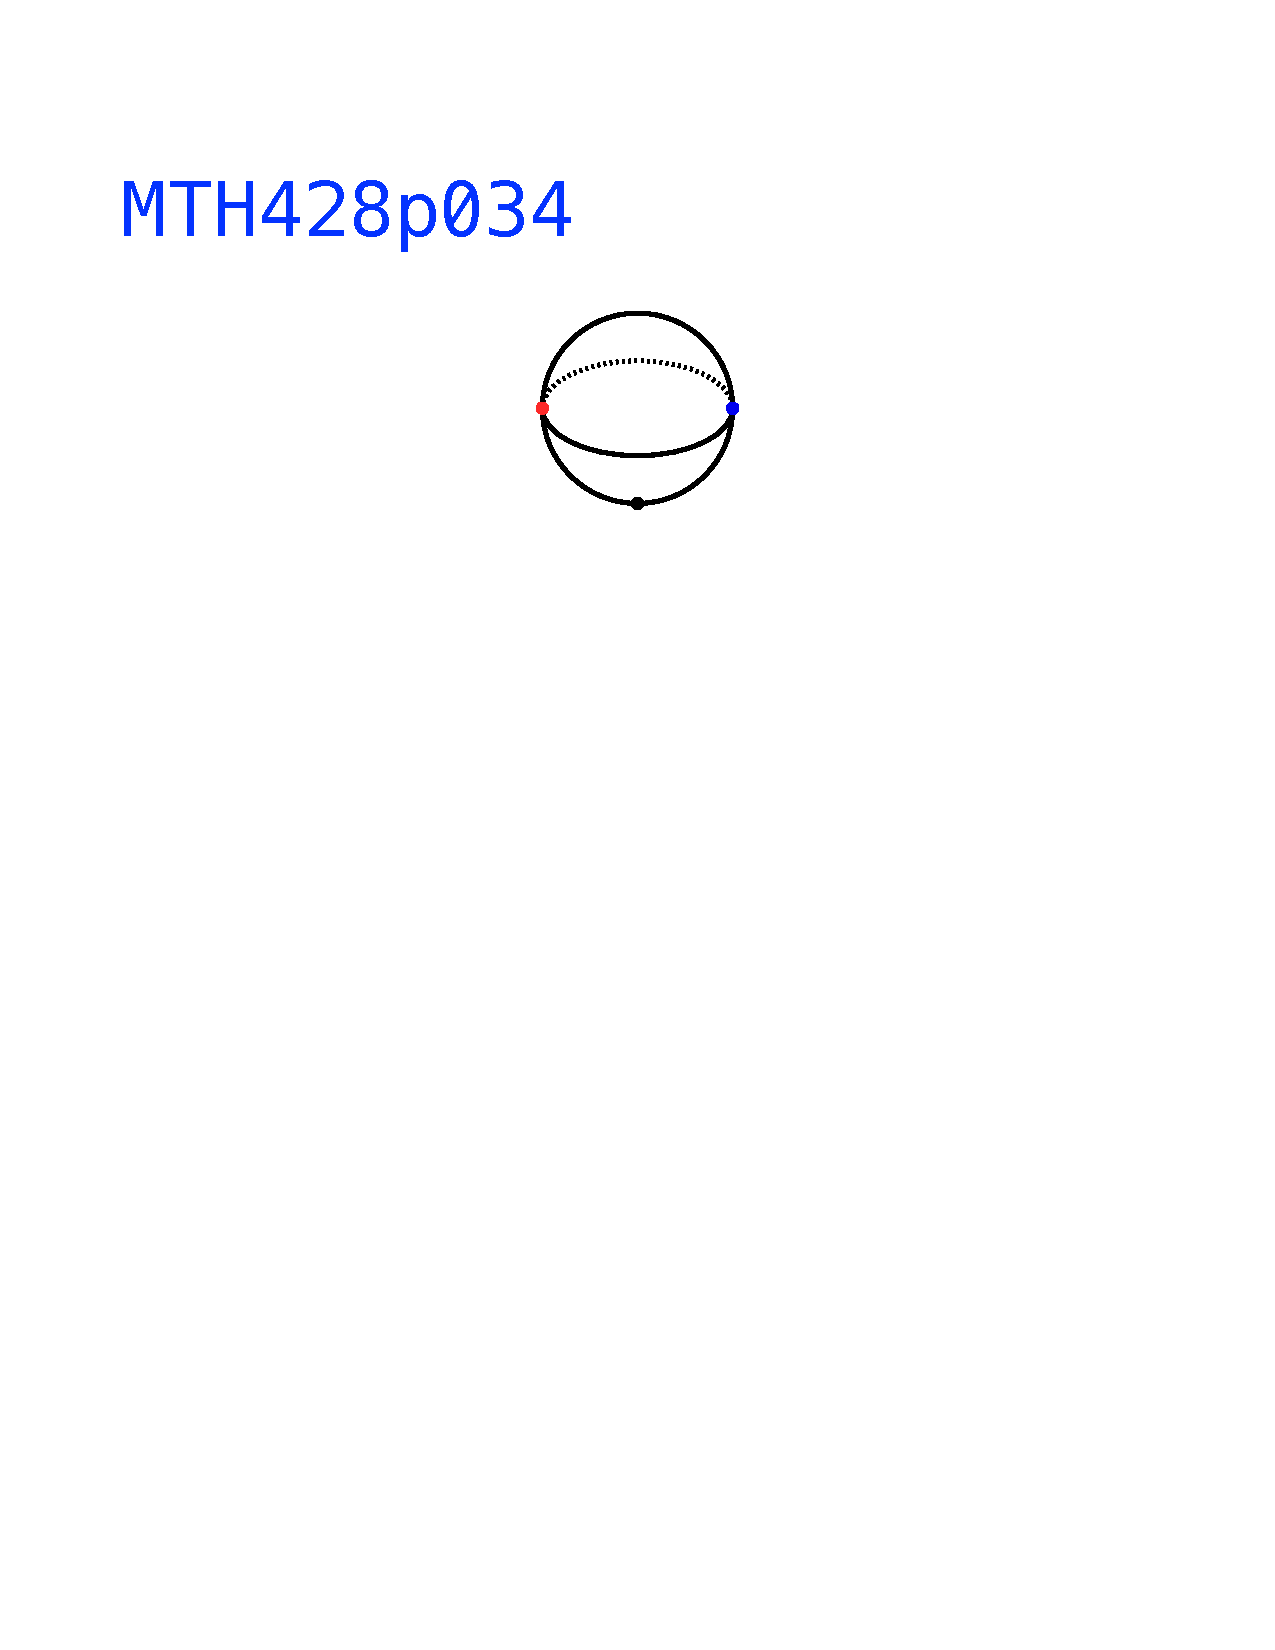
\includegraphics[width=\textwidth, trim=0mm 192mm 0mm 52mm, clip]{pictures/MTH428p034.pdf}}};

%%% COORDINATE GRID
%\draw[step=0.5, help lines] (0,0) to[grid with coordinates] (15,9);
%%% 

\node[anchor= base east]  at (7.0 , 1.32){\color{red} \small  $x_{1}$};
\node[anchor= base west]  at (9.52 , 1.32){\color{blue} \small  $x_{2}$};
\node[anchor= north]  at (8.3 , 0.1){\small  $x_{0}$};
\end{tikzpicture}

Take $U_{1}= S^{n}\ssmin\{x_{1}\}$,  $U_{2}= S^{n}\ssmin \{x_{2}\}$. 
We have $U_{1}\cong \R^{n}\cong U_{2}$, 
and so $\pi_{1}(U_{1}, x_{0})\cong \pi_{1}(U_{2}, x_{0})\cong \{1\}$. By Proposition 
\ref{CONTRACT VANKAMPEN LEMMA} we obtain that $\pi_{1}(S^{n}, x_{0})\cong \{1\}$ for $n>1$. 
\end{example}


%%%%%%%%%%%%%%%%%%%%%%%%%%%%%%%
%  EXERCISES
%%%%%%%%%%%%%%%%%%%%%%%%%%%%%%%

\exercises

\begin{exercise}
Prove Proposition \ref{PUSHOUT UNIQUE PROP}
\end{exercise}

\begin{exercise}
Assume that we have the following commutative diagram in a category $\CC$:
\begin{equation*}
\begin{tikzpicture}[baseline=(current  bounding  box.center)]
\matrix (m) 
[matrix of math nodes, row sep=3em, column sep=3em, text height=1.5ex, text depth=0.25ex]
{
c_{1} & c_{0} & c_{2}  \\
c'_{1} & c'_{0} & c'_{2}  \\
};
\path[->, thick, font=\scriptsize]
(m-1-1) 
edge node[anchor = east] {$g_{1}$} (m-2-1)
(m-1-2) 
edge node[anchor = south] {$f_{1}$} (m-1-1)
edge node[anchor = south] {$f_{2}$} (m-1-3)
edge node[anchor = east] {$g_{0}$} (m-2-2)
(m-1-3) 
edge node[anchor = west] {$g_{2}$} (m-2-3)
(m-2-2) 
edge node[anchor = north] {$f'_{1}$} (m-2-1)
edge node[anchor = north] {$f'_{2}$} (m-2-3)
;
\end{tikzpicture}
\end{equation*}
Show that if the morphisms $g_{0}, g_{1}, g_{2}$ are isomorphisms, then there exists an isomorphism 
$$
\begin{tikzpicture}[baseline = (m-1-1.base)]
\matrix (m) 
[matrix of math nodes, row sep=3em, column sep=2em, text height=1.5ex, text depth=0.25ex]
{
\colim(c_{1} &  c_{0}   &  c_{2})    &   &  \colim(c'_{1} &  c'_{0}   &  c'_{2})   \\
};
\path[->, thick, font=\scriptsize]
(m-1-2) 
edge node[anchor = south] {$f_{1}$} (m-1-1)
edge node[anchor = south] {$f_{2}$} (m-1-3)
(m-1-6) 
edge node[anchor = south] {$f'_{1}$} (m-1-5)
edge node[anchor = south] {$f'_{2}$} (m-1-7)
(m-1-3) 
edge[shorten <=2mm, shorten >=2mm] node[anchor = south] {$\cong$} (m-1-5)
;
\end{tikzpicture}
$$


\end{exercise}



\begin{exercise}
Prove Proposition \ref{TOP PUSHOUT PROP}.
\end{exercise}

\begin{exercise}
Let $X$ be a topological space, and let $U, V \subseteq X$ be sets such that $U\cup V = X$. 

a) Show that if $U$ and $V$ are open sets then there exists a homeomorphism 
\begin{equation*}
\begin{tikzpicture}
\matrix (m) 
[matrix of math nodes, row sep=3em, column sep=1.5em, text height=1.5ex, text depth=0.25ex]
{
X \cong \colim (U &  U\cap V   &  V)     \\
};
\path[->, thick, font=\scriptsize]
(m-1-2) 
edge  (m-1-1)
edge  (m-1-3)
;
\end{tikzpicture}
\end{equation*}
b) Give an example of a space $X$ and (non-open) sets $U, V \subseteq X$ such that 
the above homeomorphism does not hold.  Justify your answer. 
\end{exercise}








\begin{exercise}
Let $U, V$ be open sets in $\R^{n}$ such that 
$U, V, U\cap V$ are path connected, and $U\cup V = \R^{n}$. Let $x_{0}\in U\cap V$. 
Show that if $\pi_{1}(U, x_{0})\not \cong\{1\}$  then $\pi_{1}(U\cap V, x_{0}) \not \cong \{1\}$. 
\end{exercise}



\begin{exercise}
Compute the fundamental group of each of the following spaces.

a)  The space $X_{1}$ obtained from $\R^{3}$ by removing  $n$ straight lines 
intersecting at the origin.

b) The space $X_{2}$ obtained from $\R^{3}$ by removing  the circle 
$$S^{1}=\{(x, y, z)\in \R^{3} \ | \ x^{2}+y^{2}=1, \ z=0 \}$$
and the $z$-axis.

c)  The space $X_{3}$ obtained from two copies of the 
torus $S^{1}\times S^{1}$ by identifying the circle $S^{1}\times \{x_{0}\}$ in one torus 
with the circle $\{x_{0}\}\times S^{1}$ in the other torus. 

d) The space $X_{4}$ obtained by removing a straight line from $\R^{4}$. 

e) The space $X_{5}$ obtained by removing a 2-dimensional vector subspace from $\R^{4}$.
\end{exercise}




\begin{exercise}
Let $S^{3}$ be the 3-dimensional sphere, let $A\subset S^{3}$ be a closed subspace of 
$S^{3}$, and let $x_{0}\in S^{3}$.  Assuming that the space  $S^{3}-(A\cup \{x_{0}\})$
is path connected show that the inclusion map 
$$j\colon S^{3}- (A\cup \{x_{0}\})\hookrightarrow S^{3}- A$$
induces an isomorphism of  fundamental groups.
\end{exercise}






\begin{exercise}
Let $f\colon X \to Y_{1}$ and $g\colon X \to Y_{2}$ be maps of topological spaces. The \emph{double mapping cylinder}
of $f$ and $g$ is the space
$$M(f, g) = ( Y_{1} \sqcup X \times [0, 1] \sqcup Y_{2}) /{\sim}$$
where $\sim$ is the equivalence relation given by $(x, 0)\sim f(x)$ and $(x, 1)\sim g(x)$ for all $x\in X$.  
Show that if $X, Y_{1}, Y_{2}$ are path connected spaces and $x_{0}\in X$ then there exists an isomorphism
\begin{equation*}
\begin{tikzpicture}[baseline = (m-1-1.base)]
\matrix (m) 
[matrix of math nodes, row sep=3em, column sep=2em, text height=1.5ex, text depth=0.25ex]
{
\pi_{1}(M(f, g)) \cong \colim(\pi_{1}(Y_{1}, f(x_{0})) &  \pi_{1}(X, x_{0}) &  \pi_{1}(Y_{2}, g(x_{0})))     \\
};
\path[->, thick, font=\scriptsize]
(m-1-2) 
edge node[anchor = south, pos=0.4] {$f_{\ast}$} (m-1-1)
edge node[anchor = south] {$g_{\ast}$} (m-1-3)
;
\end{tikzpicture} 
\end{equation*}
\end{exercise}


\begin{exercise}
The \emph{join} of  spaces  $X$ and $Y$ is the space $X \ast Y$ given by 
$$X \ast Y = X \times Y \times [0, 1] /{\sim}$$
where $(x, y, 0)\sim (x, y', 0)$ for all $x\in X$, $y, y'\in Y$, and 
$(x, y, 1)\sim (x', y, 1)$ for all $x, x'\in X$, $y \in Y$.  Show that if $X$ and $Y$ are non-empty path connected 
spaces then $\pi_{1}(X\ast Y) \cong \{1\}$.
\end{exercise}




\begin{exercise}
Recall that a topological group is a topological space $X$ equipped with a group structure such that 
the maps $\mu\colon X\times X\to X$, $\mu(g, h) = gh$ and $\eta\colon X \to X$, $\eta(g) = g^{-1}$ are continuous. 
For example, the space $\R^{2}$ is a topological group with the addition 
$$(x, y) + (x', y') = (x+ x', y +y')$$ 
defining the group structure. 

a) Show that for any $x_{1}\in \R^{2}$ the space $X = \R^{2}\ssmin \{x_{1}\}$ can be given the structure of 
a topological group. 

b) Show that for $n >1$  the space $X = \R^{2}\ssmin \{x_{1}, \dots, x_{n}\}$ does not have the structure 
of a topological group. 
\end{exercise}








\newpage
%%%%%%%%%%%%%%%%%%%%%%%%%%%%%%%
%%%%%%%%%%%%%%%%%%%%%%%%%%%%%%%
%%%
%%%  PROOF OF VAN KAMPEN'S THEOREM
%%%
%%%%%%%%%%%%%%%%%%%%%%%%%%%%%%%
%%%%%%%%%%%%%%%%%%%%%%%%%%%%%%%


%---BBLANK 
\chapter[Proof of van Kampen's Theorem]{Proof of  \\ van Kampen's \\ Theorem}
%---EBLANK 
\chaptermark{Proof of van Kampen's Theorem}

\thispagestyle{firststyle}


In the last chapter have seen the statement of van Kampen's theorem and some of examples of its
applications. Our main goal in this chapter is to prove this result. For reference we 
state it here again:

%---BBLANK 
{
\renewcommand{\thetheorem}{\ref{VANKAMPEN THM}}
\begin{VANKAMPENTHM}
Let $(X, x_{0})$ be a pointed topological space and let $U_{1}, U_{2}\subseteq X$ be open sets such that 
$X = U_{1}\cup U_{2}$. 
If  the sets $U_{1}$, $U_{2}$, and $U_{1}\cap U_{2}$ are path connected and $x_{0}\in U_{1}\cap U_{2}$ 
then 
\begin{equation*}
\begin{tikzpicture}[baseline = (m-1-1.base)]
\matrix (m) 
[matrix of math nodes, row sep=3em, column sep=1.5em, text height=1.5ex, text depth=0.25ex]
{
\pi_{1}(X, x_{0}) \cong \colim(\pi_{1}(U_{1}, x_{0}) &  \pi_{1}(U_{1}\cap U_{2}, x_{0})  &  \pi_{1}(U_{2}, x_{0}))     \\
};
\path[->, thick, font=\scriptsize]
(m-1-2) 
edge node[anchor = south] {$i_{1\ast}$} (m-1-1)
edge node[anchor = south] {$i_{2\ast}$} (m-1-3)
;
\end{tikzpicture} 
\end{equation*}
where for $k=1, 2$ the homomorphism $i_{k\ast}$ is induced by the inclusion map
$i_{k}\colon U_{1}\cap U_{2} \to U_{k}$. 
\end{VANKAMPENTHM}
\addtocounter{theorem}{-1}
}
%---EBLANK  #\newpage

%---BBLANK 
%---EBLANK  #\ \newpage \ \newpage

\begin{proof}
Here is some notation that will be useful. 
\benu
\item[\textbullet]  For simplicity we will denote $U_{1}\cap U_{2}$ by $U_{0}$. 
\item[\textbullet] For $k=1, 2$ by  $i_{k}\colon U_{0}\to U_{k}$ and $j_{k}\colon U_{k}\to X$  
we will denote the inclusion maps. 
\item[\textbullet] If $\omega$ is a loop in $U_{1}$ then it represents an element 
of $\pi_{1}(U_{1}, x_{0})$ and an element of $\pi_{1}(X, x_{0})$. In order to avoid such ambiguities we will 
write $[\omega]_{k}$ to indicate an element of $\pi_{1}(U_{k}, x_{0})$ and $[\omega]$ to indicate 
an element of $\pi_{1}(X, x_{0})$.   
\eenu
The strategy of the proof will be as follows. Let 
$P = \colim(\pi_{1}(U_{1}, x_{0}) \overset{i_{1\ast}}\la 
\pi_{1}(U_{0}, x_{0}) \overset{i_{2\ast}}{\to} \pi_{1}(U_{2}, x_{0}))$. 
Recall that by Proposition \ref{PUSHOUT UNIQUE PROP}
$P$ is the unique (up to an isomorphism) group that satisfies the following conditions:
\benu
\item[1)] for $k=1, 2$ there exists exists a homomorphism $g_{k}\colon \pi_{1}(U_{k}, x_{0}) \to P$
such that $g_{1}i_{1\ast} = g_{2}i_{\ast}$; 
\item[2)] for any group  $G$ and any homomorphisms $h_{k}\colon \pi_{1}(U_{k}, x_{0}) \to P$
satisfying  $h_{1}i_{1\ast} = h_{2}i_{\ast}$ there exists a unique homomorphism $h\colon P\to G$
such that $hg_{k} = h_{k}$ for $k=1, 2$.
%\begin{equation*}
%\begin{tikzpicture}
%\matrix (m) 
%[matrix of math nodes, row sep=3em, column sep=2em, text height=1.5ex, text depth=0.25ex]
%{
%\pi_{1}(U_{0}, x_{0}) &  \pi_{1}(U_{1}, x_{0})   &[-1.5em]             \\
%\pi_{1}(U_{2}, x_{0}) &  P         &             \\[-1.5em]
%         &             &      G      \\
%};
%\path[->, thick, font=\scriptsize]
%(m-1-1) 
%edge node[anchor = south] {$i_{1\ast}$} (m-1-2)
%edge node[anchor = east] {$i_{2\ast}$} (m-2-1)
%(m-1-2) 
%edge  node[anchor = west] {$g_{1}$} (m-2-2)
%(m-1-2.350) 
%edge [bend left = 35] node[anchor = south west] {$h_{1}$} (m-3-3)
%(m-2-1) 
%edge node[anchor = north] {$g_{2}$} (m-2-2)
%edge [bend right = 35] node[anchor = north east] {$h_{2}$} (m-3-3)
%; 
%\path[->, thick, dashed, font=\scriptsize]
%(m-2-2)
%edge node[anchor = south west] {$h$} (m-3-3)
%;
%\end{tikzpicture}
%\end{equation*}
\eenu   
If follows that in order to prove van Kampen's theorem it will suffice to show
that the group $\pi_{1}(X, x_{0})$ satisfies conditions 1) and 2). The first condition is satisfied
by taking $g_{k} = j_{k\ast}$ for $k=1, 2$. In order to verify the second condition let 
$h_{1}\colon \pi_{1}(U_{1}, x_{0}) \to G$ and 
$h_{2}\colon \pi_{1}(U_{2}, x_{0}) \to G$ be 
homomorphisms satisfying $h_{1}i_{1\ast} = h_{2}i_{2\ast}$. We need to construct a homomorphism 
$h\colon \pi_{1}(X, x_{0})\to G$ such that the following diagram commutes:
\begin{equation*}
\label{VANK PUSHOT EQ}
\tag{$\ast$}
\begin{tikzpicture}[baseline=(current  bounding  box.center)]
\matrix (m) 
[matrix of math nodes, row sep=3em, column sep=2em, text height=1.5ex, text depth=0.25ex]
{
\pi_{1}(U_{0}, x_{0}) &  \pi_{1}(U_{1}, x_{0})   &[-1.5em]             \\
\pi_{1}(U_{2}, x_{0}) &  \pi_{1}(X, x_{0})         &             \\[-1.5em]
         &             &      G      \\
};
\path[->, thick, font=\scriptsize]
(m-1-1) 
edge node[anchor = south] {$i_{1\ast}$} (m-1-2)
edge node[anchor = east] {$i_{2\ast}$} (m-2-1)
(m-1-2) 
edge  node[anchor = west] {$j_{1\ast}$} (m-2-2)
(m-1-2.350) 
edge [bend left = 35] node[anchor = south west] {$h_{1}$} (m-3-3)
(m-2-1) 
edge node[anchor = north] {$j_{2\ast}$} (m-2-2)
edge [bend right = 35] node[anchor = north east] {$h_{2}$} (m-3-3)
; 
\path[->, thick, dashed, font=\scriptsize]
(m-2-2)
edge node[anchor = south west] {$h$} (m-3-3)
;
\end{tikzpicture}
\end{equation*}
Moreover, we need to show that there is only one such homomorphism $h$. 

The construction of $h$  will use the following setup. For each point $x\in X$ 
choose a path $\sigma_{x}$ such that
\benu
\item[\textbullet]  $\sigma_{x}(0) =  x$ and $\sigma_{x}(1) = x_{0}$; 
\item[\textbullet] if $x\in U_{k}$ for  $k\in \{0, 1, 2\}$ then $\sigma_{x}$ is contained in $U_{k}$;
\item[\textbullet] $\sigma_{x_{0}}$  is the constant path.  
\eenu
Such paths exist since by assumption $U_{0}, U_{1}, U_{2}$ are path connected sets. 
If $\omega$ is a path in $X$ then the concatenation 
$\xov{\sigma}_{\omega(0)} \ast \omega \ast \sigma_{\omega(1)}$ is a loop based at $x_{0}$:

\begin{tikzpicture}

\node[anchor=south west,inner sep=0] at (0,0) 
{{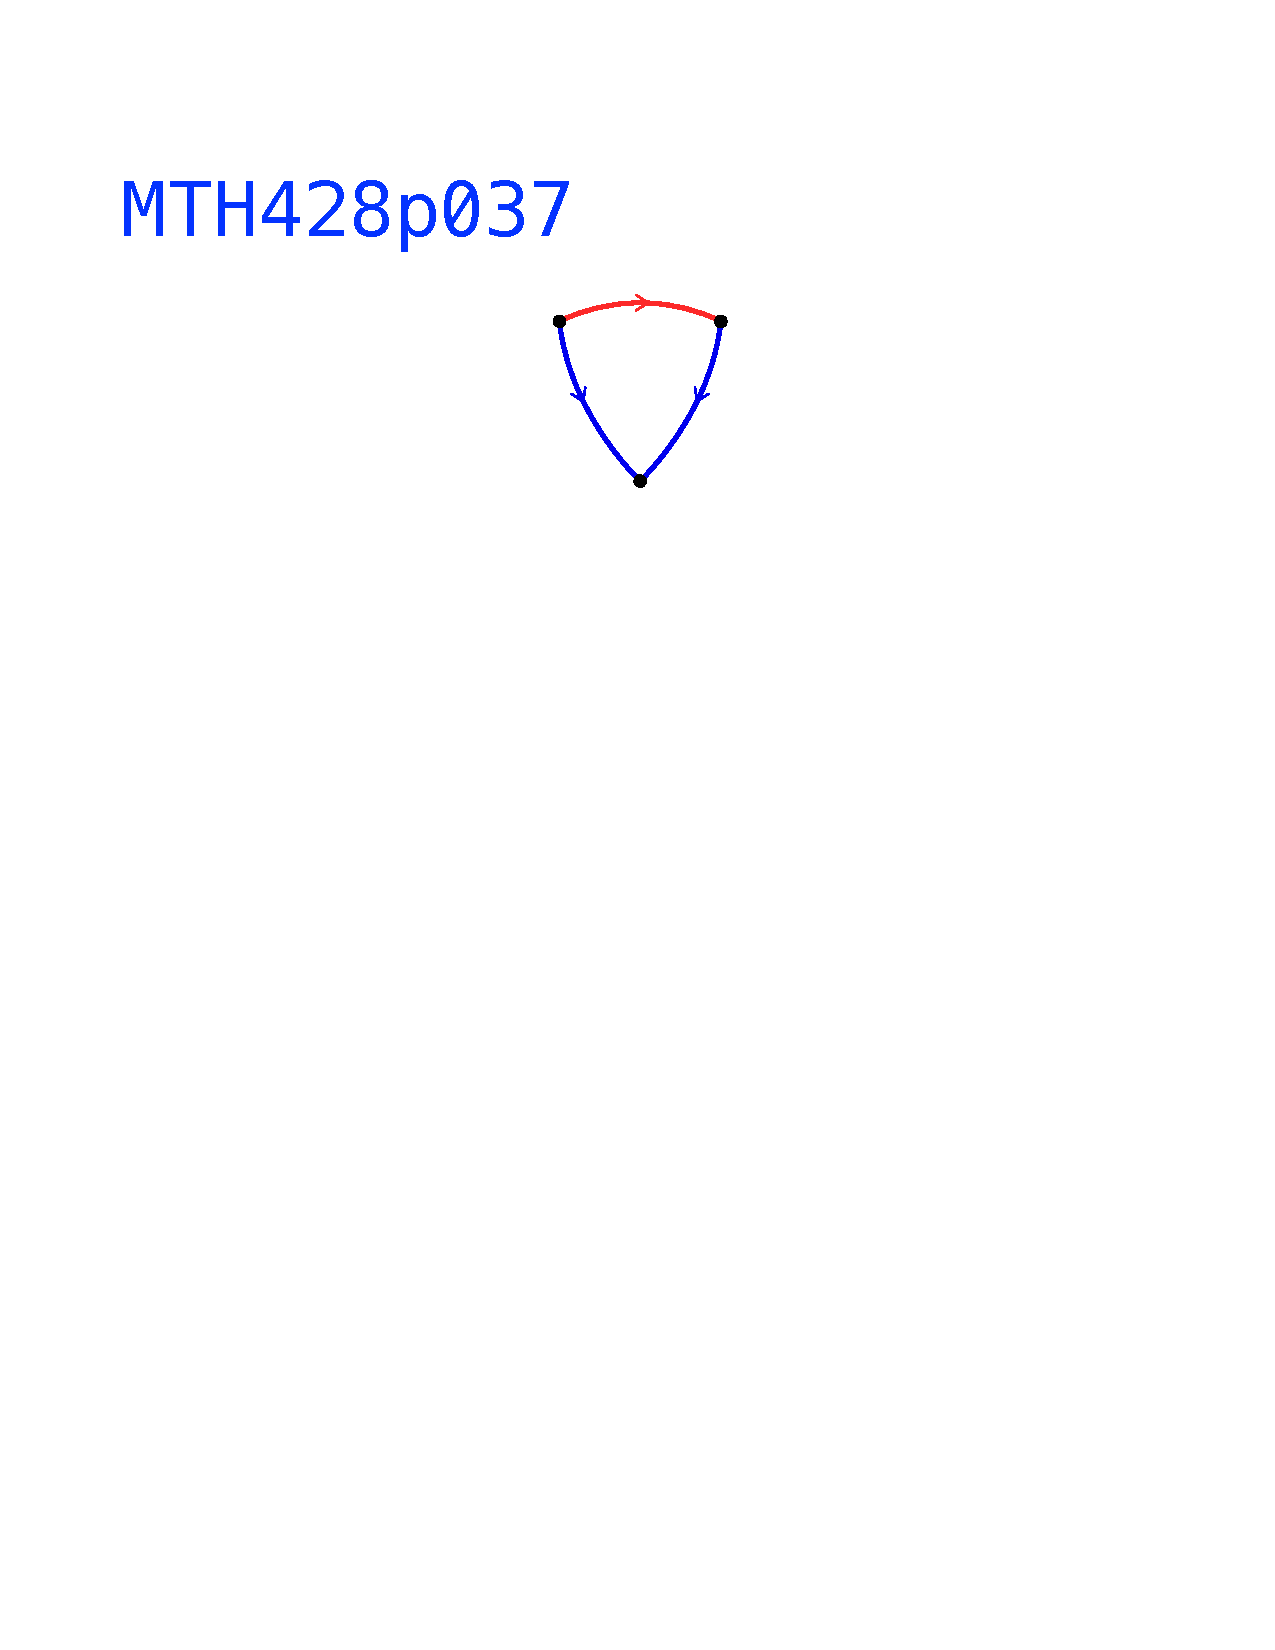
\includegraphics[width=\textwidth, trim=0mm 196mm 0mm 49mm, clip]{pictures/MTH428p037.pdf}}};

%%% COORDINATE GRID
%\draw[step=0.5, help lines] (0,0) to[grid with coordinates] (15,9);
%%% 

\node[anchor= base]  at (8.35 , -0.23){\small  $x_{0}$};
\node[anchor= base]  at (8.33 , 2.65){\color{red} \small  $\omega$};
\node[anchor= base]  at (6.98 , 1.2){\color{blue} \small  $\sigma_{\omega(0)}$};
\node[anchor= base]  at (9.63 , 1.2){\color{blue} \small  $\sigma_{\omega(1)}$};

\end{tikzpicture}

 We will denote this loop by $\omega^{\circ}$ and call it the \emph{loop completion} of $\omega$.
Loop completion has the following properties:
\benu
 \item[(i)] If $\omega$ is a path in $U_{k}$ for $k\in \{0, 1, 2\}$ then $\omega^{\circ}$ is a loop in $U_{k}$.
This holds since in such case $\sigma_{\omega(0)}$ and $\sigma_{\omega(1)}$ are paths in $U_{k}$. 
\item[(ii)] For any path $\omega$ we have $(\xov{\omega})^{\circ} \simeq \xov{\omega^{\circ}}$. 
\item[(iii)] If $\omega$, $\tau$ have the same endpoints and $\omega\simeq \tau$ then 
$\omega^{\circ} \simeq \tau^{\circ}$, and so in $\pi_{1}(X, x_{0})$ we have $[\omega^{\circ}] = [\tau^{\circ}]$. Moreover, if $\omega$, $\tau$ are paths in $U_{k}$ and the homotopy between them is contained in 
$U_{k}$ then in $\pi_{1}(U_{k}, x_{0})$ we have $[\omega^{\circ}]_{k} = [\tau^{\circ}]_{k}$.
 \item[(iv)]  If $\omega, \tau$ are paths such that $\omega(1) = \tau(0)$ then  
 $(\omega\ast\tau)^{\circ} \simeq \omega^{\circ}\ast\tau^{\circ}$.
 Indeed, we have 
$$\omega^{\circ}\ast\tau^{\circ} = (\xov{\sigma}_{\omega(0)}\ast \omega \ast
\sigma_{\omega(1)})\ast 
(\xov{\sigma}_{\omega(1)}\ast \tau \ast \sigma_{\tau(1)})
\simeq \xov{\sigma}_{\omega(0)}\ast \omega\ast\tau \ast \sigma_{\tau(1)} \simeq (\omega\ast\tau)^{\circ}$$
Notice also that if both $\omega$ and $\tau$ are paths in $U_{k}$ then the above homotopy of loops is contained in $U_{k}$. This means that $[\omega^{\circ}]_{k} \cdot  [\tau^{\circ}]_{k} =  [(\omega\ast\tau)^{\circ}]_{k}$ 
in $\pi_{1}(U_{k}, x_{0})$.  
\item[(v)] If $\omega$ is a loop based at $x_{0}$ then $\omega \simeq \omega^{\circ}$. To see this notice 
that in this case $\sigma_{\omega(0)} = \sigma_{\omega(1)} = \sigma_{x_{0}}$, and by assumption 
$ \sigma_{x_{0}}$ is the constant path. 
Therefore we have $\omega^{\circ} = \xov{\sigma}_{x_{0}}\ast \omega \ast \sigma_{x_{0}} \simeq \omega$. 

 \eenu
 
We are now ready to describe the construction of the homomorphism $h$ in the diagram
(\ref{VANK PUSHOT EQ}). Let $\omega \colon [0, 1]\to X$ be a loop. The sets 
$\omega^{-1}(U_{1})$ and $\omega^{-1}(U_{2})$ 
form an open cover of the interval $[0, 1]$. Using the Lebesgue number of  this cover we
obtain that there exists an $n$-tuple of numbers $(s_{0},  \dots, s_{n})$ such that  
$0=s_{0} < s_{1} < {\dots} < s_{n} = 1$ and  $\omega([s_{i-1}, s_{i}])$ is contained in either 
$U_{1}$ or $U_{2}$ for each $i=1, \dots, n$. 
Let $\omega_{i}\colon [0, 1]\to X$ be the path given by $\omega_{i}(s) = \omega(s_{i-1}s + s_{i}(1-s))$. 
This path coincides with the restriction of $\omega$ to the subinterval $[s_{i-1}\colon s_{i}]$:

\begin{tikzpicture}

\node[anchor=south west,inner sep=0] at (0,0) 
{{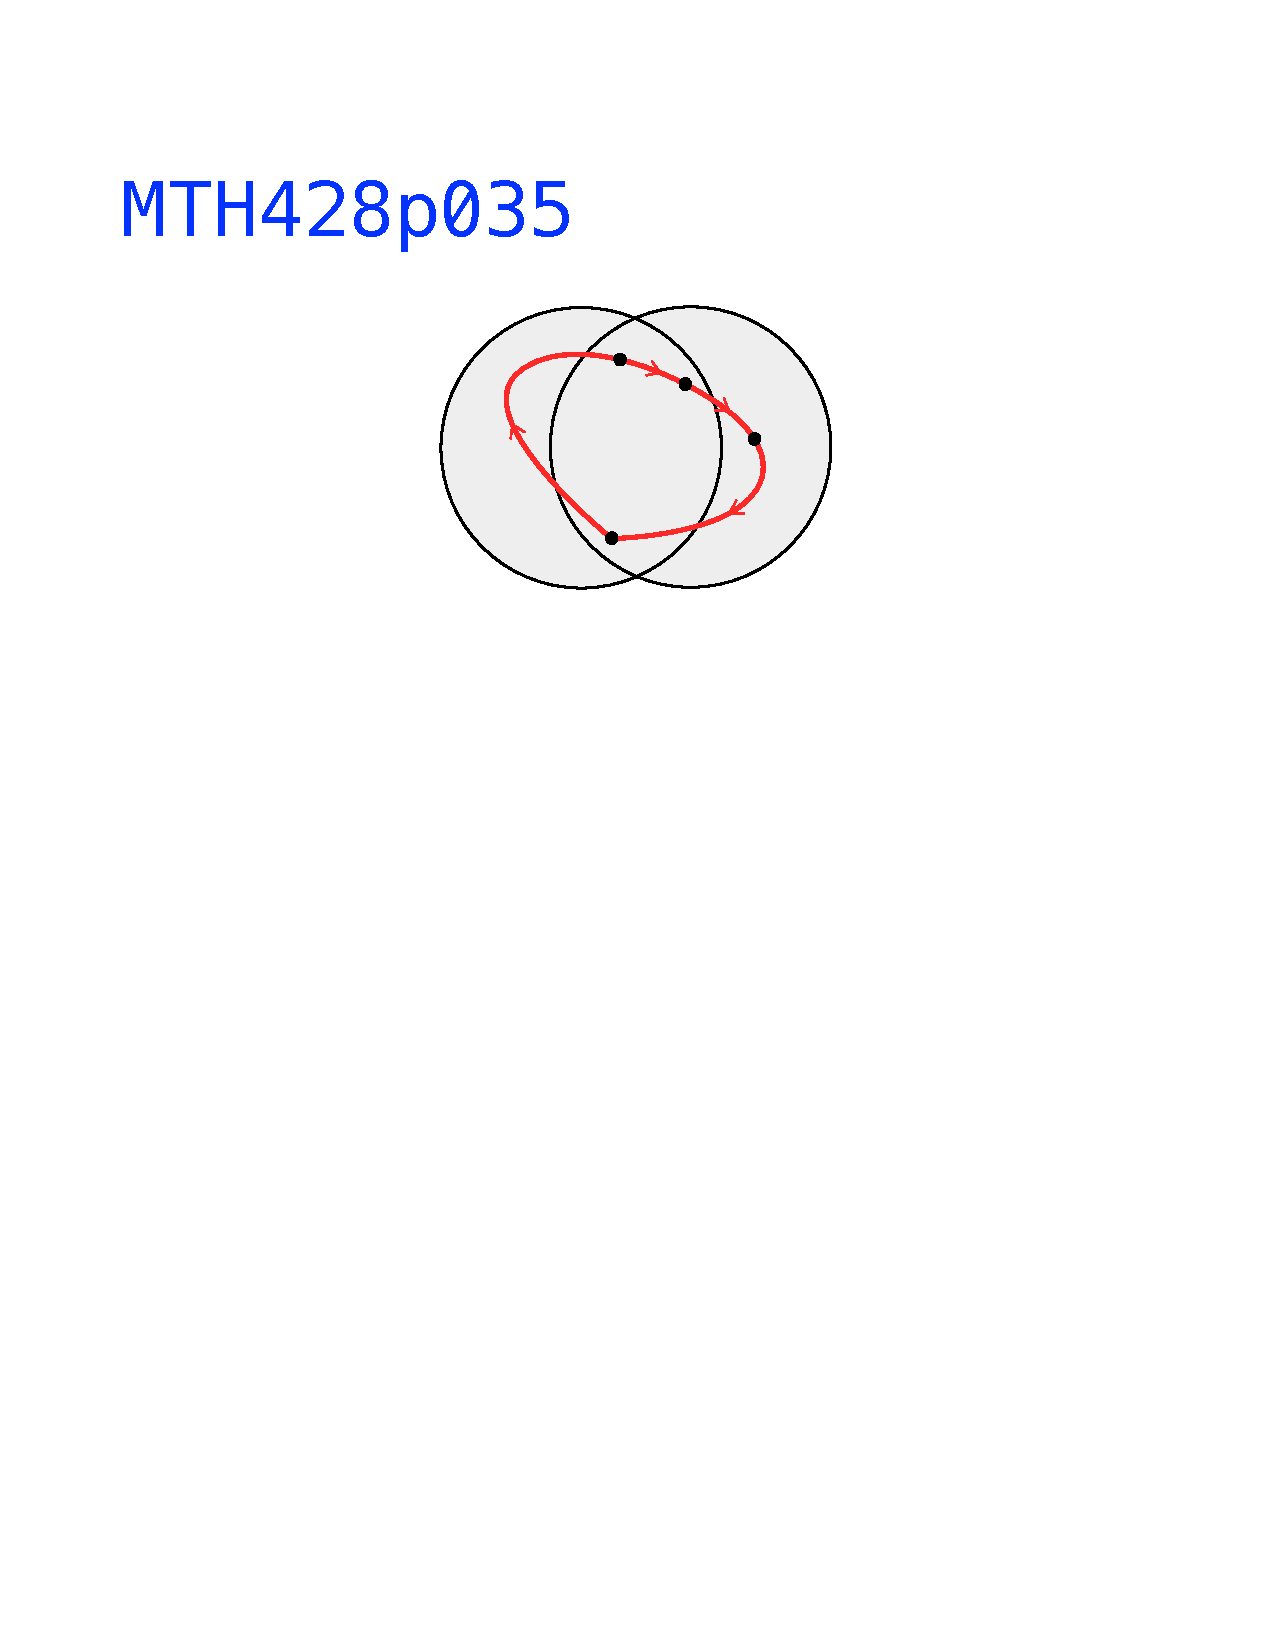
\includegraphics[width=\textwidth, trim=0mm 177mm 0mm 51mm, clip]{pictures/MTH428p035.pdf}}};

%%% COORDINATE GRID
%\draw[step=0.5, help lines] (0,0) to[grid with coordinates] (15,9);
%%% 

\node[anchor= base]  at (8.0 , 1.1){\small  $x_{0}$};
\node[anchor= base]  at (6.0 , 3.4){\small  $U_{1}$};
\node[anchor= base]  at (10.55 , 3.4){\small  $U_{2}$};
\node[anchor= north west]  at (9.55 , 1.29){\color{red} \small  $\omega_{4}$};
\node[anchor= base]  at (9.50 , 2.79){\color{red} \small  $\omega_{3}$};
\node[anchor= base]  at (8.55 , 3.25){\color{red} \small  $\omega_{2}$};
\node[anchor= base]  at (6.39 , 2.14){\color{red} \small  $\omega_{1}$};

\end{tikzpicture}

We have $\omega \simeq   \omega_{1}\ast \omega_{2} \ast \dots \ast \omega_{n}$. 
By the properties of loop completion we get:
$$\omega \simeq \omega^{\circ}\simeq 
\omega_{1}^{\circ}\ast \omega_{2}^{\circ}\ast {\dots} \ast \omega_{n}^{\circ}$$
Moreover, if $\omega_{i}$ is contained in $U_{1}$ then $\omega_{i}^{\circ}$ is a loop in  $U_{1}$, 
and likewise for $U_{2}$. 

\begin{tikzpicture}

\node[anchor=south west,inner sep=0] at (0,0) 
{{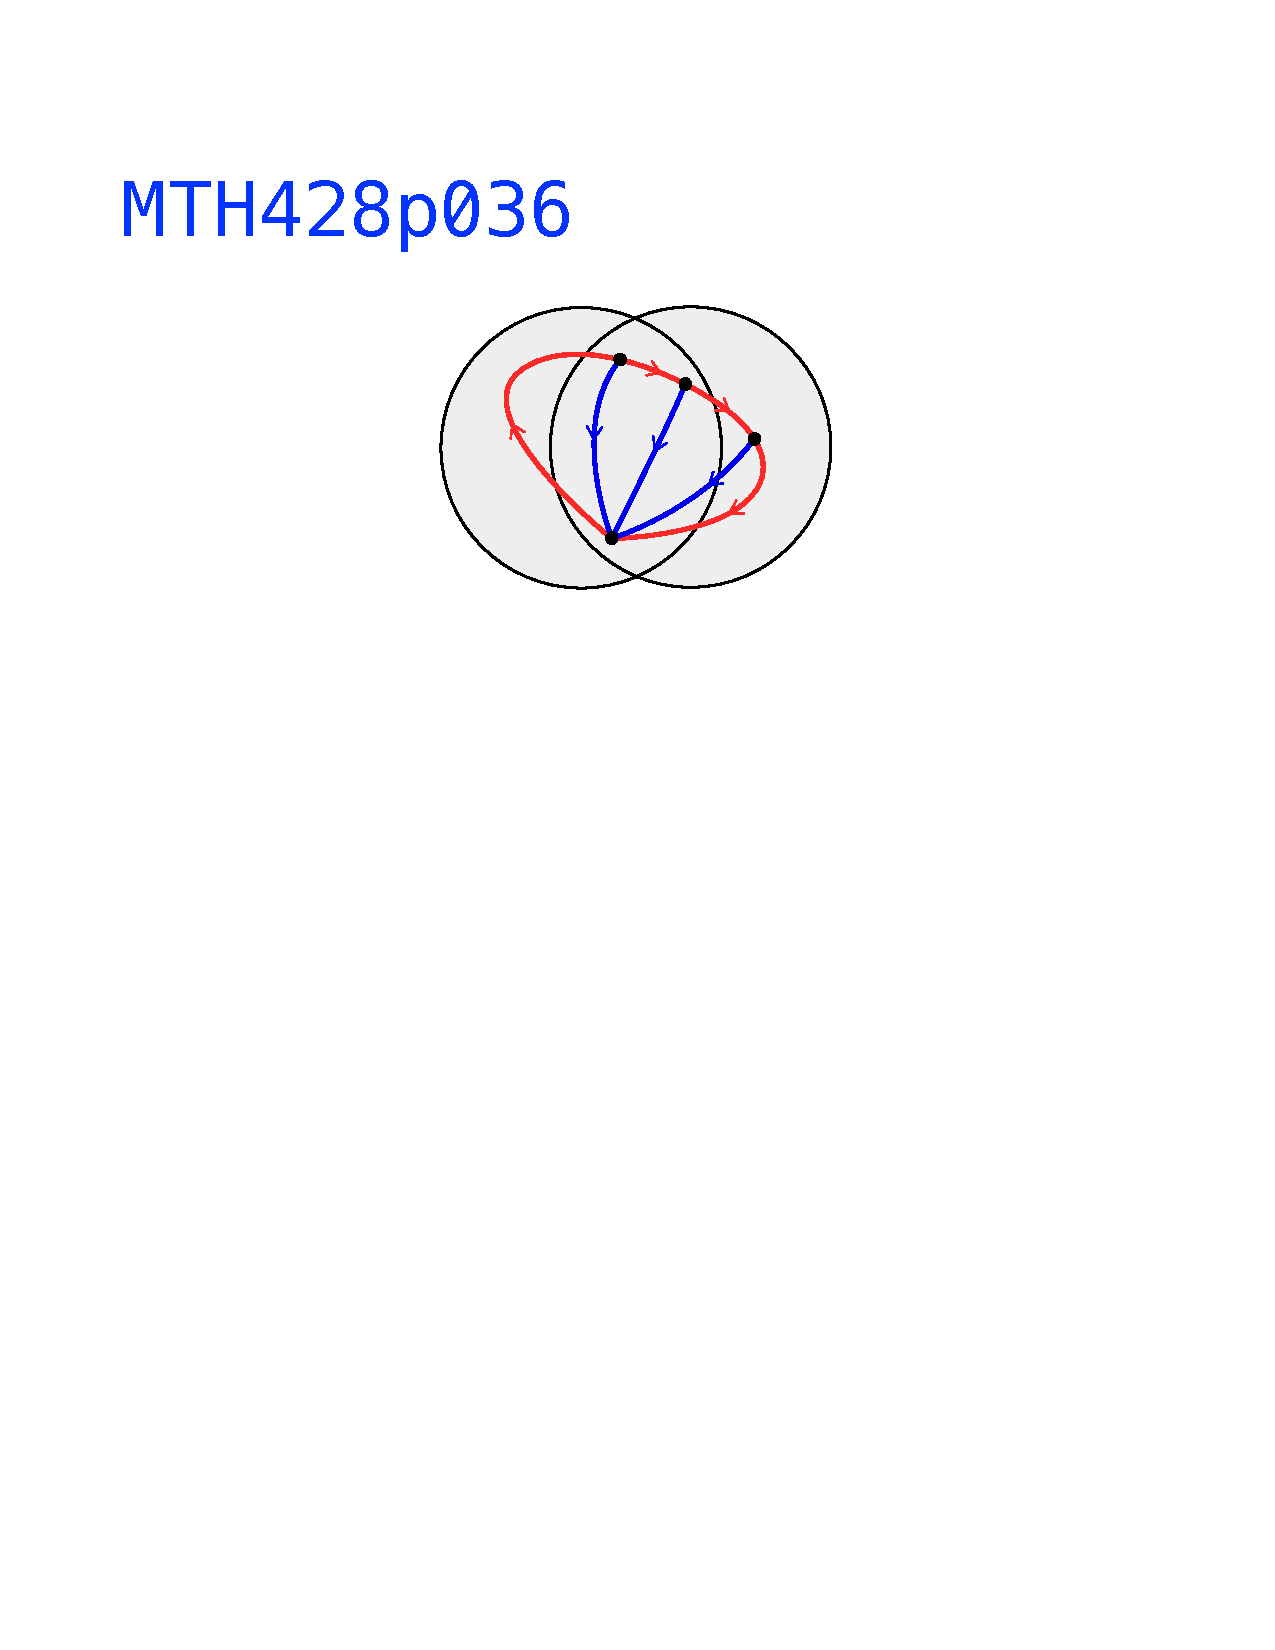
\includegraphics[width=\textwidth, trim=0mm 177mm 0mm 51mm, clip]{pictures/MTH428p036.pdf}}};

%%% COORDINATE GRID
%\draw[step=0.5, help lines] (0,0) to[grid with coordinates] (15,9);
%%% 

\node[anchor= base]  at (6.0 , 3.4){\small  $U_{1}$};
\node[anchor= base]  at (10.55 , 3.4){\small  $U_{2}$};
\node[anchor= north west]  at (9.55 , 1.29){\color{red} \small  $\omega_{4}$};
\node[anchor= base]  at (9.50 , 2.79){\color{red} \small  $\omega_{3}$};
\node[anchor= base]  at (8.55 , 3.25){\color{red} \small  $\omega_{2}$};
\node[anchor= base]  at (6.39 , 2.14){\color{red} \small  $\omega_{1}$};

\end{tikzpicture}

Let $k(i)$ denote either $1$ or $2$ depending if $\omega_{i}^{\circ}$
is a loop in $U_{1}$ or $U_{2}$. Define an element $\ntilde h(\omega)\in G$ by 
\begin{equation*}
\label{VANKH EQ}
\tag{$\ast\ast$}
\ntilde h(\omega) = h_{k(1)}([\omega_{1}^{\circ}]_{k(1)}) \cdot h_{k(2)}([\omega_{2}^{\circ}]_{k(2)})\cdot {\dots}
\cdot  h_{k(n)}([\omega_{n}^{\circ}]_{k(n)})
\end{equation*}
There are two ambiguities in this formula.  First, if $\omega_{i}$ is a path entirely contained 
in $U_{0}$ then $\omega_{i}^{\circ}$ is a loop in $U_{0}$ and in such case we can take $k(i)$
to be either $1$ or $2$. This however does not matter since in such case we have 
$[\omega_{i}]_{1} = i_{1\ast}([\omega_{i}]_{0})$ and $[\omega_{i}]_{2} = i_{2\ast}([\omega_{i}]_{0})$,
and  since $h_{1}i_{1\ast} = h_{2}i_{2\ast}$ we get 
$$h_{1}([\omega_{i}^{\circ}]_{1}) = h_{1}i_{1\ast}([\omega_{i}^{\circ}]_{0}) 
= h_{2}i_{2\ast}([\omega_{i}^{\circ}]_{0}) = h_{2}([\omega_{i}^{\circ}]_{1})$$
The second ambiguity comes from the fact that the formula (\ref{VANKH EQ})  uses 
subdivision of $\omega$ into paths $\omega_{i}$, and the value of $\ntilde{h}(\omega)$ could change 
if we change the subdivision. To see that this is not the case consider the subdivision  
$\omega\simeq \omega_{1}\ast {\dots} \ast \omega_{n}$
that comes from an $n$-tuple of numbers $\underline{s} = (s_{0}, \dots, s_{n})$, and let $s_{+}$ 
be a number such that $s_{i-1} < s_{+} < s_{i}$ for some $1\leq i \leq n$. The $(n+1)$-tuple 
$\underline{s}' = (s_{1}, \dots, s_{i-1}, s_{+}, s_{i+1}, \dots, s_{n})$ produces the subdivision 
$$\omega \simeq \omega_{1}\ast {\dots} \ast \omega_{i-1} \ast \tau_{1}\ast \tau_{2} 
\ast \omega_{i+1} \ast {\dots}\ast \omega_{n}$$
where $\tau_{1}\ast \tau_{2} \simeq \omega_{i}$.  By the properties of loop completion
$[\omega^{\circ}]_{k(i)} = [\tau_{1}^{\circ}]_{k(i)} \cdot [\tau_{2}^{\circ}]_{k(i)}$, and thus we get 
$$h_{k(i)}([\omega_{i}^{\circ}]_{k(i)}) = h_{k(i)}([\tau_{1}^{\circ}]_{k(i)} \cdot [\tau_{2}^{\circ}]_{k(i)})
= h_{k(i)}([\tau_{1}^{\circ}]_{k(i)})\cdot h_{k(i)}([\tau_{2}^{\circ}]_{k(i)})$$
This shows the the value of $\ntilde{h}(\omega)$ does not depend on whether we compute it using  
$\underline{s}$ or $\underline{s}'$. 
Arguing inductively we obtain that if an $m$-tuple $\underline{s}'$ is obtained by 
adding some number of elements to an $n$-tuple $\underline{s}$ then the value of 
$\ntilde{h}(\omega)$ computed using $\underline{s}'$ is the same as the value 
computed using $\underline{s}$. Finally,  given an  arbitrary $n$-tuple 
$\underline{s}$ and an $m$-tuple $\underline{s}'$ that produce two subdivisions 
of $\omega$  we can find an $r$-tuple $\underline{s}''$ that can be obtained from each of  
$\underline{s}$  and $\underline{s}'$ by inserting some additional elements. The argument 
above shows then that the values of $\ntilde{h}(\omega)$ computed using $\underline{s}$
and $\underline{s}'$ must be equal since they are both equal to the value computed using 
$\underline{s}''$.

Our goal will be to show that $\ntilde{h}(\omega)$ depends only on the homotopy class of $\omega$:

\emph{Claim.}  If $\omega$, $\tau$ are loops in $X$ and $\omega\simeq \tau$ 
then $\ntilde{h}(\omega) = \ntilde{h}(\tau)$. 


Assuming for a moment this claim holds notice that it allows us to define a function 
$h\colon \pi_{1}(X, x_{0}) \to G$  by $h([\omega]) = \ntilde{h}(\omega)$. Notice also 
that this function has the following properties: 
\benu
\item[1)] $h$ is a homomorphism;  
\item[2)] $h$ makes the diagram (\ref{VANK PUSHOT EQ}) into a commutative diagram;
\item[3)] $h$ is the only homomorphism that makes the diagram (\ref{VANK PUSHOT EQ}) commute. 
\eenu

Indeed, to see 1) observe that if $\omega$ and $\omega'$ are  two  loops in $X$ with subdivisions 
$\omega \simeq \omega_{1}\ast {\dots}\ast \omega_{n}$ and
$\omega' \simeq \omega'_{1}\ast {\dots}\ast \omega'_{m}$ then $\omega\ast\omega'$ has a subdivision 
$$\omega\ast\omega'\simeq 
 \omega_{1}\ast {\dots}\ast \omega_{n}\ast \omega'_{1}\ast {\dots}\ast \omega'_{m}$$ 
Using this observation and the definition of $h$ we get that 
$h([\omega]\cdot [\omega']) = h([\omega])\cdot h([\omega'])$. 

To verify  2) notice that if $\omega$ is a loop in $U_{k}$  for either $k=1$ or $k=2$ then  we 
don't need to subdivide it, i.e. we can take $\omega = \omega_{1}$. Since 
$\omega \simeq \omega^{\circ}$ the formula (\ref{VANKH EQ}) 
gives 
$$h([\omega]) = \ntilde{h}(\omega) = h_{k}([\omega]_{k})$$
and since  $[\omega] = j_{k\ast}([\omega]_{k})$ we obtain $hj_{k\ast} = h_{k}$. 
 
Finally,  to see 3) notice that we have shown that any element $[\omega]\in \pi_{1}(X, x_{0})$
can be written as a product $[\omega] = [\omega_{1}^{\circ}]\cdot {\dots}\cdot [\omega_{n}^{\circ}]$
where $\omega_{i}$  is a loop in $U_{k(i)}$ for either $k(i)=1$ or $k(i)=2$. For each $i=1, \dots, n$ 
we have $[\omega_{i}^{\circ}] = j_{k(i)\ast}([\omega_{i}^{\circ}]_{k(i)})$. Thus in order to get the identity $hj_{k(i)\ast} = h_{k(i)}$ 
we must set $h([\omega_{i}^{\circ}]) = h_{k(i)}([\omega_{i}^{\circ}]_{k(i)})$. Since homomorphisms preserve products 
we are forced to define $h([\omega])$ by the formula (\ref{VANKH EQ}). 

The above observations show that once we verify that $\ntilde{h}$ is a homotopy 
invariant function the proof of van Kampen's Theorem will be complete. 
Assume then that  $\omega$, $\tau$ are loops in $X$ 
and that there exists a homotopy 
$h\colon [0, 1]\times [0, 1] \to X$ between them: $h_{0} = \omega$, $h_{1}= \tau$. 
We will consider first a special case, and assume 
 in addition that there exists numbers $0= s_{0} < s_{1} < {\dots} < s_{n} = 1$ such that 
the homotopy  $h$ maps each rectangle $[s_{i-1}, s_{i}]\times [0, 1]$ either into $U_{1}$ or
into $U_{2}$.  In particular this gives a subdivisions $\omega\simeq \omega_{1} \ast {\dots} \ast \omega_{n}$
and $\tau \simeq \tau_{1} \ast {\dots} \ast \tau_{n}$ where $\omega_{i}$ and $\tau_{i}$
are restrictions of $\omega$ and $\tau$ to the subinterval $[s_{i-1}, s_{i}]$. For $i=0, \dots, n$
denote by $\gamma_{i}$ the path given by $\gamma(t) = h(s_{i}, t)$. Notice that $\gamma_{0}$ and 
$\gamma_{n}$ are constant paths at $x_{0}$. 

\begin{tikzpicture}

\node[anchor=south west,inner sep=0] at (0,0) 
{{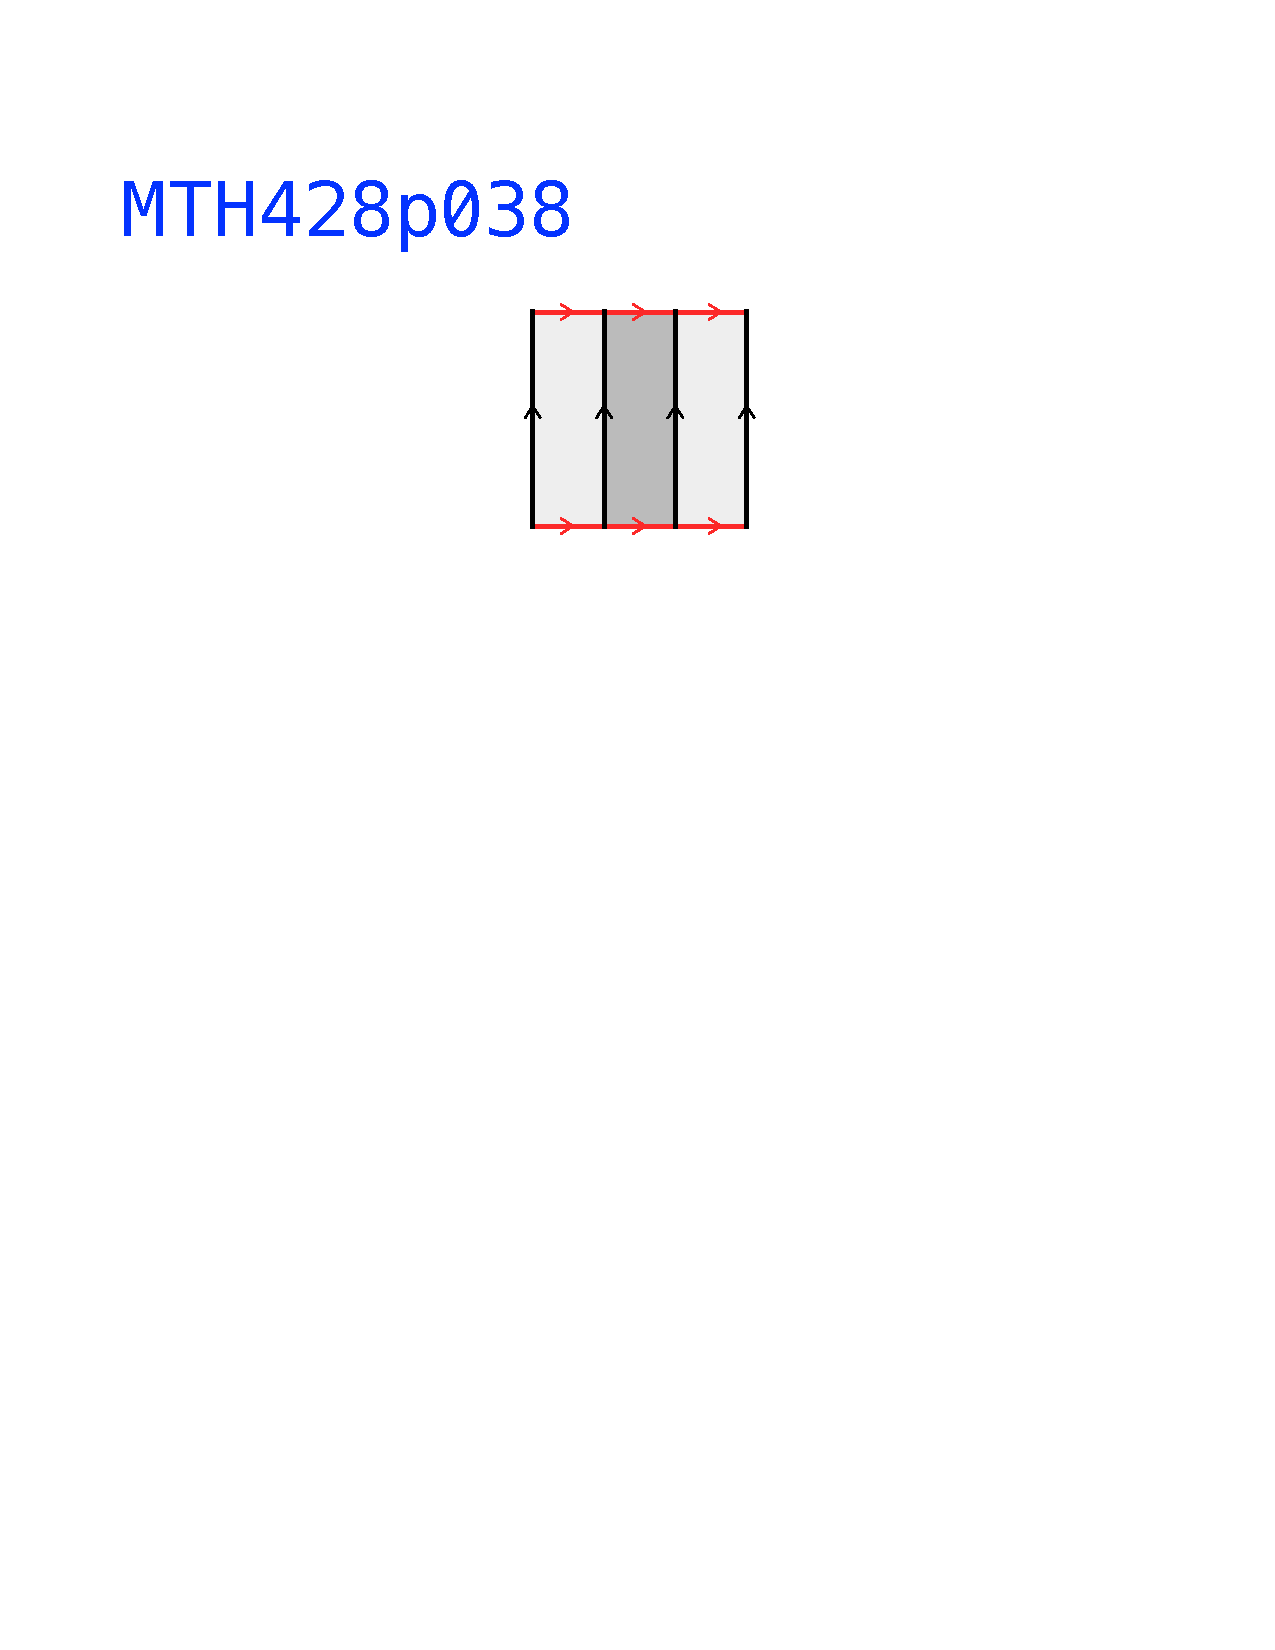
\includegraphics[width=\textwidth, trim=0mm 188mm 0mm 51mm, clip]{pictures/MTH428p038.pdf}}};

%%% COORDINATE GRID
%\draw[step=0.5, help lines] (0,0) to[grid with coordinates] (15,9);
%%% 


\node[anchor= base]  at (7.4 , -0.18){\color{red} \small  $\omega_{1}$};
\node[anchor= base]  at (8.35 , -0.18){\color{red} \small  $\omega_{2}$};
\node[anchor= base]  at (9.3 , -0.18){\color{red} \small  $\omega_{3}$};
\node[anchor= base]  at (7.4 , 3.2){\color{red} \small  $\tau_{1}$};
\node[anchor= base]  at (8.35 , 3.2){\color{red} \small  $\tau_{2}$};
\node[anchor= base]  at (9.3, 3.2){\color{red} \small  $\tau_{3}$};
\node[anchor= base east]  at (6.88, 1.55){ \small  $c_{x_{0}} = \gamma_{0}$};
\node[anchor= base]  at (7.5, 1.55){ \small  $\gamma_{1}$};
\node[anchor= base]  at (9.1, 1.55){ \small  $\gamma_{2}$};
\node[anchor= base west]  at (9.7, 1.55){ \small  $\gamma_{4} = c_{x_{0}}$};
\node[anchor= base]  at (7.4 , 0.5){ \small  $U_{1}$};
\node[anchor= base]  at (8.35 , 0.5){ \small  $U_{2}$};
\node[anchor= base]  at (9.3 , 0.5){ \small  $U_{1}$};


\end{tikzpicture}

Let $k(i)$ denote either $1$ or $2$ depending if $h([s_{i-1}, s_{i}]\times [0, 1])$ is contained in $U_{1}$
or $U_{2}$. Notice that for each $i$ the paths $\omega_{i}$, $\tau_{i}$,  $\gamma_{i-1}$, and $\gamma_{i}$
are paths in $U_{k(i)}$. Moreover, using the restriction of $h$ to $[s_{i-1}, s_{i}]\times [0, 1]$ we obtain 
that the path $\omega_{i}$ is homotopic to $\gamma_{i-1}\ast\tau_{i}\ast\xov{\gamma}_{i}$ 
via a homotopy contained in $U_{k(i)}$. Using the properties of loop completion we obtain
$$[\omega_{i}^{\circ}]_{k(i)} = [(\gamma_{i-1}\ast\tau_{i}\ast\xov{\gamma}_{i})^{\circ}]_{k(i)}
= [\gamma_{i-1}^{\circ}]_{k(i)}\cdot [\tau_{i}^{\circ}]_{k(i)} \cdot [\gamma_{i}^{\circ}]^{-1}_{k(i)}$$
This identity and the formula (\ref{VANKH EQ}) gives:
\begin{align*}
\label{VANKH2 EQ}
\tag{$\ast\ast\ast$}
\ntilde{h}(\omega) 
& = h_{k(1)}([\omega_{1}^{\circ}]_{k(1)}) \cdot h_{k(2)}([\omega_{2}^{\circ}]_{k(2)})\cdot {\dots}
\cdot  h_{k(n)}([\omega_{n}^{\circ}]_{k(n)}) \\
& =  h_{k(1)}[(\gamma_{0}^{\circ}]_{k(1)})
\cdot h_{k(1)}([\tau_{1}^{\circ}]_{k(1)}) 
\cdot h_{k(1)}([\gamma_{1}^{\circ}]_{k(1)})^{-1} \\
&\  \  \cdot  h_{k(2)}[(\gamma_{1}^{\circ}]_{k(2)})
\cdot h_{k(2)}([\tau_{2}^{\circ}]_{k(2)}) 
\cdot h_{k(2)}([\gamma_{1}^{\circ}]_{k(2)})^{-1} \cdot {\dots} \\
&\ \   \cdot   h_{k(n)}[(\gamma_{n-1}^{\circ}]_{k(n)})
\cdot h_{k(n)}([\tau_{n}^{\circ}]_{k(n)}) 
\cdot h_{k(n)}([\gamma_{n}^{\circ}]_{k(n)})^{-1}
\end{align*}
Notice that $h_{k(1)}([\gamma^{\circ}_{1}]_{k(1)})$ and $h_{k(n)}([\gamma^{\circ}_{n}]_{k(n)})$
are trivial elements of $G$ since $\gamma^{\circ}_{1}$ and $\gamma^{\circ}_{n}$ are constant 
loops.  Also,  for  $i=1, \dots n-1$ we have 
$h_{k(i)}([\gamma^{\circ}_{i}]_{k(i)}) = h_{k(i+1)}([\gamma^{\circ}_{i}]_{k(i+1)})$. 
This is obvious if $k(i) = k(i+1)$. If $k(i)\neq k(i+1)$ then this identity still holds since in such case
$\gamma_{i}$ (and thus also $\gamma^{\circ}_{i}$) is contained in $U_{0}$ and then 
$$h_{1}([\gamma_{i}^{\circ}]_{1}) = h_{1}i_{1\ast}([\gamma_{i}^{\circ}]_{0}) 
= h_{2}i_{2\ast}([\gamma_{i}^{\circ}]_{0}) = h_{2}([\gamma_{i}^{\circ}]_{2})$$
Using these observations we can simplify the equation (\ref{VANKH2 EQ}) to 
$$\ntilde{h}(\omega) = 
h_{k(1)}([\tau_{1}^{\circ}]_{k(1)}) \cdot h_{k(2)}([\tau_{2}^{\circ}]_{k(2)})\cdot {\dots}
\cdot  h_{k(n)}([\tau_{n}^{\circ}]_{k(n)})  = \ntilde{h}(\tau)$$

It remains to consider the general case when we are given two  loops $\omega$ and $\tau$ in $X$
such that $\omega\simeq \tau$. Let $h\colon [0, 1]\times [0, 1]\to X$ be a homotopy with 
$h_{0} = \omega$  and $h_{1} = \tau$. The sets $h^{-1}(U_{1})$ and $h^{-1}(U_{2})$ form an 
open cover of $X$. Using the Lebesgue number of this  cover we can find numbers
$0=s_{0} < s_{1} < {\dots} < s_{n} = 1$ and $0=t_{0} < t_{1} < {\dots} < t_{m} = 1$
such that $h$ maps each rectangle $[s_{i-1}, s_{i}]\times [t_{j-1},  t_{j}]$ either into 
$U_{1}$ or into $U_{2}$. Let $\delta_{i}$ be the path given  by $\delta_{i}(s) = h(s, t_{i})$:

\begin{tikzpicture}

\node[anchor=south west,inner sep=0] at (0,0) 
{{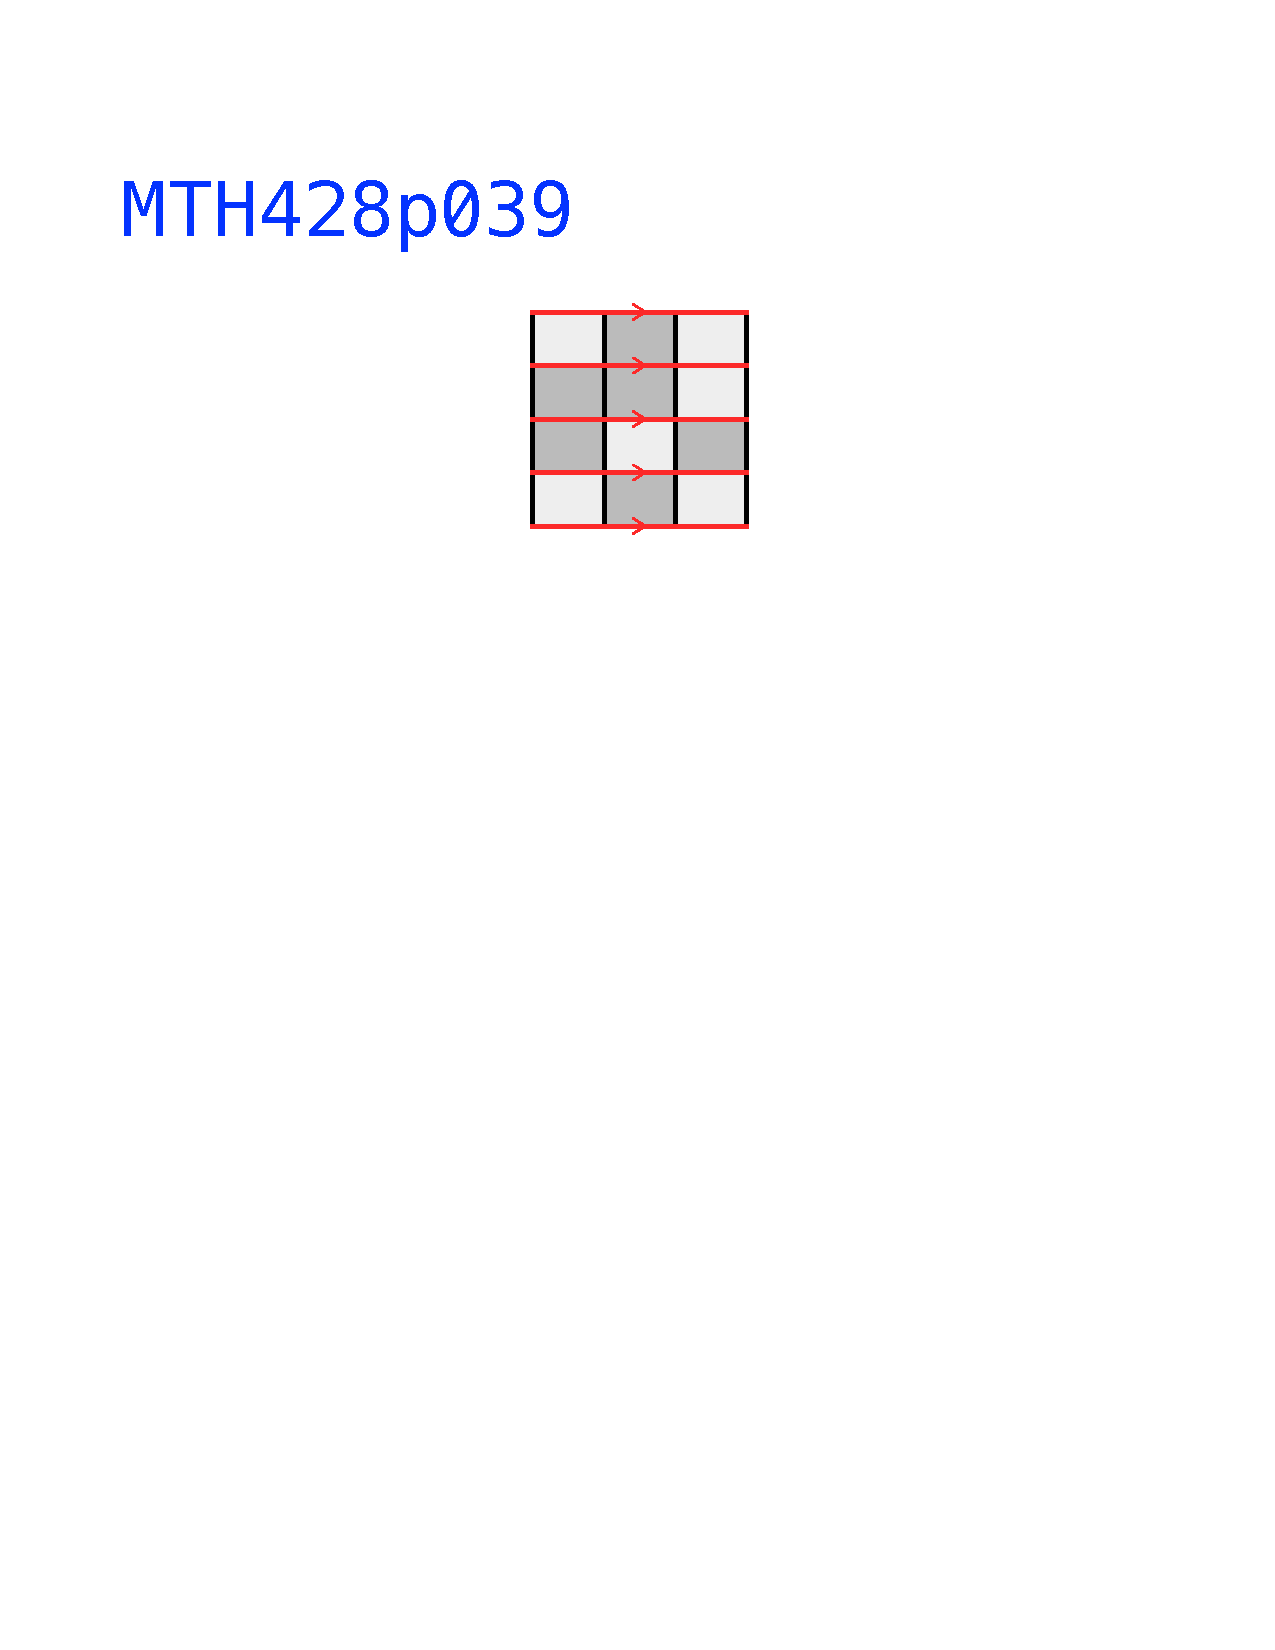
\includegraphics[width=\textwidth, trim=0mm 188mm 0mm 51mm, clip]{pictures/MTH428p039.pdf}}};

%%% COORDINATE GRID
%\draw[step=0.5, help lines] (0,0) to[grid with coordinates] (15,9);
%%% 


\node[anchor=  west]  at (9.75 , 2.98){\color{red} \small  $\delta_{4} = \tau$};
\node[anchor=  west]  at (9.75 , 2.28){\color{red} \small  $\delta_{3}$};
\node[anchor=  west]  at (9.75 , 1.58){\color{red} \small  $\delta_{2}$};
\node[anchor=  west]  at (9.75 , 0.9){\color{red} \small  $\delta_{1}$};
\node[anchor=  west]  at (9.75 , 0.21){\color{red} \small  $\delta_{0} = \omega$};
\node[anchor= base]  at (7.4 , 0.4){ \small  $U_{1}$};
\node[anchor= base]  at (8.35 , 0.4){ \small  $U_{2}$};
\node[anchor= base]  at (9.3 , 0.4){ \small  $U_{1}$};
\node[anchor= base]  at (7.4 , 1.1){ \small  $U_{2}$};
\node[anchor= base]  at (8.35 , 1.1){ \small  $U_{1}$};
\node[anchor= base]  at (9.3 , 1.1){ \small  $U_{2}$};
\node[anchor= base]  at (7.4 , 1.8){ \small  $U_{2}$};
\node[anchor= base]  at (8.35 , 1.8){ \small  $U_{2}$};
\node[anchor= base]  at (9.3 , 1.8){ \small  $U_{1}$};
\node[anchor= base]  at (7.4 , 2.5){ \small  $U_{1}$};
\node[anchor= base]  at (8.35 , 2.5){ \small  $U_{2}$};
\node[anchor= base]  at (9.3 , 2.5){ \small  $U_{1}$};




\end{tikzpicture}

Notice that the restriction of $h$ to the rectangle $[0, 1]\times [t_{i-1}, t_{i}]$ gives a homotopy between 
$\delta_{i-1}$ and $\delta_{i}$, and moreover this homotopy is of the form considered in the special 
case above. Therefore for each $i=1, \dots, m$ we have $\ntilde{h}(\delta_{i-1}) = \ntilde{h}(\delta_{i})$.
As a consequence we obtain 
$$\ntilde{h}(\omega) = \ntilde{h}(\delta_{0}) = \ntilde{h}(\delta_{1}) = {\dots} = \ntilde{h}(\delta_{m}) = 
\ntilde{h}(\tau)$$

\end{proof}


Theorem \ref{VANKAMPEN THM} can be generalized to the case where the space $X$ 
is covered by more that two (and possibly inifinitely many) open sets:


%---BBLANK 
\begin{theorem}
\label{GENVANK THM}
Let $(X, x_{0})$ be a pointed topological space and let $\{U_{i}\}_{i\in I}$ be an open cover of $X$ such that 
$x_{0}\in U_{i}$ for all $i\in I$. For $i, j\in I$ let $f_{ij}\colon U_{i}\cap U_{j} \to U_{i}$ denote the inclusion
map.  If the set $U_{i} \cap U_{j} \cap U_{k}$ is path connected 
for all $i, j, k\in I$ then 
$$\pi_{1}(X, x_{0}) \cong \ast_{i\in I} \pi_{1}(U_{i}, x_{0})/N$$
where $N$ is the normal subgroup of $\ast_{i\in I} \pi_{1}(U_{i}, x_{0})$ generated by all elements 
of the form $f_{ij}([\omega])\cdot f_{ji}([\omega])^{-1}$ for $i, j\in I$ and 
$[\omega]\in \pi_{1}(U_{i}\cap U_{j}, x_{0})$.
\end{theorem}
%---EBLANK  # \newpage

Here is one application of the generalized  van Kampen Theorem:


%---BBLANK 
\begin{proposition}
\label{PI1WEDGE PROP}
Let $\{(X_{i}, x_{i})\}_{i\in I}$ be a family of path connected pointed spaces, and let $\bigvee_{i\in I} X_{i}$ be the 
space obtained by identifying the basepoints $x_{i}\sim x_{j}$ for all $i, j\in I$. Assume that for each $i\in I$
there exists a set $V_{i}\subseteq X_{i}$ such that $V_{i}$ is open in $X_{i}$, $x_{i}\in V_{i}$, and 
the one-point space $\{x_{i}\}$ is a deformation retract of $V_{i}$.  Then  
$$\pi_{1}(\textstyle{\bigvee_{i}} X_{i}) \cong \ast_{i\in I}\pi_{1}(X_{i}, x_{i})$$


\begin{equation*}
\begin{tikzpicture}[
    scale = 1.7,
    d0/.style = {thick, fill=mygray1}
]


\fill[mygray1, scale=0.3, , rotate around= {90:(0,0)}, xshift=2pt]
(0,0) .. controls +(0,0) and +(-1,0) .. 
(2.5, 1.2) .. controls +(0.5,0) and +(0, 0.7).. 
(3.5,0)  ..controls +(0, -0.7) and +(0.5, 0)..  
(2.5,-1.2) ..controls +(-1, 0) and +(0,0).. 
cycle;

\fill[mygray1, scale=0.3, rotate around= {-90:(0,0)}, xshift=2pt]
(0,0) .. controls +(0,0) and +(-1,0) .. 
(2.5, 1.2) .. controls +(0.5,0) and +(0, 0.7).. 
(3.5,0)  ..controls +(0, -0.7) and +(0.5, 0)..  
(2.5,-1.2) ..controls +(-1, 0) and +(0,0).. 
cycle;

\fill[mygray1,scale=0.3,, rotate around= {180:(0,0)}, xshift=2pt]
(0,0) .. controls +(0,0) and +(-1,0) .. 
(2.5, 1.2) .. controls +(0.5,0) and +(0, 0.7).. 
(3.5,0)  ..controls +(0, -0.7) and +(0.5, 0)..  
(2.5,-1.2) ..controls +(-1, 0) and +(0,0).. 
cycle;

\begin{scope}
\clip[scale=0.3, rotate around= {90:(0,0)}, xshift=2pt]
(0,0) .. controls +(0,0) and +(-1,0) .. 
(2.5, 1.2) .. controls +(0.5,0) and +(0, 0.7).. 
(3.5,0)  ..controls +(0, -0.7) and +(0.5, 0)..  
(2.5,-1.2) ..controls +(-1, 0) and +(0,0).. 
cycle;
\fill[mypink] (0,0) circle (0.62);
\end{scope}


\begin{scope}
\clip[scale=0.3, rotate around= {-90:(0,0)}, xshift=2pt]
(0,0) .. controls +(0,0) and +(-1,0) .. 
(2.5, 1.2) .. controls +(0.5,0) and +(0, 0.7).. 
(3.5,0)  ..controls +(0, -0.7) and +(0.5, 0)..  
(2.5,-1.2) ..controls +(-1, 0) and +(0,0).. 
cycle;
\fill[mypink] (0,0) circle (0.62);
\end{scope}

\begin{scope}
\clip[scale=0.3, rotate around= {180:(0,0)}, xshift=2pt]
(0,0) .. controls +(0,0) and +(-1,0) .. 
(2.5, 1.2) .. controls +(0.5,0) and +(0, 0.7).. 
(3.5,0)  ..controls +(0, -0.7) and +(0.5, 0)..  
(2.5,-1.2) ..controls +(-1, 0) and +(0,0).. 
cycle;
\fill[mypink] (0,0) circle (0.62); 
\end{scope}

\draw[scale=0.3,  thick, rotate around= {90:(0,0)}, xshift=2pt]
(0,0) .. controls +(0,0) and +(-1,0) .. 
(2.5, 1.2) .. controls +(0.5,0) and +(0, 0.7).. 
(3.5,0)  ..controls +(0, -0.7) and +(0.5, 0)..  
(2.5,-1.2) ..controls +(-1, 0) and +(0,0).. 
cycle;

\draw[scale=0.3,  thick, rotate around= {-90:(0,0)}, xshift=2pt]
(0,0) .. controls +(0,0) and +(-1,0) .. 
(2.5, 1.2) .. controls +(0.5,0) and +(0, 0.7).. 
(3.5,0)  ..controls +(0, -0.7) and +(0.5, 0)..  
(2.5,-1.2) ..controls +(-1, 0) and +(0,0).. 
cycle;

\draw[scale=0.3,  thick, rotate around= {180:(0,0)}, xshift=2pt]
(0,0) .. controls +(0,0) and +(-1,0) .. 
(2.5, 1.2) .. controls +(0.5,0) and +(0, 0.7).. 
(3.5,0)  ..controls +(0, -0.7) and +(0.5, 0)..  
(2.5,-1.2) ..controls +(-1, 0) and +(0,0).. 
cycle;

\draw[line width = 1.6, dotted] ({(0.65*cos(-51)}, {0.65*sin(-51)}) arc (-51:51:0.65);
\filldraw (0,0) circle (0.05);


\node[red] at (0.01, 0.37) {\small $V_{i_{1}}$}; 
\node at (0.02, 0.8) {\small $X_{i_{1}}$}; 
\node[red] at (0.01, -0.37) {\small $V_{i_{3}}$}; 
\node at (0.03, -0.8) {\small $X_{i_{3}}$}; 
\node[red] at (-0.37, 0) {\small $V_{i_{2}}$}; 
\node at (-0.8, 0) {\small $X_{i_{2}}$}; 

\end{tikzpicture}
\end{equation*}


\end{proposition}
%---EBLANK  # \newpage


\begin{proof}
We will denote by $\xov{x}$ the point of $\bigvee_{i\in I} X_{i}$ obtained by identifying the points 
$x_{i}\in X_{i}$. 
For $i\in I$ let $U_{i} = X_{i} \vee \bigvee_{i\in} V_{i}$. The sets $U_{i}$ are path connected 
and the form an open cover $\bigvee_{i} X_{i}$. Moreover for $j, k. l \in I$ we have
$$
U_{j}\cap U_{k} \cap U_{l} = 
\begin{cases}
U_{j} & \text{ if } j=k=l \\
\bigvee_{i\in I} V_{i} & \text{ otherwise}
\end{cases}
$$ 
so $U_{j}\cap U_{k} \cap U_{l}$ is path connected for all $j, k, l$. Using Theorem \ref{GENVANK THM}
we obtain
$$\pi_{1}(\textstyle{\bigvee_{i\in I}} X_{i}, \xov{x}) \cong \ast_{i\in I} \pi_{1}(U_{i}, x_{i})/N$$
where $N$ is the normal group generated by elements $f_{ij\ast}([\omega])\cdot f_{ji\ast}([\omega])^{-1}$
for $[\omega]\in \pi_{1}(U_{i}\cap U_{j}, \xov{x})$. As in Theorem \ref{GENVANK THM} by $f_{ij}$
we denote here the inclusion map $f_{ij}\colon U_{i}\cap U_{j}\to U_{ij}$. 
For $i\in I$ let $h_{i}\colon V_{i}\times [0, 1] \to V_{i}$ the deformation retraction of $V_{i}$ onto $\{x_{i}\}$. 
These maps define a deformation retraction of the space $\bigvee_{i\in I} V_{i}$ onto $\{\xov{x}\}$. 
This shows that the space $\bigvee_{i\in I} V_{i}$ is contractible and so 
$\pi_{1}(\bigvee_{i\in I} V_{i}, \xov{x}) = \{1\}$.  
Since for all $i, j\in I$ such that $i\neq j$ we have $U_{i}\cap U_{j} = \bigvee_{i\in I} V_{i}$ it follows that 
the group $N$ is trivial and so 
$\pi_{1}(\textstyle{\bigvee_{i\in I}} X_{i}, \xov{x}) \cong \ast_{i\in I} \pi_{1}(U_{i}, x_{i})$. Finally, 
using again the deformation retractions $h_{i}$ we can construct for each $j\in I$ a deformations retraction 
of $U_{j}$ onto $X_{j}$. This shows that $\pi_{1}(U_{j}, \xov{x})\cong \pi_{1}(X_{j}, \xov{x})$, and so we get 
$$\pi_{1}({\textstyle \bigvee_{i\in I}} X_{i}, \xov{x}) \cong \ast_{i\in I} \pi_{1}(U_{i}, \xov{x}) 
\cong \ast_{i\in I} \pi_{1}(X_{i}, \xov{x})$$
\end{proof}


\begin{example}
Let $s_{0}$ be a basepoint of $S^{1}$. Taking $V = S^{1}\ssmin \{s_{1}\}$ were $s_{1}\in S^{1}$ is a point 
different from $s_{0}$ we obtain an open neighborhood of $s_{0}$ which deformation retracts 
onto $\{x_{0}\}$. Thus using Proposition \ref{PI1WEDGE PROP} we get
$$\pi_{1}(\textstyle{\bigvee_{i\in I}} S^{1}) \cong \ast_{i\in I} \pi_{1}(S^{1})\cong \ast_{i\in I} \Z$$
\end{example}


%%%%%%%%%%%%%%%%%%%%%%%%%%%%%%%
%  EXERCISES
%%%%%%%%%%%%%%%%%%%%%%%%%%%%%%%

\exercises






\newpage
%%%%%%%%%%%%%%%%%%%%%%%%%%%%%%%
%%%%%%%%%%%%%%%%%%%%%%%%%%%%%%%
%%%
%%%  CW COMPLEXES
%%%
%%%%%%%%%%%%%%%%%%%%%%%%%%%%%%%
%%%%%%%%%%%%%%%%%%%%%%%%%%%%%%%

%---BBLANK  
\chapter[CW Complexes]{CW Complexes}
%---EBLANK  
\chaptermark{CW Complexes}

\thispagestyle{firststyle}

Van Kampen's theorem tells us that in order to compute the fundamental group 
of a complicated space we may try to decompose the space into simpler pieces. Information 
about these pieces and how they fit together suffices to determine the fundamental group
of the whole space. A similar approach works in many settings, and for this reason 
it is useful if we can represent a given space as a collection of some simple building blocks 
that are assembled together. In this chapter we discuss the notion of a CW-complex that provides 
a scheme for constructing such representations of spaces. In this scheme as the building blocks
one uses  closed discs of various dimensions. We will see that many interesting spaces can be given 
the structure of a CW-complex. In the next chapters we will see how to compute the fundamental 
group of an arbitrary CW-complex. Building on this result we will  also show that any 
group can be realized as the fundamental group of some space: given a group $G$ we will 
construct a CW-complex $X$ such that $\pi_{1}(X)\cong G$. 


%---BBLANK  
\begin{definition}
Let $X$ be a space and let $f\colon S^{n-1} \to X$ be a continuous function. 
We say that a space $Y$ is obtained by \emph{attaching an $n$-cell}
to $X$ if $Y = X \sqcup D^{n}/{\sim}$
where $\sim$ is the equivalence relation given by $x\sim f(x)$ for all $x\in S^{n-1}\subseteq D^{n}$. 
We write $Y = X \cup_{f} e^{n}$. 

\begin{tikzpicture}
\node[anchor=south west,inner sep=0] at (0,0) 
{{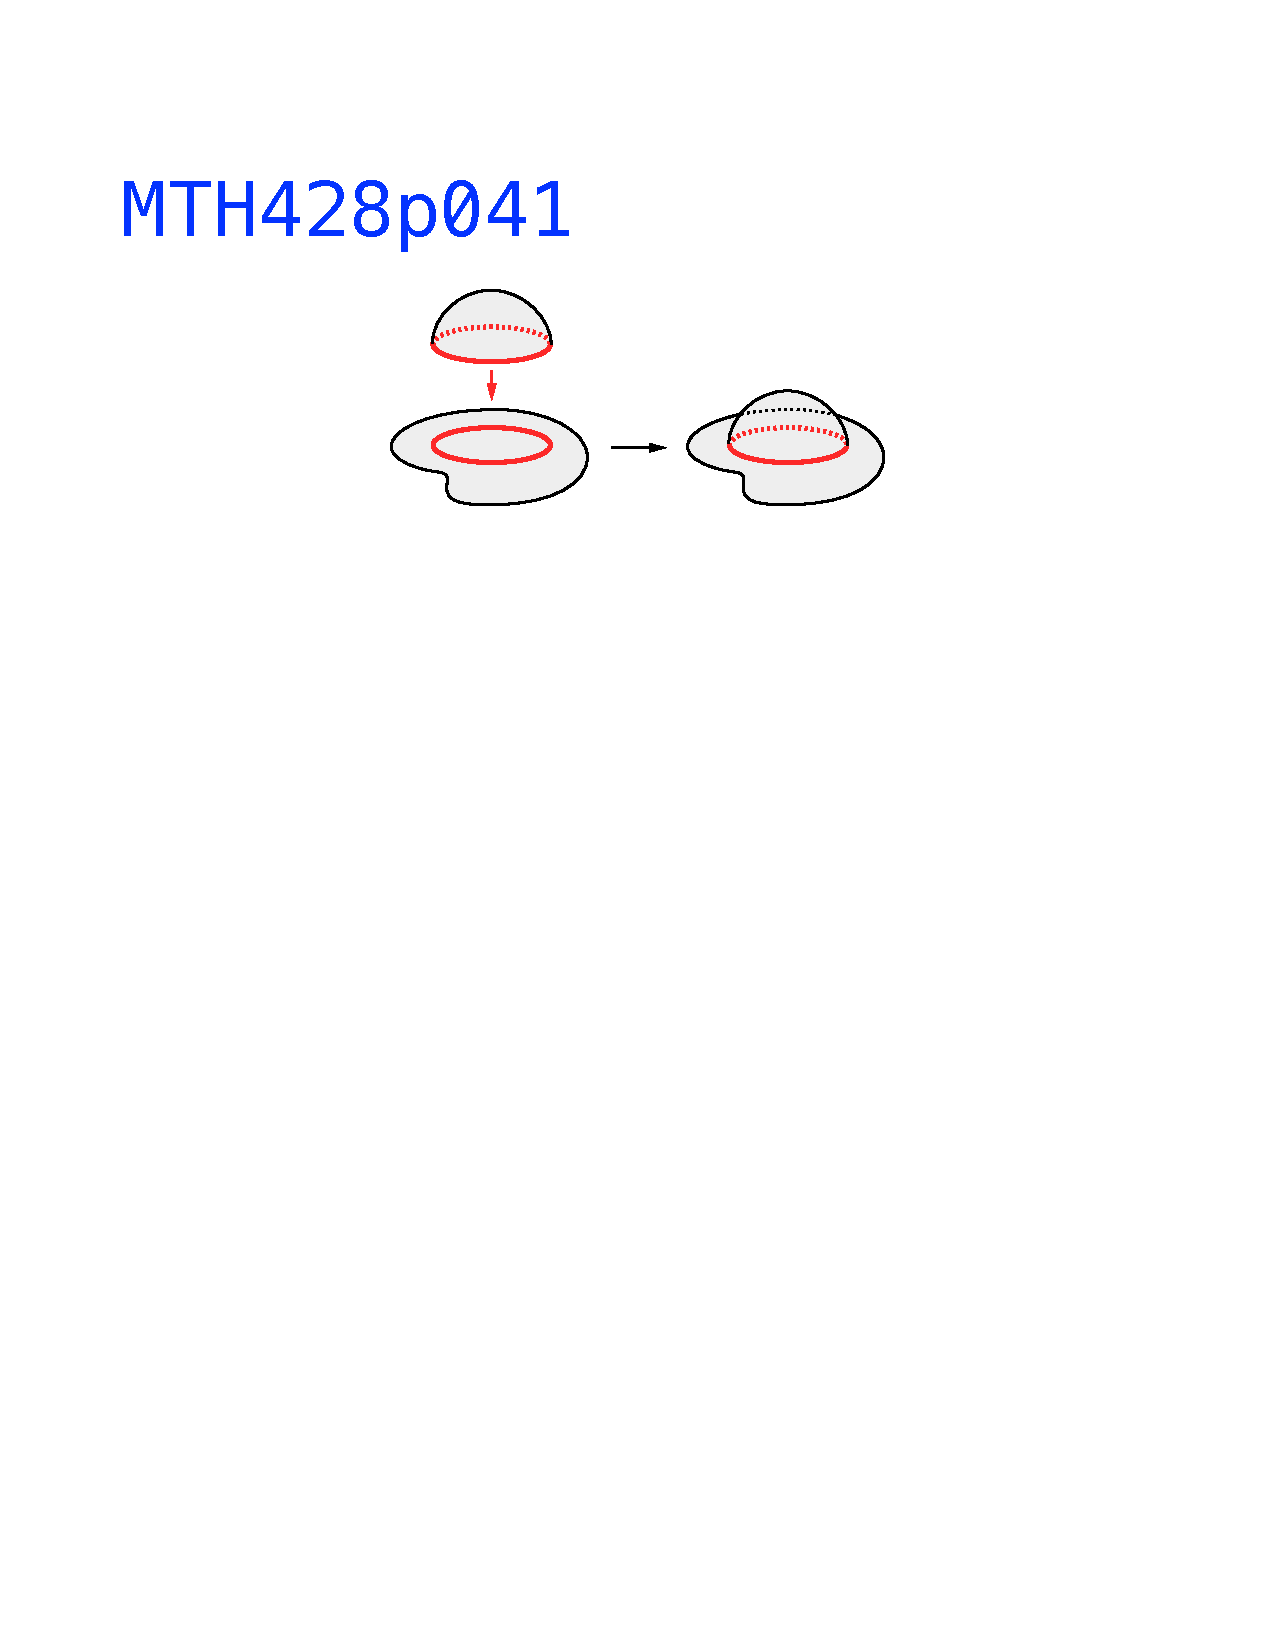
\includegraphics[width=\textwidth, trim=0mm 192mm 0mm 48mm, clip]{pictures/MTH428p041.pdf}}};

%%% COORDINATE GRID
%\draw[step=0.5, help lines] (0,0) to[grid with coordinates] (15,9);
%%% 

\node[anchor=  base]  at (6.7 , 1.6){\color{red} \small  $f$};
\end{tikzpicture}

\end{definition}
%---EBLANK  # \vskip 40mm


Notice that $X\cup_{f} e^{n} = \colim(D^{n} \overset{j}{\la} S^{n-1} \overset{f}{\to} X)$ where 
$j\colon S^{n-1} \to D^{n}$ is the inclusion map.  


%---BBLANK  #
\begin{nn}
%---EBLANK  #  {\bf Some terminology.}
%---BBLANK  #
Here is some terminology associated to the operation of cell attachment:

\benu
\item[\textbullet] The map $f\colon S^{n-1} \to X$ is called the \emph{attaching map} of the cell $e^{n}$. 
\item[\textbullet]  The map $\bar{f} \colon D^{n} \to X \sqcup D^{n} \to X\cup_{f} e^{n}$ is called 
the \emph{characteristic map} of the cell $e^{n}$. 
\item[\textbullet] The subspace $e^{n} = \bar{f}(D^{n}\ssmin S^{n-1}) \subseteq X\cup_{f}e^{n}$ is called 
the \emph{open cell}. 
\item[\textbullet] The subspace $\xov{e}^{n} = \bar{f}(D^{n}) \subseteq X\cup_{f}e^{n}$ is called 
the \emph{closed cell}. 
\eenu
\end{nn}
%---EBLANK # \newpage

\begin{example}
For $n=0$ we have $D^{0} = \{\ast\}$ and $S^{-1} = \varnothing$. Therefore $X\cup e^{0}$ is a disjoint 
union of $X$ and a point.  
\end{example}

\begin{example}
For $n=1$ we have $D^{1} = [-1, 1]$ and $S^{0}= \{-1, 1\}$. The space $X\cup_{f} e^{1}$ is obtained 
by attaching to $X$ an arch or a loop, depending if $f\colon S^{0} \to X$ is a 1-1 function or not:
 
 \begin{tikzpicture}

\node[anchor=south west,inner sep=0] at (0,0) 
{{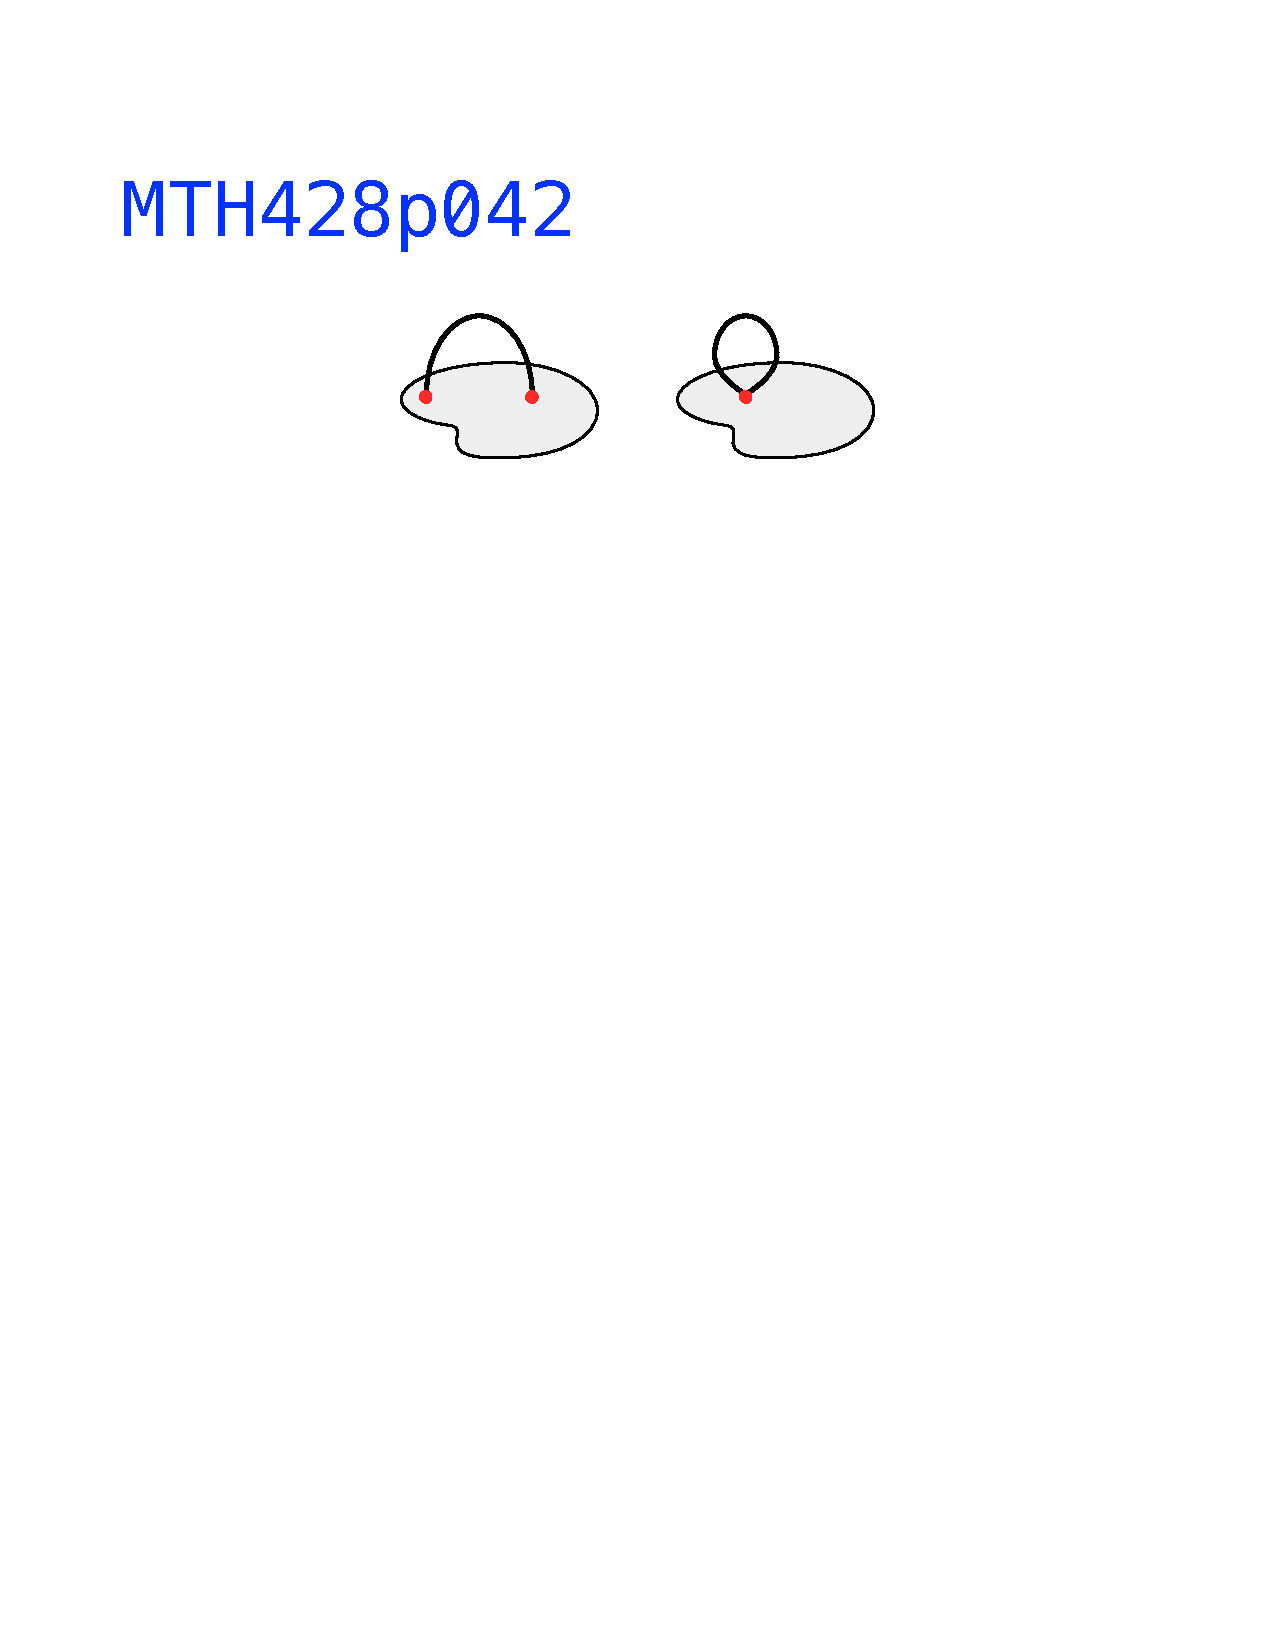
\includegraphics[width=\textwidth, trim=0mm 199mm 0mm 49mm, clip]{pictures/MTH428p042.pdf}}};

%%% COORDINATE GRID
%\draw[step=0.5, help lines] (0,0) to[grid with coordinates] (15,9);
%%% 


\node[anchor=  base]  at (6.1 , 0.87){\color{red} \small  $f(-1)$};
\node[anchor=  base]  at (7.32 , 0.87){\color{red} \small  $f(1)$};
\node[anchor=  base west]  at (9.7 , 0.87){\color{red} \small  $f(\pm1)$};
\node[anchor=  base]  at (6.3 , 2.2){ \small  $e^{1}$};
\node[anchor=  base]  at (9.75 , 2.2){ \small  $e^{1}$};
\end{tikzpicture}
 
\end{example}

In general, the operation of cell attachment can be viewed as a special case of the construction of 
a mapping cone:


%---BBLANK #\  \vskip 150mm
\begin{lemma}
\label{CONEEQCELL LEMMA}
For any map $f\colon S^{n-1}\to X$ the space $X\cup_{f} e^{n}$ is homeomorphic to 
the mapping cone $C_{f}$. 
\end{lemma}

\begin{proof}
Exercise. 
\end{proof}
%---EBLANK # \vskip 20mm

This immediately gives the following fact:

%---BBLANK
\begin{proposition}
\label{CELLSLIDE PROP}
If $f, g\colon S^{n-1}\to X$ are maps such that $f\simeq g$ then $X\cup_{f} e^{n} \simeq X\cup_{g} e^{n}$. 
\end{proposition}
%---EBLANK # \newpage





\begin{proof}[Proof of Proposition \ref{CELLSLIDE PROP}]
Follows from Lemma \ref{CONEEQCELL LEMMA} and Proposition \ref{CONESLIDE PROP}.
\end{proof}



%---BBLANK
\begin{definition}
\label{RELCW DEF}
Let $X$ be topological space and let $Y\subseteq X$. The pair $(X, Y)$ is 
a \emph{relative CW-complex} (or a \emph{relative cell complex}) if $X = \bigcup_{n=-1}^{\infty} X^{(n)}$
where 
\benu
\item[1)]
$X^{(-1)} = Y$;
\item[2)] for $n\geq 0$ the space $X^{(n)}$ is obtained by attaching $n$-cells to $X^{(n-1)}$;
\item[3)] the topology on $X$ is defined so that a set $U\subseteq X$ is open if and only if
$U\cap X^{(n)}$ is open in $X^{(n)}$ for all $n$. 
\eenu
\end{definition}
%---EBLANK 

%---BBLANK # \vskip 60mm
\begin{note}
By part 3) of Definition \ref{RELCW DEF} if $(X, Y)$ is a relative CW-complex then a function 
$f\colon X\to Z$ is continuous if and only if $f|_{X^{(n)}}\colon X^{(n)} \to Z$ is continuous for all $n\geq -1$. 
\end{note}
%---EBLANK 


%---BBLANK # \vskip 40mm
\begin{note}
If $(X, Y)$ is a relative CW-complex then the space $X^{(n)}$ is called \emph{the $n$-skeleton}
of $X$. 
\end{note}
%---EBLANK 

%---BBLANK # \vskip 20mm
\begin{definition}
A \emph{CW-complex} (or a \emph{cell complex}) is a space $X$ such that $(X, \varnothing)$
is a relative CW-complex.  
\end{definition}
%---EBLANK # \newpage

%---BBLANK
\begin{definition}
1) A CW-complex $X$ is \emph{finite} if it consists of finitely many cells. 

2) A CW-complex $X$ is \emph{finite dimensional} if $X= X^{(n)}$ for some $n$. 

3) The \emph{dimension} of a CW-complex $X$ is defined by 
$$
\dim X =
\begin{cases}
\min\{n \ | \  X = X^{(n)} \} & \text{ if $X$ is finite dimensional} \\
\infty  & \text{otherwise}
\end{cases}
$$
\end{definition}
%---EBLANK # \newpage

\begin{example} The only CW-complex of dimension $-1$ is the empty space. A CW-complex of 
dimension $0$ is a discrete topological space (with each point defining a $0$-cell). 


\begin{example}
If a space can be equipped with a structure of a CW-complex of dimension greater than $0$ then such 
structure is not unique. Here  are two different CW-complex structures on $S^{1}$, one  with two $0$-cells and 
two $1$-cells, and  the other with one $0$-cell and one $1$-cell:
\end{example}

\begin{tikzpicture}

\node[anchor=south west,inner sep=0] at (0,0) 
{{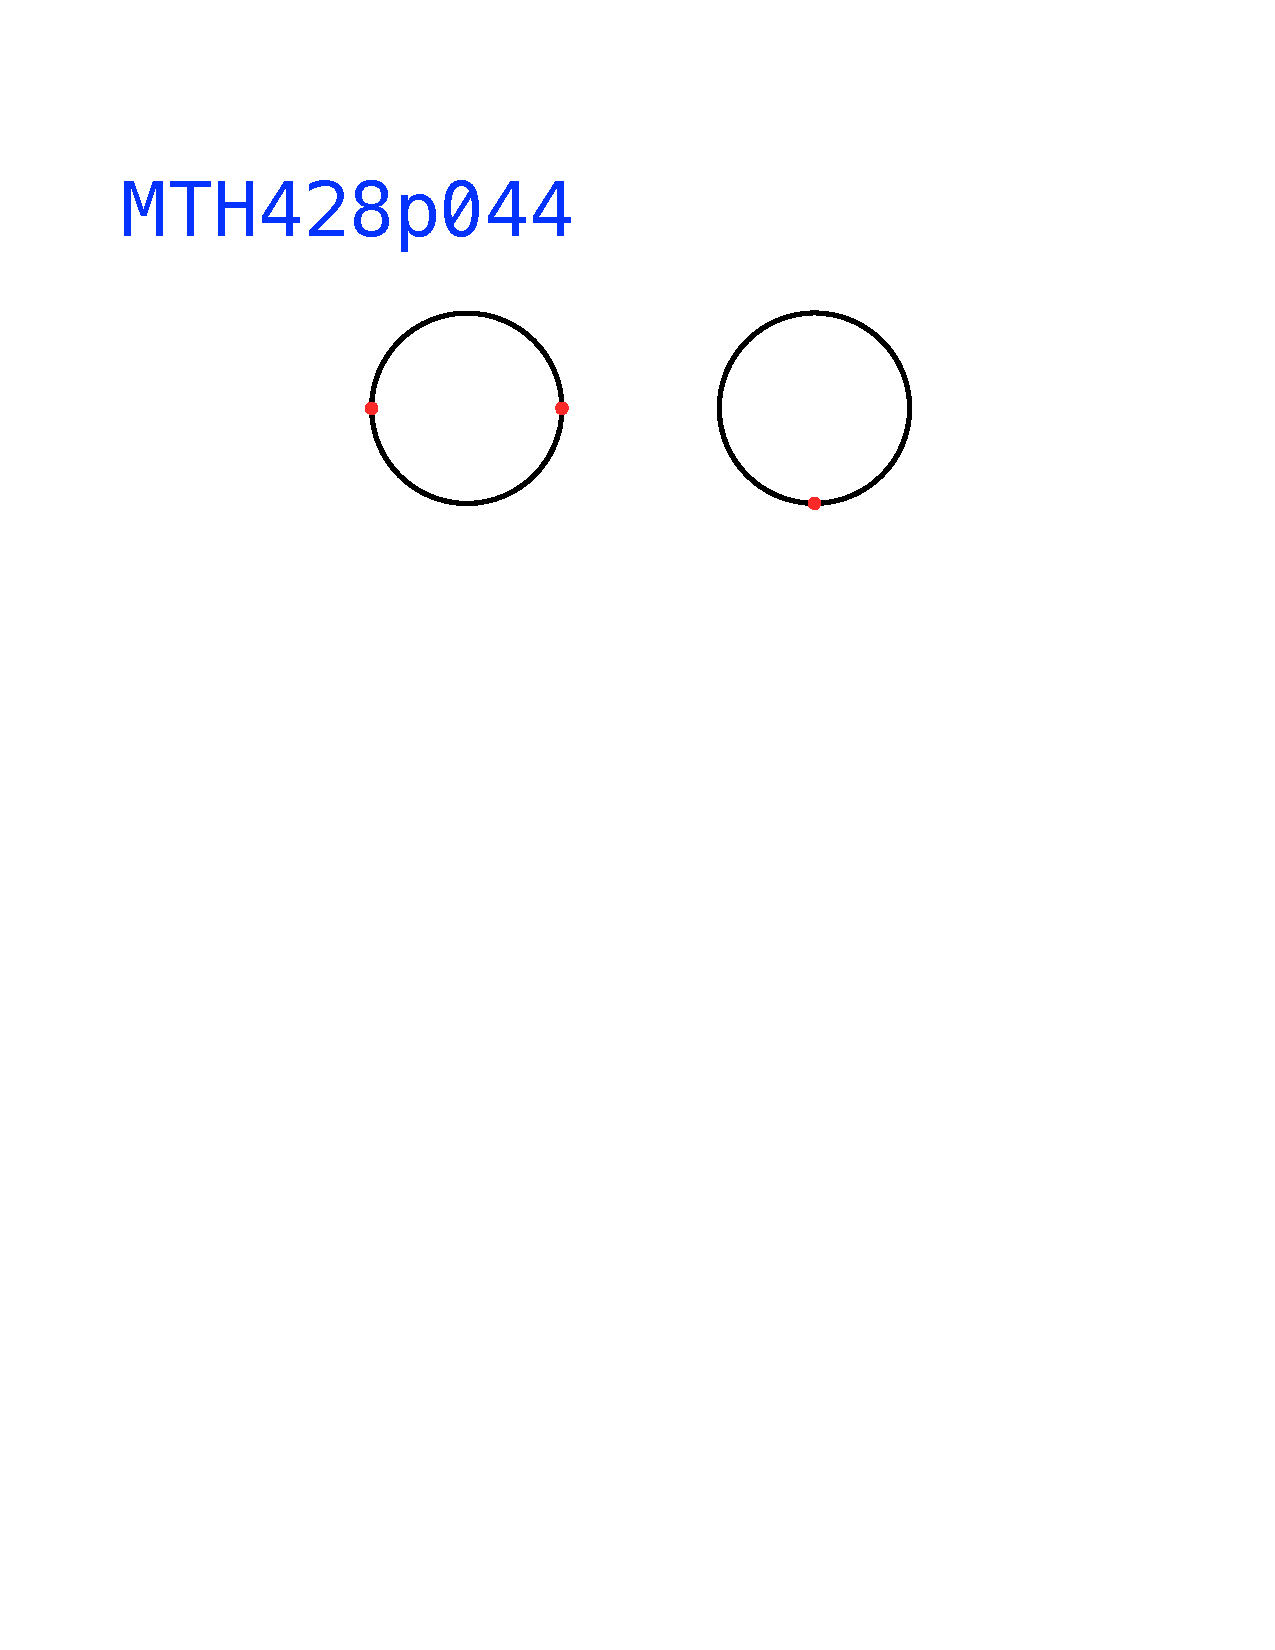
\includegraphics[width=\textwidth, trim=0mm 192mm 0mm 52mm, clip]{pictures/MTH428p044.pdf}}};

%%% COORDINATE GRID
%\draw[step=0.5, help lines] (0,0) to[grid with coordinates] (15,9);
%%% 

\node[anchor= base east]  at (4.82 , 1.32){\color{red} \small  $e^{0}_{1}$};
\node[anchor= base west]  at (7.3 , 1.32){\color{red} \small  $e^{0}_{2}$};
\node[anchor= north]  at (6.1 , 3.3){\small  $e^{1}_{1}$};
\node[anchor= north]  at (6.1 , 0.15){\small  $e^{1}_{2}$};
\node[anchor= north]  at (10.6 , 3.3){\small  $e^{1}$};
\node[anchor= north]  at (10.6 , 0.15){\color{red} \small  $e^{0}$};
\end{tikzpicture}

\end{example}

\begin{example}
Here are two examples of CW-complex structures on $S^{2}$. The first  has two cells in in each of the dimensions $0$, $1$, and $2$. The second has one $0$-cell $e^{0}$ and one $2$-cell which is attached 
using the constant attaching map $S^{1}\to e^{0}$:

\begin{tikzpicture}

\node[anchor=south west,inner sep=0] at (0,0) 
{{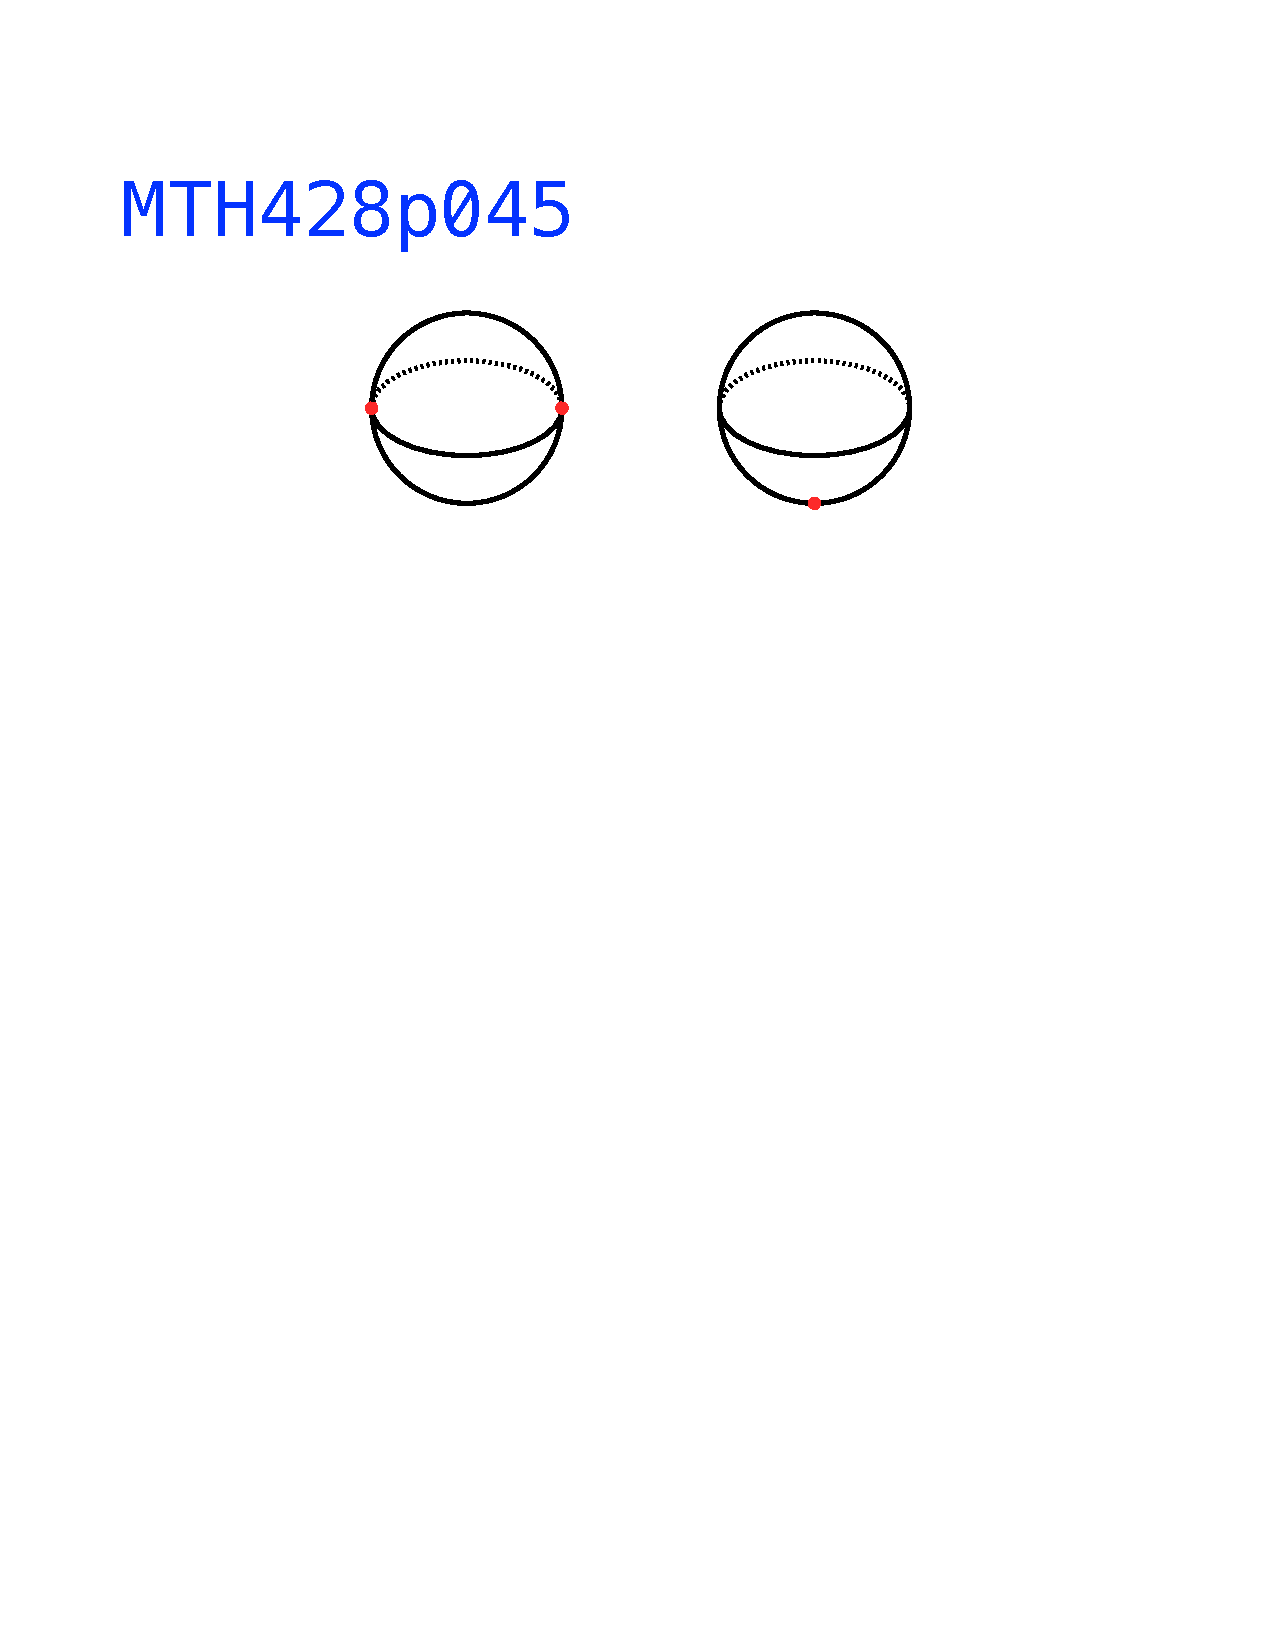
\includegraphics[width=\textwidth, trim=0mm 192mm 0mm 52mm, clip]{pictures/MTH428p045.pdf}}};

%%% COORDINATE GRID
%\draw[step=0.5, help lines] (0,0) to[grid with coordinates] (15,9);
%%% 

\node[anchor= north]  at (6.1 , 3.3){\small  $e_{1}^{2}$};
\node[anchor= north]  at (6.1 , 0.2){\small  $e^{2}_{2}$};
\node[anchor= base east]  at (4.82 , 1.32){\color{red} \small  $e^{0}_{1}$};
\node[anchor= base west]  at (7.3 , 1.32){\color{red} \small  $e^{0}_{2}$};
\node[anchor= base]  at (6.1 , 1.65){\small  $e^{1}_{1}$};
\node[anchor= base]  at (6.1 , 1.03){\small  $e^{1}_{2}$};
\node[anchor= north]  at (10.6 , 3.3){\small  $e^{2}$};
\node[anchor= north]  at (10.6 , 0.2){\color{red} \small  $e^{0}$};
\end{tikzpicture}
\end{example}

\begin{example}
The cylinder $S^{1}\times [0, 1]$ can be given a CW-complex structure with two $0$-cells, 
three $1$-cells, and one $2$-cell. It is easier to visualize this structure if we consider the cylinder 
as a quotient space obtained by gluing together two vertical edges of a square. The pair 
of the upper vertices of the square represents one $0$-cell of the cylinder, and the  pair of lower vertices 
the second  $0$-cell. The three $1$-cells come from each of the  horizontal edges and the pair of vertical 
edges. The interior of the square corresponds to the interior of the $2$-cell of the cylinder:   

%---BBLANK
\begin{tikzpicture}

\node[anchor=south west,inner sep=0] at (0,0) 
{{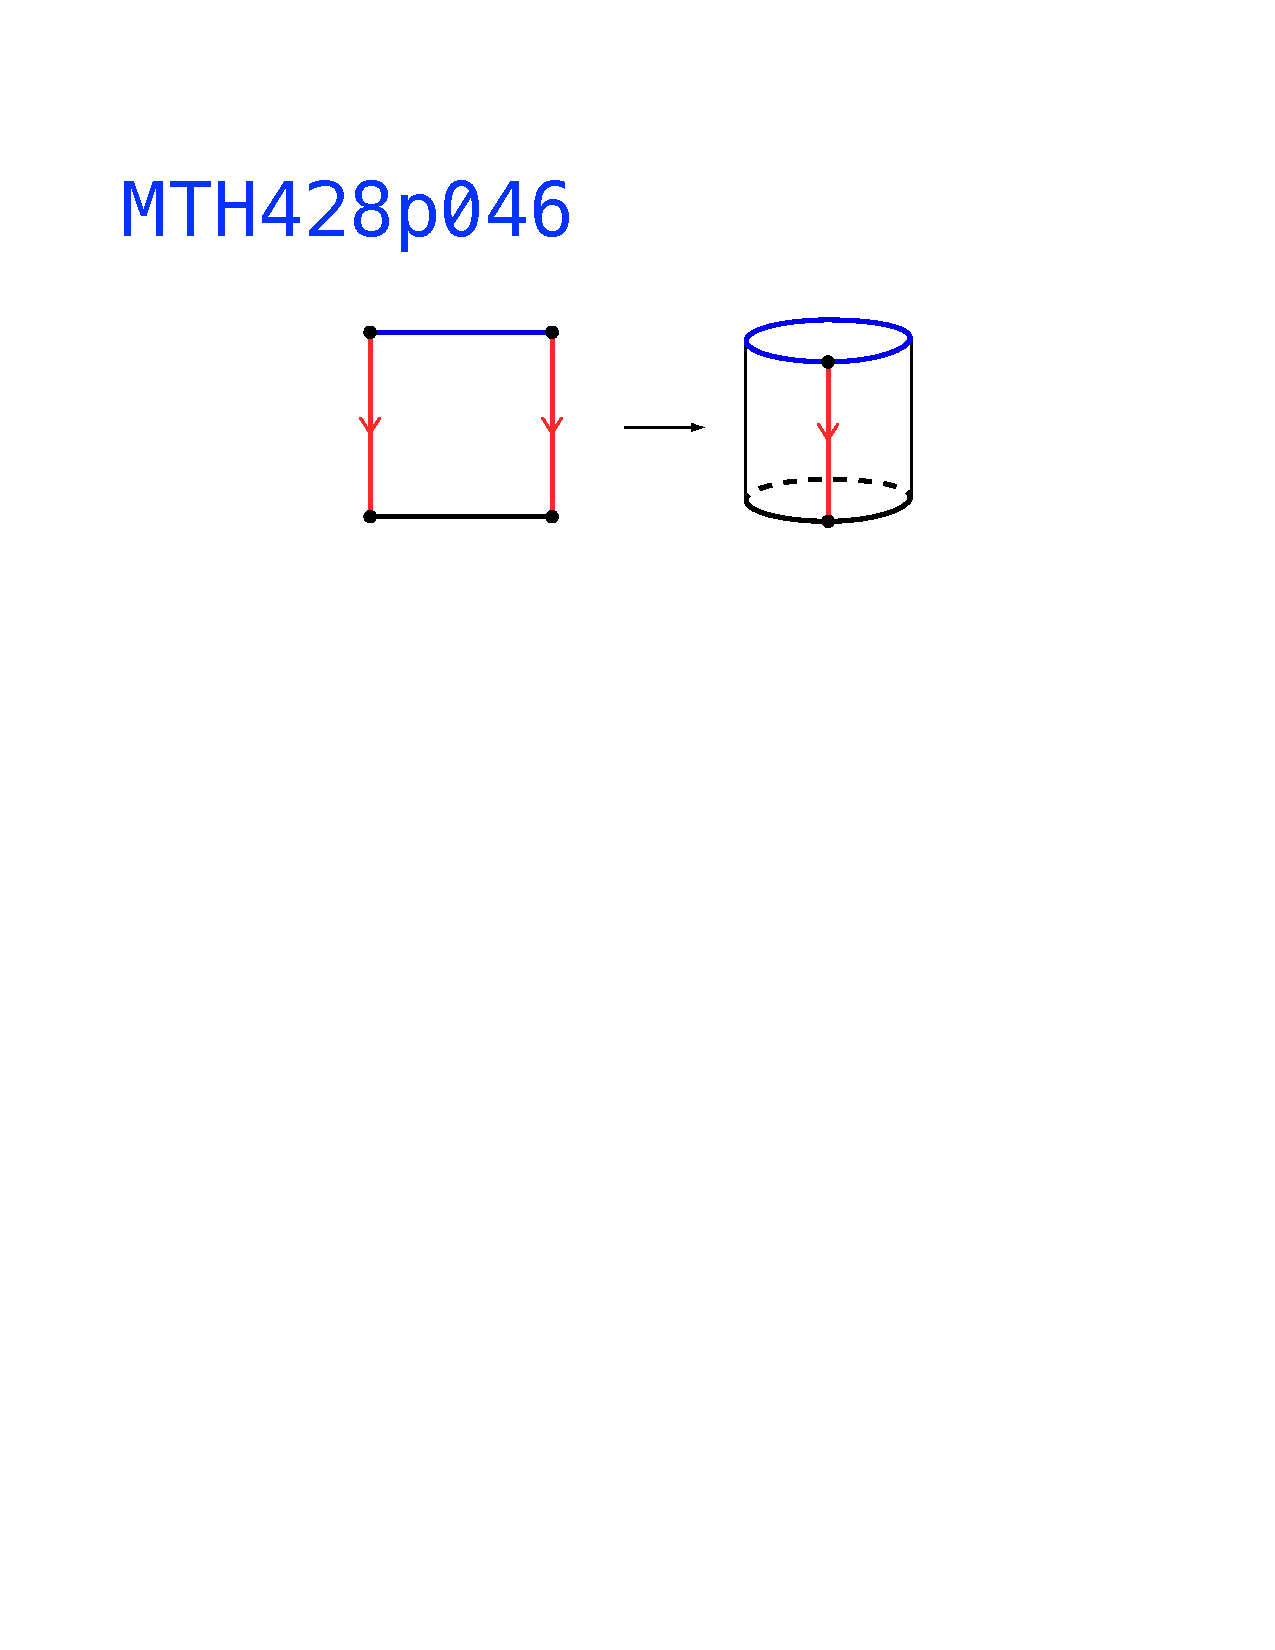
\includegraphics[width=\textwidth, trim=0mm 190mm 0mm 52mm, clip]{pictures/MTH428p046.pdf}}};

%%% COORDINATE GRID
%\draw[step=0.5, help lines] (0,0) to[grid with coordinates] (15,9);
%%% 

\node[anchor= base east]  at (4.77 , 2.55){\small  $e_{1}^{0}$};
\node[anchor= base west]  at (7.2 , 2.55){\small  $e_{1}^{0}$};
\node[anchor= base east]  at (4.77 , 0.0){\small  $e_{2}^{0}$};
\node[anchor= base west]  at (7.2 , 0.0){\small  $e_{2}^{0}$};
\node[anchor= base]  at (6.0 , 2.75){\color{blue} \small  $e^{1}_{1}$};
\node[anchor= base]  at (6.0 , -0.3){ \small  $e^{1}_{2}$};
\node[anchor= base east]  at (4.77 , 1.3){\color{red} \small  $e^{1}_{3}$};
\node[anchor= base west]  at (7.23 , 1.3){\color{red} \small  $e^{1}_{3}$};
\node[anchor= base ]  at (6.0 , 1.3){\small  $e^{2}$};

\end{tikzpicture}
%---EBLANK


Since the M\"{o}bius band, the torus, and the Klein bottle also can be constructed 
by gluing together some edges of the square we can describe CW-complex structures on these spaces 
in a similar way:

%---BBLANK
\begin{tikzpicture}

\node[anchor=south west,inner sep=0] at (0,0) 
{{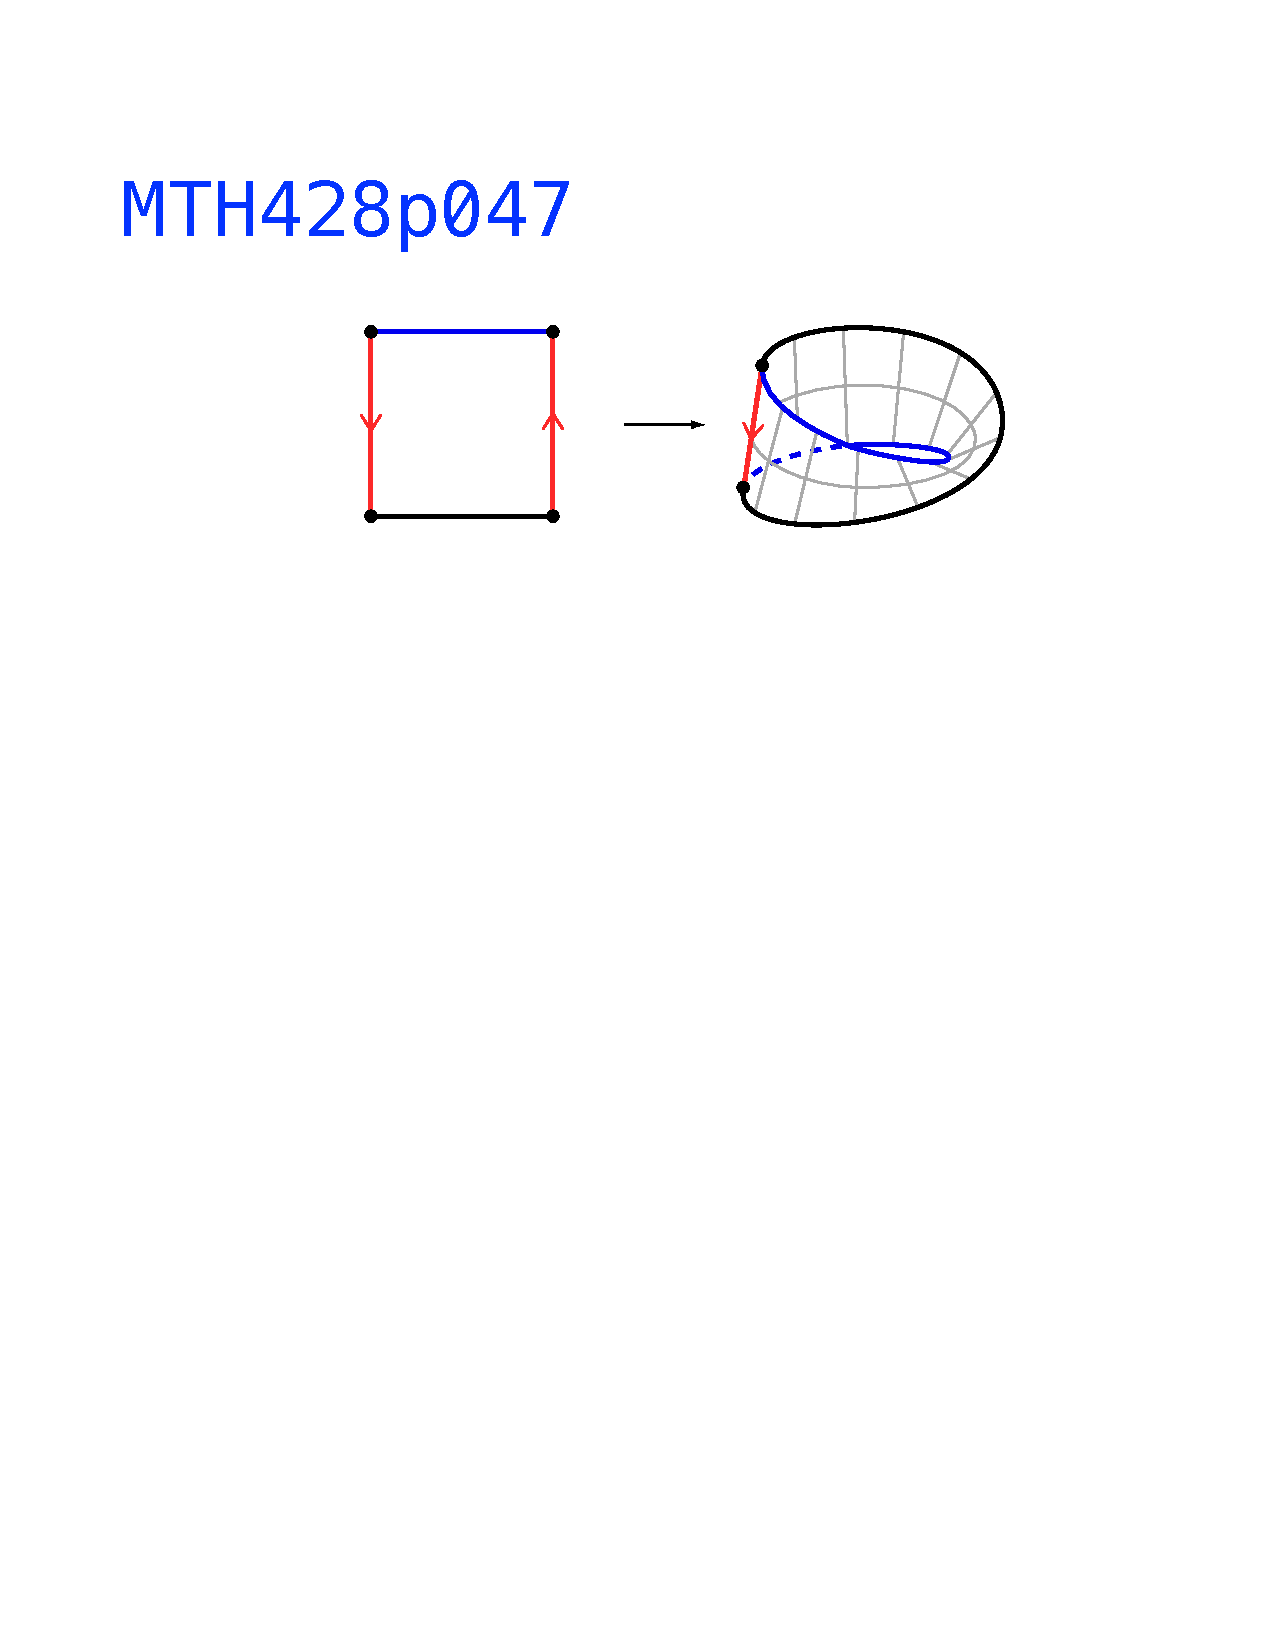
\includegraphics[width=\textwidth, trim=0mm 190mm 0mm 52mm, clip]{pictures/MTH428p047.pdf}}};

%%% COORDINATE GRID
%\draw[step=0.5, help lines] (0,0) to[grid with coordinates] (15,9);
%%% 

\node[anchor= base east]  at (4.8 , 2.55){\small  $e_{1}^{0}$};
\node[anchor= base west]  at (7.2 , 2.55){\small  $e_{2}^{0}$};
\node[anchor= base east]  at (4.8 , 0.0){\small  $e_{2}^{0}$};
\node[anchor= base west]  at (7.2 , 0.0){\small  $e_{1}^{0}$};
\node[anchor= base]  at (6.0 , 2.75){\color{blue} \small  $e^{1}_{1}$};
\node[anchor= base]  at (6.0 , -0.3){ \small  $e^{1}_{2}$};
\node[anchor= base east]  at (4.77 , 1.3){\color{red} \small  $e^{1}_{3}$};
\node[anchor= base west]  at (7.23 , 1.3){\color{red} \small  $e^{1}_{3}$};
\node[anchor= base ]  at (6.0 , 1.3){\small  $e^{2}$};

\end{tikzpicture}


\begin{tikzpicture}

\node[anchor=south west,inner sep=0] at (0,0) 
{{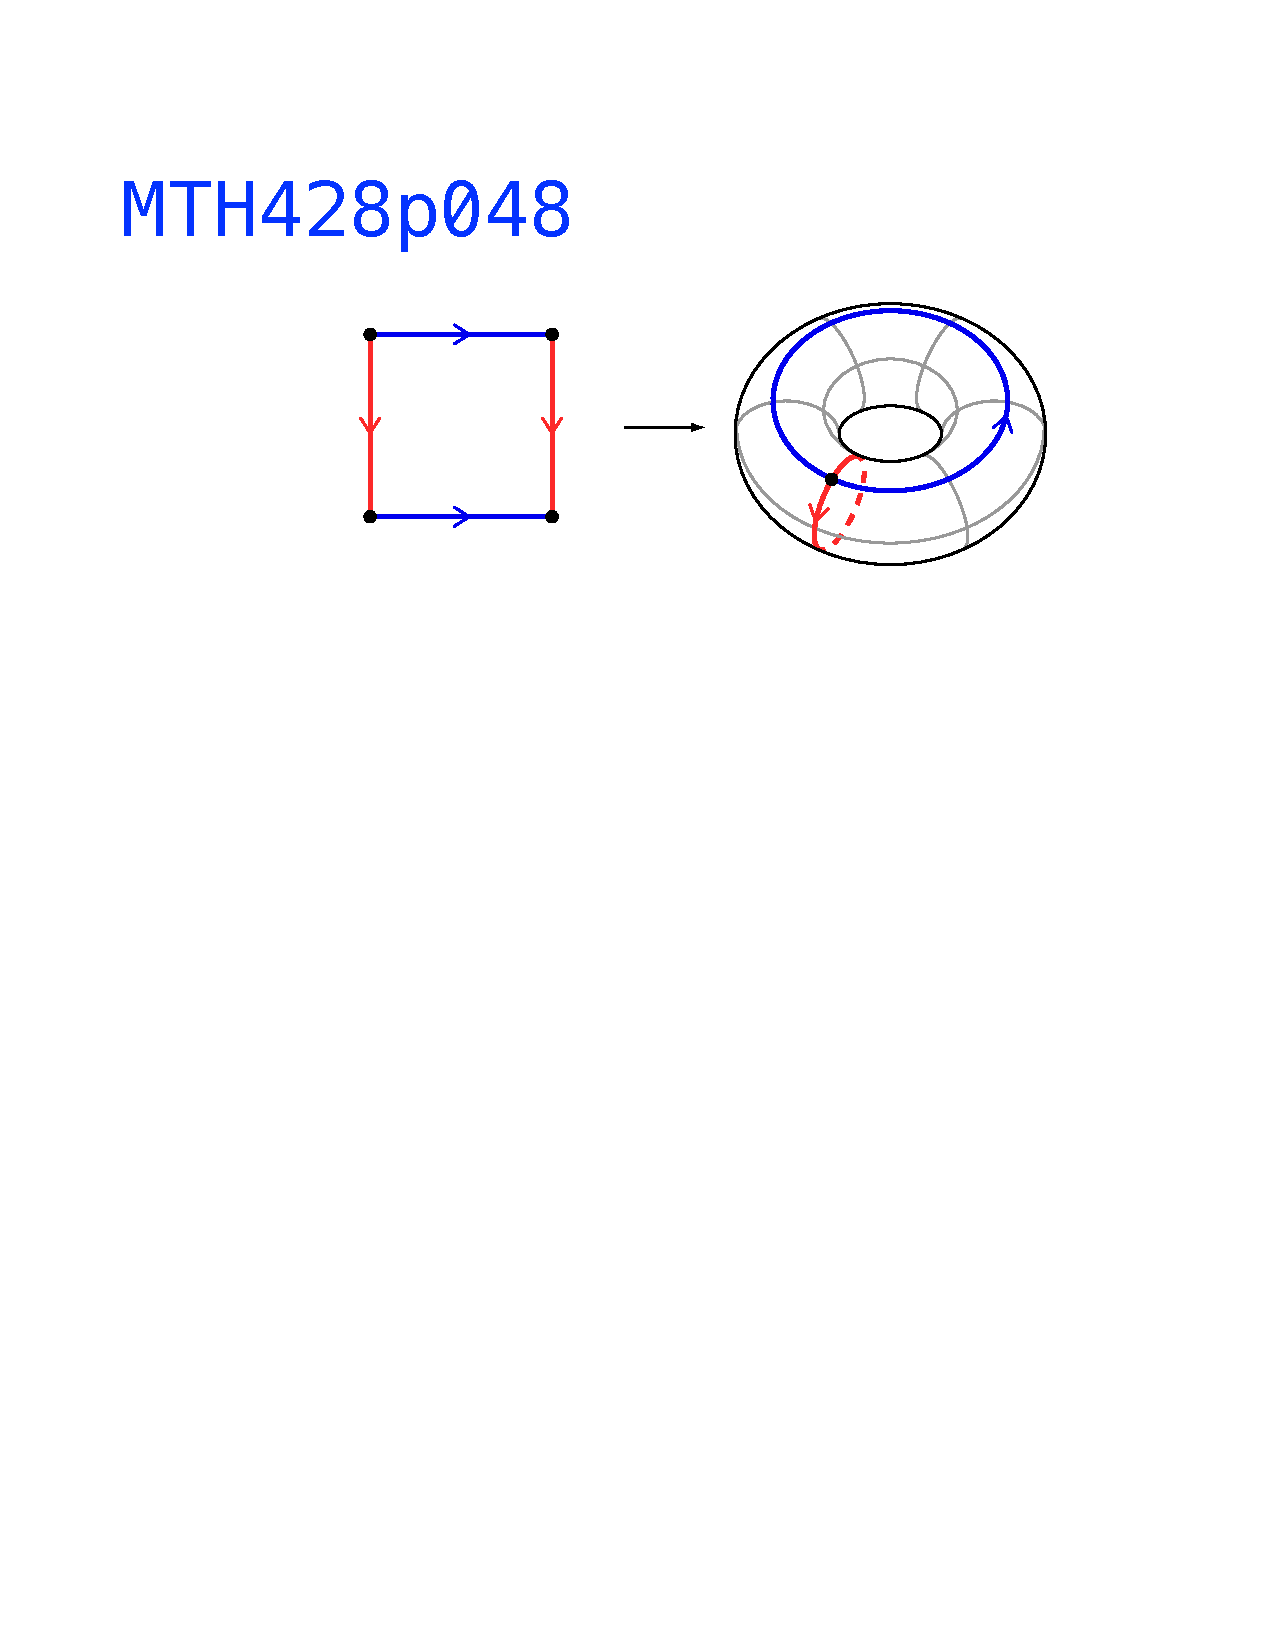
\includegraphics[width=\textwidth, trim=0mm 183mm 0mm 50mm, clip]{pictures/MTH428p048.pdf}}};

%%% COORDINATE GRID
%\draw[step=0.5, help lines] (0,0) to[grid with coordinates] (15,9);
%%% 

\node[anchor= base east]  at (4.85 , 3.05){\small  $e^{0}$};
\node[anchor= base west]  at (7.2 , 3.05){\small  $e^{0}$};
\node[anchor= base east]  at (4.8 , 0.6){\small  $e^{0}$};
\node[anchor= base west]  at (7.2 , 0.6){\small  $e^{0}$};
\node[anchor= base]  at (6.0 , 3.3){\color{blue} \small  $e^{1}_{1}$};
\node[anchor= base]  at (6.0 , 0.25){ \small \color{blue} $e^{1}_{1}$};
\node[anchor= base east]  at (4.77 , 1.8){\color{red} \small  $e^{1}_{2}$};
\node[anchor= base west]  at (7.23 , 1.8){\color{red} \small  $e^{1}_{2}$};
\node[anchor= base ]  at (6.0 , 1.8){\small  $e^{2}$};

\end{tikzpicture}



\begin{tikzpicture}

\node[anchor=south west,inner sep=0] at (0,0) 
{{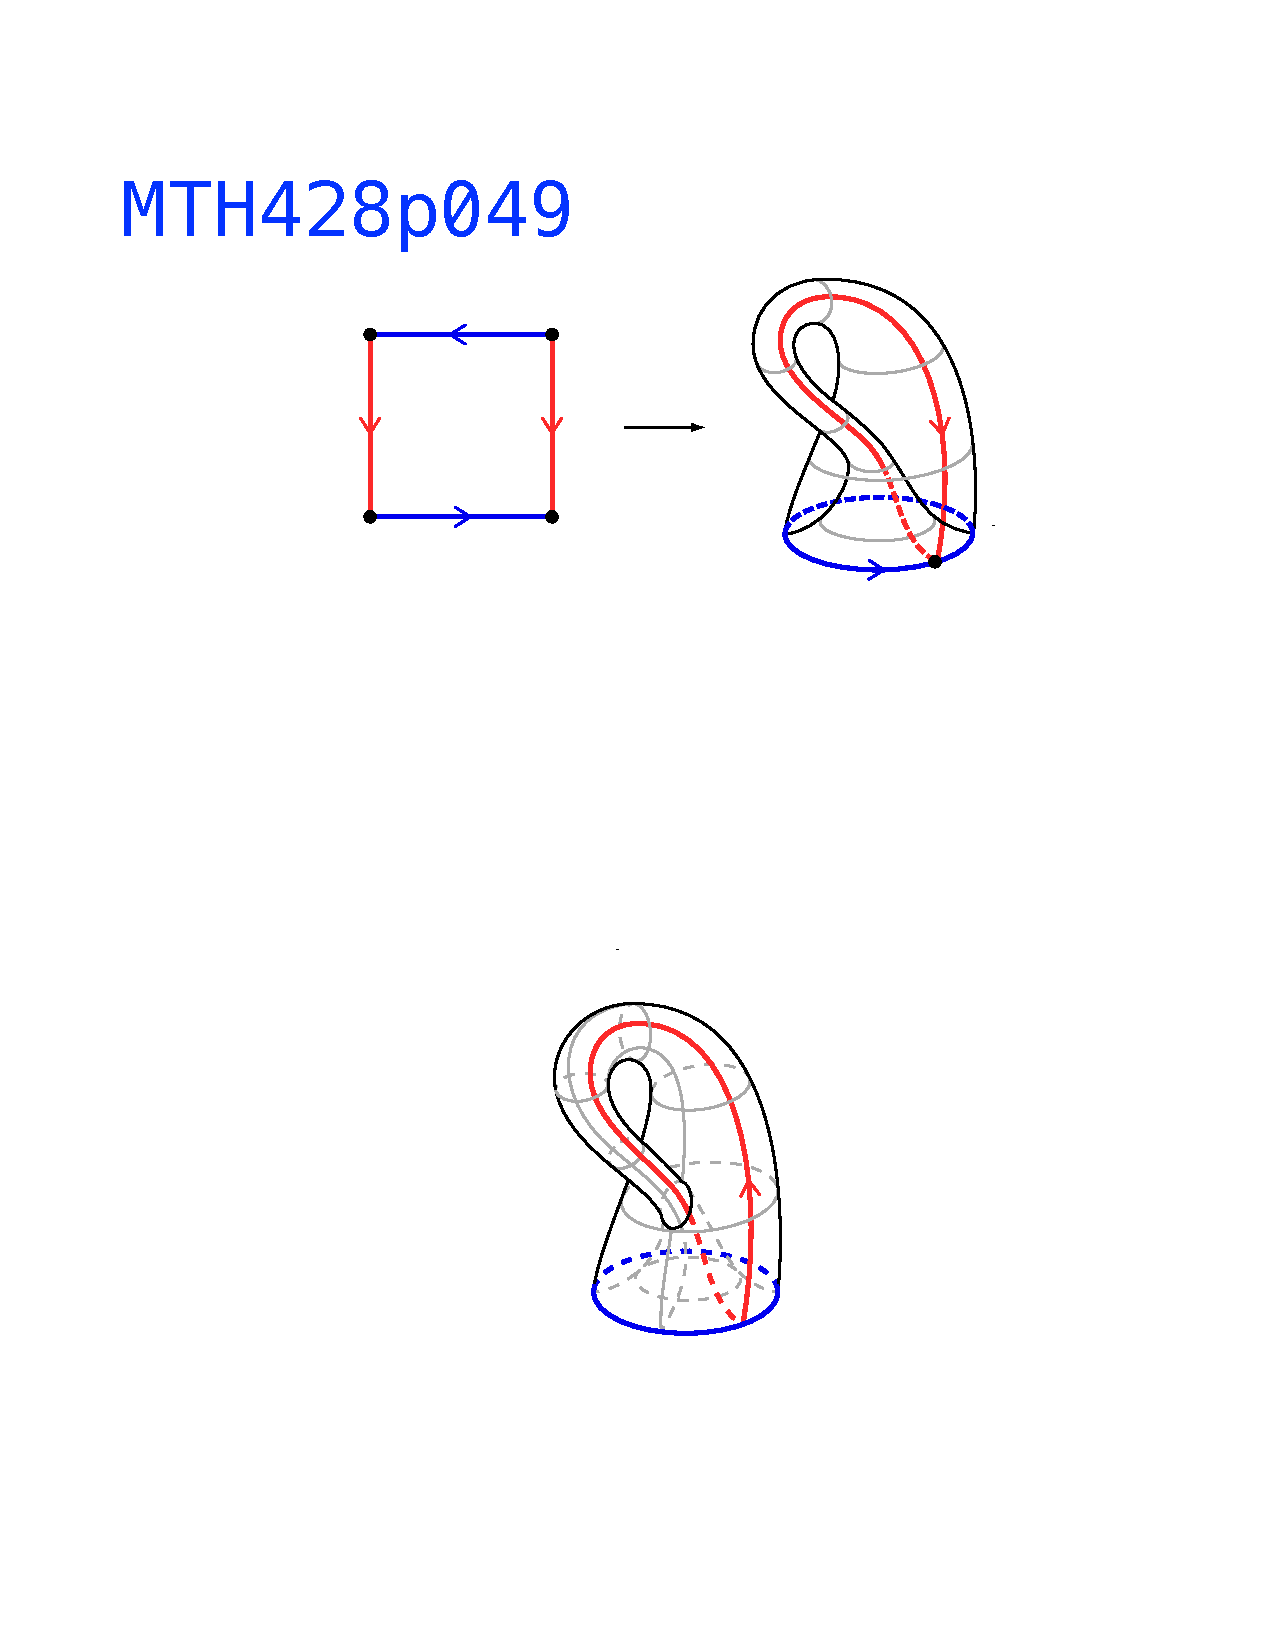
\includegraphics[width=\textwidth, trim=0mm 181mm 0mm 44mm, clip]{pictures/MTH428p049.pdf}}};

%%% COORDINATE GRID
%\draw[step=0.5, help lines] (0,0) to[grid with coordinates] (15,9);
%%% 

\node[anchor= base east]  at (4.85 , 3.2){\small  $e^{0}$};
\node[anchor= base west]  at (7.2 , 3.2){\small  $e^{0}$};
\node[anchor= base east]  at (4.8 , 0.7){\small  $e^{0}$};
\node[anchor= base west]  at (7.2 , 0.7){\small  $e^{0}$};
\node[anchor= base]  at (6.0 , 3.5){\color{blue} \small  $e^{1}_{1}$};
\node[anchor= base]  at (6.0 , 0.4){ \small \color{blue} $e^{1}_{1}$};
\node[anchor= base east]  at (4.77 , 1.9){\color{red} \small  $e^{1}_{2}$};
\node[anchor= base west]  at (7.23 , 1.9){\color{red} \small  $e^{1}_{2}$};
\node[anchor= base ]  at (6.0 , 1.9){\small  $e^{2}$};

\end{tikzpicture}
%---EBLANK # \newpage

\end{example}

\begin{example}
Recall that the $2$-dimensional real projective space $\RP^{2}$ can be constructed 
as a quotient space of the  disc $D^{2}$ obtained by identifying antipodal points 
on the boundary of $D^{2}$: $x\sim (-x)$ for  $x\in S^{1}$. This space can be 
given a CW-complex structure with one $0$-cell, one $1$-cell, and one $2$-cell:


\begin{tikzpicture}
\node[anchor=south west,inner sep=0] at (0,0) 
{{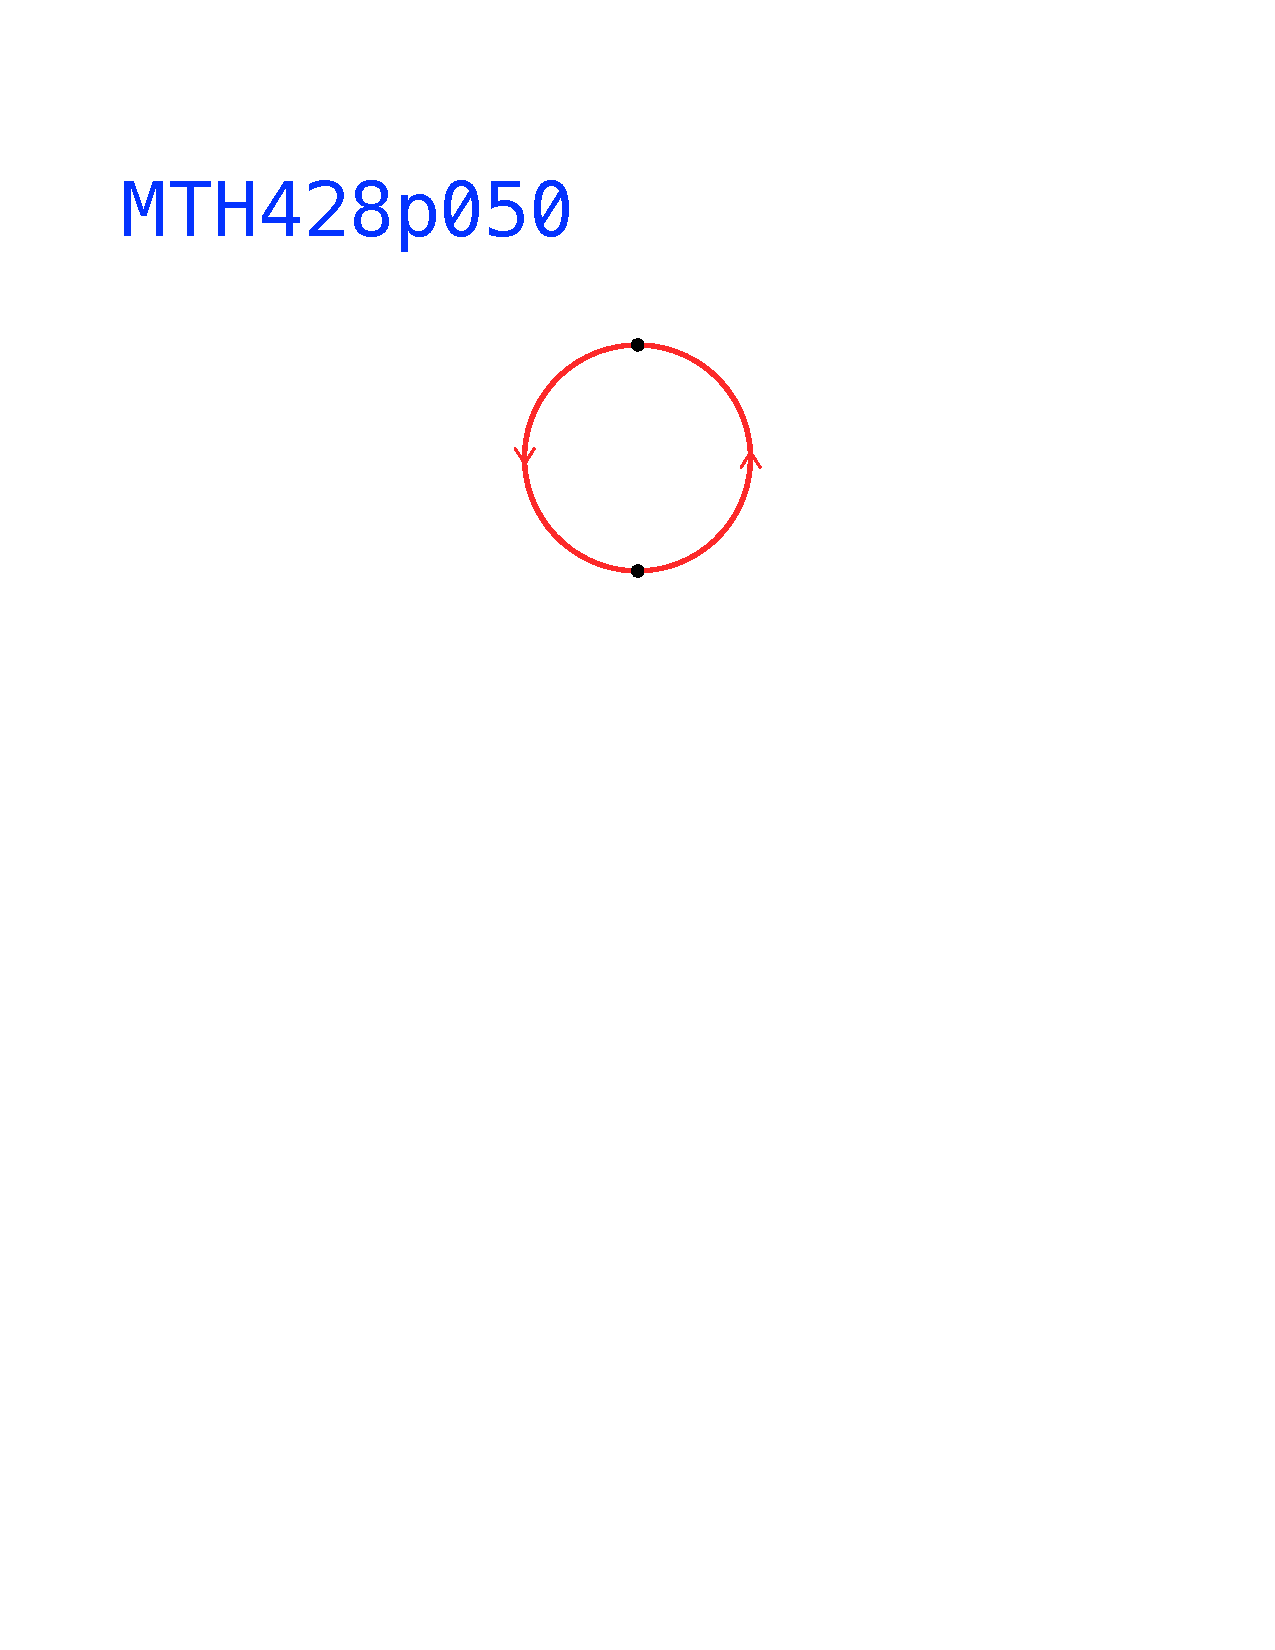
\includegraphics[width=\textwidth, trim=0mm 181mm 0mm 55mm, clip]{pictures/MTH428p050.pdf}}};

%%% COORDINATE GRID
%\draw[step=0.5, help lines] (0,0) to[grid with coordinates] (15,9);
%%% 

\node[anchor= base]  at (8.32 , 3.25){\small  $e^{0}$};
\node[anchor= base]  at (8.32 , -0.32){\small  $e^{0}$};
\node[anchor= base east]  at (6.75 , 1.57){\color{red} \small  $e^{1}$};
\node[anchor= base west]  at (9.8 , 1.57){\color{red} \small  $e^{1}$};
\node[anchor= base ]  at (8.32 , 1.57){\small  $e^{2}$};
\end{tikzpicture}


\end{example}

%---BBLANK
\begin{note}
It is not true that every space can be given a structure of a CW-complex. 
%---EBLANK # \end{note} \newpage
For example, 
consider the following subspace of the real line:
$$X = \{\tfrac{1}{n} \in \R \ | \ n = 1, 2, \dots \} \cup \{0\}$$
This space is not homeomorphic or even homotopy equivalent to a $CW$-complex.
To show this we will use the fact that if $Y$ is a CW-complex then each path connected component of $Y$
is open in $Y$ (exercise). Assume  that there exists a homotopy equivalence $f\colon X \to Y$ where 
$Y$ is a CW-complex. This implies that the induced map $f_{\ast}\colon \pi_{0}(X) \to \pi_{0}(Y)$
is a bijection. On the other hand let $\{Y_{i}\}_{i\in I}$ be the family of all path connected components 
of $Y$. The sets $Y_{i}$ are open in $Y$, so the sets $f^{-1}(Y_{i})$ are open in $X$ 
and they define an open cover of $X$.  The space $X$ is compact, so this cover has a finite subcover 
$\{f^{-1}(Y_{i_{1}}), \dots, f^{-1}(Y_{i_{k}})\}$. Since $X$ is an infinite space this implies that that 
there exist distinct points  $x_{1}, x_{2}\in X$ such that $f(x_{1})$ and $f(x_{2})$
belong to the same path connected component of $Y$. On the other hand $x_{1}$ and $x_{2}$
belong to different path connected components in $X$ since every path connected component of $X$
consists of a single point. This shows that $f_{\ast}\colon \pi_{0}(X) \to \pi_{0}(Y)$ is not a bijection, 
and so we obtain a contradiction. 


\end{note}


The following fact if often useful: 


%---BBLANK
\begin{proposition}
\label{COMPACT CW COMPLEX PROP}
Let $X$ be a CW-complex. A set $A\subseteq X$ is compact if and only if $A$ is closed and $A$ has 
a non-empty intersection with  finitely many open cells of $X$ only.  
\end{proposition}

\begin{proof}
Exercise. 
\end{proof}
%---EBLANK # \vskip 40mm


%---BBLANK
\begin{corollary}
\label{FINITE CW COMPACT COR}
A CW-complex is compact if and only if it is a finite. 
\end{corollary}
%---EBLANK # \newpage


\begin{proof}
Follows from Proposition \ref{COMPACT CW COMPLEX PROP}
\end{proof}




%%%%%%%%%%%%%%%%%%%%%%%%%%%%%%%
%  EXERCISES
%%%%%%%%%%%%%%%%%%%%%%%%%%%%%%%

\exercises

\begin{exercise}
Show that a CW-complex $X$ is path connected if and only if its 1-skeleton $X^{(1)}$ is path connected. 
\end{exercise}

\begin{exercise}
Prove Proposition \ref{COMPACT CW COMPLEX PROP}. 
\end{exercise}

\begin{exercise}
Let $X$ be a space, and let $Y = X \cup_{f} e^{n}$ be obtained by attaching one $n$-dimensional cell to $X$. 
Show that if $X$ is a retract of $Y$ then $Y \simeq X \vee S^{n}$. 
\end{exercise}


\newpage
%%%%%%%%%%%%%%%%%%%%%%%%%%%%%%%
%%%%%%%%%%%%%%%%%%%%%%%%%%%%%%%
%%%
%%%  HOMOTOPY EXTENSION PROPERTY
%%%
%%%%%%%%%%%%%%%%%%%%%%%%%%%%%%%
%%%%%%%%%%%%%%%%%%%%%%%%%%%%%%%

%---BBLANK
\chapter[Homotopy Extension Property]{Homotopy Extension \\ Property}
%---EBLANK
\chaptermark{Homotopy Extension Property}
\label{HEP CHAPTER}
\thispagestyle{firststyle}


In this chapter we begin work toward computing fundamental groups of CW-complexes.  Since 
a 0-dimensional CW-complex is a discrete space, the fundamental group of any such complex is trivial. 
The first non-trivial case we will develop a formula for the fundamental group of a  CW-complex of 
dimension 1.  Our main tool will be the homotopy extension property, which is one of the most important 
notions of algebraic topology. 

%---BBLANK
\begin{definition}
Let $X$ be a topological space, and let $A\subseteq X$. The pair $(X, A)$ has the 
\emph{homotopy extension property} if any map 
$$h\colon X\times \{0\} \cup A\times [0, 1] \to Y$$
can be extended to a map $\bar{h}\colon X \times [0, 1] \to Y$.  
\end{definition}
%---EBLANK # \vskip 50mm

The following proposition is often useful when we want to verify that the homotopy extension property holds for 
a given pair of $(X, A)$:


%---BBLANK
\begin{proposition}
\label{HEP RETRACT PROP}
A pair $(X, A)$ has the homotopy extension property if and only if $X\times \{0\} \cup A\times [0, 1]$
is a retract of $X\times [0, 1]$.
\end{proposition}

\begin{proof}
Exercise. 
\end{proof}
%---EBLANK # \newpage


The next fact implies that the homotopy extension property does not hold for arbitrary pairs of spaces:

%---BBLANK
\begin{proposition}
If a pair $(X, A)$ has the homotopy extension property and $X$ is a Hausdorff space then $A$ is closed in $X$. 
\end{proposition}

\begin{proof}
Exercise. 
\end{proof}
%---EBLANK # \vskip 40mm

%---BBLANK
\begin{proposition}
\label{CONTR QUOTIENT WITH HEP PROP}
If a pair $(X, A)$ has the homotopy extension property and the space $A$ is contractible then the quotient map 
$q\colon X \to X/A$ is a homotopy equivalence. 
\end{proposition}

\begin{proof}
Exercise
\end{proof}
%---EBLANK # \vskip 50mm

\begin{example}
In Example \ref{MAPCONECYL EX} we have shown that the space $X$ consisting of a circle and its diagonal 
is homotopy equivalent to a wedge of two circles:

\begin{equation*}
\begin{tikzpicture}[scale = 0.6]
\draw[line width = 1.6pt] (0,0) circle (1);
\draw[line width = 1.6pt] (-1, 0) -- (1, 0);
\draw[line width = 1.6pt] (6,1) circle (1);
\draw[line width = 1.6pt] (6,-1) circle (1);
\node[anchor = base] at (3,0) { $\simeq$};
\end{tikzpicture}
\end{equation*}


We can obtain the same result as follows. Let $A\subseteq X$ be the diagonal of the circle (together with its enpoints). 
It will follow from Theorem \ref{HEP REL CW THM} that the pair $(X, A)$ has the homotopy extension property. 
Since the space $A$ is contractible, using Proposition \ref{CONTR QUOTIENT WITH HEP PROP} we get a 
homotopy equivalence $X \simeq X/A$. It remains to notice that $X/A$ is homeomorphic to $S^{1}\vee S^{1}$.
\end{example}



%---BBLANK 
\begin{example}
%---EBLANK # Warsaw Curve:
Here is an example which shows that Proposition \ref{CONTR QUOTIENT WITH HEP PROP} is not true 
in general, if $(X, A)$ does not have the homotopy extension property.  
The \emph{Warsaw circle} is a subspace $W$ of $\R^{2}$ consisting of three subsets:
$$W = A\cup B \cup C$$
where:
\begin{itemize}
\item[-] $A$ is a segment of the $y$-axis: 
$$A = \{(0, y) \in \R^{2} \ | \  -1\leq y \leq 1 \}$$
\item[-] $B$ is a part of the graph of the function $f(x) = \sin\left(\frac{1}{x}\right)$: 
$$\textstyle B = \{ (x, \sin\left(\frac{1}{x}\right)) \in \R^{2} \ | \  0 < x \leq \frac{1}{2\pi} \}$$
\item[-] $C$ is an arc joining points $(0, -1)\in A$ and $(\frac{1}{2\pi}, 0)\in B$, and disjoint from 
$A\cup B$ at all other points. 
\end{itemize}

%---BBLANK 
\begin{equation*}
\begin{tikzpicture}[scale =0.75] 
\draw[red, line width = 1.5] (2.1, -1.03) -- (2.1, 1.03);
\begin{scope}
\draw[xscale=15, line width = 1.5 , domain= 0.151:0.40123,smooth,variable=\x, samples = 400] plot ({\x},{sin(pow(\x, -2) r)});
\end{scope}
\draw[blue, line width = 1.5] (2.1, -1.03) arc [radius = 2.0772, start angle = 180, end angle = 388.15];
\node at (1.8, 0.88){\small $\color{red} A$};
\node at (5.95, 0.88){\small $B$};
\node at (5.85, -2.88){\small $\color{blue} C$};
\end{tikzpicture}
\end{equation*}
%---EBLANK

Consider the pair $(W, A)$. One can show that the quotient space $W/A$ is homeomorphic to 
the circle $S^{1}$ (exercise), so in particular $\pi_{1}(W/A)\cong \Z$. On the other hand, 
$\pi_{1}(W)\cong \{1\}$ (exercise). Therefore $W/A$ is not homotopy equivalent to $W$. 
  
 %---BBLANK
\end{example}
%---EBLANK  # \newpage


 %---BBLANK
\begin{theorem}
\label{HEP REL CW THM}
Any relative CW-complex $(X, Y)$ has the homotopy extension property. 
\end{theorem}
%---EBLANK  # \vskip 30mm


 %---BBLANK
\begin{lemma}
\label{DN SN-1 HEP LEMMA}
For any $n> 0$  the pair $(D^{n}, S^{n-1})$ has the homotopy extension property. 
\end{lemma}
%---EBLANK  # \vskip 40mm

While it is not difficult to prove Lemma \ref{DN SN-1 HEP LEMMA} directly, we will show that it 
follows from a more general fact.  Recall (\ref{MAP CYL CONE DEF}) that for a map $f\colon X\to Y$ the mapping cylinder of $f$ is the space $M_{f} = (X \times [0, 1] \sqcup Y) /{\sim}$ where  $(x, 1) \sim f(x)$ for all $x\in X$. Notice that the space $X$ is homeomorphic with the subspace $X\times \{0\} \subseteq M_{f}$. 



 %---BBLANK
\begin{proposition}
\label{MAP CYL HEP PROP}
For any continuous function $f\colon X \to Y$ the pair $(M_{f}, X\times \{0\})$ has the homotopy extension property. 
\end{proposition}

\begin{proof}
Exercise. 
\end{proof}
%---EBLANK  # \vskip 30mm


 %---BBLANK
\begin{proof}[Proof of Lemma \ref{DN SN-1 HEP LEMMA}]
%---EBLANK  # \ \vskip 50mm \end{proof} \newpage
Let $c\colon S^{n-1} \to \{\ast\}$ be the constant function. We have a homeomorphism 
$f \colon M_{c} \to D^{n}$ given by $f(x, t) = (1-t)x$. Moreover, $f(S^{n-1}\times \{0\}) = S^{n-1}\subseteq D^{n}$. Since by Proposition \ref{MAP CYL HEP PROP} the pair $(M_{c}, S^{n-1}\times \{0\})$ has the homotopy extension property it follows that $(D^{n}, S^{n-1})$ also has this property. 
\end{proof}

 %---BBLANK
\begin{lemma}
\label{HEP CELL ATTACHMENT LEMMA}
Let $Y$ be any space an let $X = Y\cup\{e^{n}_{\alpha}\}_{\alpha \in I}$ be a space obtained from 
by attaching some number of $n$-cells to $X$. Then the pair $(X, Y)$ has the homotopy 
extension property.   
\end{lemma}
%---EBLANK   # \newpage

\begin{proof}
To simplify notation we will assume that $X$ is obtained from $Y$ by attaching a single 
$n$-cell: $X = Y\cup e^{n}$. The proof in the general case is essentially the same. 
By Proposition \ref{HEP RETRACT PROP} it will suffice to show that   
$X\times \{0\} \cup Y\times [0, 1]$ is a retract of $X\times [0, 1]$. 
Let $f \colon S^{n-1} \to Y$ be the attaching map of the cell $e^{n}$.
We have a homeomorphisms
$$X\times [0, 1]\simeq (D^{n}\times [0, 1] \sqcup Y\times [0, 1])/\!\sim$$ 
and 
$$X\times \{0\} \cup Y\times [0, 1] \simeq ((  D^{n}\times \{0\} \cup S^{n-1}\times [0, 1]) \sqcup Y\times [0, 1]) /\!\sim$$
where $(x, t)\sim (f(x), t)$ for $x\in S^{n-1}$.
By Lemma \ref{DN SN-1 HEP LEMMA} there is a retraction 
$$r\colon D^{n}\times [0, 1] \to  D^{n}\times \{0\} \cup S^{n-1}\times [0, 1]$$
The map 
$$r\sqcup \id_{Y\times [0, 1]} \colon ((  D^{n}\times \{0\} \cup S^{n-1}\times [0, 1]) \sqcup Y\times [0, 1]) /\!\sim
\ \to \ (D^{n}\times [0, 1] \sqcup Y\times [0, 1])/\!\sim$$
gives the desired retraction $X\times [0, 1] \to X\times \{0\} \cup Y\times [0, 1]$. 
\end{proof}


\begin{proof}[Proof of Theorem \ref{HEP REL CW THM}]
Recall (\ref{RELCW DEF}) that if $(X, Y)$ is a relative $CW$-complex then $X = \bigcup_{n=-1}^{\infty} X^{(n)}$
where $X^{(-1)} = Y$ and for $n\geq 0$ the subspace of $X^{(n)}\subseteq X$ obtained by attaching 
$n$-cells to $X^{(n-1)}$. By Lemma \ref{HEP CELL ATTACHMENT LEMMA} for each $n\geq 0$
there exists a retraction 
$$r_{n}\colon X^{(n)}\times [0, 1] \to X^{(n)}\times \{0\} \cup X^{(n-1)}\times [0, 1]$$
We can extend $r_{n}$ to a map 
$$\xov{r}_{n}\colon X\times \{0\} \cup X^{(n)}\times [0, 1] \to X \times \{0\} \cup X^{(n-1)}\times [0, 1]$$
by setting $\xov{r}_{n}(x, 0) = (x, 0)$ for $x\in X$. 
Define:
$$r\colon X \times [0, 1] \to X\times \{0\} \cup Y\times [0, 1]$$
by $r(x, t) = \xov{r}_{0}\circ \xov{r}_{1}\circ{\dots} \circ \xov{r}_{n}(x, t)$ if $x\in X^{(n)}$, $n\geq 0$,  and $r(x, t) = (x, t)$
if $x\in X^{(-1)} = Y$.  One can check that $r$ is a well defined, continuous retraction (exercise). 

\end{proof}

 %---BBLANK
\begin{theorem}
\label{FINCWDIM1HOTYPE THM}
If $X$ is a  path connected finite CW-complex of dimension $1$ then $X \simeq \bigvee_{i=1}^{n} S^{1}$
where 
$$n = \begin{pmatrix}
\text{number of} \\[1mm]
\text{1-cells of $X$} \\
\end{pmatrix}
- 
\begin{pmatrix}
\text{number of} \\[1mm]
\text{0-cells of $X$} \\
\end{pmatrix}
+1
$$
\end{theorem}
%---EBLANK   # \vskip 30mm

 %---BBLANK
\begin{corollary}
If $X$ is a  path connected finite CW-complex of dimension $1$  then 
$\pi_{1}(X) \cong \ast_{i=1}^{n}\Z$
where $n$ is defined as in Theorem \ref{FINCWDIM1HOTYPE THM}.
\end{corollary}
%---EBLANK   # \newpage

\begin{proof}
This follows from Theorem \ref{FINCWDIM1HOTYPE THM} and Example \ref{PI1S1VS1 EXAMPLE}.  
\end{proof}

\begin{proof}[Proof of Theorem \ref{FINCWDIM1HOTYPE THM}]
We will argue by induction with respect to the number $k$ of $0$-cells in $X$. If $k=1$
then the statement is obvious. Assume then that the statement of theorem is true for  
all complexes whose number of $0$-cells is $k$, and let $X$ be a path connected 
finite $1$-dimensional CW-complex whose set of $0$-cells is $\{x_{1}, x_{2}, \dots, x_{k+1}\}$
for some $k\geq 1$. Since $X$ is path connected 
there exists a $1$-cell $e$ in $X$  that joins $x_{1}$ with some other $0$-cell $x_{i}$. 
Let $A$ denote the subcomplex of $X$ consisting of the cells $x_{1}$, $x_{i}$ and $e$. 
Notice that $A$ is homeomorphic to the closed interval $[0, 1]$.
The pair $(X, A)$ is a relative CW-complex, so by Theorem \ref{HEP REL CW THM}
it satisfies the homotopy extension property. Since $A$ is contractible, by  
Proposition \ref{CONTR QUOTIENT WITH HEP PROP} the quotient map 
$q\colon X \to X/A$ is a homotopy equivalence.  

\begin{equation*}
\begin{tikzpicture}[
    scale = 1.7,
    d0/.style = {line width = 1.6pt}
]


%left picture
\begin{scope}
\draw[d0] (0,0) -- (1,0) -- (0.5, {sqrt(3)/2 - 0.1}) -- cycle;
\draw[d0] (1,0) -- (1.6,0);
\draw[d0] (0,0) ..controls +(0.4, -0.3) and +(-0.4, -0.3).. (1,0);

\begin{scope}[shift={(0.5,{sqrt(3)/2 -0.1})}]
\draw[d0, scale=0.15, rotate=90]
(0,0) .. controls (0,0) and (1,1) .. 
(2, 1) .. controls (2.5,1) and (3, 0.5).. 
(3,0)  ..controls (3, -0.5) and (2.5, -1)..  
(2,-1) ..controls (1, -1) and (0,0).. 
cycle;
\end{scope}

\draw[d0, scale=0.15, rotate=180]
(0,0) .. controls (0,0) and (1,1) .. 
(2, 1) .. controls (2.5,1) and (3, 0.5).. 
(3,0)  ..controls (3, -0.5) and (2.5, -1)..  
(2,-1) ..controls (1, -1) and (0,0).. 
cycle;

\draw[d0, red] (1, 0) -- node[anchor=south west, xshift = -1pt] {\small $e$}(0.5, {sqrt(3)/2 - 0.1});

\filldraw[] (0,0) circle (0.05);
\filldraw[red] (1,0) circle (0.05) node[anchor = north, xshift = 2pt, yshift=-2pt] {\small $x_{1}$};
\filldraw[] (1.6,0) circle (0.05);
\filldraw[red] (0.5, {sqrt(3)/2 - 0.1}) circle (0.05) node[anchor = east, xshift = -2pt] {\small $x_{i}$};
\end{scope}


%right picture
\begin{scope}[shift = {(4,0)}]
\draw[d0] (0,0) -- (1,0);
\draw[d0] (1,0) -- (1.6,0);
\draw[d0] (0,0) ..controls +(0.4, -0.3) and +(-0.4, -0.3).. (1,0);
\draw[d0] (0,0) ..controls +(0.4, 0.3) and +(-0.4, 0.3).. (1,0);

\begin{scope}[shift={(1,0)}]
\draw[d0, scale=0.15, rotate=90]
(0,0) .. controls (0,0) and (1,1) .. 
(2, 1) .. controls (2.5,1) and (3, 0.5).. 
(3,0)  ..controls (3, -0.5) and (2.5, -1)..  
(2,-1) ..controls (1, -1) and (0,0).. 
cycle;
\end{scope}

\draw[d0, scale=0.15, rotate=180]
(0,0) .. controls (0,0) and (1,1) .. 
(2, 1) .. controls (2.5,1) and (3, 0.5).. 
(3,0)  ..controls (3, -0.5) and (2.5, -1)..  
(2,-1) ..controls (1, -1) and (0,0).. 
cycle;


\filldraw[] (0,0) circle (0.05);
\filldraw[red] (1,0) circle (0.05);
\filldraw[] (1.6,0) circle (0.05);
\end{scope}


\draw[thick, ->, >=latex] (2.2, 0) -- node[anchor=south] {\small $q$} node[anchor=north] {\small $\simeq$}(3.0, 0);


\end{tikzpicture}
\end{equation*}

The space $X/A$ has the structure of a  1-dimensional  CW-complex 
with one 0-cell and one 1-cell less than $X$. Therefore, by the inductive assumption 
the statement of the theorem holds for $X/A$, and so it also holds for $X$. 


\end{proof}



 %---BBLANK
Theorem \ref{FINCWDIM1HOTYPE THM} can be generalized to infinite 1-dimensional complexes:

\begin{theorem}
 If $X$ is a path connected $1$-dimensional CW-complex then $X\simeq  \bigvee_{I\in I} S^{1}$ for some 
set $I$. As a consequence $\pi_{1}(X) \cong \ast_{i\in I} \Z$.  
\end{theorem}


 %---EBLANK # \vskip 40mm

 %---BBLANK
\begin{note}
 %---EBLANK # Euler characteristic. \end{note} \newpage
For a finite CW-complex $X$, let $c_{n}(X)$ denote the number of $n$-cells of $X$. 
Theorem \ref{FINCWDIM1HOTYPE THM} implies that if $X$ is a path connected CW-complex 
of dimension 1,  then the number $c_{1}(X) - c_{0}(X)$ depends only on the homotopy type of $X$: if 
$Y$ is another such CW-complex and $X\simeq Y$ then $c_{1}(X) - c_{0}(X) = c_{1}(Y) - c_{0}(Y)$. 
This observation can be generalized as follows. The \emph{Euler characteristic} of a finite CW-complex
$X$ is the integer $\chi(X) = \sum_{n} (-1)^{n} c_{n}(X)$. One can show that if $X$ and $Y$ are finite CW-complexes
and $X\simeq Y$ then $\chi(X) = \chi(Y)$.  
\end{note}


%%%%%%%%%%%%%%%%%%%%%%%%%%%%%%%
%  EXERCISES
%%%%%%%%%%%%%%%%%%%%%%%%%%%%%%%

\exercises

\begin{exercise}
Prove Proposition \ref{HEP RETRACT PROP}.
\end{exercise}


\begin{exercise}
Prove Proposition \ref{CONTR QUOTIENT WITH HEP PROP}.
\end{exercise}


\begin{exercise}
Show that if a pair $(X, A)$ has the homotopy extension property then for any space $Y$
the pair $(X\times Y, A\times Y)$ also has the homotopy extension property. 
\end{exercise}


\begin{exercise}
Prove Proposition \ref{MAP CYL HEP PROP}.
\end{exercise}

\begin{exercise}
 Given spaces $X, Y$ let $[X, Y]$ denote the set of homotopy classes of maps $f \colon X \to Y$. 
A map of spaces $g\colon X \to X'$ induces a map of sets $g^{\ast}\colon [X', Y] \to [X, Y]$ given by 
$g^{\ast}([f]) = [fg]$. Let $A\subseteq X$, let  $j\colon A \to X$ be the inclusion and 
$q\colon X \to X/A$ be the quotient map. For any $Y$ this induces maps of sets 
$$[X/A, Y] \overset{q^{\ast}}{\lra} [X , Y] \overset{j^{\ast}}{\lra} [A, Y]$$ 

Show that if the pair $(X, A)$ has the homotopy extension property then $j^{\ast} [f]$ is the homotopy class 
of a constant map $A\to Y$ if and only if $[f] = q^{\ast}[f']$ for some $f'\colon X/A \to Y$. 
\end{exercise}


\begin{exercise}
\label{POINTED-UNPOINTED HOMOTOPY EXERCISE}
Let $(X, x_{0})$, $(Y, y_{0})$ be pointed spaces. Denote by $[X, Y]_{\ast}$ the set of pointed homotopy classes 
of basepoint preserving maps $X \to Y$. That is,  any map $f\colon (X, x_{0})\to (Y, y_{0})$ defines an element
$[f]_{\ast} \in [X, Y]_{\ast}$, and $[f]_{\ast} = [g]_{\ast}$ if  $f\simeq g \ (\rel \{x_{0}\})$. 
Also, let  $[X, Y]$ be the set of homotopy classes of all functions $X \to Y$. Thus, any map $f\colon X \to Y$
defines an  element $[f]\in [X, Y]$, and $[f] = [g]$ if $f\simeq g$ (there is no assumption that maps or
homotopies preserve the basepoints). Let 
$$\Phi\colon [X, Y]_{\ast} \to [X, Y]$$
be a function given by $\Phi([f]_{\ast}) = [f]$. 
 
a) Assume that the pair $(X, x_{0})$ has the homotopy extension property, and $Y$ is a  path connected space. 
Show that $\Phi$ is onto. 
 
b) Assume that in addition the group $\pi_{1}(X, x_{0}) $ is trivial. Show that $\Phi$ is a bijection. 
\end{exercise}


\begin{exercise}
The \emph{Hawaiian earring} space is a subspace $X \subseteq \R^{2}$ given by 
$X  = \bigcup_{n=1}^{\infty} C_{n}$ where $C_{n}$ is the circle with radius $\frac{1}{n}$
and center at the point $(0, \frac{1}{n})$:

\begin{equation*}
\begin{tikzpicture}[scale = 0.75]
\draw[->,  >=latex, mygray4, thick] (-0.5, 0) -- (4.5,0);
\draw[->,  >=latex, mygray4, thick] (0, -2) -- (0, 2);
\draw[very thick] (2, 0) circle (2);
\draw[very thick] (2/2, 0) circle (2/2);
\draw[very thick] (2/3, 0) circle (2/3);
\draw[very thick] (2/4, 0) circle (2/4);
\draw[very thick] (2/5.5, 0) circle (2/5.5);
\draw[very thick] (2/8.5, 0) circle (2/8.5);
\draw[very thick] (2/15, 0) circle (2/15);
\fill (0, 0) circle (0.1) node[anchor= north east] {\small $(0, 0)$};
\fill (4, 0) circle (0.1) node[anchor= north west] {\small $(2, 0)$};
\end{tikzpicture}
\end{equation*}

Denote $x_{0} = (0, 0)$ and $y_{0} = (2, 0)$. Let $\id_{X}\colon X\to X$ be the identity map.

a) Show that there does not exist a map $g\colon X \to X$ such that $\id_{X}\simeq g$ and 
$g(x_{0}) = y_{0}$.

b) Show that the pair $(X, x_{0})$ does not have the homotopy extension property. 
(Hint: use Exercise \ref{POINTED-UNPOINTED HOMOTOPY EXERCISE}). 
\end{exercise}


\begin{exercise}
Let $(X, Y)$ be a relative CW-complex, let $j\colon Y \to X$ be the inclusion map, 
and let $C_{j}$ be the mapping cone of $j$. Show that $C_{j}$ is homotopy equivalent to 
the space $X/Y$. 
\end{exercise}


\begin{exercise}
Assume that  $(X, A)$ is a pair  with  the homotopy extension property such that  
the inclusion map $i\colon A \hra X$  is a homotopy equivalence.  

a) Show that $A$ is a retract of $X$. 

b) Show that $A$ is a strong deformation retract of $X$. 
\end{exercise}


\begin{exercise}
Let $f\colon (X, x_{0}) \to (Y, y_{0})$ be a map of pointed spaces. Show that if $X$ is a path connected 
1-dimensional CW-complex and $f_{\ast}\colon \pi_{1}(X, x_{0}) \to \pi_{1}(Y, y_{0})$ is the trivial homomorphism 
then $f$ is homotopic to a constant map. 
\end{exercise}


\newpage
%%%%%%%%%%%%%%%%%%%%%%%%%%%%%%%
%%%%%%%%%%%%%%%%%%%%%%%%%%%%%%%
%%%x
%%%  PRESENTATIONS OF GROUPS
%%%
%%%%%%%%%%%%%%%%%%%%%%%%%%%%%%%
%%%%%%%%%%%%%%%%%%%%%%%%%%%%%%%

 %---BBLANK
\chapter[Presentations of Groups]{Presentations \\ of Groups}
%---EBLANK
\chaptermark{Presentations of Groups}
\label{PRESENTOFGPS CHAPTER}

In this  chapter  we make here a brief algebraic interlude  from the task of computing 
fundamental groups in order to discuss how groups can be described by means 
their \emph{presentations}. This concept will be used in the next chapter where 
we will consider fundamental groups of 2-dimensional CW-complexes.

 %---BBLANK
\begin{definition}
%---EBLANK # Free group generated by a set $S$ \end{definition}
Let $S$ be a set. A \emph{word} in $S$ is a finite sequence of the form
$a_{1}^{k_{1}}a_{2}^{k_{2}} {\dots} a_{n}^{k_{n}}$
where $n\geq 0$,  $a_{i}\in S$ and $k_{i}\in \Z$. 
The \emph{free group generated by } $S$ is the group $F(S)$ whose elements
are words in $S$ with the the following identifications:
\benu
\item[\textbullet] if $a_{i} = a_{i+1}$ then
$$a_{1}^{k_{1}} {\dots}  a^{k_{i}}_{i} a^{k_{i+1}}_{i+1} {\dots} a_{n}^{k_{n}} = 
a_{1}^{k_{1}} {\dots} a_{i}^{(k_{i}+k_{i+1})} {\dots} a_{n}^{k_{n}}$$
\item[\textbullet] if $k_{i} = 0$ then 
$$a_{1}^{k_{1}} {\dots}  a_{i-1}^{k_{i-1}}a^{k_{i}}_{i} a^{k_{i+1}}_{i+1} {\dots} a_{n}^{k_{n}} = 
a_{1}^{k_{1}} {\dots}  a_{i-1}^{k_{i-1}}a^{k_{i+1}}_{i+1} {\dots} a_{n}^{k_{n}}$$
\eenu
Multiplication in $F(S)$ is given by concatenation of words: 
$$(a_{1}^{k_{1}}\dots a_{n}^{k_{n}})\cdot (b_{1}^{l_{1}}\dots b_{m}^{l_{m}}) = 
a_{1}^{k_{1}}\dots a_{n}^{k_{n}}b_{1}^{l_{1}}\dots b_{m}^{l_{m}}$$
The identity element in $F(S)$ is given by the empty word (i.e. the word of length 0).
\end{definition}


\begin{note}
If $S = \varnothing$ then $F(S)$ is the trivial group. 
If $S = \{a\}$ is a set consisting of one element then $F(S) \cong \Z$. 
 In general, the group 
$F(S)$ isomorphic to the free product of free groups generated by the elements of $S$:
$$F(S) \cong \ast_{a\in S} F(\{a\}) \cong \ast_{a\in S}\Z$$
\end{note}


 %---BBLANK # \newpage
\begin{note}
We will say that a group $G$ is free if $G$ is isomorphic to the group $F(S)$ for some set $S$. 
Notice that by Theorem \ref{CWDIM1HOTYPE THM} the fundamental group of any 1-dimensional 
CW-complex is free. 
\end{note}
 %---EBLANK

For any set $S$ we have a map of sets: $i\colon  S \to F(S)$ given by $f(a) = a$
(where we consider $a\in F(S)$ as a word of length 1). The statement of the following fact is 
called the \emph{universal property of free groups}:

 %---BBLANK # \vskip 30mm
\begin{theorem}
\label{UNIVPROPFREEGPS THM}
Let $S$ be a set and $G$ be a group. For any map of sets  $f\colon S \to G$ there exists a unique 
homomorphism of groups $\xov{f}\colon F(S) \to G$ such that the following diagram commutes:
\begin{equation*}
\begin{tikzpicture}
\matrix (m) 
[matrix of math nodes, row sep= 3em, column sep= 3em, text height=1.5ex, text depth=0.25ex]
{
S  & G \\
F(S)& \\ 
};
\path[->, thick, font=\scriptsize]
(m-1-1) 
edge node[anchor = east] {$i$} (m-2-1)
edge node[anchor=south] {$f$} (m-1-2)
;
\path[->, thick, dashed, font=\scriptsize]
(m-2-1)
edge node[anchor= north west] {$\xov{f}$} (m-1-2)
; 
\end{tikzpicture}
\end{equation*}
\end{theorem}
 %---EBLANK

\begin{proof}
The homomorphism $\xov{f}$ is given by 
$\xov{f}(a_{1}^{k_{1}}a_{2}^{k_{2}} {\dots} a_{n}^{k_{n}}):= 
f(a_{1})^{k_{1}}\cdot f(a_{2})^{k_{2}}\cdot {\dots}\cdot f(a_{n})^{k_{n}}$.
\end{proof}


 %---BBLANK # \vskip 40mm
\begin{definition}
Let $S$ be a set, and let $R$ be a subset of elements of the free group $F(S)$. By $\langle S \ | \ R \rangle$
we denote the group given by 
$$\langle S \ | \ R \rangle = F(S)/N$$
where $N$ is the smallest normal subgroup of $F(S)$ such that $R \subseteq N$. We say that elements of 
$S$ are \emph{generators} of $\langle S \ | \ R \rangle$ and elements of $R$ are \emph{relations}
in $\langle S \ | \ R \rangle$. 
\end{definition}
 %---EBLANK # \newpage

\begin{example}
For any set we have $S$ is a set $F(S) \cong \langle S \ | \ \varnothing \rangle$. 
\end{example}

\begin{example}
$\langle a \ | \ a^{n} \rangle \cong \Z/n\Z$.
\end{example}

\begin{example}
$\langle a, b \ | \ aba^{-1}b^{-1} \rangle \cong \Z\times  \Z$.
\end{example}


 %---BBLANK 
\begin{definition}
If $G$ is a group and $G\cong \langle S \ | \ R \rangle$ for some set $S$ and some $R\subseteq F(S)$ then 
we say that $\langle S \ | \ R \rangle$ is a \emph{presentation} of $G$. 
\end{definition}
 %---EBLANK # \vskip 30mm


 %---BBLANK 
\begin{definition}
If a group $G$ has a presentation $\langle S \ | \ R \rangle$ such that $S$ is a finite set then we say that $G$
is \emph{finitely generated} and if it has a presentations such that both $S$ and $R$ are finite sets then we say 
that $G$ is \emph{finitely presented}. 
\end{definition}
 %---EBLANK # \vskip 30mm


 %---BBLANK 
\begin{proposition}
\label{EVERYGPHASPRES PROP}
Every group has a presentation. 
\end{proposition}
 %---EBLANK # \newpage

\begin{proof}
Let $G$ be a group and let $f\colon S \to G$ be a map of sets which is onto. 
By Theorem \ref{UNIVPROPFREEGPS THM} the function $f$ defines a homomorphism 
$\xov{f} \colon F(S) \to G$. Since $f$ is onto thus so is $\xov{f}$. This gives an 
isomorphism  $G\cong F(S)/\Ker(\xov{f})$. If follows that $G\cong \langle S \ | \ R\rangle$ where 
$R$ is the set of elements of $\Ker(\xov{f})$. 
\end{proof}


 %---BBLANK 
\begin{note} 1) Every group has inifinitely many different presentations. For example
$$\Z \cong \langle a \rangle \cong \langle a, b \ | \ b \rangle \cong \langle a, b \ | \ ab^{-1} \rangle \cong
\langle a, b \ | \ b^{2},  b^{3} \rangle$$

2) In general if we know a presentation of a group it may be very difficult to say anything about the 
properties of the group (even if the group is trivial or not).  
\end{note}
 %---EBLANK # \newpage
 
 
%%%%%%%%%%%%%%%%%%%%%%%%%%%%%%%
%  EXERCISES
%%%%%%%%%%%%%%%%%%%%%%%%%%%%%%%

\exercises



\begin{exercise}
Below are three groups described by their presentations. For each group decide 
if it is abelian and if it is finite. Justify your answers. 

a) $G_{1}=\langle a, b\  | \ a^{3}, b^{3}, aba^{2}b^{2}\rangle$ 

b) $G_{2}=\langle a, b  \ | \ a^{2}, aba\rangle$

c) $G_{3}=\langle a, b \ |  \  a^{4}, b^{4}, a^{2}b^{2}\rangle$
\end{exercise}








\newpage
%%%%%%%%%%%%%%%%%%%%%%%%%%%%%%%
%%%%%%%%%%%%%%%%%%%%%%%%%%%%%%%
%%%
%%%  FUNDAMENTAL GROUPS AND 2-CELLS
%%%
%%%%%%%%%%%%%%%%%%%%%%%%%%%%%%%
%%%%%%%%%%%%%%%%%%%%%%%%%%%%%%%

 %---BBLANK 
\chapter[Fundamental Group and 2-Cells]{Fundamental Group \\ and 2-Cells}
 %---EBLANK 
\chaptermark{Fundamental Group and 2-Cells}
\label{P1CWII CHAPTER}
\thispagestyle{firststyle}




We return  to the problem of computing fundamental groups of CW-complexes. 
Building on results of Chapter \ref{HEP CHAPTER} we will consider here CW-complexes 
of dimension 2. Any such complex $X$ is obtained by 
glueing some $2$-cells to its $1$-skeleton $X^{(1)}$. Since $X^{(1)}$ is a CW-complex of 
dimension $1$ its fundamental group  is described  by Theorems \ref{FINCWDIM1HOTYPE THM}
and  \ref{CWDIM1HOTYPE THM}. In effect, we only need to determine how the fundamental 
group of a space changes if we attach to it  $2$-cells. We will consider first  the 
case when only one $2$-cell is attached. We will use the following setup. 
Let $Y$ be a space  and let  $X = Y\cup_{f} e^{2}$ where 
$f \colon  S^{1} \to Y$ is the attaching map. 
Let $\omega\colon [0, 1]\to S^{1}$ be the map given by $\omega(s) = (\cos(2\pi s), \sin(2\pi s))$. 
Since $\omega$ is a loop in $S^{1}$ based at the point $s_{0} = (1, 0)$ thus 
$f\omega$ is a loop in $Y$ based at the point $f(s_{0})$. We will denote the loop 
$f\omega$ by $\omega_{f}$. 


 %---BBLANK 
\begin{theorem}
\label{PI1FOR2CELLATTACH THM}
Let $Y$ be a  path connected space and let $X = Y\cup_{f}e^{2}$. Let $x_{0}\in Y$
and let $\tau$ be a path in $Y$ such that $\tau(0) = x_{0}$ and $\tau(1) = f(s_{0})$. The homomorphism 
$$j_{\ast}\colon \pi_{1}(Y, x_{0}) \to \pi_{1}(X, x_{0})$$
induced by the inclusion map $j\colon Y \to X$ is onto, and so 
$\pi_{1}(X, x_{0}) \cong \pi_{1}(Y, y_{0})/\Ker(j_{\ast})$. Moreover, $\Ker(j_{\ast})$ is the normal subgroup 
of $\pi_{1}(Y, x_{0})$  generated by the element $[\tau \ast \omega_{f}\ast \xov{\tau}]$. 

\begin{tikzpicture}

\node[anchor=south west,inner sep=0] at (0,0) 
{{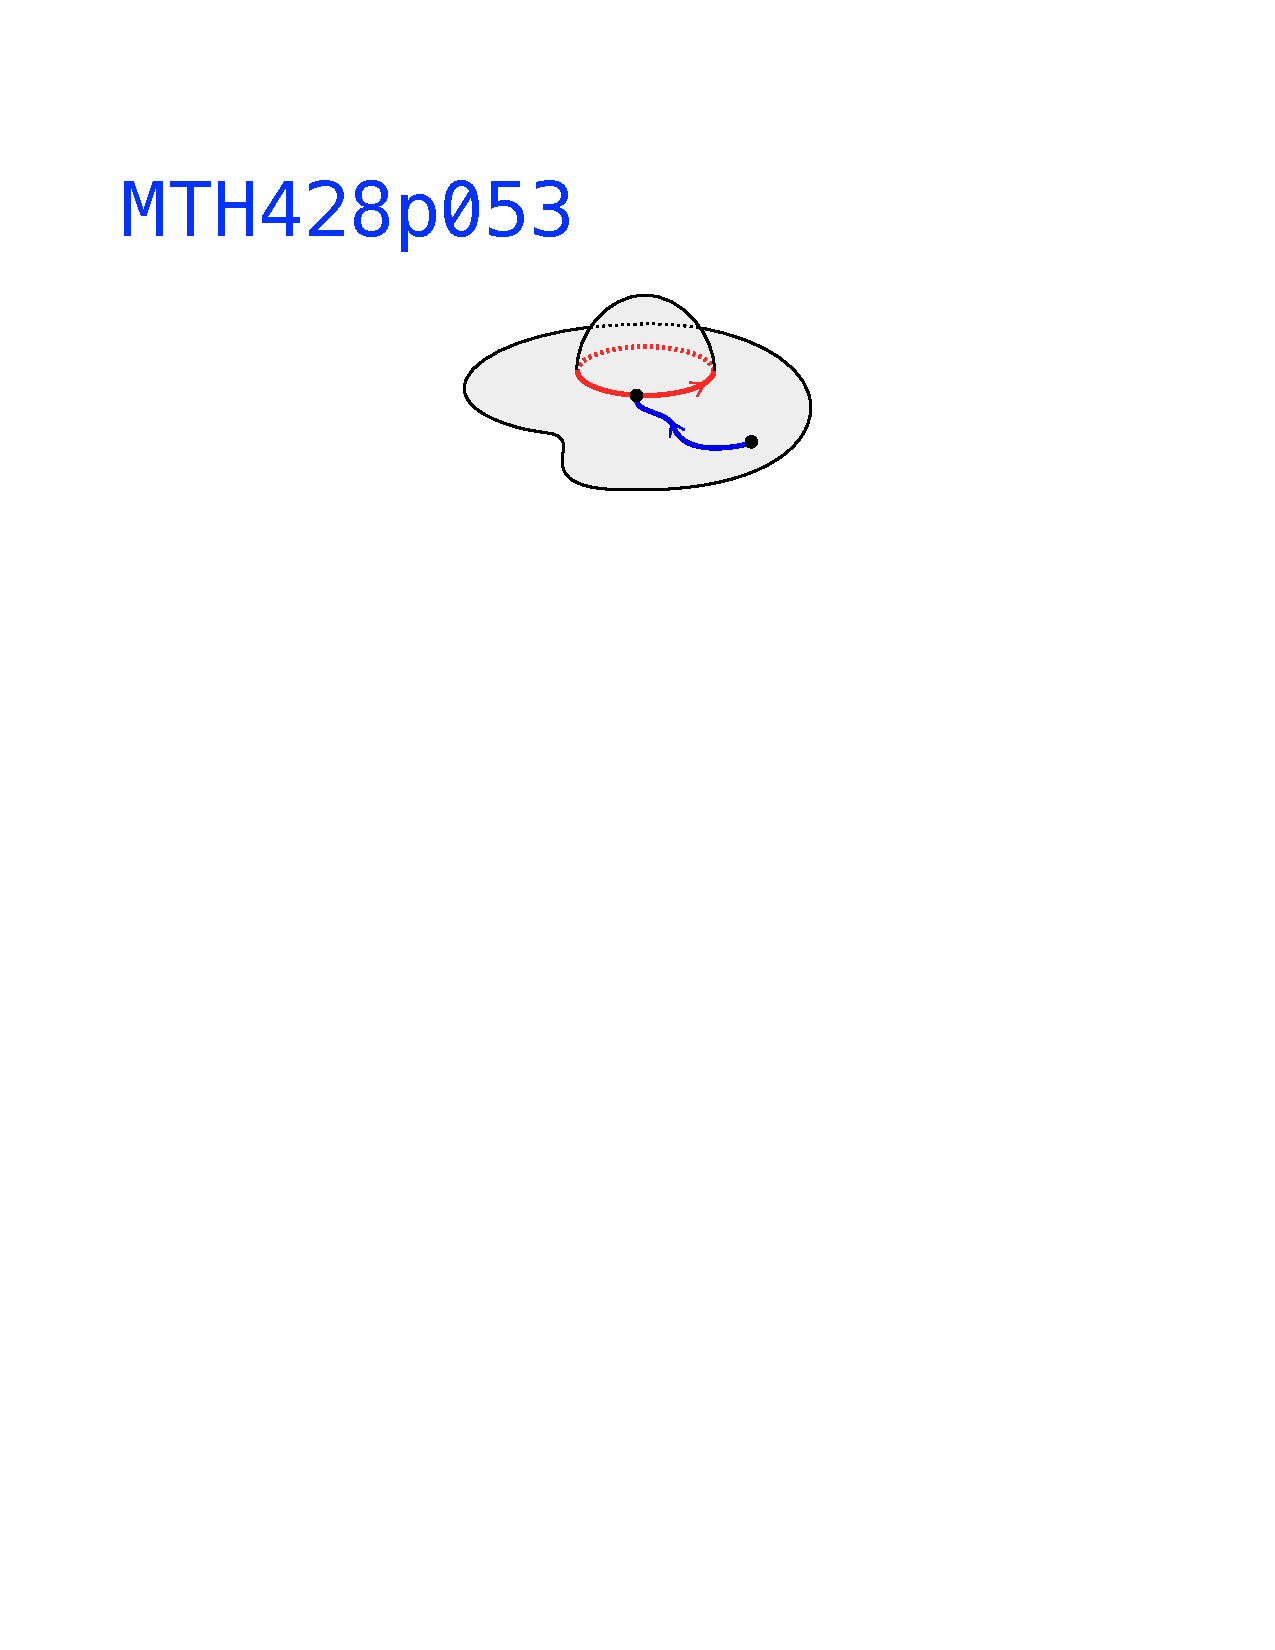
\includegraphics[width=\textwidth, trim=0mm 195mm 0mm 49mm, clip]{pictures/MTH428p053.pdf}}};

%%% COORDINATE GRID
%\draw[step=0.5, help lines] (0,0) to[grid with coordinates] (15,9);
%%% 

\node[anchor= base]  at (9.2 , 1.16){\color{red}\small  $\omega_{f}$};
\node[anchor= base]  at (8.48 , 0.78){\color{blue}\small  $\tau$};
\node[anchor= base]  at (8.4 , 2.75){ \small  $e^{2}$};
\node[anchor= base]  at (6.5 , 1.35){ \small  $Y$};
\node[anchor= base]  at (8.2 , 1.55){ \small  $f(s_{0})$};
\node[anchor= base]  at (9.8 , 0.9){\small  $x_{0}$};


\end{tikzpicture}


\end{theorem}
 %---EBLANK  # \newpage

\begin{note}
In general the element $[\tau \ast \omega_{f}\ast \xov{\tau}]\in \pi_{1}(X, x_{0})$ depends 
on the choice of the path $\tau$. However, as the statement of Theorem \ref{PI1FOR2CELLATTACH THM}
implies the  normal subgroup of $\pi_{1}(Y, x_{0})$ generated by such element does not depend on 
the choice of $\tau$. 
\end{note}


\begin{proof}[Proof of Theorem \ref{PI1FOR2CELLATTACH THM}]
Let $\xov{f}\colon D^{2} \to X$ be the characteristic map of the cell $e^{2}$
and let $y_{0}=\xov{f}((\frac{1}{2}, 0))$. Let
$U_{1} := X \ssmin \xov{f}((0, 0))$ and $U_{2} := X \ssmin Y$. The sets
$U_{1}$,  $U_{2}$, and $U_{1}\cap U_{2}$ are path connected and open in $X$. Moreover, 
$U_{1}\cup U_{2} = X$ and  $y_{0}\in U_{1}\cap U_{2}$. By van Kampen's 
Theorem we obtain
$$\pi_{1}(X, y_{0}) = \colim(\pi_{1}(U_{1}, y_{0}) \overset{i_{1\ast}}{\la} \pi_{1}(U_{1}\cap U_{2}, y_{0})
\overset{i_{2\ast}}{\ra} \pi_{1}(U_{2}, y_{0}))$$
where for $k=1, 2$ the map $i_{k}\colon U_{1}\cap U_{2} \to U_{k}$ is the inclusion. 
The space $U_{2}$ is contractible, so  $\pi_{1}(U_{2}, y_{0}) \cong \{1\}$. Also, 
$U_{1}\cap U_{2} \simeq S^{1}$, so $\pi_{1}(U_{1}\cap U_{2}, y_{0}) \cong \Z$. The generator 
of $\pi_{1}(U_{1}\cap U_{2}, y_{0})$ is represented by the loop 
$\omega'\colon [0, 1] \to U_{1}\cap U_{2}$ where 
$\omega'(s) = \bar{f}((\frac{1}{2}\cos(2\pi s), \frac{1}{2}\sin(2\pi s)))$. 
These observations show that  the homomorphism 
$j_{\ast}\colon \pi_{1}(U_{1}, y_{0})\to \pi_{1}(X, y_{0})$ induced by the 
inclusion $j\colon U_{1}\to X$ is onto, and $\ker j_{\ast}$ is the normal subgroup of $\pi_{1}(U_{1}, y_{0})$
generated  by   $[\omega'] $. 

Let $\gamma\colon [0, 1] \to X$ be the path defined by $\gamma(s) = \bar{f}(\frac{1}{2}(1+s), 0)$. 
We have $\gamma(0) = y_{0}$ and $\gamma(1) = f(s_{0})$. This path 
defines the change-of--basepoint isomorphisms $s_{\gamma} \colon \pi_{1}(X, y_{0}) \to \pi_{1}(X, f(s_{0}))$ 
and  $s_{\gamma} \colon \pi_{1}(U_{1}, y_{0}) \to \pi_{1}(U_{1}, f(s_{0}))$. 
Notice that  in $\pi_{1}(U_{1}, f(s_{0}))$ we have 
$s_{\gamma}([\omega']) = [\bar{\gamma}\ast \omega \ast \gamma] = [\omega_{f}]$:

\begin{tikzpicture}

\node[anchor=south west,inner sep=0] at (0,0) 
{{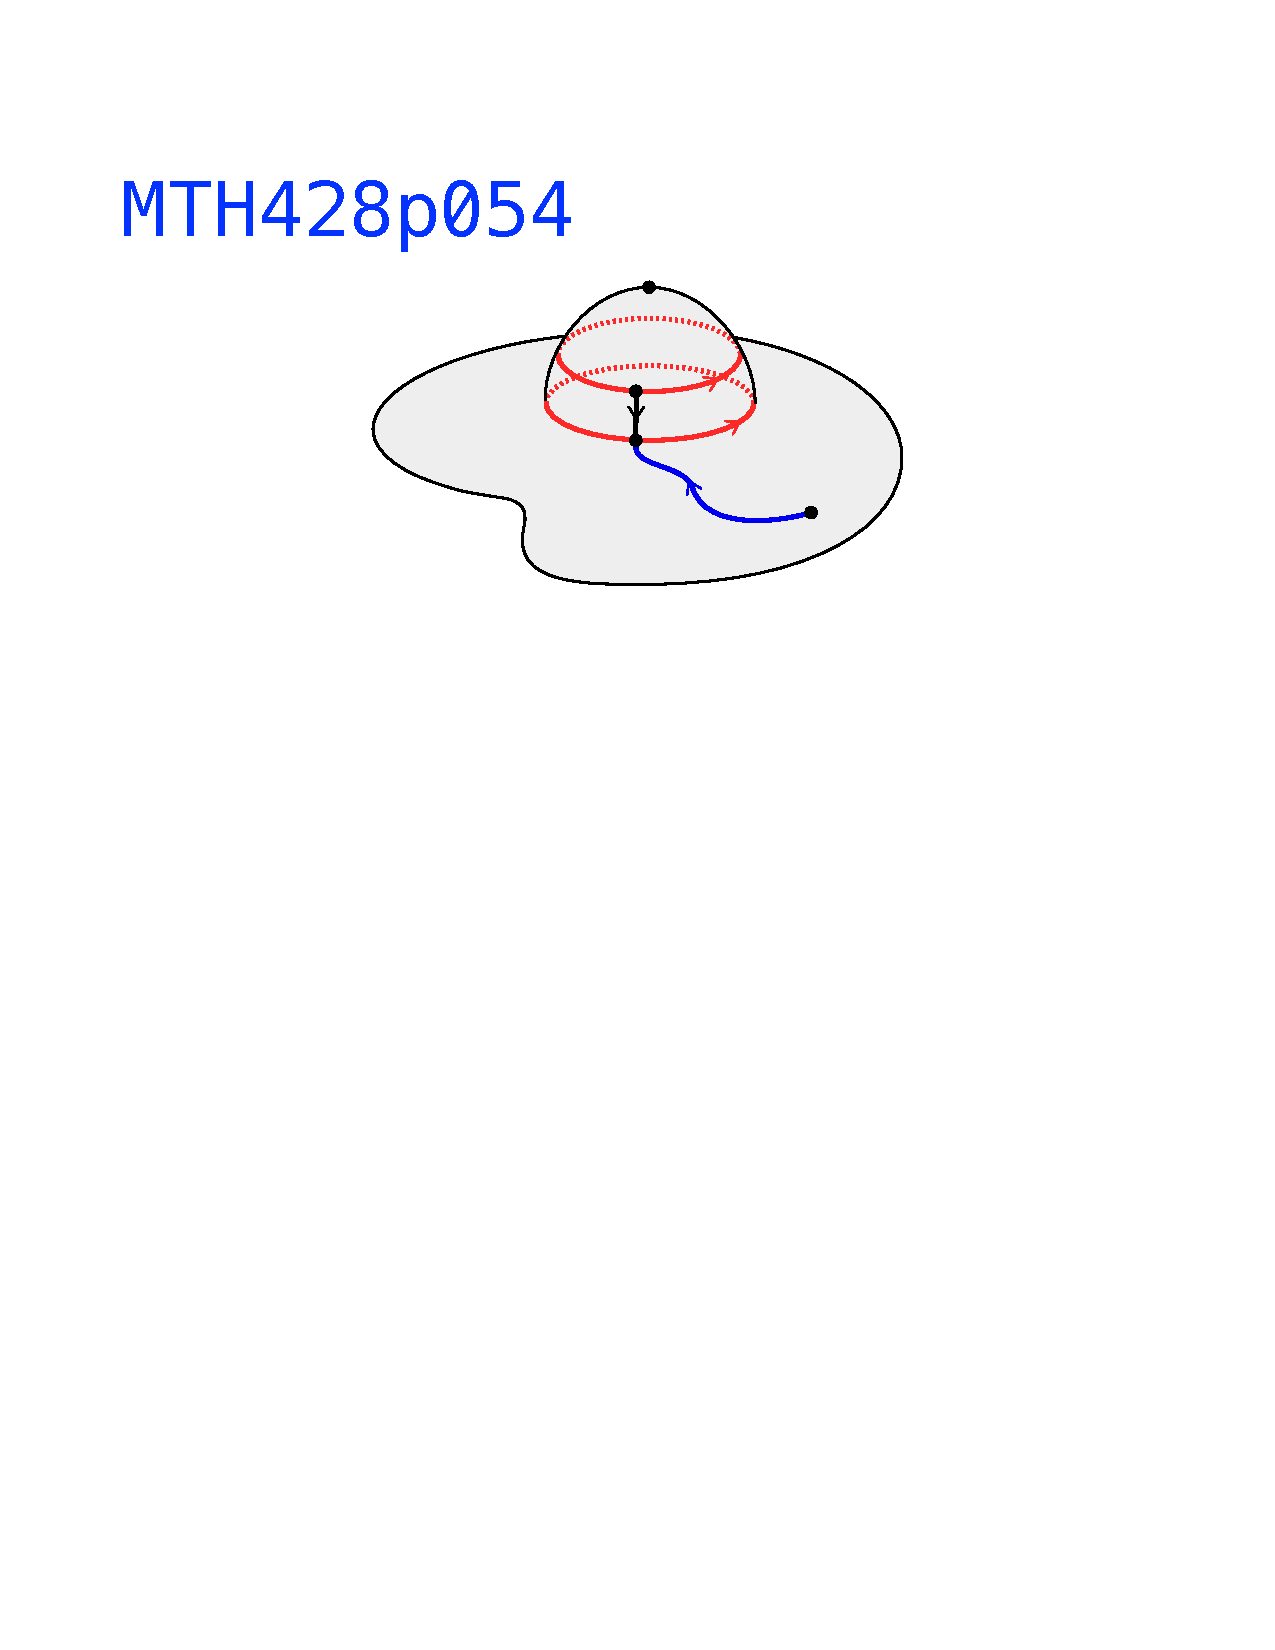
\includegraphics[width=\textwidth, trim=0mm 180mm 0mm 46mm, clip]{pictures/MTH428p054.pdf}}};

%%% COORDINATE GRID
%\draw[step=0.5, help lines] (0,0) to[grid with coordinates] (15,9);
%%% 

\node[anchor= base]  at (9.3 , 2.32){\color{red}\small  $\omega'$};
\node[anchor= base]  at (9.6 , 1.75){\color{red}\small  $\omega_{f}$};
\node[anchor= base]  at (8.5 , 2.2){ \small  $\gamma$};
\node[anchor= base]  at (8.8 , 0.95){\color{blue}\small  $\tau$};
\node[anchor= base]  at (8.37 , 4.1){ \small  $\xov{f}((0, 0))$};
\node[anchor= base]  at (7.85 , 1.55){ \small  $f(s_{0})$};
\node[anchor= base]  at (10.55 , 1.2){\small  $x_{0}$};
\fill[mygray1] (8.0, 2.75) rectangle (8.5, 3.0);
\node[anchor= base]  at (8.25 , 2.8){\small  $y_{0}$};


\end{tikzpicture}



Consider the following diagram:
\begin{equation*}
\begin{tikzpicture}[baseline=(current  bounding  box.center)]
\matrix (m) 
[matrix of math nodes, row sep=3em, column sep=2em, text height=1.5ex, text depth=0.25ex]
{
\pi_{1}(U_{1}, y_{0}) &  \pi_{1}(U_{1}, f(s_{0})) &  \pi_{1}(Y, f(s_{0})) & \pi_{1}(Y, x_{0}) \\
\pi_{1}(X, y_{0})    & \pi_{1}(X, f(s_{0}))    & \pi_{1}(X, f(s_{0}))    & \pi_{1}(X, x_{0})       \\
};
\path[->, thick, font=\scriptsize]
(m-1-1) 
edge node[anchor = east] {$j_{\ast}$} (m-2-1)
edge node[anchor = south] {$s_{\gamma}$} node[anchor= north] {$\cong$} (m-1-2)
(m-1-2) 
edge node[anchor = east] {$j_{\ast}$} (m-2-2)
(m-1-3) 
edge node[anchor = south] {$i_{\ast}$} node[anchor= north] {$\cong$} (m-1-2)
edge node[anchor = west] {$j_{\ast}$} (m-2-3)
edge node[anchor = south] {$s_{\xov{\tau}}$} node[anchor= north] {$\cong$} (m-1-4)
(m-1-4) 
edge node[anchor = west] {$j_{\ast}$} (m-2-4)
(m-2-1) 
edge node[anchor = north] {$s_{\gamma}$} node[anchor= south] {$\cong$} (m-2-2)
(m-2-3) 
edge  node[anchor = north] {$s_{\xov{\tau}}$} node[anchor= south] {$\cong$} (m-2-4)
edge node[anchor = north] {$\id$} node[anchor= south] {$\cong$} (m-2-2)
;
\end{tikzpicture}
\end{equation*}
Each square in this diagram commutes. 
The vertical homomorphisms are induced by inclusion maps. The homomorphisms  
$s_{\gamma}$ and $s_{\xov{\tau}}$ are the change-of-basepoint isomorphisms 
defined by the paths $\gamma$ and $\xov{\tau}$. The homomorphism
$i_{\ast}\colon \pi_{1}(Y, f(s_{0})) \to \pi_{1}(U_{1}, f(s_{0}))$ is induced by the 
inclusion map $Y \to U_{1}$, and it is an isomorphism since $Y$ is a deformation 
retract of $U_{1}$. Since all horizontal homomorphisms are isomorphisms 
and $j_{\ast}\colon \pi_{1}(U_{1}, d_{0}) \to \pi_{1}(X, d_{0})$ is 
onto we obtain that  $j_{\ast}\colon \pi_{1}(Y, x_{0}) \to \pi_{1}(X, x_{0})$ is also onto. Moreover, 
since the kernel of the first of these two homomorphisms is generated by 
the element $[\omega']\in \pi_{1}(U_{1}, d_{0})$ the kernel of the second is generated 
by the element 
$s_{\xov{\tau}}(i_{\ast}^{{-1}}(s_{\gamma}([\omega']))) = 
s_{\xov{\tau}}(i_{\ast}^{-1}([\omega_{f}])) = s_{\xov{\tau}}([\omega_{f}]) = 
[\tau\ast \omega_{f} \ast \xov{\tau}]$.

\end{proof}

Theorem \ref{PI1FOR2CELLATTACH THM} can be generalized to the case when we are attaching 
an arbitrary (finite or infinite) number of $2$-cells. In the statement below we use the same notation as in 
Theorem \ref{PI1FOR2CELLATTACH THM}:  if $f$ is an attaching map of a $2$-cell then by $\omega_{f}$
we denote the loop defined by $f$ and by $f(s_{0})$ the starting/ending point of this loop. 


 %---BBLANK 
\begin{theorem}
\label{PI1OF2DIMCW THM}
Let  $Y$ be a path connected space with basepoint $x_{0}\in Y$
and let $X$ be a space obtained by attaching to $Y$ a 
collection of $2$-cells:  $X = Y\cup\{e^{2}_{i}\}_{i\in I}$. Let $f_{i}\colon S^{1}\to X$ be the attaching map 
of the cell $e^{2}_{i}$ and let $\tau_{i}\colon [0, 1] \to Y$ be a path such that 
$\tau_{i}(0) = x_{0}$ and $\tau_{i}(1) = f_{i}(s_{0})$. 
 The homomorphism 
$$j_{\ast}\colon \pi_{1}(Y, x_{0}) \to \pi_{1}(X, x_{0})$$
induced by the inclusion map $j\colon Y \to X$ is onto, and so 
$\pi_{1}(X, x_{0}) \cong \pi_{1}(Y, y_{0})/\Ker(j_{\ast})$. Moreover, $\Ker(j_{\ast})$ is the normal subgroup 
of $\pi_{1}(Y, x_{0})$  generated by set  $\{[\tau_{i} \ast \omega_{f_{i}}\ast \xov{\tau_{i}}]\}_{i\in I}$. 
\end{theorem}
 %---EBLANK  # \newpage



 %---BBLANK 
\begin{example}
 %---EBLANK  # Torus
Recall that the torus $T$ has a CW-complex structure with one 0-cell, two 1-cells and one 2-cell:
 
  %---BBLANK 
 \begin{tikzpicture}

\node[anchor=south west,inner sep=0] at (0,0) 
{{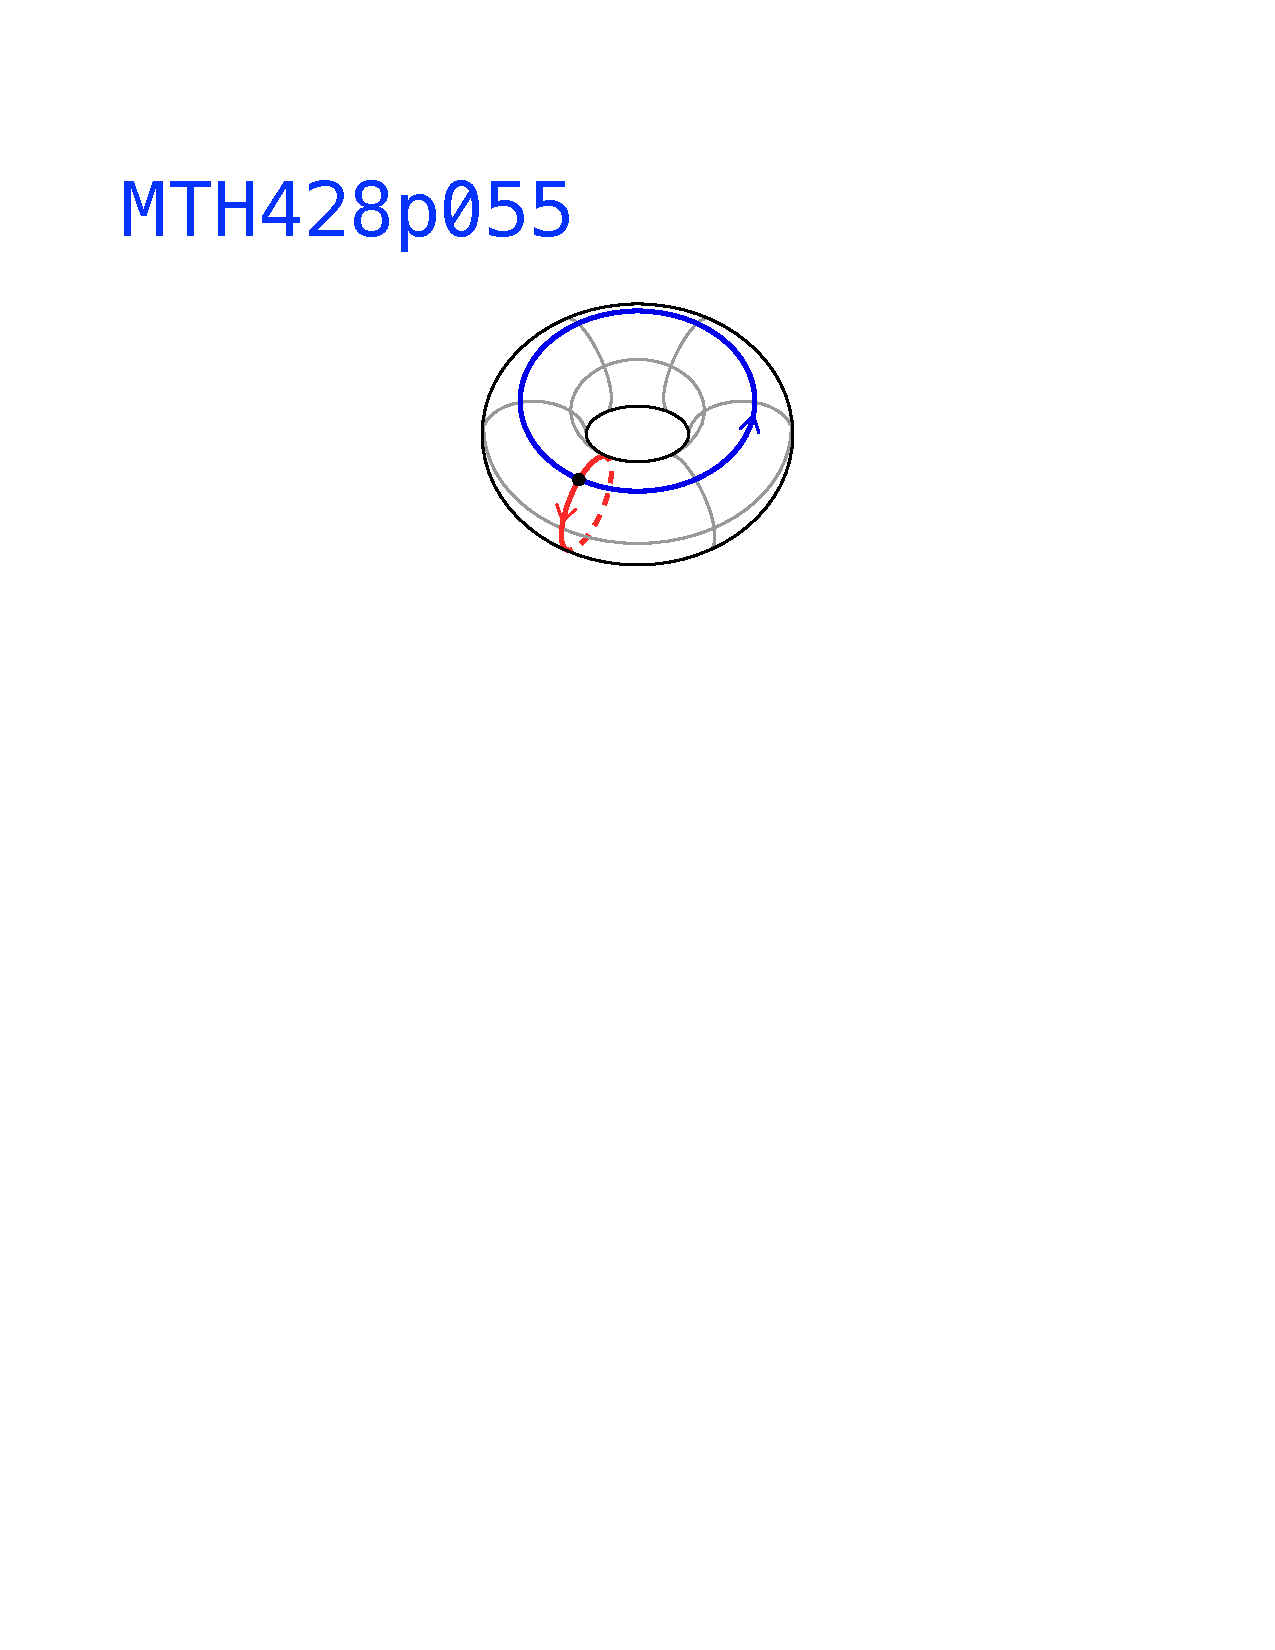
\includegraphics[width=\textwidth, trim=0mm 183mm 0mm 50mm, clip]{pictures/MTH428p055.pdf}}};

%%% COORDINATE GRID
%\draw[step=0.5, help lines] (0,0) to[grid with coordinates] (15,9);
%%% 
\node[anchor= base]  at (7.43 , 1.4){\small  $x_{0}$};
\end{tikzpicture}
 %---EBLANK # \end{example} \newpage


We will take the $0$-cell $x_{0}$ as the basepoint of $T$.  
The $1$-skeleton $T^{(1)}$ of the torus is homeomorphic to $S^{1}\vee S^{1}$, so 
$\pi_{1}(T^{(1)}, x_{0})\cong \Z\ast \Z$. Denote by $a$ the element of 
 $\pi_{1}(T^{(1)}, x_{0})$ represented by the loop that goes once around one $1$-cell 
 and by $b$ the element  represented by the loop that goes once around the second $1$-cell. 
The elements $a, b$ freely generate the group $\pi_{1}(T^{(1)}, x_{0})$, i.e.  we have 
an isomorphism $\pi_{1}(T^{(1)}, x_{0}) \cong \langle a, b\rangle$. Let 
 $f\colon S^{1} \to T^{(1)}$ be the attaching map of the $2$-cell.  The loop $\omega_{f}$
 represents the element $aba^{-1}b^{-1} \in \pi_{1}(T^{(1)}, x_{0})$:
 
 
 \begin{tikzpicture}

\node[anchor=south west,inner sep=0] at (0,0) 
{{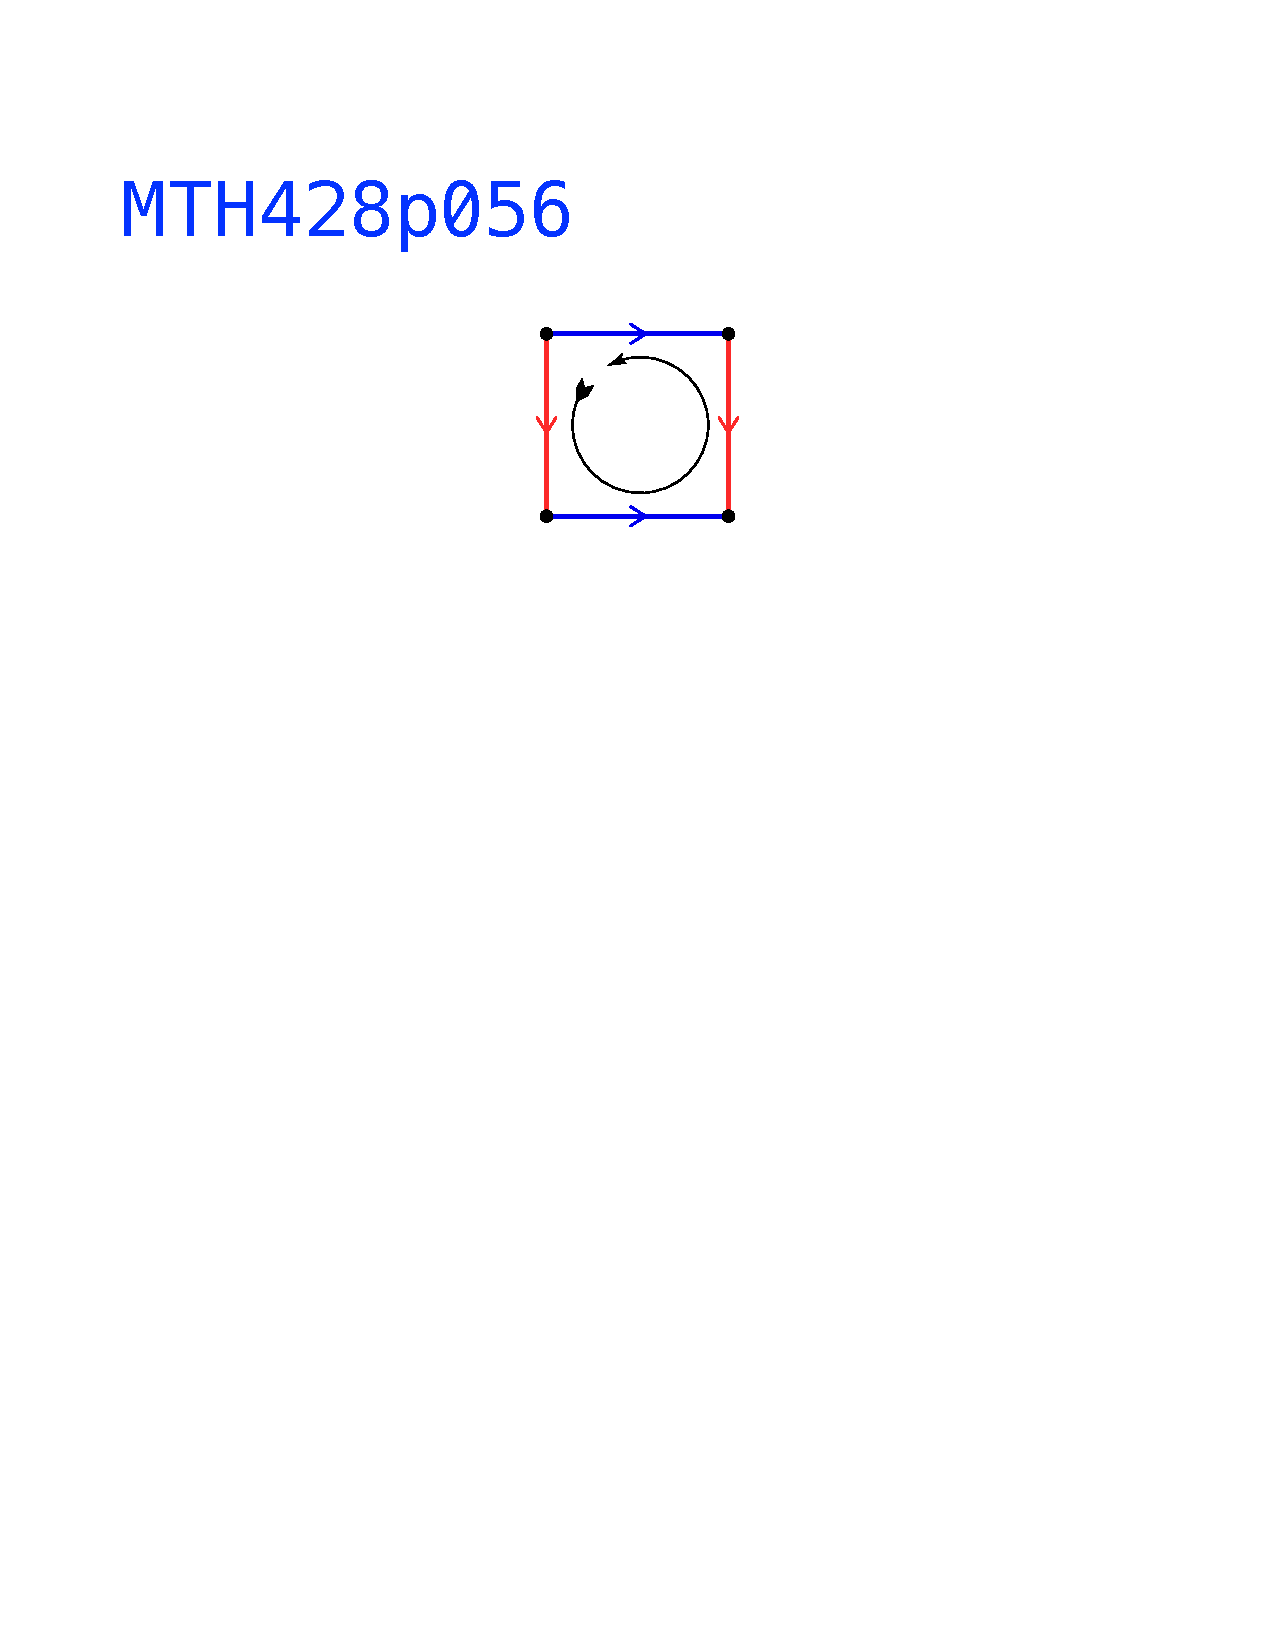
\includegraphics[width=\textwidth, trim=0mm 189mm 0mm 54mm, clip]{pictures/MTH428p056.pdf}}};

%%% COORDINATE GRID
%\draw[step=0.5, help lines] (0,0) to[grid with coordinates] (15,9);
%%% 
\node[anchor= base]  at (8.3 , 1.35){\small  $\omega_{f}$};
\node[anchor= base]  at (8.3 , 2.83){\small \color{blue} $b$};
\node[anchor= base]  at (8.3 , -0.15){\small \color{blue} $b$};
\node[anchor= base]  at (6.8 , 1.35){\small \color{red} $a$};
\node[anchor= base]  at (9.75 , 1.35){\small \color{red} $a$};
\end{tikzpicture}
 
 By Theorem  \ref{PI1FOR2CELLATTACH THM} we get  
 $\pi_{1}(T, x_{0}) \cong \langle a, b \rangle/N$ where $N$ is the normal subgroup 
 of $\langle a, b\rangle$ generated by the element $aba^{-1}b^{-1}$. In other words 
 we obtain a presentation of $\pi_{1}(T, x_{0})$:
 $$\pi_{1}(T, x_{0}) \cong \langle a, b \ | \  aba^{-1}b^{-1} \rangle $$ 
 Since $\langle a, b \ | \  aba^{-1}b^{-1} \rangle  \cong \Z\times \Z$ we recover the result 
we obtained before  (\ref{PI1TORUS EXAMPLE}) using the product formula for the fundamental group.


\end{example}

 %---BBLANK 
\begin{example} 
 %---EBLANK  # Klein bottle
Recall the CW-complex structure on the Klein bottle K:

  %---BBLANK 
 \begin{tikzpicture}

\node[anchor=south west,inner sep=0] at (0,0) 
{{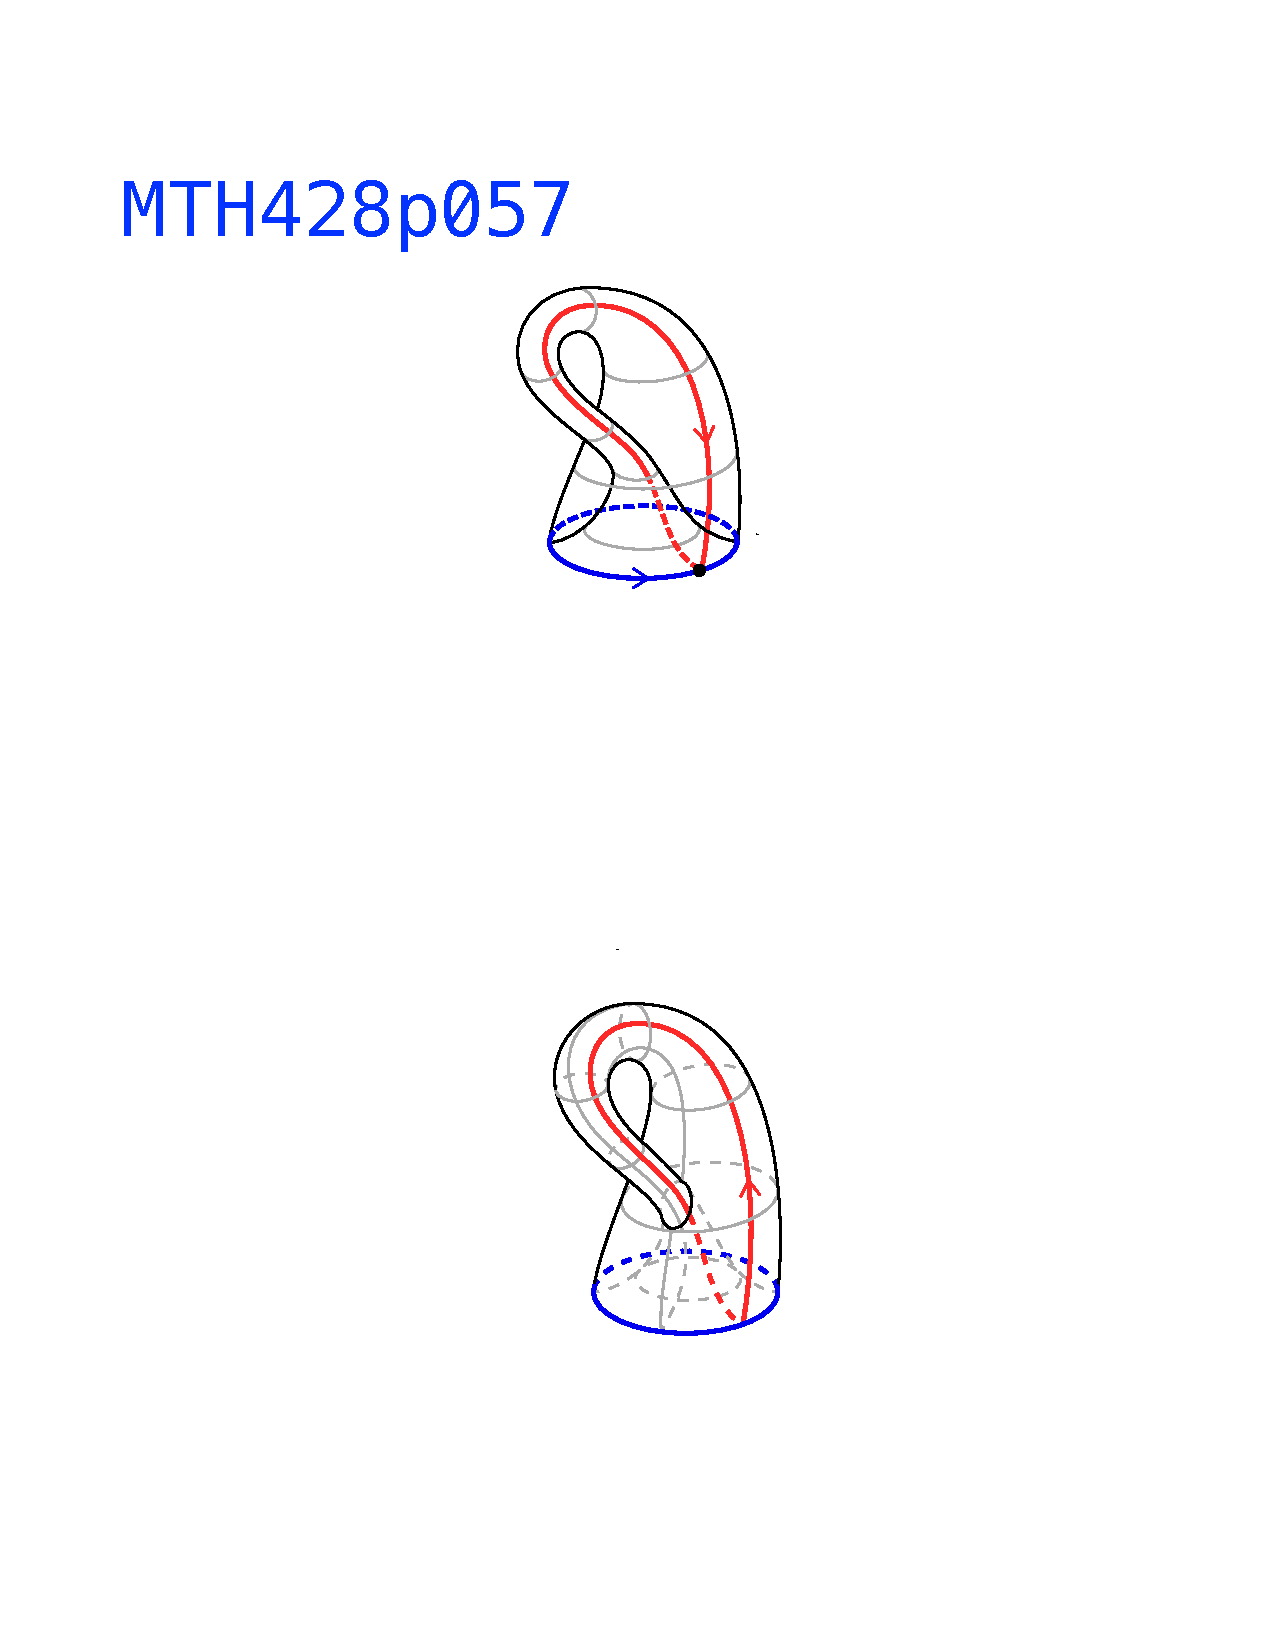
\includegraphics[width=\textwidth, trim=0mm 178mm 0mm 47mm, clip]{pictures/MTH428p057.pdf}}};

%%% COORDINATE GRID
%\draw[step=0.5, help lines] (0,0) to[grid with coordinates] (15,9);
%%% 
\node[anchor= base]  at (9.2 , 0.1){\small  $x_{0}$};
\end{tikzpicture}
 %---EBLANK  # \end{example} \newpage

Again, we will take the  $0$-cell in this complex as the basepoint.  
The $1$-skeleton $K^{(1)}$ is homeomorphic to $S^{1}\vee S^{1}$, so 
$\pi_{1}(K^{(1)}, x_{0}) \cong \langle a, b \rangle$ where $a, b$ are represented by the loops 
traversing each of the $1$-cells. The attaching map of the $2$-cell represents the element 
$aba^{-1}b\in \langle a, b \rangle$:

 \begin{tikzpicture}

\node[anchor=south west,inner sep=0] at (0,0) 
{{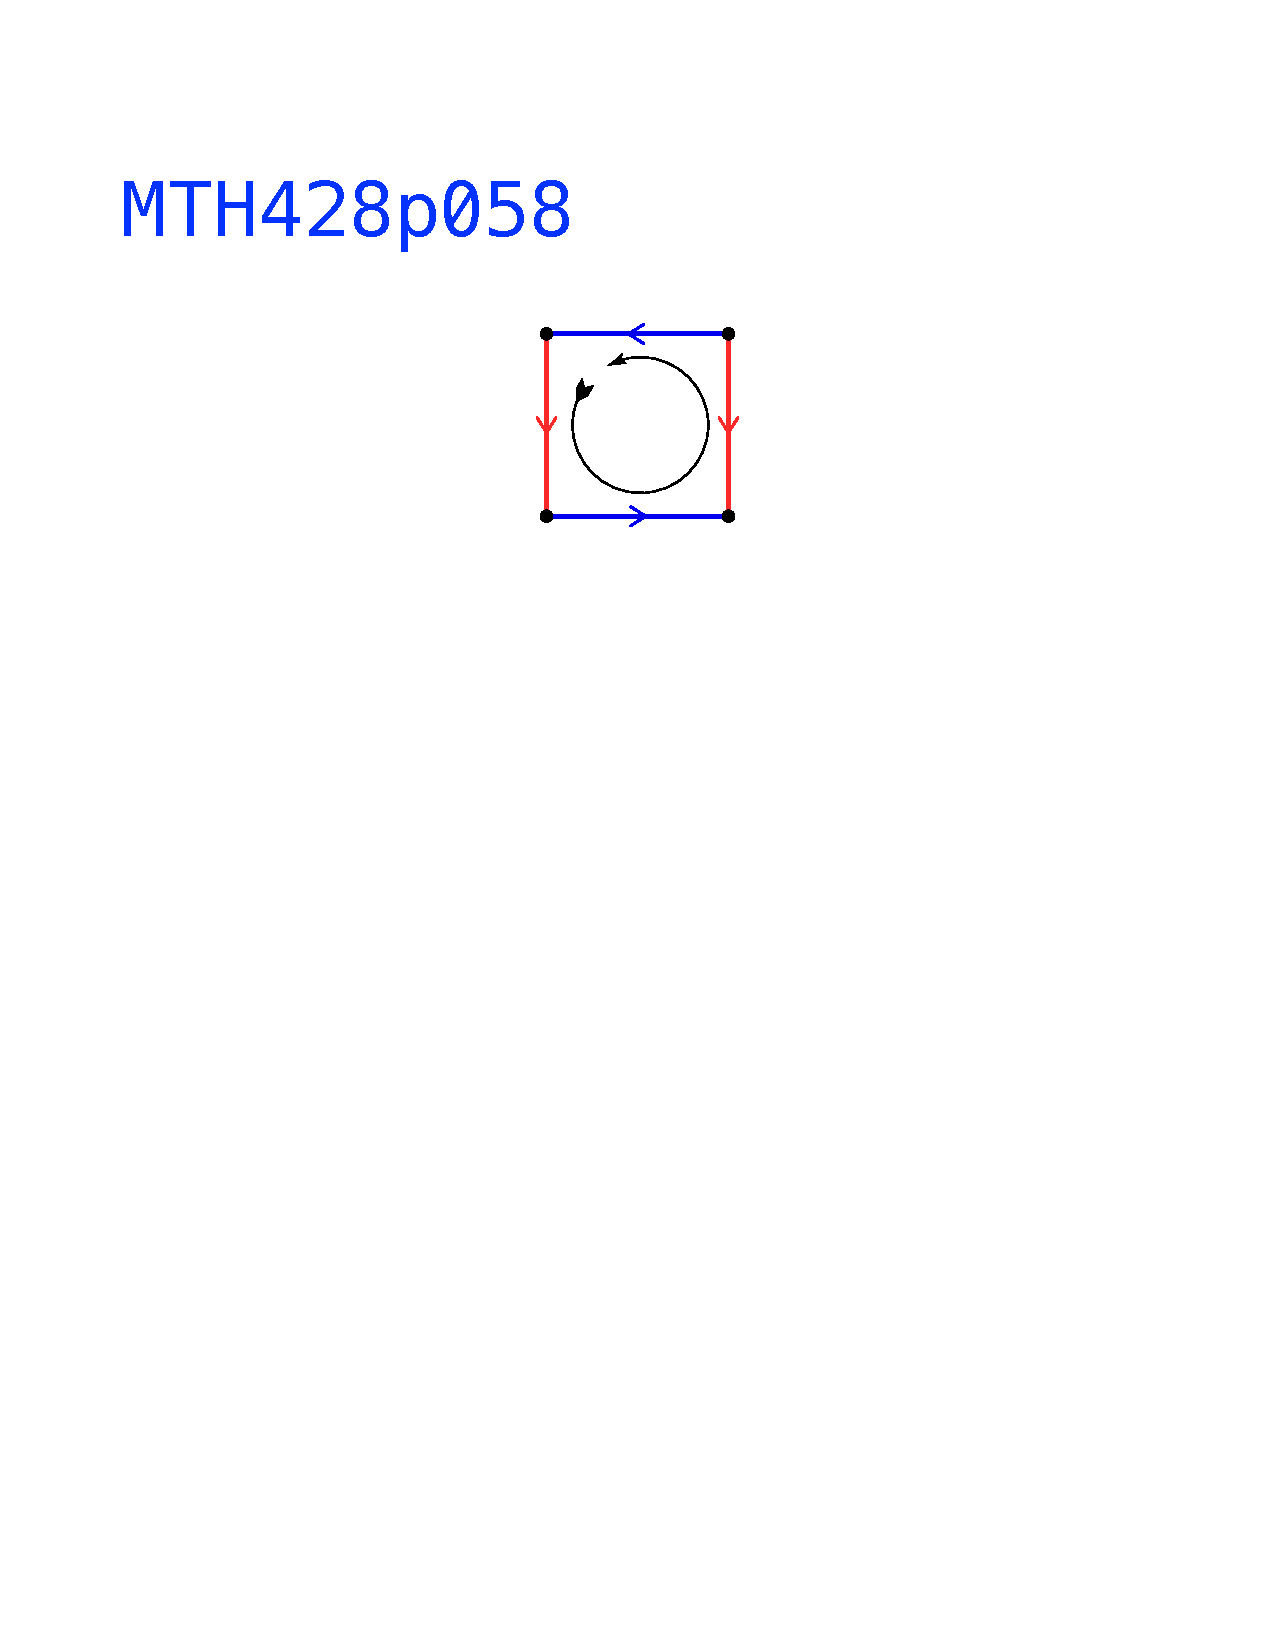
\includegraphics[width=\textwidth, trim=0mm 189mm 0mm 54mm, clip]{pictures/MTH428p058.pdf}}};

%%% COORDINATE GRID
%\draw[step=0.5, help lines] (0,0) to[grid with coordinates] (15,9);
%%% 
\node[anchor= base]  at (8.3 , 1.35){\small  $\omega_{f}$};
\node[anchor= base]  at (8.3 , 2.83){\small \color{blue} $b$};
\node[anchor= base]  at (8.3 , -0.15){\small \color{blue} $b$};
\node[anchor= base]  at (6.8 , 1.35){\small \color{red} $a$};
\node[anchor= base]  at (9.75 , 1.35){\small \color{red} $a$};
\end{tikzpicture}

It follows that $\pi_{1}(K, x_{0}) \cong \langle a, b \ | \ aba^{-1}b \rangle$. 

\end{example}

 %---BBLANK 
\begin{example}
 %---EBLANK  #  $\RP^{2}$ 
Recall that $2$-dimensional projective space $\RP^{2}$ has a cell structure with one $0$-cell, 
one $1$-cell and one  2-cell:

 %---BBLANK 
\begin{tikzpicture}

\node[anchor=south west,inner sep=0] at (0,0) 
{{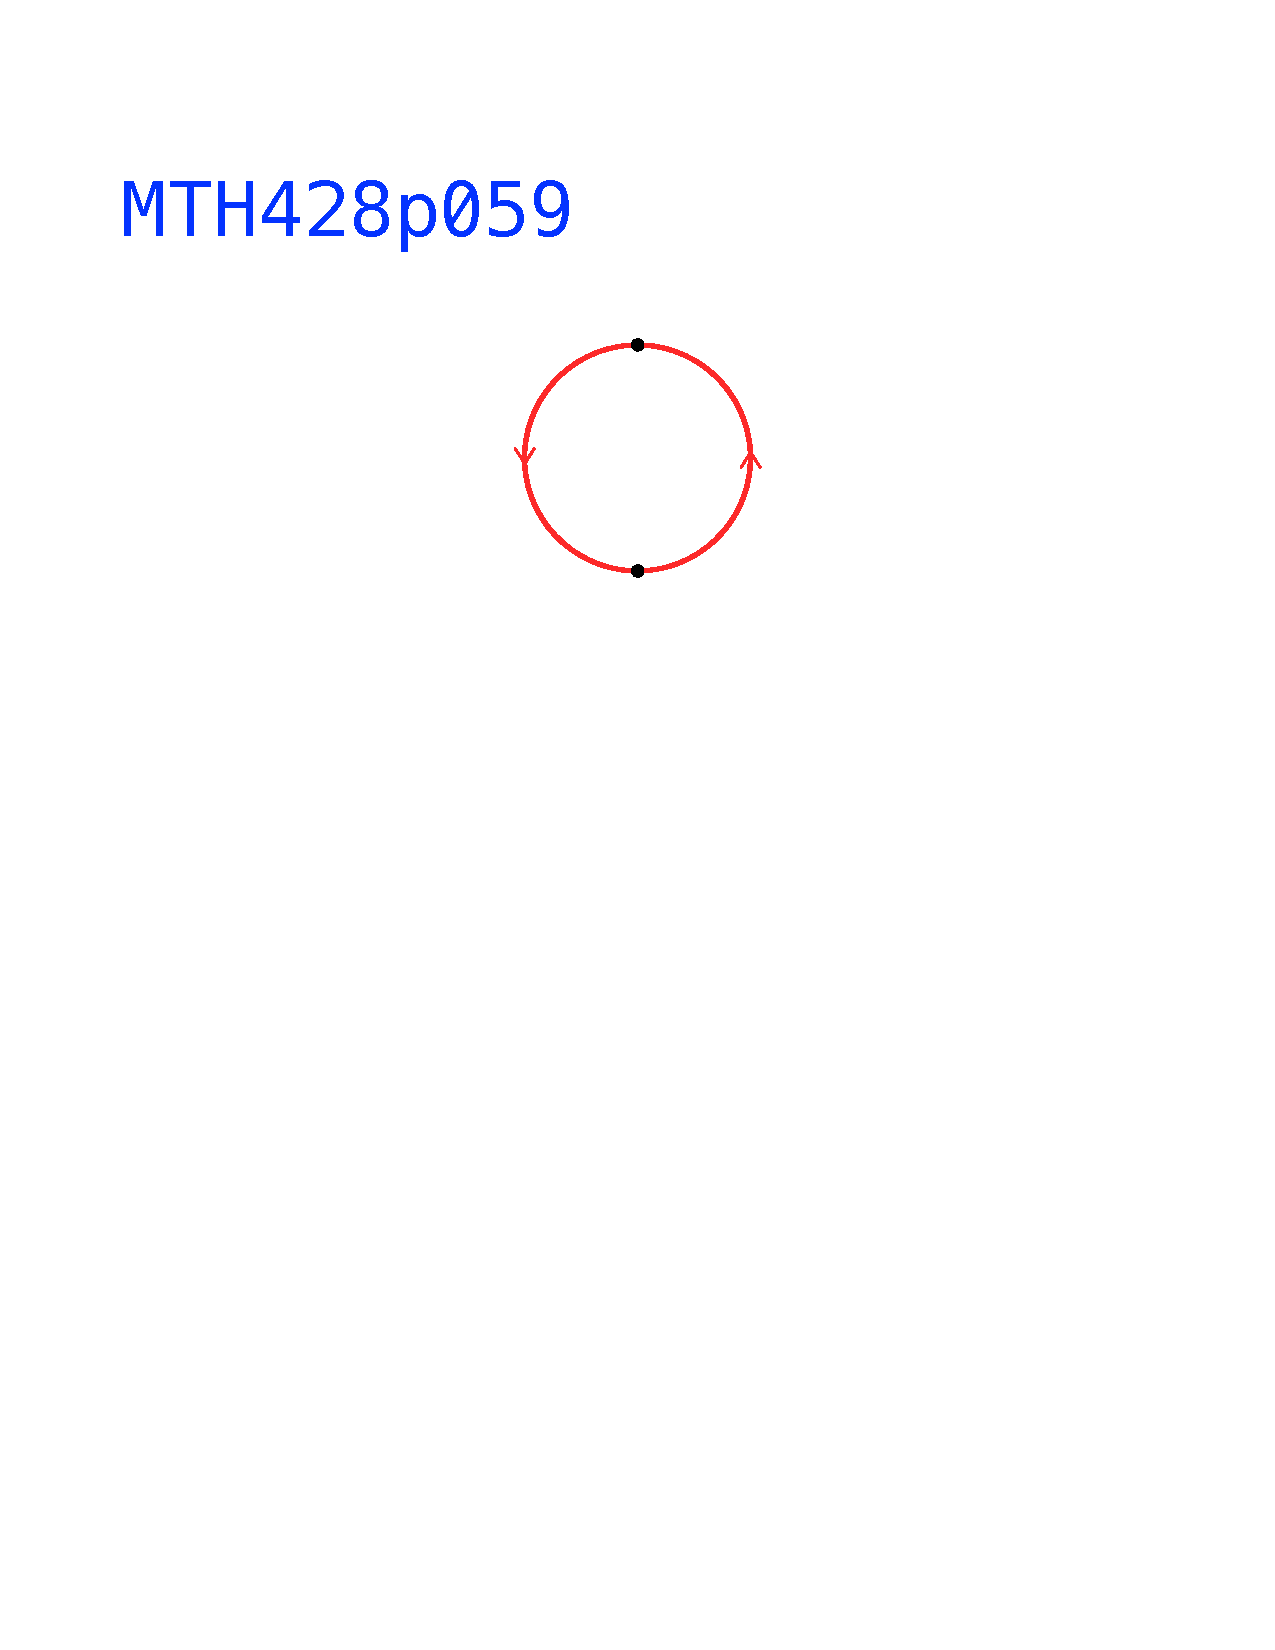
\includegraphics[width=\textwidth, trim=0mm 181mm 0mm 55mm, clip]{pictures/MTH428p059.pdf}}};

%%% COORDINATE GRID
%\draw[step=0.5, help lines] (0,0) to[grid with coordinates] (15,9);
%%% 
\node[anchor= base]  at (8.32 , 3.25){\small  $e^{0}$};
\node[anchor= base]  at (8.32 , -0.32){\small  $e^{0}$};
\node[anchor= base east]  at (6.75 , 1.57){\color{red} \small  $e^{1}$};
\node[anchor= base west]  at (9.8 , 1.57){\color{red} \small  $e^{1}$};
\node[anchor= base ]  at (8.32 , 1.57){\small  $e^{2}$};
\end{tikzpicture}
 %---EBLANK  #  \end{example} \newpage

We will take the $0$-cell as the basepoint $x_{0}\in \RP^{2}$.
The one skeleton  $(\RP^{2})^{(1)}$ is homeomorphic to $S^{1}$, so
$\pi_{1}((\RP^{2})^{(1)}, x_{0}) \cong \langle a \rangle $
where $a$ denotes the generator represented by the loop that traverses the $1$-cell. 
The attaching map $f\colon S^{1} \to (\RP^{2})^{(1)}$ for the $2$-cell corresponds to the element $a^{2}$:

\begin{tikzpicture}

\node[anchor=south west,inner sep=0] at (0,0) 
{{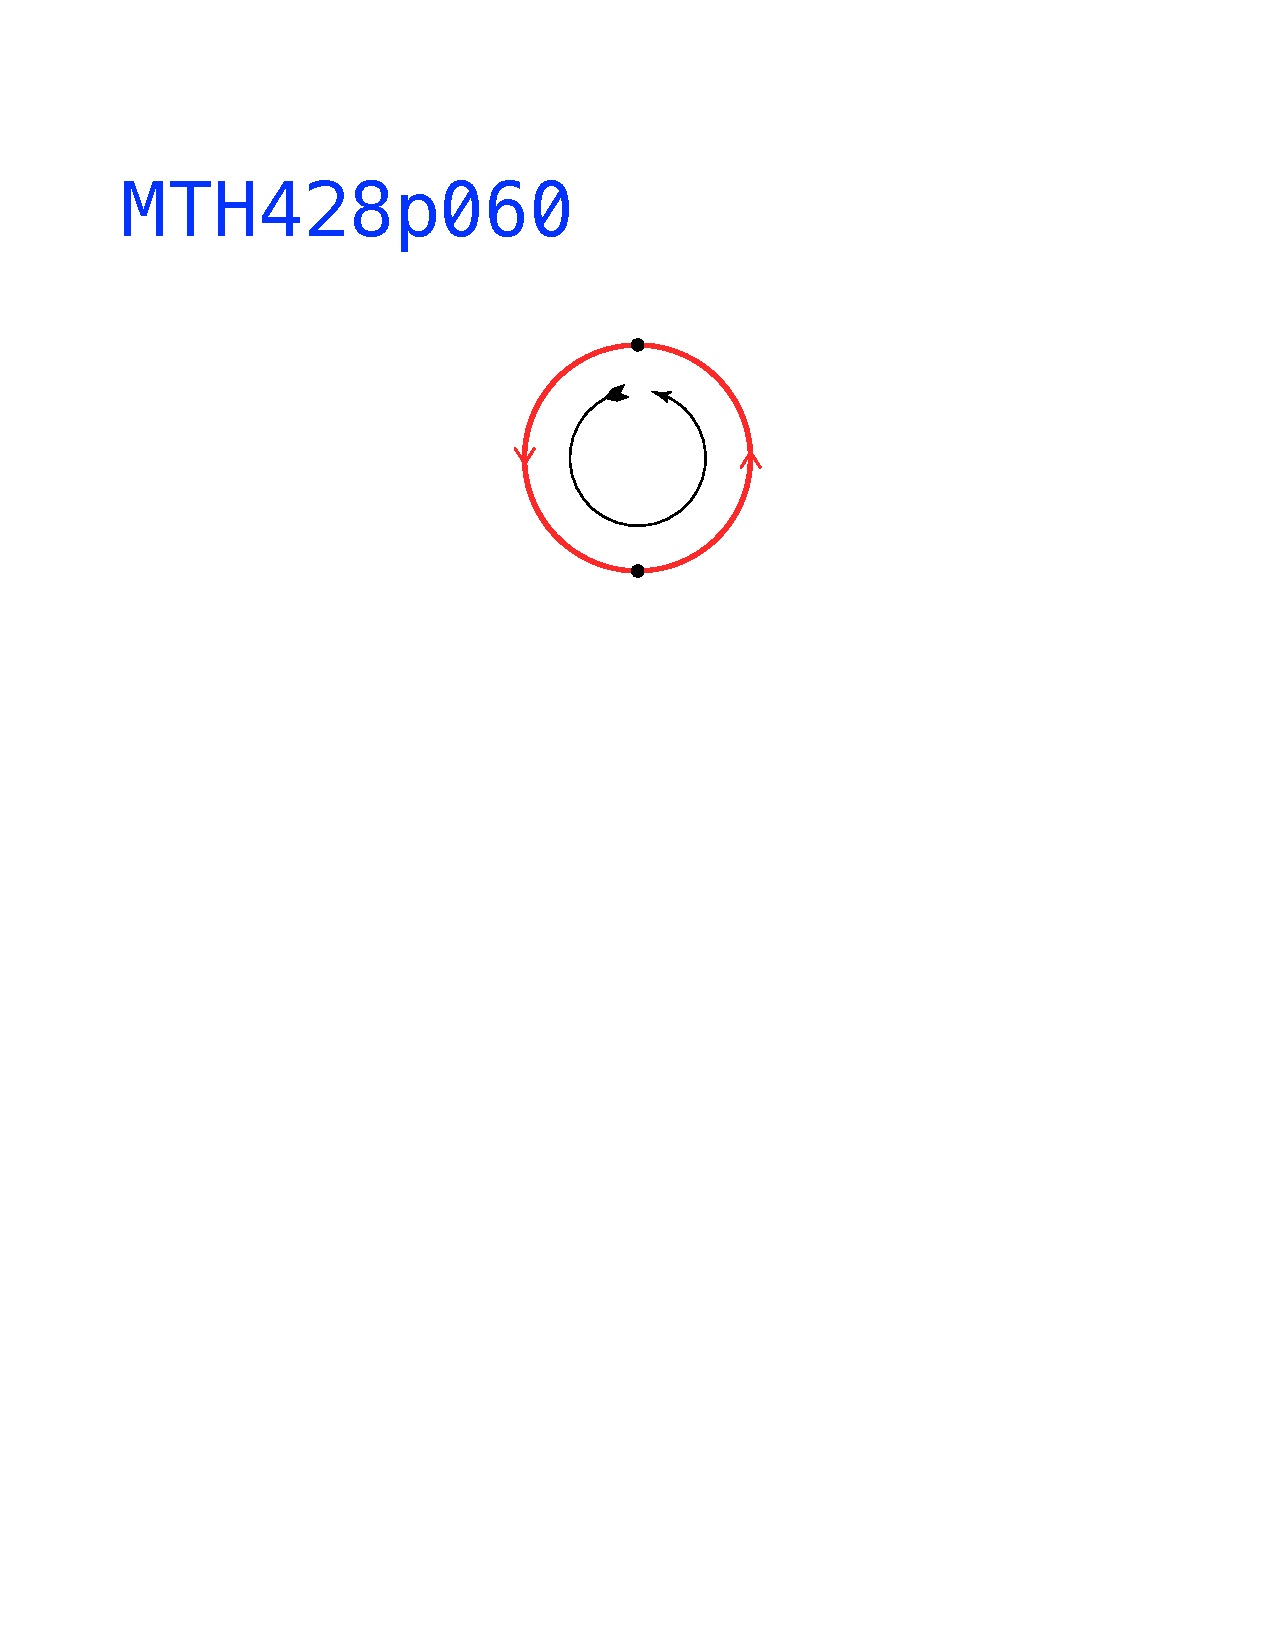
\includegraphics[width=\textwidth, trim=0mm 181mm 0mm 55mm, clip]{pictures/MTH428p060.pdf}}};

%%% COORDINATE GRID
%\draw[step=0.5, help lines] (0,0) to[grid with coordinates] (15,9);
%%% 
\node[anchor= base]  at (8.32 , 3.25){\small  $x_{0}$};
\node[anchor= base]  at (8.32 , -0.32){\small  $x_{0}$};
\node[anchor= base east]  at (6.75 , 1.57){\color{red} \small  $a$};
\node[anchor= base west]  at (9.8 , 1.57){\color{red} \small  $a$};
\node[anchor= base ]  at (8.32 , 1.57){\small  $\omega_{f}$};
\end{tikzpicture}


As a consequence $\pi_{1}(\RP^{2}, x_{0}) \cong \langle a \ | \ a^{2} \rangle \cong \Z/2$. 

\end{example}


 %---BBLANK  
\begin{note}
 %---EBLANK  # Abelianization. \end{note} \newpage
The computations above show right away that the torus $T$ is not homotopy equivalent to $\RP^{2}$
since $\pi_{1}(T) \cong \Z\oplus \Z \not\cong \Z/2\Z \cong \pi_{1}(\RP^{2})$.  It may be less clear  though
whether the fundamental group of the Klein bottle is isomorphic or not to one of these groups. We can resolve 
this problems as follows. If $G$  is a group and $g, h\in G$ then the \emph{commutator} 
of $g$ and $h$ is the element $[g, h] = ghg^{-1}h^{-1}$. Notice that $[g, h]$ is the trivial element 
if and only if $gh= hg$. The \emph{commutator subgroup} of $G$
is the subgroup $[G, G]$ generated by the set $\{[g, h] \ | \ g, h\in G\}$. Since  $[G, G]$ is a normal 
subgroup of $G$ (exercise) we can consider the quotient group $G_{ab} = G/[G, G]$ which is 
called the \emph{abelianization} of $G$. The construction of $G_{ab}$ has the following properties (exercise):
\benu
\item[\textbullet] $G_{ab}$ is an abelian group.
\item[\textbullet] If $G$ is an abelian then $G_{ab}\cong G$. 
\item[\textbullet] If $f\colon G \to H$ is a group homomorphism then $f([G, G])\subseteq [H, H]$, and so 
$f$ induces a homomorphism $f_{ab}\colon G_{ab} \to H_{ab}$. 
\item[\textbullet] Recall that $\Gr$ denotes the category of all groups. Denote by $\Ab$ the category 
of abelian groups whose elements are all abelian groups and morphisms are homomorphisms of 
such groups. The assignments $F(G) = G_{ab}$ and $F(f) = f_{ab}$ define a functor 
$$F\colon \Gr\to \Ab$$
This implies in particular that if  $G\cong G'$ then $G_{ab}\cong G'_{ab}$. 

\eenu
 
Since the groups $\pi_{1}(T)$ and $\pi_{1}(\RP^{2})$ are abelian we have 
$\pi_{1}(T)_{ab} \cong \pi_{1}(T)$ and $\pi_{1}(\RP^{2})_{ab}\cong \pi_{1}(\RP^{2})$. On the other hand 
abelianization of the fundamental group of the Klein bottle $\pi_{1}(K)\cong \langle a, b \ | aba^{-1}b\rangle$
is obtained by imposing the  condition that $ab=ba$, or equivalently adding the relation 
$aba^{-1}b^{-1}$ to the presentation of the group:
$$\pi_{1}(K)_{ab}\cong \langle a, b \ | \ aba^{-1}b, \ aba^{-1}b^{-1}\rangle$$
Notice that if $ab = ba$ then $aba^{-1}b = b^{2}$. Therefore  we obtain:
$$\pi_{1}(K)_{ab}\cong \langle a, b \ | \ b^{2}, \ aba^{-1}b^{-1}\rangle \cong \Z\oplus \Z/2\Z$$ 
Since $\pi_{1}(K)_{ab}$ is isomorphic to neither $\pi_{1}(T)_{ab}$ nor $\pi_{1}(\RP^{2})_{ab}$
we get that  the $K\not\simeq T$ and $K\not \simeq \RP^{2}$.  
\end{note}

As the final result of this chapter we will show that any group can be realized as the fundamental group 
of some CW-complex:


 %---BBLANK  
\begin{theorem}
\label{REALIZINGGPBYP1X THM}
For any group $G$ there exists a CW-complex $X$ such that $\pi_{1}(X)\cong G$. 
\end{theorem}
 %---EBLANK  # \newpage

\begin{proof}
We will construct the complex $X$ as follows. The $0$-skeleton of $X$ consists of a single 
$0$-cell that we will take as the basepoint $x_{0}$. The  $1$-skeleton of $X$ is the wedge 
of circles, one copy of $S^{1}$ for each element of $G$: 
$$X^{(1)} = \bigvee_{g\in G} S^{1}$$
Let $\omega_{g}$ denote the loop in $X^{(1)}$ that traverses the copy of $S^{1}$ corresponding 
the element $g\in G$. The group $\pi_{1}(X^{(1)}, x_{0})$ is the free group generated by the 
set  $T = \{[\omega_{g}] \in \pi_{1}(X^{(1)}, x_{0} \ | \ g\in G \}$.  Consider the function of sets 
$f\colon T\to G$ given by $f([\omega_{g}]) = g$. By the universal property of free groups 
(\ref{UNIVPROPFREEGPS THM}) this function defines  a homomorphims of groups
$\xov{f}\colon \pi_{1}(X^{(1)}, x_{0}) \to G$. Moreover, since $f$ is onto thus so is $\xov{f}$. 
As a consequence we obtain that $G\cong \pi_{1}(X^{(1)}, x_{0})/\Ker(\xov{f})$. For each 
element $r\in \Ker(\xov{f})$ let $\sigma_{r}\colon [0, 1] \to X^{(1)}$ be a loop representing $r$. 
Recall (\ref{PI1THROUGHS1 NOTE}) that such loop can be identified with a map $S^{1}\to X^{(1)}$. 
By abuse of notation we will denote this map also by $\sigma_{r}$. Let $X$ be the CW-complex 
obtained from $X^{(1)}$ by attaching one $2$-cell for each element $r\in \Ker(\xov{f})$ with the 
attaching map given by $\sigma_{r}$. By Theorem \ref{PI1OF2DIMCW THM} we obtain 
$$\pi_{1}(X, x_{0})\cong \pi_{1}(X^{(1)}, x_{0})/\Ker{(\xov{f})} \cong G$$
\end{proof}


\begin{note}
By modifying the proof Theorem \ref{REALIZINGGPBYP1X THM} we can show that 
if a group $G$ has a presentation $G\cong \langle S \ | \ R \rangle$ then $G$ is isomorphic 
to the fundamental group of a CW-complex $X$ which has one $1$-cell for each element of 
$S$ and one $2$-cell for each element of $R$. In particular $G$ is finitely generated if and only if 
$G\cong \pi_{1}(X)$ for some $CW$-complex $X$ such that $X^{(1)}$ is finite, and and 
$G$ is finitely presented if and only if $G\cong \pi_{1}(X)$ for some finite CW-complex $X$.  
\end{note}


%%%%%%%%%%%%%%%%%%%%%%%%%%%%%%%
%  EXERCISES
%%%%%%%%%%%%%%%%%%%%%%%%%%%%%%%

\exercises

\begin{exercise}
Let $x_{1}, x_{2}, x_{3} \in S^{2}$ and let $X$ be the quotient space obtained by identifying 
these three points. Put a CW-complex structure on $X$ and use it to compute $\pi_{1}(X)$. 
\end{exercise}

\begin{exercise}
Let $T$ be the torus. The \emph{connected sum} $T\# T$ is the space obtained as follows. 
Take $D\subseteq T$ to be a subspace homeomorphic to the closed disk $D^{2}$ and let $\text{Int}(D)$, 
$\text{Bd}(D)$ denote, respectively, the interior and the boundary of $D$. The space $\text{Int}(D)$
is homeomorphic to the open disc and $\text{Bd}(D)$ to the circle $S^{1}$. Take the space 
$\{0, 1\}$ with the discrete topology. We set:
$$T\# T = (T\setminus D) \times \{0, 1\}/{\sim}$$
where $(x, 0)\sim (x, 1)$ for each $x\in \text{Bd}(D)$. In other words $T\# T$ is obtained by taking two copies 
of the torus, cutting out a hole in each copy, and glueing the boundaries of the holes together:
\begin{center}
{{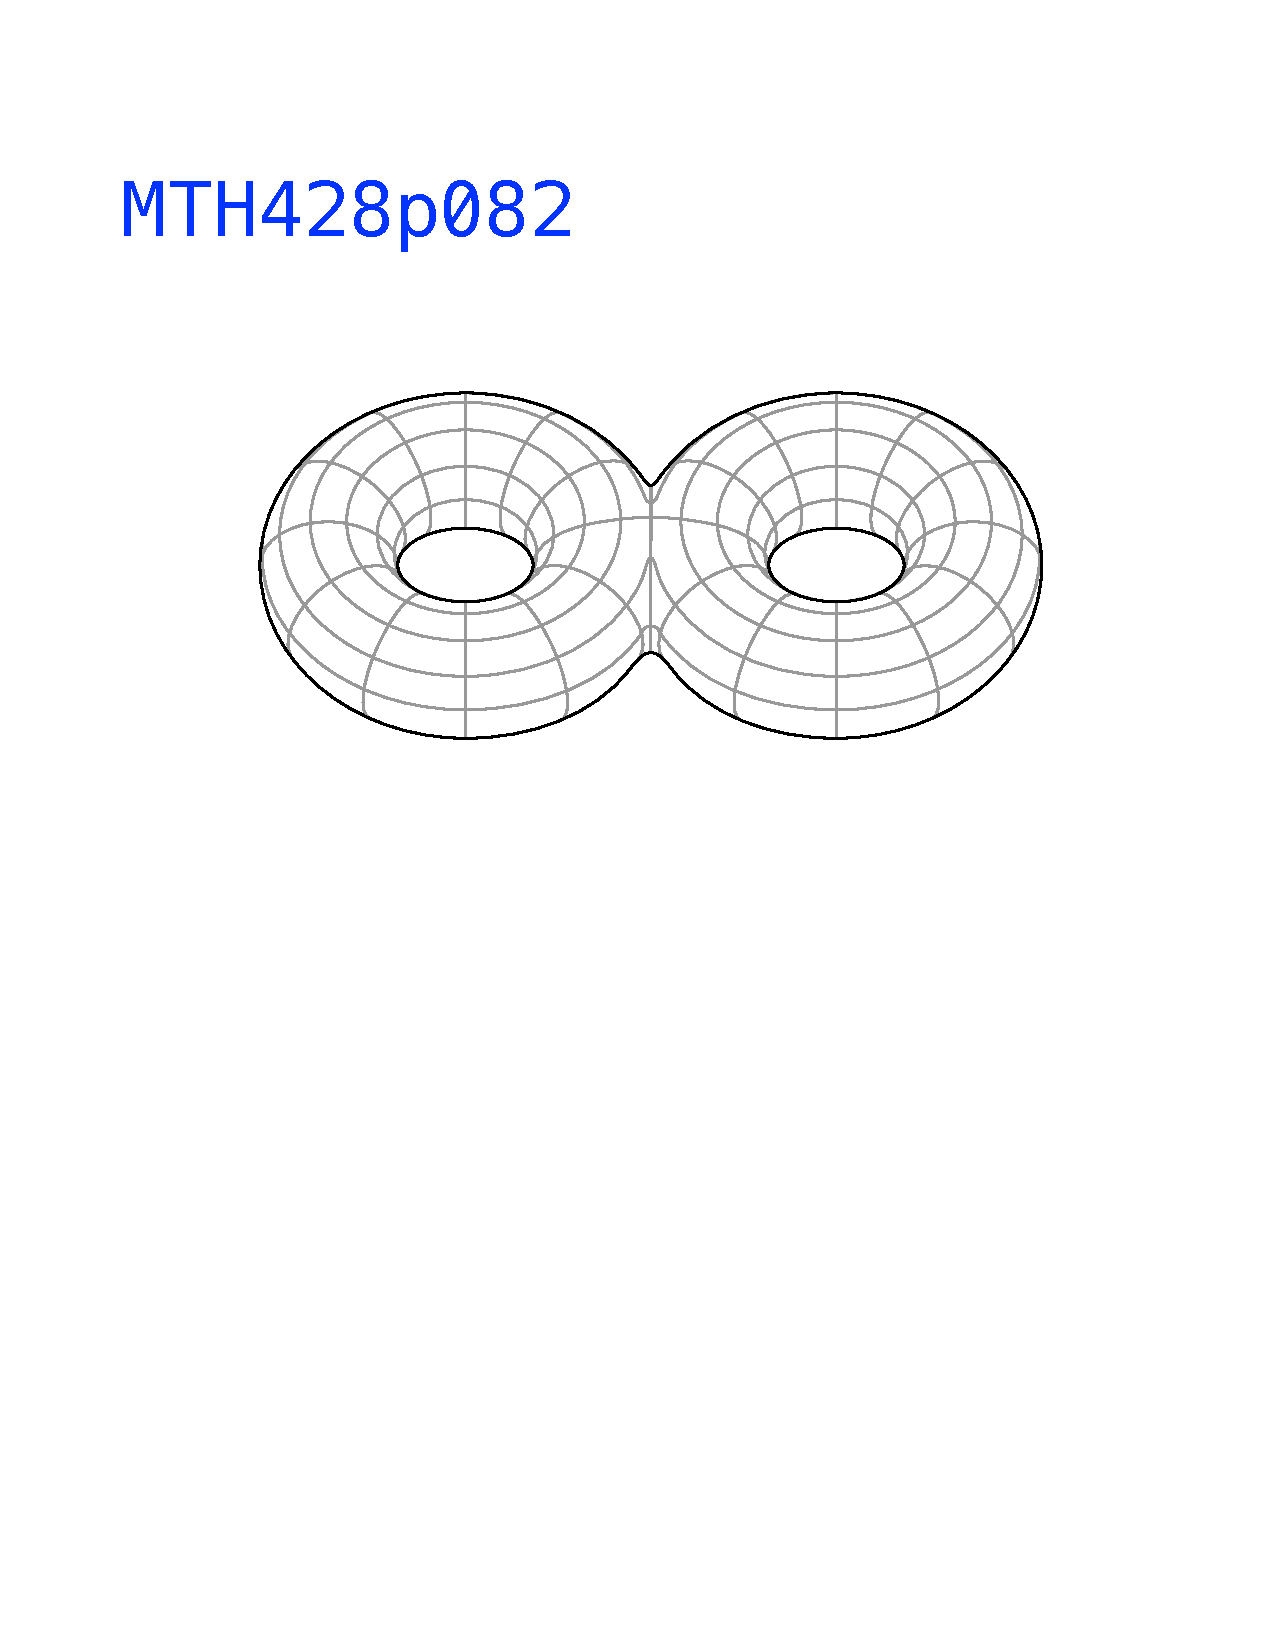
\includegraphics[width=100mm, trim=0mm 153mm 0mm 65mm, clip]{pictures/MTH428p082.pdf}}}
\end{center}

a) Put a CW-complex structure on $T\# T$ and use it to find a presentation of the fundamental group of $T\# T$. 

b) Show that $T\#T$ is not homotopy equivalent to $T$. 

Note: the homeomorphism type of $T\#T$ does not depend on which embedding of 
the disk into $T$ one chooses, so you can work with whichever embedding  is most convenient. 
\end{exercise}


\begin{exercise}
Consider $S^{1}$ as the unit circle in the complex plane 
$$S^{1} = \{z \in \C \  | \ \vert z\vert = 1 \}$$
For $n = 1, 2, \dots$ let $T_{n}$ be a space given by 
$$T_{n} = S^{1}\times [0, 1]/{\sim}$$
where $(z,0)\sim (z^{n}, 1)$ (in particular $T_{1}$ is just a torus). Find the fundamental group of $T_{n}$, and 
show that if $n\neq m$ then $T_{n}$ is not homotopy equivalent to $T_{m}$. 
\end{exercise}

\begin{exercise}
Let $X$ be a 2-dimensional CW-complex. Assume that $X$ has only one 0-cell $x_{0}\in X$.  
Let $(Y, y_{0})$ be a pointed space.  Show that for any group homomorphism 
$\varphi \colon \pi_{1}(X, x_{0}) \to \pi_{1}(Y, y_{0})$ there exists 
a map $f\colon (X, x_{0}) \to (Y, y_{0})$ such that $f_{\ast} = \varphi$. 
\end{exercise}




\newpage
%%%%%%%%%%%%%%%%%%%%%%%%%%%%%%%
%%%%%%%%%%%%%%%%%%%%%%%%%%%%%%%
%%%
%%%  CELLULAR APPROXIMATION THEOREM
%%%
%%%%%%%%%%%%%%%%%%%%%%%%%%%%%%%
%%%%%%%%%%%%%%%%%%%%%%%%%%%%%%%

 %---BBLANK  
\chapter[Cellular Approximation Theorem]{Cellular \\ Approximation \\ Theorem}
 %---EBLANK  
\chaptermark{Cellular Approximation Theorem}
\label{P1CWI CHAPTER}
\thispagestyle{firststyle}

Our next goal will be to develop some methods of computing  fundamental groups of 
arbitrary CW-complexes. The approach we will take is as follows. In this chapter we will establish 
some preliminary results that will  show that the general problem of finding 
the fundamental group of a CW-complex can be reduced to the case of 
CW-complexes of dimension at most 2. We will also describe the structure of fundamental groups 
of 1-dimensional CW-complexes. In order to proceed further we will develop in Chapter 
\ref{PRESENTOFGPS CHAPTER} some convenient algebraic language for describing  
groups in general. This language will be put to use in Chapter \ref{P1CWII CHAPTER} where we will 
continue our investigation of fundamental groups of CW-comolexes. 

 %---BBLANK  
\begin{definition}
Let $X, Y$ be CW-complexes. A map $f\colon X \to Y$ is \emph{cellular} if $f(X^{(n)}) \subseteq Y^{(n)}$
for all $n\geq 0$. 
\end{definition}
 %---EBLANK  # \vskip 30mm

 %---BBLANK  
\begin{CELLAPPROXTHM}
\label{CELLAPPROX THM}
Let $X, Y$ be CW-complexes. For any map $f\colon X \to Y$ there exists a cellular map 
$g\colon X \to Y$ such that $f\simeq g$. Moreover, if $A\subseteq X$ is a subcomplex and 
$f|_{A}\colon A \to Y$ is a cellular map then $g$ can be selected so that   
$f|_{A} = g|_{A}$ and $f\simeq g \ (\rel A)$.
\end{CELLAPPROXTHM}
 %---EBLANK  # \newpage

We will skip the proof of this theorem.  While this result is  of major importance in algebraic topology we will use 
it only once, to prove the following fact:

 %---BBLANK  
\begin{theorem}
\label{FPI12SKINC THM }
Let $X$ be a $CW$-complex and let $x_{0} \in X^{(2)}$. The inclusion map $i\colon X^{(2)} \to X$
induces an isomorphism $i_{\ast}\colon \pi_{1}(X^{(2)}, x_{0}) \to \pi_{1}(X, x_{0})$.
\end{theorem}
 %---EBLANK # \newpage

\begin{proof}
We can assume that $x_{0}$ is a $0$-cell in $X$. We will prove first that $i_{\ast}$ is onto. 
Let $\omega\colon [0, 1] \to X$ be a loop based at $x_{0}$. We need to show that there exists 
a loop $\omega'\colon [0, 1] \to X$ such that $\omega'([0, 1])\subseteq X^{(2)}$ and that 
$\omega\simeq \omega' \ (\rel \{0, 1\})$. 
We can consider the interval $[0, 1]$ as a CW-complex with two $0$-cells joined by one $1$-cell. 
The $0$-skeleton of $[0, 1]$ is the subspace $\{0, 1\}\subseteq [0, 1]$. 
Since  $\omega(0) = \omega(1) = x_{0}\in X^{(0)}$ the map $\omega|_{\{0, 1\}}$ is cellular. 
By Theorem \ref{CELLAPPROX THM} there exists a cellular map $\omega'\colon [0, 1] \to X$
such that $\omega'\simeq \omega \ (\rel \{0, 1\})$. This means that $[\omega] = [\omega']$ 
in $\pi_{1}(X, x_{0})$. Moreover, since $[0, 1]$ is a CW-complex of dimension $1$ thus 
$\omega'$ is a loop in $X^{(1)}\subseteq X^{(2)}$. 
 
 Next, we will show that $i_{\ast}$ is 1-1. Let $[\omega], [\tau]\in \pi_{1}(X^{(2)}, x_{0})$.
Using the same argument as above we can assume that $\omega, \tau \colon [0, 1] \to X^{(2)}$
are cellular maps. Assume that $i_{\ast}([\omega]) = i_{\ast}([\tau])$. This means that 
there exists a path homotopy $h\colon [0, 1]\times [0, 1] \to X$ with $h_{0} = \omega$ 
and $h_{1} = \tau$. The square $I^{2} = [0, 1]\times [0, 1]$ can be considered as a CW-complex  
whose $0$-cells are vertices of the square and whose $1$-cells are the edges.
The 1-skeleton of $I^{2}$ is  the boundary $\partial I^{2}$. Notice that 
$h|_{\partial I^{2}}$ is a cellular map. Using Theorem \ref{CELLAPPROX THM} we obtain that there 
exists a cellular map $h'\colon [0, 1]\times [0, 1] \to X$ such that $h'|_{\partial I^{2}} = h|_{\partial I^{2}}$.  
The map  $h'$ gives another path homotopy between $\omega$ and $\tau$. Moreover, since 
$\dim I^{2} = 2$ thus $h'$ is a homotopy contained in $X^{(2)}$. This shows that 
$[\omega] = [\tau]$ in $\pi_{1}(X^{(2)}, x_{0})$
 
\end{proof}



%%%%%%%%%%%%%%%%%%%%%%%%%%%%%%%
%  EXERCISES
%%%%%%%%%%%%%%%%%%%%%%%%%%%%%%%

\exercises  

\begin{exercise}
Recall that the $n$-dimensional sphere is given by 
$$S^{n} = \{ (x_{1}, \dots, x_{n+1}) \in \R^{n+1} \ | \ x_{1}^{2} + {\dots} + x_{n+1}^{2} = 1\}$$
For $0 \leq m < n$ consider the embedding $i\colon S^{m} \to S^{n}$ given by 
$$i( (x_{1}, \dots, x_{m+1})) = (x_{1}, \dots, x_{m+1}, 0, \dots 0)$$
Using this embedding we can consider  $S^{m}$ as a subspace of $S^{n}$.  Show that the quotient 
space $S^{n}/S^{m}$ is homotopy equivalent to $S^{n}\vee S^{m+1}$. 
(Hint: Proposition \ref{CONTR QUOTIENT WITH HEP PROP} may be useful.)
\end{exercise}



\newpage
%%%%%%%%%%%%%%%%%%%%%%%%%%%%%%%
%%%%%%%%%%%%%%%%%%%%%%%%%%%%%%%
%%%
%%%  COVERING SPACES
%%%
%%%%%%%%%%%%%%%%%%%%%%%%%%%%%%%
%%%%%%%%%%%%%%%%%%%%%%%%%%%%%%%

 %---BBLANK  
\chapter[Covering Spaces]{Covering Spaces}
 %---EBLANK  
\chaptermark{Covering Spaces}

\label{COVERINGSP CHAPTER}

\thispagestyle{firststyle}


 All computations of non-trivial  fundamental groups we have seen use  the fact that the group 
 $\pi_{1}(S^{1})$ is isomorphic to the group of integers. The proof of this fact, however, is still incomplete 
 since it relies on the path lifting property of the universal covering of $S^{1}$ 
 (Proposition \ref{S1 UNIV PATH LIFT PROP})
 that we left without  justification. Our next goal is to fill this gap. In this chapter we  define the notion of 
 a \emph{covering} of a space and we  show that the path lifting property holds for any covering. Since 
 the universal covering of $S^{1}$ is an example of a covering this will give in particular a proof of Proposition 
 \ref{S1 UNIV PATH LIFT PROP}.

 %---BBLANK  
\begin{definition} 
A map $p\colon T\to X$ is a \emph{covering} of $X$ if for every point 
$x\in X$ there exists an open neighborhood $U_{x}\subseteq X$ and a homeomorphism 
$h_{U_{x}}\colon p^{-1}(U_{x}) \to U_{x} \times D_{x}$ where $D_{x}$ is some discrete space, such that the following 
diagram commutes: 
\begin{equation*}
\begin{tikzpicture}
\matrix (m) 
[matrix of math nodes, row sep= 2em, column sep=1.5em, text height=1.5ex, text depth=0.25ex]
{
p^{-1}(U_{x}) & & U_{x} \times D_{x} \\
& U_{x} & \\ 
};
\path[->, thick, font=\scriptsize]
(m-1-1) 
edge node[auto] {$h_{U_{x}}$} (m-1-3)
edge node[anchor=north east] {$p$} (m-2-2)
(m-1-3)
edge node[anchor= north west] {$\pr_{1}$} (m-2-2)
; 
\end{tikzpicture}
\end{equation*}
Here $\pr_{1} \colon U_{x}\times D_{x} \to U_{x}$ is the projection map $\pr_{1}(y, d) = y$. 
\end{definition}
 %---EBLANK  # \newpage


\begin{nn} Here is some terminology and a few comments related to the notion of a covering. 

1) Given a covering $p\colon T\to X$ we will say that $T$ is the \emph{total space}
of $p$ and that $X$ is the \emph{base space}. 

2) For $x\in X$ we have $p^{-1}(x) \cong \{x\} \times D_{x}\cong D_{x}$ which means that $p^{-1}(x)$ is
a discrete space. We call $p^{-1}(x)$ the \emph{fiber} of the covering $p$ over the point $x$. 

3) In general for  $x, x'\in X$ the fibers $p^{-1}(x)$ and $p^{-1}(x')$ may have different numbers
of points, and so they don't need to be homeomorphic. However, if the space $X$ is connected then 
$p^{-1}(x)\cong p^{-1}(x')$ for all $x, x'\in X$ (exercise). 

4) If $p^{-1}(x)$ consists of $n$ points for all $x\in X$ then  we say that $p$ is an $n$-fold covering of $X$. 

5) If $U\subseteq X$ is an open set such that for some discrete space $D$ there exists a homeomorphism 
$h_{U}\colon p^{-1}(U) \to U\times D$ satisfying $\pr_{1}h_{U} = p$ then we say that the set $U$ is 
\emph{evenly covered}. Definition of a covering can be  rephrased by saying that every point $x\in X$
has an open neighborhood which is evenly covered. 

6) If  $U\subseteq X$ is an evenly covered set  and $h_{U}\colon p^{-1}(U) \to U\times D$ is a homeomorphism 
then for $d\in D$ we will say that the set $\nwidetilde{U}_{d} = h^{-1}_{U}(U\times \{d\}) \subseteq p^{-1}(U)$ 
is a \emph{slice} over $U$. The set $p^{-1}(U)$ is then a disjoint union of slices: 

\ 

\begin{tikzpicture}

\node[anchor=south west,inner sep=0] at (0,0) 
{{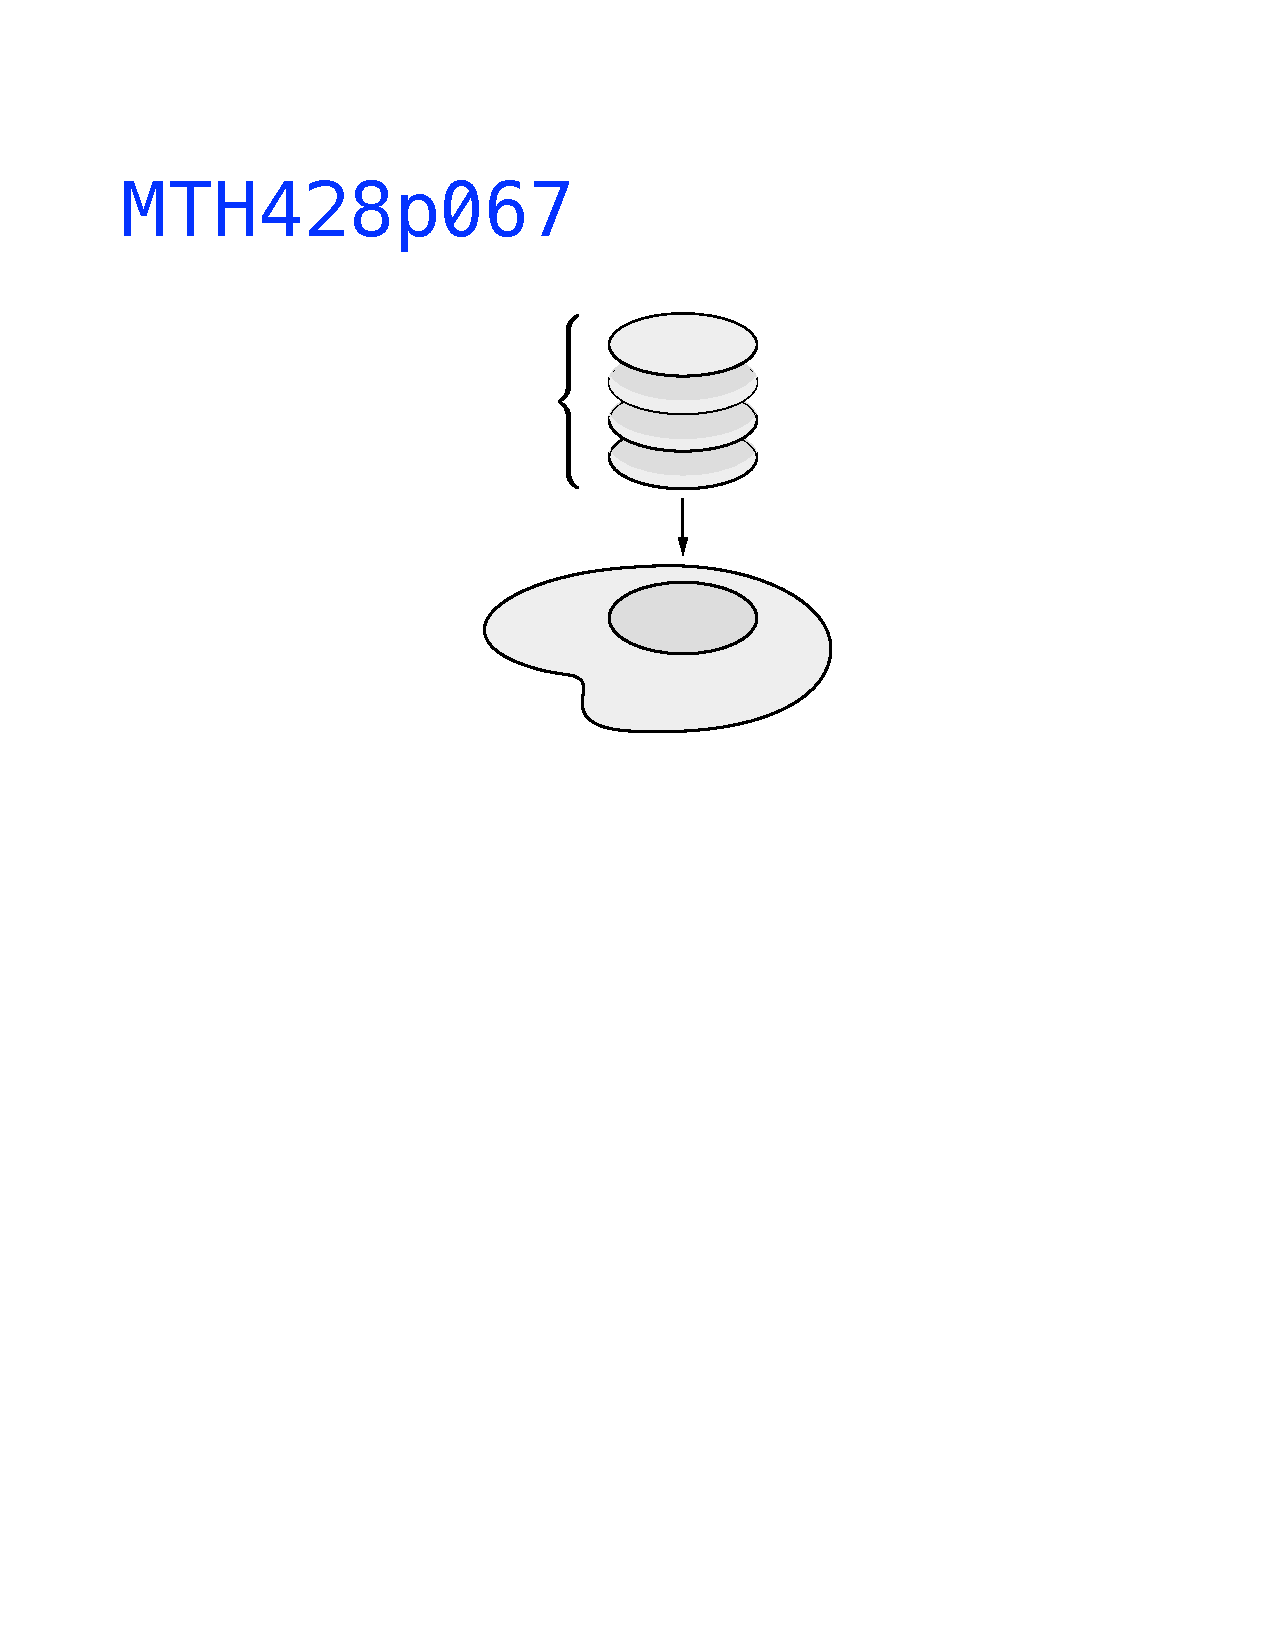
\includegraphics[width=\textwidth, trim=0mm 155mm 0mm 52mm, clip]{pictures/MTH428p067.pdf}}};

%%% COORDINATE GRID
%\draw[step=0.5, help lines] (0,0) to[grid with coordinates] (15,9);
%%% 
\node[anchor= base]  at (6.5 , 4.25){\small  $p^{-1}(U)$};
\node[anchor= base]  at (7.0 , 1.45){\small  $X$};
\node[anchor= base]  at (9.1 , 	2.75){\small  $p$};
\node[anchor= base]  at (8.85 , 1.45){\small $U$};
\node[anchor= base west]  at (9.8 , 4.9){\small $\nwidetilde{U}_{1}$};
\node[anchor= base west]  at (9.8 , 4.4){\small $\nwidetilde{U}_{2}$};
\node[anchor= base west]  at (9.8 , 3.9){\small $\nwidetilde{U}_{3}$};
\node[anchor= base west]  at (9.8 , 3.4){\small $\nwidetilde{U}_{4}$};
\end{tikzpicture}

Moreover, for each slice $\nwidetilde{U}_{d}$ the map $p|_{\nwidetilde{U}_{d}}\colon \nwidetilde{U}_{d} \to U$
is a homeomorphism.  



\end{nn}

 %---BBLANK  
\begin{example}
Let $D$ be a discrete space. The projection map $\pr_{1}\colon X \times D \to X$ is a covering of $X$. 
In this case the whole space $X$ is evenly covered. We say that $\pr_{1}\colon X \times D \to X$ is 
a \emph{trivial covering} of $X$. 
\end{example}
 %---EBLANK  # \vskip 20 mm


 %---BBLANK  
\begin{example}
Recall that the universal covering of $S^{1}$ is the map $p\colon \R^{1} \to S^{1}$ given by 
$p(s) = (\cos 2\pi s, \sin 2\pi s)$. If  $U\subseteq S^{1}$ is  any open set such that $U\neq S^{1}$, 
then $p^{-1}(U)$ is evenly covered and $p^{-1}(U) \cong U\times \Z$ (exercise). 

\

\begin{tikzpicture}

\node[anchor=south west,inner sep=0] at (0,0) 
{{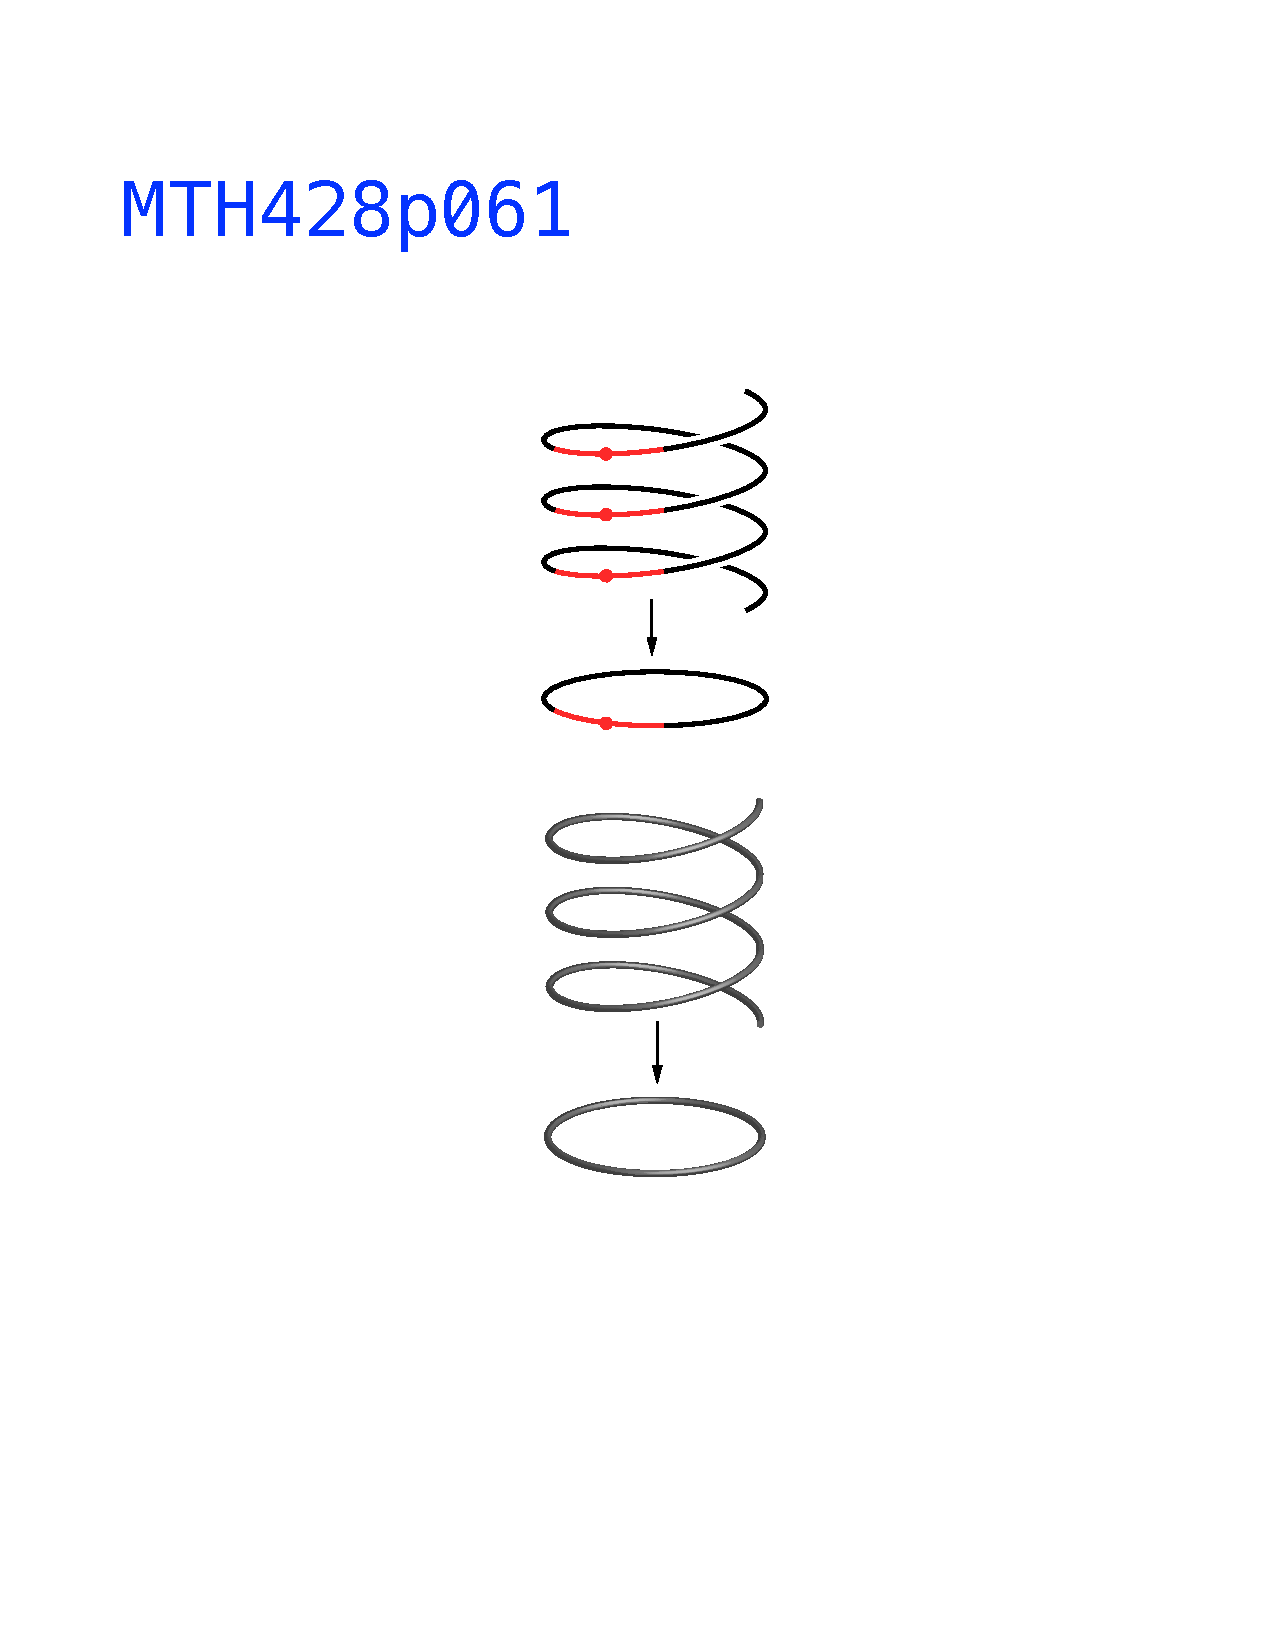
\includegraphics[width=\textwidth, trim=0mm 155mm 0mm 65mm, clip]{pictures/MTH428p061.pdf}}};

%%% COORDINATE GRID
%\draw[step=0.5, help lines] (0,0) to[grid with coordinates] (15,9);
%%% 
\node[anchor= base]  at (7.0 , 4.2){\small  $\R^{1}$};
\node[anchor= base]  at (7.0 , 0.7){\small  $S^{1}$};
\node[anchor= base]  at (8.68 , 	1.45){\small  $p$};
\node[anchor= base]  at (7.85 , -0.15){\small \color{red} $x$};
\node[anchor= base]  at (8.4 , 0.28){\small \color{red} $U$};
\end{tikzpicture}
\end{example}
 %---EBLANK  


 %---BBLANK 
 \begin{example}
Consider $S^{1}$ as a subset of the complex plane:
$$S^{1} = \{z\in \C \ | \ \norm{z} = 1\}$$
For  $n = 1, 2, \dots$ the map $p_{n}\colon S^{1} \to S^{1}$ given by $p_{n}(z) = z^{n}$ is an $n$-fold 
covering of $S^{1}$. Similarly as in the case of the universal covering of $S^{1}$ any open set 
$U\subseteq S^{1}$ such that $U\neq S^{1}$ is evenly covered by $p_{n}$ (exercise).
 

\begin{equation*}
\begin{tikzpicture}[scale = 1.3, 
declare function={
    func(\x)= (\x<= 1.6) * (\x)   +  (\x > 1.6) * (1.6 * 2^( -80*(\x - 1.8) ) /(1 + 2^( -80*(\x - 1.8) ) ) );  
}
]
\begin{axis} [
    view={0}{65},
    axis lines=none,
    ymin=-8,
    ymax=5,
    xmin=-3.5,
    xmax=3.5]
\addplot3 [smooth, line width = 1.4pt, domain=0:2, samples = 1000, samples y=0] ({sin(deg(3*pi*x +1.7))}, {-cos(deg(3*pi*x +1.7))}, {func(x)}) -- cycle;
\addplot3 [smooth, white, line width = 6pt, domain=1.5:2, samples = 200, samples y=0] ({sin(deg(3*pi*x +1.7))}, {-cos(deg(3*pi*x +1.7))}, {func(x)});
\addplot3 [smooth, line width = 1.4pt, domain=1.5:2, samples = 200, samples y=0] ({sin(deg(3*pi*x +1.7))}, {-cos(deg(3*pi*x +1.7))}, {func(x)});
\addplot3 [smooth, white, line width = 6pt, domain=0.5:0.6, samples = 200, samples y=0] ({sin(deg(3*pi*x +1.7))}, {-cos(deg(3*pi*x +1.7))}, {func(x)});
\addplot3 [smooth, line width = 1.4pt, domain=0.5:0.6, samples = 200, samples y=0] ({sin(deg(3*pi*x +1.7))}, {-cos(deg(3*pi*x +1.7))}, {func(x)});
\addplot3 [smooth, white, line width = 6pt, domain=1.2:1.3, samples = 200, samples y=0] ({sin(deg(3*pi*x +1.7))}, {-cos(deg(3*pi*x +1.7))}, {func(x)});
\addplot3 [smooth, line width = 1.4pt, domain=1.2:1.3, samples = 200, samples y=0] ({sin(deg(3*pi*x +1.7))}, {-cos(deg(3*pi*x +1.7))}, {func(x)});
\addplot3 [line width = 1.4pt, domain=0:1, samples = 100, samples y=0, yshift = -40pt] ({sin(deg(2*pi*x))}, {cos(deg(2*pi*x))}, {0})--cycle; 
\end{axis}
\draw[thick,  ->, >=latex ] (3.45,2.2)  -- node[anchor = west, yshift = 2pt] {\small $p_{3}$} (3.45, 1.6) ; 
\node[anchor = west] at (2, 1.5){\small $S^{1}$};
\node[anchor = west] at (2, 4.3){\small $S^{1}$};
\end{tikzpicture}
\end{equation*}

\end{example}
 %---EBLANK  # \newpage


 %---BBLANK 
\begin{example}
If $p_{1}\colon T_{1} \to X_{1}$ and $p_{2}\colon T_{2}\to X_{2}$ are coverings then 
the map $p_{1}\times p_{2}\colon T_{1}\times T_{2} \to X_{1}\times X_{2}$ is also 
a covering (exercise). For example, starting with the universal covering $p\colon \R^{1}\to S^{1}$
of the circle we obtain a covering  $p\times p \colon \R^{1}\times \R^{1} \to S^{1}\times S^{1}$ of the torus. 
\end{example}
 %---EBLANK  # \vskip 30mm

 %---BBLANK 
\begin{example}
Using the coverings of $S^{1}$ described above we can construct  many coverings 
of $S^{1} \vee S^{1}$. For example, here is a covering obtained by combining the universal 
covering over one copy of $S^{1}$ and a trivial covering over the second copy:
 
\begin{tikzpicture}

\node[anchor=south west,inner sep=0] at (0,0) 
{{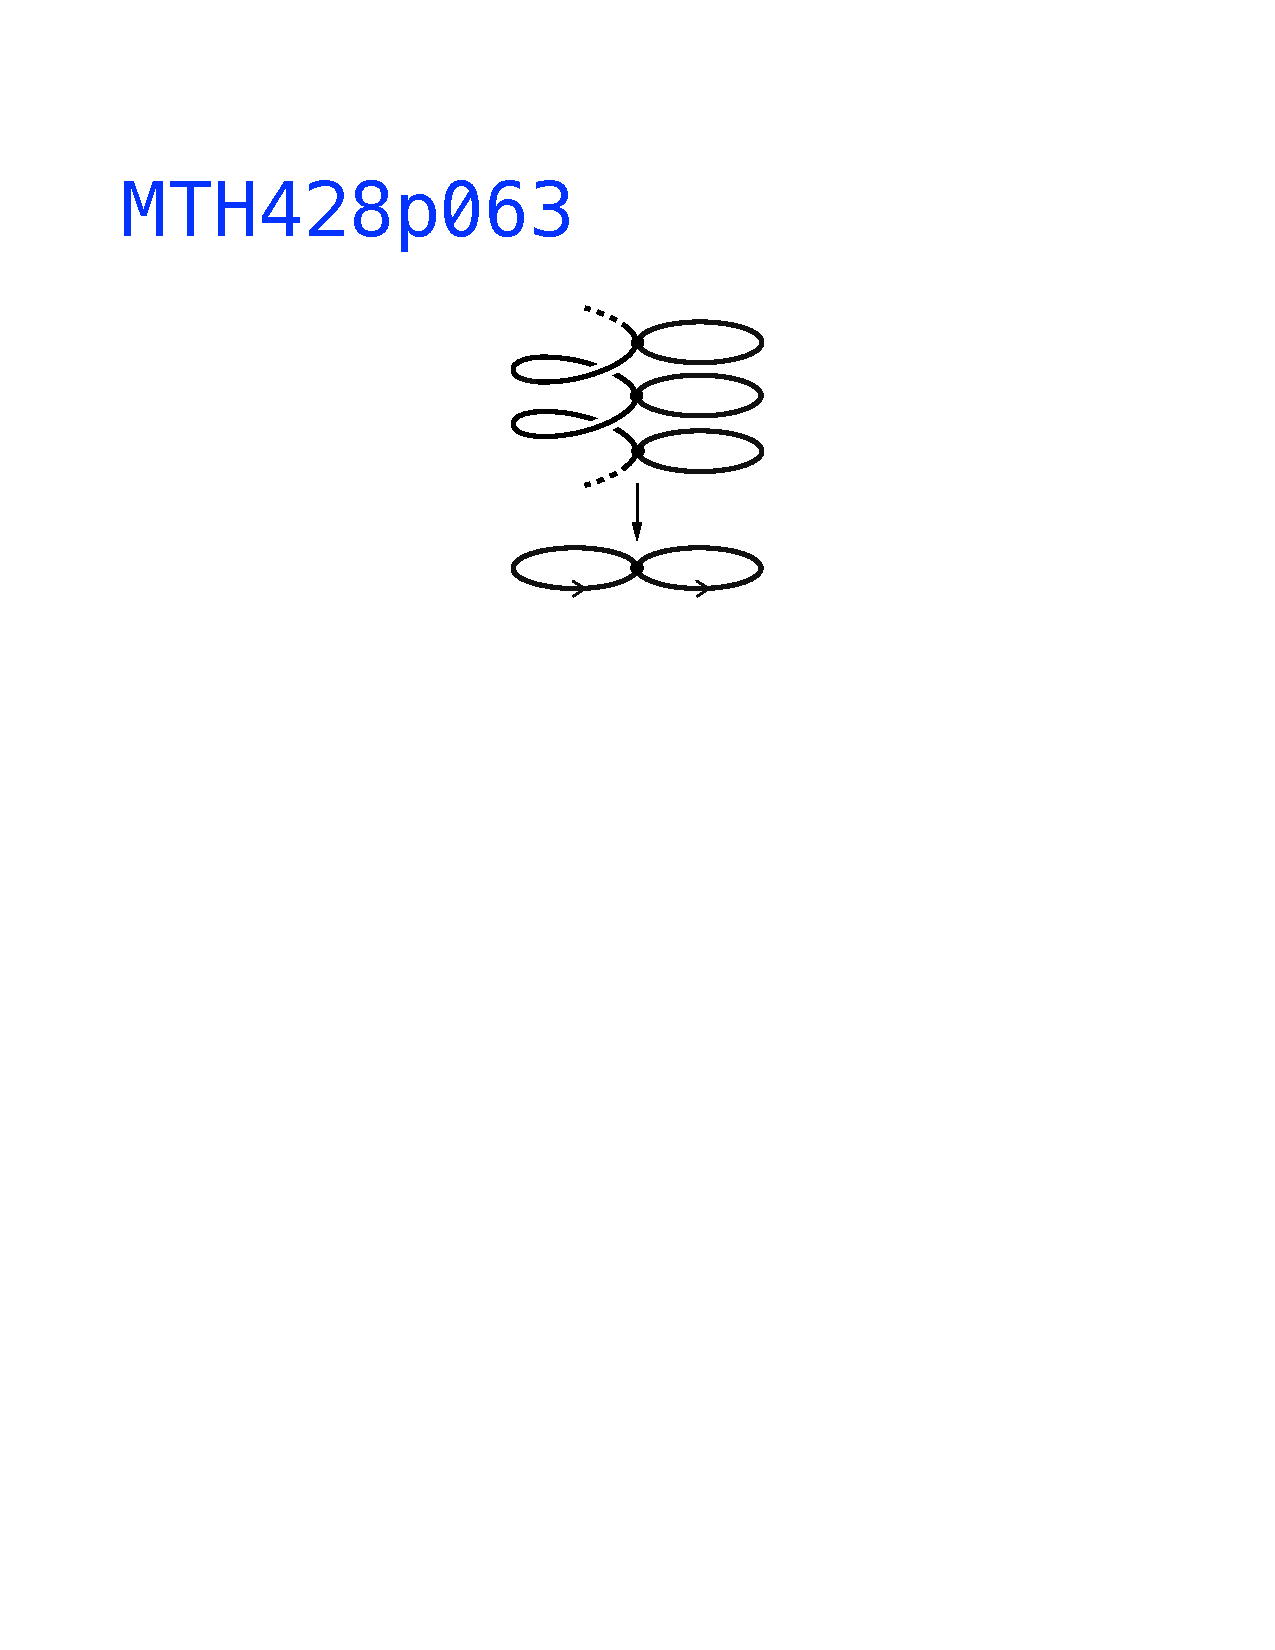
\includegraphics[width=\textwidth, trim=0mm 177mm 0mm 51mm, clip]{pictures/MTH428p063.pdf}}};

%%% COORDINATE GRID
%\draw[step=0.5, help lines] (0,0) to[grid with coordinates] (15,9);
%%% 
\node[anchor= base]  at (7.5 , -0.22){\small  $a$};
\node[anchor= base]  at (9.1 , -0.22){\small  $b$};
\end{tikzpicture}

 %---EBLANK # \end{example}\newpage

Coverings like this  are easier to represent graphically if we untangle the total space 
and indicate which of its parts are being mapped to which copy of $S^{1}$. For the covering 
depicted above this gives:


\begin{equation*}
\begin{tikzpicture}[
    scale = 1.7,
    d0/.style = {line width = 1.6pt},
    d1/.style= {postaction={decorate}, line width = 1.6pt, decoration={markings, mark=at position 0.55 with {\arrow{stealth}}}},
    d2/.style = {postaction={decorate}, line width = 1.6pt, decoration={markings, mark=at position 0.54 with {\arrow[rotate=9]{stealth}}}},
]

\draw[d0, dotted]  (-0.4,0) -- (-0.65,0);
\draw[d0]  (-0.4,0) -- (0,0);
\draw[d1]  (0,0) -- node[anchor= north, pos=0.47, yshift = -2pt] {\small $a$} (1,0);
\draw[d1]  (1,0) -- node[anchor= north, pos=0.47, yshift = -2pt] {\small $a$} (2,0);
\draw[d0]  (2,0) -- (2.4,0);
\draw[d0, dotted]  (2.4,0) -- (2.65,0);
\draw[d2] (0,0) arc (270:-90:0.35) node[anchor= south,  yshift = 1pt, pos= 0.51] {\small $b$} --cycle;
\draw[d2] (1,0) arc (270:-90:0.35) node[anchor= south,  yshift = 1pt, pos= 0.51] {\small $b$} --cycle;
\draw[d2] (2,0) arc (270:-90:0.35) node[anchor= south,  yshift = 1pt, pos= 0.51] {\small $b$} --cycle;
\filldraw (0,0) circle (0.05);
\filldraw (1,0) circle (0.05);
\filldraw (2,0) circle (0.05);
\end{tikzpicture}
\end{equation*}

 %---BBLANK 
Here are two different $3$-fold coverings of $S^{1}\vee S^{1}$:

% first covering
\begin{equation*}
\begin{tikzpicture}[
declare function={
    func(\x)= (\x<= 1.6) * (\x)   +  (\x > 1.6) * (1.6 * 2^( -80*(\x - 1.8) ) /(1 + 2^( -80*(\x - 1.8) ) ) );  
}
]
\begin{scope}
% the next invisible circle is just to center the picture 
\draw[opacity = 0, postaction = {decorate}, red, line width = 1.6pt] (0,0) arc (150:{150+360}:0.25);
\end{scope}

\begin{scope}[xshift = -8mm]
\begin{axis} [
    view={0}{65},
    axis lines=none,
    ymin=-8,
    ymax=5,
    xmin=-3.5,
    xmax=3.5, 
    scale = 0.9]
    
\addplot3 [smooth, line width = 1.6pt, domain=0:2, samples = 1000, samples y=0] ({sin(deg(3*pi*x +1.7))}, {-cos(deg(3*pi*x +1.7))}, {func(x)}) -- cycle;
\addplot3 [smooth, white, line width = 6pt, domain=1.7:1.9, samples = 200, samples y=0] ({sin(deg(3*pi*x +1.7))}, {-cos(deg(3*pi*x +1.7))}, {func(x)});
\addplot3 [smooth, line width = 1.6pt, domain=1.65:1.95, samples = 200, samples y=0] ({sin(deg(3*pi*x +1.7))}, {-cos(deg(3*pi*x +1.7))}, {func(x)});
\addplot3 [smooth, white, line width = 6pt, domain=0.5:0.6, samples = 200, samples y=0] ({sin(deg(3*pi*x +1.7))}, {-cos(deg(3*pi*x +1.7))}, {func(x)});
\addplot3 [smooth, line width = 1.6pt, domain=0.5:0.6, samples = 200, samples y=0] ({sin(deg(3*pi*x +1.7))}, {-cos(deg(3*pi*x +1.7))}, {func(x)});
\addplot3 [smooth, white, line width = 6pt, domain=1.15:1.27, samples = 200, samples y=0] ({sin(deg(3*pi*x +1.7))}, {-cos(deg(3*pi*x +1.7))}, {func(x)});
\addplot3 [smooth, line width = 1.6pt, domain=1.15:1.27, samples = 200, samples y=0] ({sin(deg(3*pi*x +1.7))}, {-cos(deg(3*pi*x +1.7))}, {func(x)});

\addplot3 [line width = 1.6pt, domain=0:1, samples = 100, samples y=0, yshift = -40pt] ({sin(deg(2*pi*x))}, {cos(deg(2*pi*x))}, {0})--cycle; 
\addplot3 [->, >=stealth, line width = 1.6pt, domain=0:-0.5, samples = 100, samples y=0, yshift = -40pt] ({sin(deg(2*pi*x))}, {cos(deg(2*pi*x))}, {0}) node[anchor = base, yshift = -13pt, pos = 0.95] {\small  $a$}; 


\addplot3 [smooth, line width = 1.6pt, domain=0:2, samples = 1000, samples y=0] ({-sin(deg(3*pi*x +1.7))+2}, {-cos(deg(3*pi*x +1.7))}, {func(x)}) -- cycle;
\addplot3 [smooth, white, line width = 6pt, domain=1.7:1.9, samples = 200, samples y=0] ({-sin(deg(3*pi*x +1.7))+2}, {-cos(deg(3*pi*x +1.7))}, {func(x)});
\addplot3 [smooth, line width = 1.6pt, domain=1.65:1.95, samples = 200, samples y=0] ({-sin(deg(3*pi*x +1.7))+2}, {-cos(deg(3*pi*x +1.7))}, {func(x)});
\addplot3 [smooth, white, line width = 6pt, domain=0.5:0.6, samples = 200, samples y=0] ({-sin(deg(3*pi*x +1.7))+2}, {-cos(deg(3*pi*x +1.7))}, {func(x)});
\addplot3 [smooth, line width = 1.6pt, domain=0.5:0.6, samples = 200, samples y=0] ({-sin(deg(3*pi*x +1.7))+2}, {-cos(deg(3*pi*x +1.7))}, {func(x)});
\addplot3 [smooth, white, line width = 6pt, domain=1.2:1.27, samples = 200, samples y=0] ({-sin(deg(3*pi*x +1.7))+2}, {-cos(deg(3*pi*x +1.7))}, {func(x)});
\addplot3 [smooth, line width = 1.6pt, domain=1.2:1.27, samples = 200, samples y=0] ({-sin(deg(3*pi*x +1.7))+2}, {-cos(deg(3*pi*x +1.7))}, {func(x)});


\addplot3 [line width = 1.6pt, domain=0:1, samples = 100, samples y=0, yshift = -40pt] ({-sin(deg(2*pi*x))+2}, {cos(deg(2*pi*x))}, {0})--cycle; 
\addplot3 [->, >=stealth, line width = 1.6pt, domain=0:-0.5, samples = 100, samples y=0, yshift = -40pt] ({sin(deg(2*pi*x))+2}, {cos(deg(2*pi*x))}, {0}) node[anchor = base,  yshift = -13pt, pos = 0.95] {\small  $b$}; 

\addplot3 [thick, ->, >=latex,  yshift = -40pt]  (1,0,1.2) --(1,0,0.4); 

\addplot3 [only marks, mark size = 2, yshift = -40pt] (1,0,0);
\addplot3 [only marks, mark size = 2] (1,0, {pi/2 -1.7/(3*pi) - 4/3});
\addplot3 [only marks, mark size = 2] (1,0, {pi/2 -1.7/(3*pi) - 2/3});
\addplot3 [only marks, mark size = 2] (1,0, {pi/2 -1.7/(3*pi) });

\end{axis}
\end{scope}

% right picture
\begin{scope}[xshift = 85mm, yshift = 22mm, decoration={markings, mark=at position 0.55 with {\arrow{stealth}}}]

\draw[line width = 1.6pt] (0,0) circle (1.65);
\coordinate (a) at ({1.65*sin(0)}, {1.65*cos(0)});
\coordinate (b) at ({1.65*sin(120)}, {1.65*cos(120)});
\coordinate (c) at ({1.65*sin(240)}, {1.65*cos(240)});
\filldraw (a) circle (0.08);
\filldraw (b) circle (0.08);
\filldraw (c) circle (0.08);
\draw[postaction = {decorate}, line width = 1.6pt] (a) -- (b) node[pos = 0.5, anchor = north east, yshift = 1pt] {\small $b$};
\draw[postaction = {decorate}, line width = 1.6pt] (b) -- (c) node[pos = 0.5, anchor = south, yshift = 1pt] {\small $b$};
\draw[postaction = {decorate}, line width = 1.6pt] (c) -- (a) node[pos = 0.5, anchor = north west, xshift = 0pt] {\small $b$};
\draw[postaction = {decorate}, line width = 1.6pt] (b) arc (-30:90:1.65) node[pos = 0.45, anchor = south west, xshift = 1pt] {\small $a$};
\draw[postaction = {decorate}, line width = 1.6pt] (a) arc (90:210:1.65)node[pos = 0.55, anchor = south east] {\small $a$};
\draw[postaction = {decorate}, line width = 1.6pt] (c) arc (210:330:1.65) node[pos = 0.5, anchor = north, yshift = -1pt] {\small $a$};
% the next invisible circle is just to align this picture with the next one 
\draw[opacity = 0, postaction = {decorate}, red, line width = 1.6pt] (b) arc (150:{150+360}:0.5) node[pos = 0.5, anchor = north west, yshift = 2pt] {\small $b$};

\end{scope}

\end{tikzpicture}
\end{equation*}


% second covering
\begin{equation*}
\begin{tikzpicture}[
declare function={
    func(\x)= (\x<= 1.6) * (\x)   +  (\x > 1.6) * (1.6 * 2^( -80*(\x - 1.8) ) /(1 + 2^( -80*(\x - 1.8) ) ) );  
},
declare function={
    func2(\x)= (2/3)*((\x<= 1.4) * (\x)   +  (\x > 1.4) * (1.4 * 2^( -45*(\x - 1.7) ) /(1 + 2^( -45*(\x - 1.7) ) ) )) +2/3;  
}
]
\begin{scope}
% the next invisible circle is just to center the picture 
\draw[opacity = 0, postaction = {decorate}, red, line width = 1.6pt] (0,0) arc (150:{150+360}:0.25);
\end{scope}

\begin{scope}[xshift = -8mm]
\begin{axis} [
    view={0}{65},
    axis lines=none,
    ymin=-8,
    ymax=5,
    xmin=-3.5,
    xmax=3.5, 
    scale = 0.9]
    
\addplot3 [smooth, line width = 1.6pt, domain=0:2, samples = 1000, samples y=0] ({sin(deg(3*pi*x +1.7))}, {-cos(deg(3*pi*x +1.7))}, {func(x)}) -- cycle;
\addplot3 [smooth, white, line width = 6pt, domain=1.7:1.9, samples = 200, samples y=0] ({sin(deg(3*pi*x +1.7))}, {-cos(deg(3*pi*x +1.7))}, {func(x)});
\addplot3 [smooth, line width = 1.6pt, domain=1.65:1.95, samples = 200, samples y=0] ({sin(deg(3*pi*x +1.7))}, {-cos(deg(3*pi*x +1.7))}, {func(x)});
\addplot3 [smooth, white, line width = 6pt, domain=0.5:0.6, samples = 200, samples y=0] ({sin(deg(3*pi*x +1.7))}, {-cos(deg(3*pi*x +1.7))}, {func(x)});
\addplot3 [smooth, line width = 1.6pt, domain=0.5:0.6, samples = 200, samples y=0] ({sin(deg(3*pi*x +1.7))}, {-cos(deg(3*pi*x +1.7))}, {func(x)});
\addplot3 [smooth, white, line width = 6pt, domain=1.15:1.27, samples = 200, samples y=0] ({sin(deg(3*pi*x +1.7))}, {-cos(deg(3*pi*x +1.7))}, {func(x)});
\addplot3 [smooth, line width = 1.6pt, domain=1.15:1.27, samples = 200, samples y=0] ({sin(deg(3*pi*x +1.7))}, {-cos(deg(3*pi*x +1.7))}, {func(x)});

\addplot3 [line width = 1.6pt, domain=0:1, samples = 100, samples y=0, yshift = -40pt] ({sin(deg(2*pi*x))}, {cos(deg(2*pi*x))}, {0})--cycle; 
\addplot3 [->, >=stealth, line width = 1.6pt, domain=0:-0.5, samples = 100, samples y=0, yshift = -40pt] ({sin(deg(2*pi*x))}, {cos(deg(2*pi*x))}, {0}) node[anchor = base, yshift = -13pt, pos = 0.95] {\small  $a$}; 


\addplot3 [smooth, line width = 1.6pt, domain=0:2, samples = 1000, samples y=0] ({-sin(deg(2*pi*x +1.95))+2}, {-cos(deg(2*pi*x +1.95))}, {func2(x)}) -- cycle;
\addplot3 [smooth, white, line width = 6pt, domain=0.72:0.85, samples = 200, samples y=0] ({-sin(deg(2*pi*x +1.95))+2}, {-cos(deg(2*pi*x +1.95))}, {func2(x)});
\addplot3 [smooth, line width = 1.6pt, domain=0.72:0.85, samples = 200, samples y=0] ({-sin(deg(2*pi*x +1.95))+2}, {-cos(deg(2*pi*x +1.95))}, {func2(x)});
\addplot3 [smooth, white, line width = 6pt, domain=1.8:1.6, samples = 200, samples y=0] ({-sin(deg(2*pi*x +1.95))+2}, {-cos(deg(2*pi*x +1.95))}, {func2(x)});
\addplot3 [smooth, line width = 1.6pt, domain=1.8:1.6, samples = 200, samples y=0] ({-sin(deg(2*pi*x +1.95))+2}, {-cos(deg(2*pi*x +1.95))}, {func2(x)});

\addplot3 [line width = 1.6pt, domain=0:1, samples = 100, samples y=0] ({-sin(deg(2*pi*x))+2}, {cos(deg(2*pi*x))}, {pi/2 -1.7/(3*pi) - 4/3})--cycle; 


\addplot3 [line width = 1.6pt, domain=0:1, samples = 100, samples y=0, yshift = -40pt] ({-sin(deg(2*pi*x))+2}, {cos(deg(2*pi*x))}, {0})--cycle; 
\addplot3 [->, >=stealth, line width = 1.6pt, domain=0:-0.5, samples = 100, samples y=0, yshift = -40pt] ({sin(deg(2*pi*x))+2}, {cos(deg(2*pi*x))}, {0}) node[anchor = base,  yshift = -13pt, pos = 0.95] {\small  $b$}; 


\addplot3 [thick, ->, >=latex,  yshift = -40pt]  (1,0,1.2) --(1,0,0.4); 

\addplot3 [only marks, mark size = 2, yshift = -40pt] (1,0,0);
\addplot3 [only marks, mark size = 2] (1,0, {pi/2 -1.7/(3*pi) - 4/3});
\addplot3 [only marks, mark size = 2] (1,0, {pi/2 -1.7/(3*pi) - 2/3});
\addplot3 [only marks, mark size = 2] (1,0, {pi/2 -1.7/(3*pi) });

\end{axis}
\end{scope}

% right picture
\begin{scope}[xshift = 85mm, yshift = 22mm]

\tikzset{
    d1/.style= {line width = 1.6pt, decoration={markings, mark=at position 0.55 with {\arrow{stealth}}}},
    d2/.style = {line width = 1.6pt, decoration={markings, mark=at position 0.55 with {\arrow[rotate=-10]{stealth}}}},
}


\draw[line width = 1.6pt] (0,0) circle (1.65);
\coordinate (a) at ({1.65*sin(0)}, {1.65*cos(0)});
\coordinate (b) at ({1.65*sin(120)}, {1.65*cos(120)});
\coordinate (c) at ({1.65*sin(240)}, {1.65*cos(240)});
\filldraw (a) circle (0.08);
\filldraw (b) circle (0.08);
\filldraw (c) circle (0.08);
\draw[postaction = {decorate}, d1] (a) -- (c) node[pos = 0.5, anchor = north west, yshift = 0pt] {\small $b$};
\draw[postaction = {decorate}, d1] (c) arc (270:390:1.65) node[pos = 0.5, anchor = north west, yshift = 0pt] {\small $b$};
\draw[postaction = {decorate}, d2] (b) arc (150:{150+360}:0.5) node[pos = 0.5, anchor = north west, yshift = 2pt] {\small $b$};


\draw[postaction = {decorate}, d1] (b) arc (-30:90:1.65) node[pos = 0.45, anchor = south west, xshift = 1pt] {\small $a$};
\draw[postaction = {decorate}, d1] (a) arc (90:210:1.65)node[pos = 0.52, anchor = south east] {\small $a$};
\draw[postaction = {decorate}, d1] (c) arc (210:330:1.65) node[pos = 0.5, anchor = north, yshift = -2pt] {\small $a$};
\end{scope}

\end{tikzpicture}
\end{equation*}
 %---EBLANK  # \newpage


\end{example}


 %---BBLANK 
\begin{definition}
If $p\colon T \to X$ is a covering and $f\colon Y \to X$ is a map then a \emph{lift} of $f$
is a map $\ntilde{f}\colon Y\to T$ such that the following diagram commutes:
\begin{center}
\begin{tikzpicture}
\matrix (m) 
[matrix of math nodes, row sep= 2.5em, column sep=3em, text height=1.5ex, text depth=0.25ex]
{
   &  T \\
Y & X & \\ 
};
\path[->, thick, font=\scriptsize]
(m-2-1) 
edge node[auto] {$\ntilde{f}$} (m-1-2)
edge node[below] {$f$} (m-2-2)
(m-1-2) 
edge node[auto] {$p$} (m-2-2)
;
\end{tikzpicture}
\end{center}
\end{definition}
 %---EBLANK 


The following fact describes one of the main properties of coverings:


 %---BBLANK  # \vskip 30mm
\begin{COVHOMOTLIFTTHM}
\label{HOMOTOPYLIFT THM}
Let $p\colon T\to X$ be a covering. Let $F\colon Y \times [0, 1] \to X$ and 
$\ntilde{f} \colon Y\times \{0\} \to T$ be functions satisfying $p\ntilde{f} = F|_{Y\times \{0\}}$.  
There exists a function $\nwidetilde{F}\colon Y \times [0, 1] \to T$ such that $p\nwidetilde{F}  = F$
and $\nwidetilde{F}|_{Y\times \{0\}} = \ntilde{f}$: 
\begin{equation*}
\label{HOMOTLIFTCOV EQ}
\tag{$\ast$}
\begin{tikzpicture}[baseline=(current  bounding  box.center)]
\matrix (m) 
[matrix of math nodes, row sep= 3em, column sep=3.5em, text height=1.5ex, text depth=0.25ex]
{
Y\times \{0\}  &  T \\
Y\times [0, 1] & X & \\ 
};
\path[->, thick, font=\scriptsize]
(m-1-1) 
edge node[auto] {$\ntilde{f}$} (m-1-2)
(m-1-2)
edge node[anchor=  west] {$p$} (m-2-2)
(m-2-1)
edge node[anchor= north] {$F$} (m-2-2)
; 
\path[right hook ->, thick, font=\scriptsize]
(m-1-1) 
edge node[anchor=north east] {} (m-2-1)
;
\path[->, thick, dashed, font=\scriptsize]
(m-2-1.20)
edge node[anchor= south east] {$\nwidetilde{F}$} (m-1-2)
;
\end{tikzpicture}
\end{equation*}
Moreover, such function $\nwidetilde{F}$ is unique.  
\end{COVHOMOTLIFTTHM}
 %---EBLANK  # \newpage


Before we get to the proof of  this theorem we will show that it implies that any covering has path lifting properties 
analogous to the ones described in Proposition \ref{S1 UNIV PATH LIFT PROP}  for the universal covering of $S^{1}$:


 %---BBLANK 
\begin{corollary}
\label{COVERING PATH LIFT COR} 
Let $p\colon T \to X$ be a  covering.  Let $x_{0}\in X$, and let  $\ntilde{x}_{0}\in T$ 
be a point such that $p(\ntilde{x}_{0}) = x_{0}$. 

1) For any path $\omega\colon [0,1]\to X$ such that $\omega(0) = x_{0}$ there exists a lift 
$\nwidetilde{\omega}\colon [0, 1]\to T$ satisfying $\nwidetilde{\omega}(0) = \ntilde{x}_{0}$. Moreover, 
such lift is unique. 


2) Let $\omega, \tau\colon [0, 1]\to X$ be paths such that $\omega(0) = \tau(0) = x_{0}$, 
$\omega(1) = \tau(1)$ and $\omega\simeq \tau$. If  
$\nwidetilde\omega$, $\nwidetilde\tau$ are lifts of $\omega$,  $\tau$, respectively, such that 
$\nwidetilde{\omega}(0) = \nwidetilde{\tau}(0) = \ntilde{x}_{0}$ then 
$\nwidetilde{\omega}(1) = \nwidetilde{\tau}(1)$ and $\nwidetilde{\omega}\simeq \nwidetilde{\tau}$. 

\end{corollary}
 %---EBLANK  # \newpage


\begin{proof}
For part 1)  let $Y = \{\ast\}$ be the space consisting of one point. We can consider the path $\omega$ 
as a map $\omega\colon \{\ast\} \times [0, 1] \to X$. Denote  by $c_{\ntilde{x}_{0}}\colon  \{\ast\} \times \{0\} \to T$ the  
map given by $c_{\ntilde{x}_{0}}(\ast, 0) = \ntilde{x}_{0}$. We have a commutative diagram: 
\begin{equation*}
\begin{tikzpicture}
\matrix (m) 
[matrix of math nodes, row sep= 3em, column sep=3.5em, text height=1.5ex, text depth=0.25ex]
{
\{\ast\} \times \{0\}  &  T \\
\{\ast\}\times [0, 1] & X & \\ 
};
\path[->, thick, font=\scriptsize]
(m-1-1) 
edge node[auto] {$c_{\ntilde{x}_{0}}$} (m-1-2)
(m-1-2)
edge node[anchor=  west] {$p$} (m-2-2)
(m-2-1)
edge node[anchor= north] {$\omega$} (m-2-2)
; 
\path[right hook ->, thick, font=\scriptsize]
(m-1-1) 
edge node[anchor=north east] {} (m-2-1)
;
\end{tikzpicture}
\end{equation*}
By Theorem \ref{HOMOTOPYLIFT THM}   there exists a unique map 
$\nwidetilde{\omega} \colon \{\ast\}\times [0, 1] \to T$ which gives the desired lift of $\omega$. 

Part 2) is  an exercise. 

\end{proof}

Proof of Theorem \ref{HOMOTOPYLIFT THM} will use a couple of lemmas. The first of them if 
of interest of its own right:


 %---BBLANK 
\begin{lemma}
\label{COVERINGUNIQUELIFT LEMMA}
Let $p\colon T\to X$ be a covering, and let $\ntilde{f}_{1}, \ntilde{f}_{2}\colon Y \to T$ be two lifts of 
a map $f\colon Y\to X$. If $Y$ is a connected space and there exists $y_{0}\in Y$ such that 
$\ntilde{f}_{1}(y_{0}) = \ntilde{f}_{2}(y_{0})$ then $\ntilde{f}_{1}(y) = \ntilde{f}_{2}(y)$ for all $y\in Y$. 
\begin{equation*}
\begin{tikzpicture}
\matrix (m) 
[matrix of math nodes, row sep= 3em, column sep=4.5em, text height=1.5ex, text depth=0.25ex]
{
   &  T \\
Y & X & \\ 
};
\path[->, thick, font=\scriptsize]
(m-1-2)
edge node[anchor=  west] {$p$} (m-2-2)
(m-2-1)
edge node[anchor= north] {$f$} (m-2-2)
; 
\path[->, thick, transform canvas = {xshift = -0.3ex, yshift = 0.3ex}, font=\scriptsize]
(m-2-1.50)
edge node[anchor= south east] {$\ntilde{f}_{1}$} (m-1-2.200)
;
\path[->, thick, transform canvas = {xshift = 0.3ex, yshift = -0.3ex}, font=\scriptsize]
(m-2-1.50)
edge node[anchor= north west] {$\ntilde{f}_{2}$} (m-1-2.200)
;
\end{tikzpicture}
\end{equation*}
\end{lemma}
 %---EBLANK  # \newpage

\begin{proof}
Let $Y_{e}, Y_{n}\subseteq X$ be sets defined by 
$$Y_{e} = \{y\in Y \ | \ \ntilde{f}_{1}(y) = \ntilde{f}_{2}(y) \} 
\ \ \ \ \text{and} \ \ \ \  Y_{n} = \{y\in Y \ | \ \ntilde{f}_{1}(y) \neq \ntilde{f}_{2}(y) \}$$
Notice that $Y_{e}\cup Y_{n} = Y$ and $Y_{e}\cap Y_{n} = \varnothing$. Notice also that 
$Y_{e}\neq \varnothing$ since $y_{0}\in Y_{e}$. It will be enough to show that $Y_{e}$ and $Y_{n}$
are open in $Y$. By connectedness of $Y$ this will imply that $Y_{e} = Y$. 

To see that $Y_{e}$ is open take $y\in Y_{e}$. It will suffice to show that there exists an open 
set $V\subseteq Y$ such that $y\in V$ and $V\subseteq Y_{e}$. Let $U\subseteq X$ be an evenly covered 
open neighborhood of $f(y)$ and let $\nwidetilde{U}$ be a slice over $U$ such that 
$\ntilde{f}_{1}(y) = \ntilde{f}_{2}(y) \in \nwidetilde{U}$.

\begin{tikzpicture}

\node[anchor=south west,inner sep=0] at (0,0) 
{{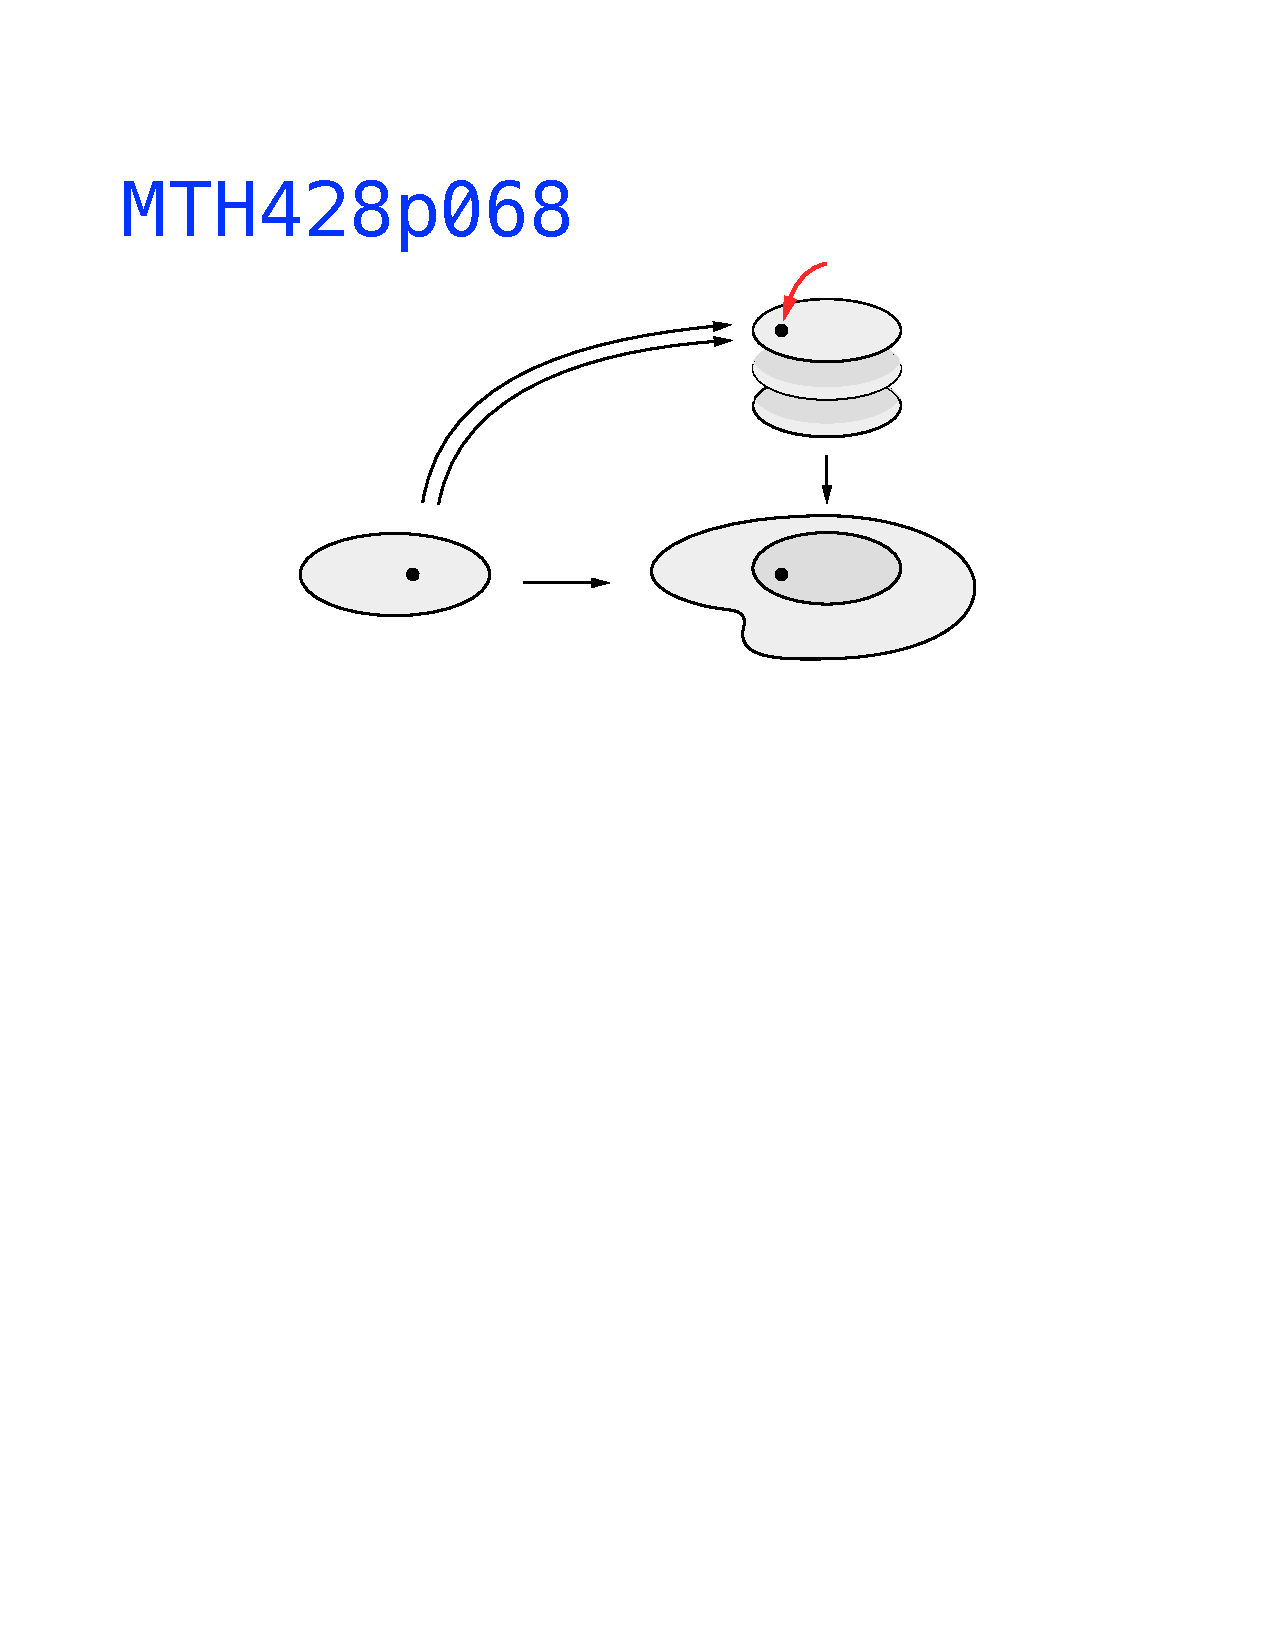
\includegraphics[width=\textwidth, trim=0mm 167mm 0mm 44mm, clip]{pictures/MTH428p068.pdf}}};

%%% COORDINATE GRID
%\draw[step=0.5, help lines] (0,0) to[grid with coordinates] (15,9);
%%% 
\node[anchor= base]  at (7.35 , 1.2){\small  $f$};
\node[anchor= base]  at (10.95 , 2.4){\small  $p$};
\node[anchor= base]  at (6.8 , 4.0){\small  $\ntilde{f}_{1}$};
\node[anchor= base]  at (7.2 , 3.25){\small  $\ntilde{f}_{2}$};
\node[anchor= base]  at (5.6 , 1.09){\small $y$};
\node[anchor= base]  at (10.55 , 1.09){\small $f(y)$};
\node[anchor= base west]  at (10.7 , 5.1){\small $\ntilde{f}_{1}(y) = \ntilde{f}_{2}(y)$};
\node[anchor= base west]  at (11.64 , 4.3){\small $\nwidetilde{U}$};
\node[anchor= base west]  at (11.64 , 1.15){\small $U$};
\node[anchor= base]  at (4.0 , 1.6){\small $Y$};
\node[anchor= base west]  at (12.3 , 1.6){\small $X$};

\end{tikzpicture}

Take $V = \ntilde{f}_{1}^{-1}(\nwidetilde{U}) \cap \ntilde{f}_{2}^{-1}(\nwidetilde{U})$. The set $V$ is an open 
neighborhood of $y$. Also, for $y'\in V$ we have 
$$p|_{\nwidetilde{U}}\circ \ntilde{f}_{1}(y') = f(y') = p|_{\nwidetilde{U}}\circ \ntilde{f}_{2}(y')$$
Since $p|_{\nwidetilde{U}}\colon \nwidetilde{U} \to U$ is a homeomorphism  this gives 
$\ntilde{f}_{1}(y') =  \ntilde{f}_{2}(y')$,  and so $y'\in Y_{e}$. 

Openness of $Y_{n}$ can be verified in a similar way (exercise).
\end{proof}

The next lemma is a special case of Theorem \ref{HOMOTOPYLIFT THM}:


 %---BBLANK 
\begin{lemma}
\label{EVENCOVERHOMOTLIFT LEMMA}
Let $p\colon T\to X$ be a covering. Let $F\colon Y \times [a, b] \to X$ and 
$\ntilde{f} \colon Y\times \{a\} \to T$ be functions satisfying $p\ntilde{f} = F|_{Y\times \{a\}}$.  
Assume also that $F(Y \times [a, b]) \subseteq U$ where $U\subseteq X$ is an evenly covered 
open set. There exists a function $\nwidetilde{F}\colon Y \times [a, b] \to T$ such that $p\nwidetilde{F}  = F$
and $\nwidetilde{F}|_{Y\times \{a\}} = \ntilde{f}$: 
\begin{equation*}
\begin{tikzpicture}[baseline=(current  bounding  box.center)]
\matrix (m) 
[matrix of math nodes, row sep= 3em, column sep=3.5em, text height=1.5ex, text depth=0.25ex]
{
Y\times \{a\}  &  T \\
Y\times [a, b] & X & \\ 
};
\path[->, thick, font=\scriptsize]
(m-1-1) 
edge node[auto] {$\ntilde{f}$} (m-1-2)
(m-1-2)
edge node[anchor=  west] {$p$} (m-2-2)
(m-2-1)
edge node[anchor= north] {$F$} (m-2-2)
; 
\path[right hook ->, thick, font=\scriptsize]
(m-1-1) 
edge node[anchor=north east] {} (m-2-1)
;
\path[->, thick, dashed, font=\scriptsize]
(m-2-1.20)
edge node[anchor= south east] {$\nwidetilde{F}$} (m-1-2)
;
\end{tikzpicture}
\end{equation*}
\end{lemma}
 %---EBLANK  # \newpage


\begin{proof}
Let $\{\nwidetilde{U}_{i}\}_{i\in I}$ be the set of slices of $p$ over the set $U$, and let 
$V_{i} = \{y\in Y \ | \ \ntilde{f}(y, a) \in \nwidetilde{U}_{i}\}$. The sets $V_{i} \times [a, b]$ form an 
open cover of $Y\times [a, b]$. Since for each $i\in I$ the map $p|_{\nwidetilde{U}_{i}} \colon \nwidetilde{U}_{i} \to U$
is a homeomorphism we can define 
$$\nwidetilde{F}|_{V_{i}\times [a, b]} = (p|_{\nwidetilde{U}_{i}})^{-1}\circ  F|_{V_{i}\times [a, b]}$$
Since for $i\neq j$ we have $V_{i}\cap V_{j} = \varnothing$ this gives a well defined continuous function
$\nwidetilde{F} \colon Y\times [a, b] \to T$
\end{proof}



 %---BBLANK 
\begin{proof}[Proof of Theorem \ref{HOMOTOPYLIFT THM}] 
 %---EBLANK  # \end{proof} \newpage
 
We will  show first that if the map $\nwidetilde{F}$
exists then it must be unique. Assume that for $i=1, 2$ we have a map $\nwidetilde{F}_{i}$ such that 
the following diagram commutes:
\begin{equation*}
\begin{tikzpicture}[baseline=(current  bounding  box.center)]
\matrix (m) 
[matrix of math nodes, row sep= 3em, column sep=3.5em, text height=1.5ex, text depth=0.25ex]
{
Y\times \{0\}  &  T \\
Y\times [0, 1] & X & \\ 
};
\path[->, thick, font=\scriptsize]
(m-1-1) 
edge node[auto] {$\ntilde{f}$} (m-1-2)
(m-1-2)
edge node[anchor=  west] {$p$} (m-2-2)
(m-2-1)
edge node[anchor= north] {$F$} (m-2-2)
; 
\path[right hook ->, thick, font=\scriptsize]
(m-1-1) 
edge node[anchor=north east] {} (m-2-1)
;
\path[->, thick, dashed, font=\scriptsize]
(m-2-1.20)
edge node[anchor= south east] {$\nwidetilde{F}_{i}$} (m-1-2)
;
\end{tikzpicture}
\end{equation*}
Take $y\in Y$. Notice that the set $\{y\}\times [0, 1] \subseteq Y \times [0, 1]$ is connected, for 
$i=1, 2$ the map $\nwidetilde{F}_{i}|_{\{y\}\times [0, 1]}$ is a lift of $F|_{\{y\}\times [0, 1]}$, and 
$\nwidetilde{F}_{1}|_{\{y\}\times [0, 1]}(y, 0) = \ntilde{f}(y, 0) = \nwidetilde{F}_{2}|_{\{y\}\times [0, 1]}(y, 0)$. 
By Lemma \ref{COVERINGUNIQUELIFT LEMMA} we obtain  that 
$\nwidetilde{F}_{1}|_{\{y\}\times [0, 1]} = \nwidetilde{F}_{2}|_{\{y\}\times [0, 1]}$ for each $y\in Y$. Therefore
$\nwidetilde{F}_{1} = \nwidetilde{F}_{2}$.  

It remains to show that a map $\nwidetilde{F}$ in the diagram (\ref{HOMOTLIFTCOV EQ}) exists. 
Let $y\in Y$. We will construct first a map $\nwidetilde{F}_{{y}}\colon V_{y}\times [0, 1] \to T$ where 
$V_{y}\subseteq Y$ is some open neighborhood of $y$,  such that the following diagram commutes:
\begin{equation*}
\label{HOMOTOPYLIFTTHMPF EQ1}
\tag{$\ast\ast$}
\begin{tikzpicture}[baseline=(current  bounding  box.center)]
\matrix (m) 
[matrix of math nodes, row sep= 3em, column sep=4.5em, text height=1.5ex, text depth=0.25ex]
{
V_{y}\times \{0\}  &  T \\
V_{y}\times [0, 1] & X & \\ 
};
\path[->, thick, font=\scriptsize]
(m-1-1) 
edge node[auto] {$\ntilde{f}|_{V_{y}\times \{0\}}$} (m-1-2)
(m-1-2)
edge node[anchor=  west] {$p$} (m-2-2)
(m-2-1)
edge node[anchor= north] {$F|_{V_{y}\times [0, 1]}$} (m-2-2)
; 
\path[right hook ->, thick, font=\scriptsize]
(m-1-1) 
edge node[anchor=north east] {} (m-2-1)
;
\path[->, thick, dashed, font=\scriptsize]
(m-2-1.20)
edge node[anchor= south east] {$\nwidetilde{F}_{{y}}$} (m-1-2)
;
\end{tikzpicture}
\end{equation*}
The construction of $\nwidetilde{F}_{y}$ proceeds as follows. Using compactness of the interval $[0, 1]$ we can find
an open neighborhood $V_{y} \subseteq Y$ of $y$ and numbers $0= t_{0} < t_{1} < {\dots} < t_{n} = 1$
such that for each $i=1, \dots, n$ we have  $F(V_{y}\times [t_{i-1}, t_{i}]) \subseteq U_{i}$ where 
$U_{i}\subseteq X$ is an evenly covered open set.  Using Lemma \ref{EVENCOVERHOMOTLIFT LEMMA}
we obtain a map  $\nwidetilde{F}_{y, 1}\colon V_{y}\times [t_{0}, t_{1}] \to T$ that gives a commutative 
diagram 
\begin{equation*}
\begin{tikzpicture}[baseline=(current  bounding  box.center)]
\matrix (m) 
[matrix of math nodes, row sep= 3em, column sep=4.5em, text height=1.5ex, text depth=0.25ex]
{
V_{y}\times \{0\}  &  T \\
V_{y}\times [t_{0}, t_{1}] & X & \\ 
};
\path[->, thick, font=\scriptsize]
(m-1-1) 
edge node[auto] {$\ntilde{f}|_{V_{y}\times \{0\}}$} (m-1-2)
(m-1-2)
edge node[anchor=  west] {$p$} (m-2-2)
(m-2-1)
edge node[anchor= north] {$F|_{V_{y}\times [t_{0}, t_{1}]}$} (m-2-2)
; 
\path[right hook ->, thick, font=\scriptsize]
(m-1-1) 
edge node[anchor=north east] {} (m-2-1)
;
\path[->, thick, dashed, font=\scriptsize]
(m-2-1.20)
edge node[anchor= south east] {$\nwidetilde{F}_{{y, 1}}$} (m-1-2)
;
\end{tikzpicture}
\end{equation*}
Next, using Lemma  \ref{EVENCOVERHOMOTLIFT LEMMA} again we obtain a map 
$\nwidetilde{F}_{y, 2} \colon V_{y}\times [t_{1}, t_{2}] \to T$ that fits into the commutative diagram
\begin{equation*}
\begin{tikzpicture}[baseline=(current  bounding  box.center)]
\matrix (m) 
[matrix of math nodes, row sep= 3em, column sep=4.5em, text height=1.5ex, text depth=0.25ex]
{
V_{y}\times \{t_{1}\}  &  T \\
V_{y}\times [t_{1}, t_{2}] & X & \\ 
};
\path[->, thick, font=\scriptsize]
(m-1-1) 
edge node[auto] {$\nwidetilde{F}_{y, 1}|_{V_{y}\times \{t_{1}\}}$} (m-1-2)
(m-1-2)
edge node[anchor=  west] {$p$} (m-2-2)
(m-2-1)
edge node[anchor= north] {$F|_{V_{y}\times [t_{0}, t_{1}]}$} (m-2-2)
; 
\path[right hook ->, thick, font=\scriptsize]
(m-1-1) 
edge node[anchor=north east] {} (m-2-1)
;
\path[->, thick, dashed, font=\scriptsize]
(m-2-1.20)
edge node[anchor= south east] {$\nwidetilde{F}_{{y, 2}}$} (m-1-2)
;
\end{tikzpicture}
\end{equation*}
Arguing inductively we obtain in this way for each $k=1, \dots, n$ a map 
$\nwidetilde{F}_{y, k}\colon V_{y}\times [t_{k-1}, t_{k}]\to T$. By construction 
$\nwidetilde{F}_{y, k}|_{V_{y}\times \{t_{k}\}} = \nwidetilde{F}_{y, k+1}|_{V_{y}\times \{t_{k}\}}$
for all $k=1, \dots, n-1$, so  these maps taken together define a map 
$\nwidetilde{F}_{y}\colon V_{y}\times [0, 1] \to T$  that fits into the commutative diagram 
(\ref{HOMOTOPYLIFTTHMPF EQ1}). 

Next, we would like to take $\nwidetilde{F}\colon Y\times [0, 1] \to T$ to be the map such that
$\nwidetilde{F}|_{V_{y}\times [0, 1]} = \nwidetilde{F}_{y}$  for each $y\in Y$. In order to  verify 
that such map is well defined we need to show that if $z\in V_{y}\cap V_{y'}$ for some $y, y'\in Y$ then 
$F_{y}|_{\{z\}\times [0, 1]} = F_{y'}|_{\{z\}\times [0, 1]}$.  This  however holds by 
Lemma \ref{COVERINGUNIQUELIFT LEMMA} since both $F_{y}|_{\{z\}\times [0, 1]}$ and 
$F_{y'}|_{\{z\}\times [0, 1]}$ are lifts of the map $F|_{\{z\}\times [0, 1]}$, the set $\{z\}\times [0, 1]$
is connected, and $F_{y}|_{\{z\}\times [0, 1]}(z, 0) = \ntilde{f}(z, 0) = F_{y'}|_{\{z\}\times [0, 1]}(z, 0)$. 
\end{proof}
 
 
 

%%%%%%%%%%%%%%%%%%%%%%%%%%%%%%%
%  EXERCISES
%%%%%%%%%%%%%%%%%%%%%%%%%%%%%%%

\exercises

\begin{exercise}
a)  Let $p_{i}\colon T_{i} \to X_{i}$ be  a covering  for $i=1, 2$. Show that 
the map $p_{1}\times p_{2} \colon T_{1}\times T_{2} \to X_{1}\times X_{2}$ is a covering. 

b ) Give an example showing that if $p_{i}\colon T_{i} \to X_{i}$ is a covering for 
$i=1, 2,\dots$ then the map 
$$\prod_{i=1}^{\infty} p_{i}\colon \prod_{i=1}^{\infty} T_{i} \to \prod_{i=1}^{\infty} X_{i}$$
need not be a covering. Justify your answer. 
\end{exercise}
 
 
\begin{exercise}
Let $p\colon T \to X$ be a covering and let $U\subseteq T$ be an open set. Show that the set 
$p(U)$ is open in $X$.   
\end{exercise} 

\begin{exercise}
Let $p\colon T \to X$ be a covering such that $X$ is a connected space. Show that 
for any points $x, x'\in X$ there exists a bijection between $p^{-1}(x)$ and $p^{-1}(x')$.  
\end{exercise}

\begin{exercise}
Prove part 2) of Corollary \ref{COVERING PATH LIFT COR}.
\end{exercise}
 
 
 \newpage
%%%%%%%%%%%%%%%%%%%%%%%%%%%%%%%
%%%%%%%%%%%%%%%%%%%%%%%%%%%%%%%
%%%
%%%  COVERINGS AND FUNDAMENTAL GROUPS
%%%
%%%%%%%%%%%%%%%%%%%%%%%%%%%%%%%
%%%%%%%%%%%%%%%%%%%%%%%%%%%%%%%

 %---BBLANK 
\chapter[Coverings and  the Fundamental Group]{Coverings  and \\ the Fundamental \\ Group}
 %---EBLANK 
\chaptermark{Coverings and the Fundamental Groups}


\thispagestyle{firststyle}

The first example of a covering we have encountered, the universal covering of $S^{1}$, was 
introduced as a tool for computing the fundamental group of $S^{1}$. It turns out that coverings
in general are very closely related to  the fundamental group. In this 
chapter we  explore some results illustrating this. Ultimately these results will let us give an algebraic 
description of all possible coverings of a given space $X$. 

Let $p\colon T\to X$ be a covering, let $x_{0}\in X$ and let $\ntilde{x}_{0}\in p^{-1}(x_{0})$. Recall
that by Corollary \ref{COVERING PATH LIFT COR}  a path $\omega\colon [0, 1]\to X$ such that 
$\omega(0) = x_{0}$ admits a unique lift $\nwidetilde{\omega}\colon [0, 1] \to T$ that satisfies 
$\nwidetilde{\omega}(0) = \ntilde{x}_{0}$. We have:

 %---BBLANK 
\begin{theorem}
\label{COVERINGSUBGP THM}
Let $p\colon T\to X$ be a covering, let $x_{0}\in X$ and let $\ntilde{x}_{0}\in p^{-1}(x_{0})$. 

1) The homomorphism $p_{\ast}\colon \pi_{1}(T, \ntilde{x}_{0}) \to \pi_{1}(X, x_{0})$ is 1-1.

2) An element $[\omega]\in \pi_{1}(X, x_{0})$ is in the subgroup 
$p_{\ast}(\pi_{1}(T, \ntilde{x}_{0}))\subseteq \pi_{1}(X, x_{0})$ if and only if the lift $\nwidetilde{\omega}$ such that 
$\nwidetilde{\omega}(0) = \ntilde{x}_{0}$ is a loop in $T$. 
\end{theorem}
 %---EBLANK 

\begin{example}
Consider the following 3-fold covering  $p\colon T \to S^{1}\vee S^{1}$: 





 %---BBLANK 
\begin{equation*}
\begin{tikzpicture}[ 
declare function={
    func(\x)= (\x<= 1.6) * (\x)   +  (\x > 1.6) * (1.6 * 2^( -80*(\x - 1.8) ) /(1 + 2^( -80*(\x - 1.8) ) ) );  
},
declare function={
    func2(\x)= (2/3)*((\x<= 1.4) * (\x)   +  (\x > 1.4) * (1.4 * 2^( -45*(\x - 1.7) ) /(1 + 2^( -45*(\x - 1.7) ) ) )) +2/3;  
}
]

\begin{axis} [
    view={0}{65},
    axis lines=none,
    ymin=-9,
    ymax=5,
    xmin=-3.5,
    xmax=3.5, 
    scale = 0.9]
    
\addplot3 [smooth, line width = 1.6pt, domain=0:2, samples = 1000, samples y=0] ({sin(deg(3*pi*x +1.7))}, {-cos(deg(3*pi*x +1.7))}, {func(x)}) -- cycle;
\addplot3 [smooth, red, line width = 1.6pt, domain={pi/2 -1.7/(3*pi) - 4/3 -0.07}:{pi/2 -1.7/(3*pi) - 2/3 -0.07}, samples = 200, samples y=0] ({sin(deg(3*pi*x +1.7))}, {-cos(deg(3*pi*x +1.7))}, {func(x)});
\addplot3 [-<, >=stealth, smooth, red, line width = 1.6pt, domain={pi/2 -1.7/(3*pi) - 4/3 -0.07}:{pi/2 -1.7/(3*pi) - 2/3 -0.28}, samples = 200, samples y=0] ({sin(deg(3*pi*x +1.7))}, {-cos(deg(3*pi*x +1.7))}, {func(x)});
\addplot3 [smooth, white, line width = 6pt, domain=0.5:0.6, samples = 200, samples y=0] ({sin(deg(3*pi*x +1.7))}, {-cos(deg(3*pi*x +1.7))}, {func(x)});
\addplot3 [smooth, red, line width = 1.6pt, domain=0.5:0.6, samples = 200, samples y=0] ({sin(deg(3*pi*x +1.7))}, {-cos(deg(3*pi*x +1.7))}, {func(x)});
\addplot3 [smooth, white, line width = 6pt, domain=1.15:1.27, samples = 200, samples y=0] ({sin(deg(3*pi*x +1.7))}, {-cos(deg(3*pi*x +1.7))}, {func(x)});
\addplot3 [smooth, line width = 1.6pt, domain=1.15:1.27, samples = 200, samples y=0] ({sin(deg(3*pi*x +1.7))}, {-cos(deg(3*pi*x +1.7))}, {func(x)});
\addplot3 [smooth, white, line width = 6pt, domain=1.7:1.9, samples = 200, samples y=0] ({sin(deg(3*pi*x +1.7))}, {-cos(deg(3*pi*x +1.7))}, {func(x)});
\addplot3 [smooth, line width = 1.6pt, domain=1.65:1.95, samples = 200, samples y=0] ({sin(deg(3*pi*x +1.7))}, {-cos(deg(3*pi*x +1.7))}, {func(x)});



\addplot3 [line width = 1.6pt, red, domain=0:1, samples = 100, samples y=0, yshift = -50pt] ({sin(deg(2*pi*x))}, {cos(deg(2*pi*x))}, {0}) -- cycle; 
\addplot3 [->, >=stealth, red, line width = 1.6pt, domain=0:-0.5, samples = 100, samples y=0, yshift = -50pt] ({sin(deg(2*pi*x))}, {cos(deg(2*pi*x))}, {0}); 


\addplot3 [smooth, line width = 1.6pt, domain=0:2, samples = 1000, samples y=0] ({-sin(deg(2*pi*x +1.95))+2}, {-cos(deg(2*pi*x +1.95))}, {func2(x)}) -- cycle;
\addplot3 [smooth, white, line width = 6pt, domain=0.72:0.85, samples = 200, samples y=0] ({-sin(deg(2*pi*x +1.95))+2}, {-cos(deg(2*pi*x +1.95))}, {func2(x)});
\addplot3 [smooth, line width = 1.6pt, domain=0.72:0.85, samples = 200, samples y=0] ({-sin(deg(2*pi*x +1.95))+2}, {-cos(deg(2*pi*x +1.95))}, {func2(x)});

\addplot3 [smooth, white, line width = 6pt, domain=1.8:1.6, samples = 200, samples y=0] ({-sin(deg(2*pi*x +1.95))+2}, {-cos(deg(2*pi*x +1.95))}, {func2(x)});
\addplot3 [smooth, line width = 1.6pt, domain=1.8:1.6, samples = 200, samples y=0] ({-sin(deg(2*pi*x +1.95))+2}, {-cos(deg(2*pi*x +1.95))}, {func2(x)});


\addplot3 [line width = 1.6pt, myblue, domain=0:1, samples = 100, samples y=0] ({-sin(deg(2*pi*x))+2}, {cos(deg(2*pi*x))}, {pi/2 -1.7/(3*pi) - 4/3})--cycle; 
\addplot3 [->, >=stealth, myblue, line width = 1.6pt, domain=0:-0.5, samples = 100, samples y=0] ({sin(deg(2*pi*x))+2}, {cos(deg(2*pi*x))},  {pi/2 -1.7/(3*pi) - 4/3}); 


\addplot3 [line width = 1.6pt, myblue, domain=0:1, samples = 100, samples y=0, yshift = -50pt] ({-sin(deg(2*pi*x))+2}, {cos(deg(2*pi*x))}, {0}); 
\addplot3 [->, >=stealth, myblue, line width = 1.6pt, domain=0:-0.5, samples = 100, samples y=0, yshift = -50pt] ({sin(deg(2*pi*x))+2}, {cos(deg(2*pi*x))}, {0}); 

\addplot3 [thick, ->, >=latex,  yshift = -50pt]  (1,0,1.2) -- node[anchor=west] {\small $p$} (1,0,0.4); 

\addplot3 [only marks, mark size = 2] (1,0, {pi/2 -1.7/(3*pi) });
\addplot3 [only marks, mark size = 2] (1,0, {pi/2 -1.7/(3*pi) - 2/3});
\addplot3 [only marks, mark size = 2] (1,0, {pi/2 -1.7/(3*pi) - 4/3}) node[anchor=north, xshift = 2pt, yshift= -5pt] {\small $\ntilde x_{0}$};

\addplot3 [only marks, mark size = 2, yshift = -50pt] (1,0,0) node[anchor=north, yshift= -6pt] {\small $x_{0}$};
\end{axis}

\node[myblue, anchor=west] at (5.7, 0.61) {\small $\omega$};
\node[myblue, anchor=west]  at (5.7 , 2.45){\small $\nwidetilde{\omega}$};
\node[red, anchor=east] at (2.23, 0.61) {\small $\tau$};
\node[red, anchor=east]  at (2.23 , 2.72) {\small $\nwidetilde{\tau}$};
\end{tikzpicture}  
\end{equation*}
 %---EBLANK  # \newpage



The lift $\nwidetilde{\omega}$ of the loop $\omega$ that satisfies $\nwidetilde{\omega}(0) = \ntilde{x}_{0}$ 
is a loop in $T$,  so $[\omega]\in p_{\ast}(\pi_{1}(T, \ntilde{x}_{0}))$. On the other hand the lift $\nwidetilde{\tau}$ 
of the loop $\tau$ that satisfies $\nwidetilde{\tau}(0) = \ntilde{x}_{0}$ is an open path in $T$, 
which means that $[\tau] \not\in p_{\ast}(\pi_{1}(T, \ntilde{x}_{0}))$. 


\end{example}

 
\begin{proof}[Proof of Theorem \ref{COVERINGSUBGP THM}]
1) Assume that $[\tau], [\tau'] \in \pi_{1}(T, \ntilde{x}_{0})$ are elements such that
$p_{\ast}([\tau]) = p_{\ast}([\tau'])$. This means that $p\circ \tau \simeq p\circ \tau'$. Since 
$\tau$ and $\tau'$ are the unique lifts of $p\circ \tau$ and $p\circ \tau'$ that begin at $\ntilde{x}_{0}$ by  
part 2) of Corollary \ref{COVERING PATH LIFT COR}  we obtain that $\tau\simeq \tau'$, and so 
$[\tau] = [\tau']$. 

2) Let $[\omega] \in \pi_{1}(X, x_{0})$. If the lift $\nwidetilde{\omega}$ of $\omega$ is a loop then it represents 
an element $[\nwidetilde{\omega}]\in \pi_{1}(T, \ntilde{x}_{0})$. We have 
$p_{\ast}([\nwidetilde{\omega}]) = [p\circ \nwidetilde{\omega}] = [\omega]$, 
so $[\omega]\in p_{\ast}(\pi_{1}(T, \ntilde{x}_{0}))$. Conversely, if $[\omega]\in p_{\ast}(\pi_{1}(T, \ntilde{x}_{0}))$
then $\omega \simeq p\circ\tau$ where $\tau$ is a loop in $T$ based at $\ntilde{x}_{0}$. Since $\tau$ is the lift 
of $p\circ \tau$ that starts at $\ntilde{x}_{0}$, thus by part 2) of Corollary \ref{COVERING PATH LIFT COR} we 
obtain that $\nwidetilde{\omega}(1) = \tau(1) = \ntilde{x}_{0}$ which shows that $\nwidetilde{\omega}$ is a loop 
in $T$. 
\end{proof}


The second part of Theorem \ref{COVERINGSUBGP THM} can be generalized as follows:

 %---BBLANK 
\begin{proposition}
\label{LIFTSSAMEENDS PROP}
Let $p\colon T\to X$ be a covering, let $x_{0}\in X$ and let $\ntilde{x}_{0}\in p^{-1}(x_{0})$. Assume that  
 $\omega_{1}$ and $\omega_{2}$ are paths in $X$ such that $\omega_{1}(0) = \omega_{2}(0) = x_{0}$ and 
$\omega_{1}(1) = \omega_{2}(1)$. For $i=1, 2$ let $\nwidetilde{\omega}_{i}\colon [0, 1]\to T$ be the 
lift of $\omega_{i}$ such that  $\nwidetilde{\omega}_{i}(0) = \ntilde{x}_{0}$.  Then
$\nwidetilde{\omega}_{1}(1) = \nwidetilde{\omega}_{2}(1)$ if and only if 
$[\omega_{1}\ast\xov{\omega}_{2}] \in p_{\ast}(\pi_{1}(T, \ntilde{x}_{0}))$. 

\end{proposition}

\begin{proof}
Exercise. 
\end{proof}
 %---EBLANK 

Recall that if $G$ is a group and $H\subseteq G$ is a subgroup then the \emph{left coset} of an element 
$g\in G$ is the set $gH = \{gh \in G \ | \ h\in H\}$ and that the \emph{index} of $H$ in $G$ is the number 
$[G:H]$ of distinct left cosets.



 %---BBLANK  #\vskip 60mm
\begin{corollary}
\label{COSTESINCOVERINGS COR}
Let $p\colon T\to X$ be a covering such that $T$ is a path connected space,  let $x_{0}\in X$, and 
let $\ntilde{x}_{0}\in p^{-1}(x_{0})$. Denote  $H = p_{\ast}(\pi_{1}(T, \ntilde{x}_{0}))$. 

1) For $i=1, 2$ let $\omega_{i}$  be a loop in $X$ based at $x_{0}$ and let $\nwidetilde{\omega}_{i}$
be the lift of $\omega$ such that $\nwidetilde{\omega}_{i}(0) = \ntilde{x}_{0}$. We have 
 $\nwidetilde{\omega}_{1}(1) =  \nwidetilde{\omega}_{2}(1)$ if and only if $[\omega_{1}]H = [\omega_{2}]H$.  

2) The index $[\pi_{1}(X, x_{0}) :H]$ is equal to the number of elements of the fiber $p^{-1}(x_{0})$.  
 
\end{corollary}
 %---EBLANK  # \newpage


\begin{proof}
1) Notice that  $[\omega_{1}]H = [\omega_{2}]H$ if and only if 
$[\omega_{1}]\cdot [\omega_{2}]^{-1}  = [\omega_{1}\ast \xov{\omega}_{2}] \in H$. 
Therefore it suffices to apply Proposition \ref{LIFTSSAMEENDS PROP}. 

2) Let $\pi_{1}(X, x_{0})/H$ denote the set of left cosets of $H$. Consider the function 
$\varphi \colon \pi_{1}(X, x_{0})/H \to p^{-1}(x_{0})$ given by $\varphi([\omega]H) = \nwidetilde{\omega}(1)$
where $\nwidetilde{\omega}$ is the lift of $\omega$ such that $\nwidetilde{\omega}(0) = \ntilde{x}_{0}$. By part 1) 
the function $\varphi$ is well defined and it is 1-1. To see that $\varphi$ it is also onto take 
$\ntilde{x}'_{0} \in \pi^{-1}(x_{0})$. 
By assumption $T$ is path connected, so  there exists a path $\tau\colon [0, 1] \to T$ such that 
$\tau(0) = \ntilde{x}_{0}$ and $\tau(1) = \ntilde{x}'_{0}$. Notice that $p\tau$ is a loop in $X$ and that 
$\varphi([p\tau]H) = \ntilde{x}'_{0}$.  
\end{proof}



Theorem \ref{COVERINGSUBGP THM} lets us associate to each covering $p$ of a space $X$ the subgroup 
$p_{\ast}(\pi_{1}(T, \ntilde{x}_{0}))$ of the fundamental group $\pi_{1}(X, x_{0})$. However, this subgroup depends 
not only on the covering $p$ but also on the choice of the basepoint $\ntilde{x}_{0}\in p^{-1}(x_{0})$. Indeed, consider 
the same covering $p\colon T \to S^{1}\vee S^{1}$ as before:
  
  

 %---BBLANK 
\begin{equation*}
\begin{tikzpicture}[ 
declare function={
    func(\x)= (\x<= 1.6) * (\x)   +  (\x > 1.6) * (1.6 * 2^( -80*(\x - 1.8) ) /(1 + 2^( -80*(\x - 1.8) ) ) );  
},
declare function={
    func2(\x)= (2/3)*((\x<= 1.4) * (\x)   +  (\x > 1.4) * (1.4 * 2^( -45*(\x - 1.7) ) /(1 + 2^( -45*(\x - 1.7) ) ) )) +2/3;  
}
]

\begin{axis} [
    view={0}{65},
    axis lines=none,
    ymin=-9,
    ymax=5,
    xmin=-3.5,
    xmax=3.5, 
    scale = 0.9]
    
\addplot3 [smooth, line width = 1.6pt, domain=0:2, samples = 500, samples y=0] ({sin(deg(3*pi*x +1.7))}, {-cos(deg(3*pi*x +1.7))}, {func(x)}) -- cycle;
\addplot3 [smooth, white, line width = 6pt, domain=1.7:1.9, samples = 200, samples y=0] ({sin(deg(3*pi*x +1.7))}, {-cos(deg(3*pi*x +1.7))}, {func(x)});
\addplot3 [smooth, line width = 1.6pt, domain=1.65:1.95, samples = 200, samples y=0] ({sin(deg(3*pi*x +1.7))}, {-cos(deg(3*pi*x +1.7))}, {func(x)});
\addplot3 [smooth, white, line width = 6pt, domain=0.5:0.6, samples = 200, samples y=0] ({sin(deg(3*pi*x +1.7))}, {-cos(deg(3*pi*x +1.7))}, {func(x)});
\addplot3 [smooth, line width = 1.6pt, domain=0.5:0.6, samples = 200, samples y=0] ({sin(deg(3*pi*x +1.7))}, {-cos(deg(3*pi*x +1.7))}, {func(x)});
\addplot3 [smooth, white, line width = 6pt, domain=1.15:1.27, samples = 200, samples y=0] ({sin(deg(3*pi*x +1.7))}, {-cos(deg(3*pi*x +1.7))}, {func(x)});
\addplot3 [smooth, line width = 1.6pt, domain=1.15:1.27, samples = 200, samples y=0] ({sin(deg(3*pi*x +1.7))}, {-cos(deg(3*pi*x +1.7))}, {func(x)});

\addplot3 [line width = 1.6pt, domain=0:1, samples = 100, samples y=0, yshift = -50pt] ({sin(deg(2*pi*x))}, {cos(deg(2*pi*x))}, {0}) -- cycle; 
\addplot3 [->, >=stealth, line width = 1.6pt, domain=0:-0.5, samples = 100, samples y=0, yshift = -50pt] ({sin(deg(2*pi*x))}, {cos(deg(2*pi*x))}, {0}); 


\addplot3 [smooth, line width = 1.6pt, domain=0:1.9, samples = 500, samples y=0] ({-sin(deg(2*pi*x +2.1))+2}, {-cos(deg(2*pi*x +2.1))}, {func2(x)});
\addplot3 [smooth, red, line width = 1.6pt, domain={pi/2 -1.7/(3*pi) - 4/3 - 0.1}:{pi/2 -1.7/(3*pi) - 2/3 + 0.25}, samples = 500, samples y=0] ({-sin(deg(2*pi*x +2.1))+2}, {-cos(deg(2*pi*x +2.1))}, {func2(x)});

\addplot3 [smooth, white, line width = 6pt, domain=0.72:0.85, samples = 100, samples y=0] ({-sin(deg(2*pi*x +2.1))+2}, {-cos(deg(2*pi*x +2.1))}, {func2(x)});

\addplot3 [smooth, red, line width = 1.6pt, domain=0.72:0.85, samples = 100, samples y=0] ({-sin(deg(2*pi*x +2.1))+2}, {-cos(deg(2*pi*x +2.1))}, {func2(x)});

\addplot3 [>-, >=stealth, smooth, red, line width = 1.6pt, domain={pi/2 -1.7/(3*pi) - 4/3 + 0.55}:{pi/2 -1.7/(3*pi) - 2/3 + 0.25}, samples = 200, samples y=0] ({-sin(deg(2*pi*x +2.1))+2}, {-cos(deg(2*pi*x +2.1))}, {func2(x)});


\addplot3 [smooth, white, line width = 6pt, domain=1.8:1.6, samples = 100, samples y=0] ({-sin(deg(2*pi*x +2.1))+2}, {-cos(deg(2*pi*x +2.1))}, {func2(x)});

\addplot3 [smooth, line width = 1.6pt, domain=1.8:1.6, samples = 100, samples y=0] ({-sin(deg(2*pi*x +2.1))+2}, {-cos(deg(2*pi*x +2.1))}, {func2(x)});



\addplot3 [line width = 1.6pt, red, domain=0:1, samples = 100, samples y=0] ({-sin(deg(2*pi*x))+2}, {cos(deg(2*pi*x))}, {pi/2 -1.7/(3*pi) - 4/3}); 
\addplot3 [->, >=stealth, red, line width = 1.6pt, domain=0:-0.5, samples = 100, samples y=0] ({sin(deg(2*pi*x))+2}, {cos(deg(2*pi*x))},  {pi/2 -1.7/(3*pi) - 4/3}); 


\addplot3 [line width = 1.6pt, red, domain=0:1, samples = 100, samples y=0, yshift = -50pt] ({-sin(deg(2*pi*x))+2}, {cos(deg(2*pi*x))}, {0})--cycle; 
\addplot3 [->, >=stealth, red, line width = 1.6pt, domain=0:-0.5, samples = 100, samples y=0, yshift = -50pt] ({sin(deg(2*pi*x))+2}, {cos(deg(2*pi*x))}, {0}); 

\addplot3 [thick, ->, >=latex,  yshift = -50pt]  (1,0,1.2) -- node[anchor=west] {\small $p$} (1,0,0.4); 

\addplot3 [only marks, mark size = 2, yshift = -50pt] (1,0,0) node[anchor=north, yshift= -6pt] {\small $x_{0}$};
\addplot3 [only marks, mark size = 2] (1,0, {pi/2 -1.7/(3*pi) - 4/3}) node[anchor=north, xshift = 2pt, yshift= -5pt] {\small $\ntilde x_{0}$};
\addplot3 [only marks, mark size = 2] (1,0, {pi/2 -1.7/(3*pi) - 2/3});
\addplot3 [only marks, mark size = 2] (1,0, {pi/2 -1.7/(3*pi) }) node[anchor=south, xshift = 2pt, yshift= 3pt] {\small $\ntilde{x}'_{0}$};
\end{axis}
\node[red, anchor=west] at (5.7, 0.61) {\small $\omega$};
\node[red, anchor=west]  at (5.7 , 2.45){\small $\nwidetilde{\omega}$};
\node[red, anchor=west]   at (5.7 , 3.23){\small $\nwidetilde{\omega}'$};
\end{tikzpicture}  
\end{equation*}
 %---EBLANK   

  
The lift of the loop $\omega$ that starts at the point $\ntilde{x}_{0}$ is the loop $\nwidetilde{\omega}$. This means 
that $[\omega]\in p_{\ast}(\pi_{1}(T, \ntilde{x}_{0}))$. On the other hand the lift of $\omega$ that starts 
at $\ntilde{x}'_{0}$ is the open path $\nwidetilde{\omega}'$, which shows that
$[\omega]\not\in p_{\ast}(\pi_{1}(T, \ntilde{x}'_{0}))$. As a consequence
$p_{\ast}(\pi_{1}(T, \ntilde{x}_{0})) \neq  p_{\ast}(\pi_{1}(T, \ntilde{x}'_{0}))$.

Our next goal will be to describe the relationship between the subgroups $p_{\ast}(\pi_{1}(T, \ntilde{x}_{0}))$ of $\pi_{1}(X, x_{0})$ that come from different choices of points 
$\ntilde{x}_{0} \in p^{-1}(x_{0})$.  Recall that we say that subgroups  
$H, H'$ of a group $G$ are \emph{conjugate} if $H' = gHg^{-1}$ for some $g\in G$. 

 %---BBLANK 
\begin{proposition}
\label{COVCONJUGSUBGPS PROP}
Let $p\colon T\to X$ be a covering such that $T$ is a path connected space and let $x_{0}\in X$.  

1) For any  $\ntilde{x}_{0}, \ntilde{x}'_{0}\in p^{-1}(x_{0})$ the subgroups $p_{\ast}(\pi_{1}(T, \ntilde{x}_{0}))$
and $p_{\ast}(\pi_{1}(T, \ntilde{x}'_{0}))$ of $\pi_{1}(X, x_{0})$ are conjugate. 

2) If $\ntilde{x}_{0}\in p^{-1}(x_{0})$ and $H\subseteq \pi_{1}(X, x_{0})$ is a subgroup conjugate to
$p_{\ast}(\pi_{1}(T, \ntilde{x}_{0}))$ then $H = p_{\ast}(\pi_{1}(T, \ntilde{x}'_{0}))$ for some $\ntilde{x}'_{0}\in p^{-1}(x_{0})$. 
\end{proposition}
 %---EBLANK  # \newpage

\begin{proof}
1) Since $T$ is path connected there exists a path $\tau$ in $T$ such that $\tau(0) = \ntilde{x}_{0}$
and $\tau(1) = \ntilde{x}'_{0}$. Recall that such path defines an isomorphism 
$s_{\tau}\colon \pi_{1}(T, \ntilde{x}_{0}) \to  \pi_{1}(T, \ntilde{x}'_{0})$ given by 
$s_{\tau}([\omega]) = [\xov{\tau}\ast\omega\ast \tau]$. This gives:
\begin{align*}
p_{\ast}(\pi_{1}(T, \ntilde{x}'_{0})) & =  p_{\ast}(s_{\tau}(\pi_{1}(T, \ntilde{x}_{0}))) \\
& =  p_{\ast}(\{[\xov{\tau}\ast\omega\ast \tau] \ |  \ [\omega] \in \pi_{1}(T, \ntilde{x}_{0})\}) \\
& =  \{[(p\circ\xov{\tau})\ast(p\circ \omega)\ast (p\circ\tau)] \ |  \ [\omega] \in \pi_{1}(T, \ntilde{x}_{0})\}
\end{align*}
Since $p\circ \tau$ is a loop in $X$ based at 
$x_{0}$ it represents an element $[p\circ\tau]\in \pi_{1}(X, x_{0})$ and we have
$[(p\circ\xov{\tau})\ast(p\circ \omega)\ast (p\circ\tau)] = [p\circ\tau]^{-1}\cdot p_{\ast}[\omega] \cdot [p\circ\tau]$. 
Therefore we obtain:
$$
p_{\ast}(\pi_{1}(T, \ntilde{x}'_{0})) = [p\circ \tau]^{-1} \cdot p_{\ast}(\pi_{1}(T, \ntilde{x}'_{0})) \cdot  [p\circ \tau]
$$

2) Exercise. 
\end{proof}

 %---BBLANK 
\begin{example}
 %---EBLANK 
Lets have a look again at the covering $p\colon T \to S^{1}\vee S^{1}$:

 %---BBLANK 
\begin{equation*}
\begin{tikzpicture}[
declare function={
    func(\x)= (\x<= 1.6) * (\x)   +  (\x > 1.6) * (1.6 * 2^( -80*(\x - 1.8) ) /(1 + 2^( -80*(\x - 1.8) ) ) );  
},
declare function={
    func2(\x)= (2/3)*((\x<= 1.4) * (\x)   +  (\x > 1.4) * (1.4 * 2^( -45*(\x - 1.7) ) /(1 + 2^( -45*(\x - 1.7) ) ) )) +2/3;  
}
]
\begin{scope}
% the next invisible circle is just to center the picture 
\draw[opacity = 0, postaction = {decorate}, red, line width = 1.6pt] (0,0) arc (150:{150+360}:0.25);
\end{scope}

\begin{scope}[xshift = -8mm]
\begin{axis} [
    view={0}{65},
    axis lines=none,
    ymin=-10,
    ymax=5,
    xmin=-3.5,
    xmax=3.5, 
    scale = 0.9]
    
\addplot3 [smooth, line width = 1.6pt, domain=0:2, samples = 1000, samples y=0] ({sin(deg(3*pi*x +1.7))}, {-cos(deg(3*pi*x +1.7))}, {func(x)}) -- cycle;
\addplot3 [smooth, white, line width = 6pt, domain=1.7:1.9, samples = 200, samples y=0] ({sin(deg(3*pi*x +1.7))}, {-cos(deg(3*pi*x +1.7))}, {func(x)});
\addplot3 [smooth, line width = 1.6pt, domain=1.65:1.95, samples = 200, samples y=0] ({sin(deg(3*pi*x +1.7))}, {-cos(deg(3*pi*x +1.7))}, {func(x)});
\addplot3 [smooth, white, line width = 6pt, domain=0.5:0.6, samples = 200, samples y=0] ({sin(deg(3*pi*x +1.7))}, {-cos(deg(3*pi*x +1.7))}, {func(x)});
\addplot3 [smooth, line width = 1.6pt, domain=0.5:0.6, samples = 200, samples y=0] ({sin(deg(3*pi*x +1.7))}, {-cos(deg(3*pi*x +1.7))}, {func(x)});
\addplot3 [smooth, white, line width = 6pt, domain=1.15:1.27, samples = 200, samples y=0] ({sin(deg(3*pi*x +1.7))}, {-cos(deg(3*pi*x +1.7))}, {func(x)});
\addplot3 [smooth, line width = 1.6pt, domain=1.15:1.27, samples = 200, samples y=0] ({sin(deg(3*pi*x +1.7))}, {-cos(deg(3*pi*x +1.7))}, {func(x)});

\addplot3 [line width = 1.6pt, domain=0:1, samples = 100, samples y=0, yshift = -50pt] ({sin(deg(2*pi*x))}, {cos(deg(2*pi*x))}, {0})--cycle; 
\addplot3 [->, >=stealth, line width = 1.6pt, domain=0:-0.5, samples = 100, samples y=0, yshift = -50pt] ({sin(deg(2*pi*x))}, {cos(deg(2*pi*x))}, {0}) node[anchor = base, yshift = -13pt, pos = 0.95] {\small  $a$}; 


\addplot3 [smooth, line width = 1.6pt, domain=0:2, samples = 1000, samples y=0] ({-sin(deg(2*pi*x +1.95))+2}, {-cos(deg(2*pi*x +1.95))}, {func2(x)}) -- cycle;
\addplot3 [smooth, white, line width = 6pt, domain=0.72:0.85, samples = 200, samples y=0] ({-sin(deg(2*pi*x +1.95))+2}, {-cos(deg(2*pi*x +1.95))}, {func2(x)});
\addplot3 [smooth, line width = 1.6pt, domain=0.72:0.85, samples = 200, samples y=0] ({-sin(deg(2*pi*x +1.95))+2}, {-cos(deg(2*pi*x +1.95))}, {func2(x)});
\addplot3 [smooth, white, line width = 6pt, domain=1.8:1.6, samples = 200, samples y=0] ({-sin(deg(2*pi*x +1.95))+2}, {-cos(deg(2*pi*x +1.95))}, {func2(x)});
\addplot3 [smooth, line width = 1.6pt, domain=1.8:1.6, samples = 200, samples y=0] ({-sin(deg(2*pi*x +1.95))+2}, {-cos(deg(2*pi*x +1.95))}, {func2(x)});

\addplot3 [line width = 1.6pt, domain=0:1, samples = 100, samples y=0] ({-sin(deg(2*pi*x))+2}, {cos(deg(2*pi*x))}, {pi/2 -1.7/(3*pi) - 4/3})--cycle; 


\addplot3 [line width = 1.6pt, domain=0:1, samples = 100, samples y=0, yshift = -50pt] ({-sin(deg(2*pi*x))+2}, {cos(deg(2*pi*x))}, {0})--cycle; 
\addplot3 [->, >=stealth, line width = 1.6pt, domain=0:-0.5, samples = 100, samples y=0, yshift = -50pt] ({sin(deg(2*pi*x))+2}, {cos(deg(2*pi*x))}, {0}) node[anchor = base,  yshift = -13pt, pos = 0.95] {\small  $b$}; 


\addplot3 [thick, ->, >=latex,  yshift = -50pt]  (1,0,1.2) -- node[anchor=west] {\small $p$} (1,0,0.4); 

\addplot3 [only marks, mark size = 2, yshift = -50pt] (1,0,0) node[anchor=north, yshift= -6pt] {\small $x_{0}$};
\addplot3 [only marks, red, mark size = 2] (1,0, {pi/2 -1.7/(3*pi) - 4/3}) node[anchor=north, xshift = 2pt, yshift= -5pt] {\small $\ntilde x_{0}$};
\addplot3 [only marks, mark size = 2] (1,0, {pi/2 -1.7/(3*pi) - 2/3});
\addplot3 [only marks, red, mark size = 2] (1,0, {pi/2 -1.7/(3*pi) }) node[anchor=south, xshift = 2pt, yshift= 3pt] {\small $\ntilde{x}'_{0}$};

\end{axis}
\end{scope}

 right picture
\begin{scope}[xshift = 85mm, yshift = 22mm]


\tikzset{
    d1/.style= {line width = 1.6pt, decoration={markings, mark=at position 0.55 with {\arrow{stealth}}}},
    d2/.style = {line width = 1.6pt, decoration={markings, mark=at position 0.55 with {\arrow[rotate=-10]{stealth}}}},
}

\draw[line width = 1.6pt] (0,0) circle (1.65);
\coordinate (a) at ({1.65*sin(0)}, {1.65*cos(0)});
\coordinate (b) at ({1.65*sin(120)}, {1.65*cos(120)});
\coordinate (c) at ({1.65*sin(240)}, {1.65*cos(240)});


\draw[postaction = {decorate}, d1] (a) -- (c) node[pos = 0.5, anchor = north west, yshift = 0pt] {\small $b$};
\draw[postaction = {decorate}, d1] (c) arc (270:390:1.65) node[pos = 0.5, anchor = north west, yshift = 0pt] {\small $b$};
\draw[postaction = {decorate}, d2] (b) arc (150:{150+360}:0.5) node[pos = 0.5, anchor = north west, yshift = 2pt] {\small $b$};


\draw[postaction = {decorate}, d1] (b) arc (-30:90:1.65) node[pos = 0.45, anchor = south west, xshift = 1pt] {\small $a$};
\draw[postaction = {decorate}, d1] (a) arc (90:210:1.65)node[pos = 0.52, anchor = south east] {\small $a$};
\draw[postaction = {decorate}, d1] (c) arc (210:330:1.65) node[pos = 0.5, anchor = north, yshift = -2pt] {\small $a$};
\filldraw (a) circle (0.08);
\filldraw[red] (b) circle (0.08) node[anchor=east, yshift= 1pt, xshift=-2pt] {\small $\ntilde{x}_{0}$}; 
\filldraw[red] (c) circle (0.08) node[anchor=east,  xshift=-2pt] {\small $\ntilde{x}'_{0}$}; 
\end{scope}

\end{tikzpicture}
\end{equation*}
 %---EBLANK  # \end{example} \newpage

The fundamental group of the base space  is a free group on two generators:
$\pi_{1}(S^{1}\vee S^{1}, x_{0})\cong \langle a, b \rangle$
where $a$ is represented by the loop that traverses one copy of $S^{1}$, and $b$ by the loop 
that traverses the second copy of $S^{1}$. The total space $T$ of this covering has the structure 
of a $1$-dimensional path connected CW-complex with three 0-cells and six 1-cells,  
so by Theorem \ref{FINCWDIM1HOTYPE THM} the group $\pi_{1}(T)$ is a free group on 4 generators. 
Free generators of the group $\pi_{1}(T, \ntilde{x}_{0})$ can be selected so that they are 
represented by the following loops based at $\ntilde{x}_{0}$:


\begin{equation*}
\begin{tikzpicture}
\begin{scope}[scale = 0.65]
\coordinate (a) at ({1.65*sin(0)}, {1.65*cos(0)});
\coordinate (b) at ({1.65*sin(120)}, {1.65*cos(120)});
\coordinate (c) at ({1.65*sin(240)}, {1.65*cos(240)});

\draw[mygray2, line width = 1.6pt] (0,0) circle (1.65); % big circle


\draw[mygray2, line width = 1.6pt] (a) -- (c); % line a-c
\draw[mygray2, line width = 1.6pt] (c) arc (270:390:1.65); % right arc c-a 
\draw[mygray2, line width = 1.6pt] (a) arc (90:210:1.65); % left arc c-a
\draw[mygray2, line width = 1.6pt] (c) arc (210:330:1.65); % arc c-b

\draw[mygray2,, line width = 1.6pt] (b) arc (-30:90:1.65); %arc b-a

\draw[ line width = 1.6pt] (b) arc (150:{150+360}:0.5); % small circle
\draw[thick, red, ->, >=stealth] ({1.85*sin(120)}, {1.85*cos(120)}) arc (150:{150+210}:0.3) -- +(0, 0.15); 

\filldraw[mygray2] (a) circle (0.11);
\filldraw[red] (b) circle (0.11) ; 
\filldraw[mygray2] (c) circle (0.11); 
\end{scope}



\begin{scope}[xshift = 30mm, scale = 0.65]

\coordinate (a) at ({1.65*sin(0)}, {1.65*cos(0)});
\coordinate (b) at ({1.65*sin(120)}, {1.65*cos(120)});
\coordinate (c) at ({1.65*sin(240)}, {1.65*cos(240)});

\draw[mygray2, line width = 1.6pt] (b) arc (150:{150+360}:0.5); % small circle
\draw[mygray2, line width = 1.6pt] (0,0) circle (1.65); % big circle

\draw[mygray2, line width = 1.6pt] (a) -- (c); % line a-c
\draw[mygray2, line width = 1.6pt] (c) arc (270:390:1.65); % right arc c-a 
\draw[line width = 1.6pt] (a) arc (90:210:1.65); % left arc c-a
\draw[line width = 1.6pt] (c) arc (210:330:1.65); % arc c-b

\draw[line width = 1.6pt] (b) arc (-30:90:1.65); %arc b-a

\draw[red, ->, >=stealth, thick] ({1.4*cos(-20)}, {1.4*sin(-20)})  arc (-20:40:1.4); 

\filldraw[] (a) circle (0.11);
\filldraw[red] (b) circle (0.11) ; 
\filldraw[] (c) circle (0.11); 
\end{scope}

\begin{scope}[xshift = 60mm, scale = 0.65]

\coordinate (a) at ({1.65*sin(0)}, {1.65*cos(0)});
\coordinate (b) at ({1.65*sin(120)}, {1.65*cos(120)});
\coordinate (c) at ({1.65*sin(240)}, {1.65*cos(240)});

\draw[mygray2, line width = 1.6pt] (b) arc (150:{150+360}:0.5); % small circle
\draw[mygray2, line width = 1.6pt] (0,0) circle (1.65); % big circle

\draw[line width = 1.6pt] (a) -- (c); % line a-c
\draw[mygray2, line width = 1.6pt] (c) arc (270:390:1.65); % right arc c-a 
\draw[mygray2, line width = 1.6pt] (a) arc (90:210:1.65); % left arc c-a
\draw[line width = 1.6pt] (c) arc (210:330:1.65); % arc c-b

\draw[line width = 1.6pt] (b) arc (-30:90:1.65); %arc b-a

\draw[red, ->, >=stealth, thick] ({1.4*cos(-20)}, {1.4*sin(-20)})  arc (-20:40:1.4); 

\filldraw[] (a) circle (0.11);
\filldraw[red] (b) circle (0.11) ; 
\filldraw[] (c) circle (0.11); 

\end{scope}

\begin{scope}[xshift = 90mm, scale = 0.65]

\coordinate (a) at ({1.65*sin(0)}, {1.65*cos(0)});
\coordinate (b) at ({1.65*sin(120)}, {1.65*cos(120)});
\coordinate (c) at ({1.65*sin(240)}, {1.65*cos(240)});

\draw[mygray2, line width = 1.6pt] (b) arc (150:{150+360}:0.5); % small circle
\draw[mygray2, line width = 1.6pt] (0,0) circle (1.65); % big circle

\draw[mygray2, line width = 1.6pt] (a) -- (c); % line a-c
\draw[line width = 1.6pt] (c) arc (270:390:1.65); % right arc c-a 
\draw[mygray2, line width = 1.6pt] (a) arc (90:210:1.65); % left arc c-a
\draw[line width = 1.6pt] (c) arc (210:330:1.65); % arc c-b

\draw[line width = 1.6pt] (b) arc (-30:90:1.65); %arc b-a

\draw[red, ->, >=stealth, thick] ({1.4*cos(-20)}, {1.4*sin(-20)})  arc (-20:40:1.4); % small circle

\filldraw[] (a) circle (0.11);
\filldraw[red] (b) circle (0.11) ; 
\filldraw[] (c) circle (0.11); 

\end{scope}


\end{tikzpicture}
\end{equation*}


Arrows indicate orientations of these loops. The images of these loops in $S^{1}\vee S^{1}$ represent the 
following elements of the group $\langle a, b \rangle$: $b$, $a^{3}$, $aba$, $ab^{-1}a$. It follows that  
the subgroup $p_{\ast}(\pi_{1}(T, \ntilde{x}_{0}))$ of $\pi_{1}(S^{1}\vee S^{1}, x_{0})$ corresponds to the 
subgroup $H\subseteq \langle a, b \rangle$ generated by these four elements. On the other hand free generators 
of the group $\pi_{1}(T, \ntilde{x}'_{0})$ can be selected so that they are represented by the following loops based 
at $\ntilde{x}'_{0}$:


\begin{equation*}
\begin{tikzpicture}
\begin{scope}[scale = 0.65]
\coordinate (a) at ({1.65*sin(0)}, {1.65*cos(0)});
\coordinate (b) at ({1.65*sin(120)}, {1.65*cos(120)});
\coordinate (c) at ({1.65*sin(240)}, {1.65*cos(240)});

\draw[mygray1, line width = 1.6pt] (0,0) circle (1.65); % big circle


\draw[mygray2, line width = 1.6pt] (a) -- (c); % line a-c
\draw[mygray2, line width = 1.6pt] (c) arc (270:390:1.65); % right arc c-a 
\draw[mygray2, line width = 1.6pt] (a) arc (90:210:1.65); % left arc c-a
\draw[line width = 1.6pt] (c) arc (210:330:1.65); % arc c-b

\draw[mygray2, line width = 1.6pt] (b) arc (-30:90:1.65); %arc b-a

\draw[ line width = 1.6pt] (b) arc (150:{150+360}:0.5); % small circle
\draw[thick, red, ->, >=stealth] ({1.85*sin(120)}, {1.85*cos(120)}) arc (150:{150+210}:0.3) -- +(0, 0.15); 
\draw[red, ->, >=stealth, thick] ({1.9*cos(220)}, {1.9*sin(220)})  arc (220:240:1.9); 
\draw[red, ->, >=stealth, thick] ({1.4*cos(320)}, {1.4*sin(320)})  arc (320:290:1.4); 

\filldraw[mygray2] (a) circle (0.11);
\filldraw[] (b) circle (0.11) ; 
\filldraw[red] (c) circle (0.11); 
\end{scope}



\begin{scope}[xshift = 30mm, scale = 0.65]

\coordinate (a) at ({1.65*sin(0)}, {1.65*cos(0)});
\coordinate (b) at ({1.65*sin(120)}, {1.65*cos(120)});
\coordinate (c) at ({1.65*sin(240)}, {1.65*cos(240)});

\draw[mygray2, line width = 1.6pt] (b) arc (150:{150+360}:0.5); % small circle
\draw[mygray2, line width = 1.6pt] (0,0) circle (1.65); % big circle

\draw[mygray2, line width = 1.6pt] (a) -- (c); % line a-c
\draw[mygray2, line width = 1.6pt] (c) arc (270:390:1.65); % right arc c-a 
\draw[line width = 1.6pt] (a) arc (90:210:1.65); % left arc c-a
\draw[line width = 1.6pt] (c) arc (210:330:1.65); % arc c-b

\draw[line width = 1.6pt] (b) arc (-30:90:1.65); %arc b-a

\draw[red, ->, >=stealth, thick] ({1.4*cos(230)}, {1.4*sin(230)})  arc (230:290:1.4); 

\filldraw[] (a) circle (0.11);
\filldraw[] (b) circle (0.11) ; 
\filldraw[red] (c) circle (0.11); 
\end{scope}

\begin{scope}[xshift = 60mm, scale = 0.65]

\coordinate (a) at ({1.65*sin(0)}, {1.65*cos(0)});
\coordinate (b) at ({1.65*sin(120)}, {1.65*cos(120)});
\coordinate (c) at ({1.65*sin(240)}, {1.65*cos(240)});

\draw[mygray2, line width = 1.6pt] (b) arc (150:{150+360}:0.5); % small circle
\draw[mygray2, line width = 1.6pt] (0,0) circle (1.65); % big circle

\draw[line width = 1.6pt] (a) -- (c); % line a-c
\draw[mygray2, line width = 1.6pt] (c) arc (270:390:1.65); % right arc c-a 
\draw[mygray2, line width = 1.6pt] (a) arc (90:210:1.65); % left arc c-a
\draw[line width = 1.6pt] (c) arc (210:330:1.65); % arc c-b

\draw[line width = 1.6pt] (b) arc (-30:90:1.65); %arc b-a

\draw[red, ->, >=stealth, thick] ({1.4*cos(230)}, {1.4*sin(230)})  arc (230:290:1.4); 

\filldraw[] (a) circle (0.11);
\filldraw[] (b) circle (0.11) ; 
\filldraw[red] (c) circle (0.11); 

\end{scope}

\begin{scope}[xshift = 90mm, scale = 0.65]

\coordinate (a) at ({1.65*sin(0)}, {1.65*cos(0)});
\coordinate (b) at ({1.65*sin(120)}, {1.65*cos(120)});
\coordinate (c) at ({1.65*sin(240)}, {1.65*cos(240)});

\draw[mygray2, line width = 1.6pt] (b) arc (150:{150+360}:0.5); % small circle
\draw[mygray2, line width = 1.6pt] (0,0) circle (1.65); % big circle

\draw[mygray2, line width = 1.6pt] (a) -- (c); % line a-c
\draw[line width = 1.6pt] (c) arc (270:390:1.65); % right arc c-a 
\draw[mygray2, line width = 1.6pt] (a) arc (90:210:1.65); % left arc c-a
\draw[line width = 1.6pt] (c) arc (210:330:1.65); % arc c-b

\draw[line width = 1.6pt] (b) arc (-30:90:1.65); %arc b-a

\draw[red, ->, >=stealth, thick] ({1.4*cos(230)}, {1.4*sin(230)})  arc (230:290:1.4); 

\filldraw[] (a) circle (0.11);
\filldraw[] (b) circle (0.11) ; 
\filldraw[red] (c) circle (0.11); 

\end{scope}


\end{tikzpicture}
\end{equation*}

In effect, the subgroup $p_{\ast}(\pi_{1}(T, \ntilde{x}'_{0}))\subseteq \pi_{1}(S^{1}\vee S^{1}, x_{0})$ can be identified with 
the subgroup of $H' \subseteq \langle a, b\rangle$ which is generated by the elements $aba^{-1}$, 
$a^{3}$, $a^{2}b$, and $a^{2}b^{-1}$. Since each of these elements is obtained by conjugating the 
corresponding generator of the subgroup $H$ by  $a$  we get: $H' = aHa^{-1}$. 
Notice that the conjugation by $a$ comes from the fact that there is a path $\tau$ in $T$ joining 
$\ntilde{x}_{0}$ with $\ntilde{x}'_{0}$ such that the loop $p\circ \tau$ represents the element $a^{-1}\in \langle a, b\rangle$

\end{example}


It is interesting to consider the case when the subgroup $p_{\ast}(\pi_{1}(T, \ntilde{x}_{0}))\subseteq \pi_{1}(X, x_{0})$ 
does not depend on the choice of the point $\ntilde{x}_{0} \in p^{-1}(x_{0})$. This motivates the following definition:


 %---BBLANK 
\begin{definition}
Let $p\colon T \to X$ be a covering with a path connected total space $T$ and let $x_{0}\in X$. The covering 
$p$ is \emph{regular} if $p_{\ast}(\pi_{1}(T, \ntilde{x}_{0})) = p_{\ast}(\pi_{1}(T, \ntilde{x}'_{0}))$ for any 
$\ntilde{x}_{0}, \ntilde{x}'_{0}\in p^{-1}(x_{0})$. 
\end{definition}
 %---EBLANK  # \vskip 50mm



 %---BBLANK 
\begin{proposition}
\label{REGULARCOV PROP}
Let $p\colon T\to X$ be a covering such that $T$ is a path connected space and let $x_{0}\in X$. The following
conditions are equivalent:

1) The covering $p$ is regular.

2) For any $\ntilde{x}_{0} \in p^{-1}(x_{0})$ the group $p_{\ast}(\pi_{1}(T, \ntilde{x}_{0}))$ is a normal subgroup 
of $\pi_{1}(X, x_{0})$.

3) Let $\omega$ be a loop in $X$ based at $x_{0}$.  If $\omega$ has a lift which is a loop then every lift of $\omega$
is a loop, and if $\omega$ has a lift which is an open path then every lift of $\omega$ is an open path.  

\end{proposition}


\begin{proof}
Exercise. 
\end{proof}
 %---EBLANK 

So far the objective of our study of the fundamental group functor was  to use  properties of groups to get 
information about topological spaces. The relationship between fundamental groups and covering spaces  
can be used to show that  we can also work in the opposite direction: sometimes we can use properties 
of topological spaces to derive facts about groups. The next result  illustrates this approach.


 %---BBLANK  # \newpage
\begin{proposition}
Every free group on two or more generators contains a free subgroup on an infinite number of generators. 
\end{proposition}
 %---EBLANK 



\begin{proof}
It suffices to consider the case of a free group on two generators. Such group is isomorphic to 
$\pi_{1}(S^{1}\vee S^{1})$. Consider the covering $p\colon T \to S^{1}\vee S^{1}$ obtained by 
gluing the universal covering over one copy of $S^{1}$ to the trivial covering over the second copy: 

\begin{equation*}
\begin{tikzpicture}

\node[anchor=south west,inner sep=0] at (0,0) 
{{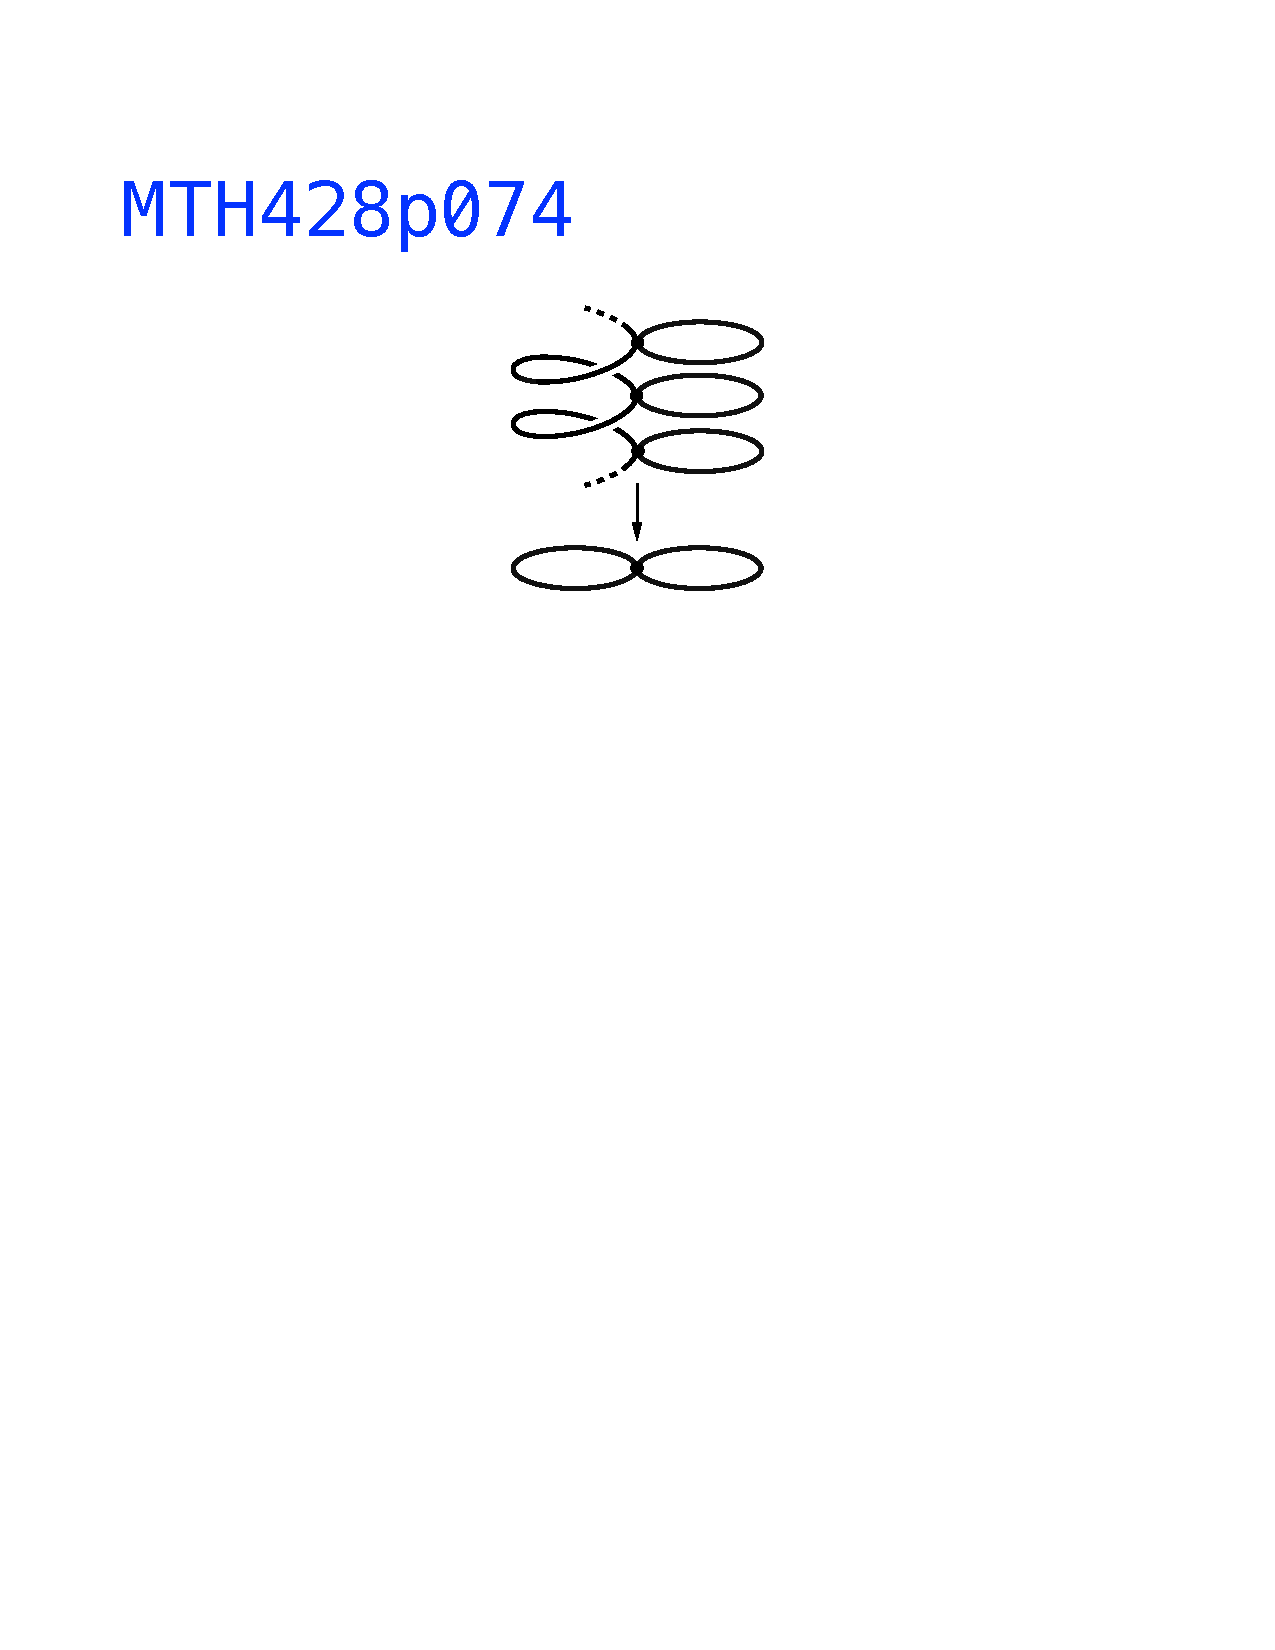
\includegraphics[width=0.93\textwidth, trim=0mm 177mm 0mm 51mm, clip]{pictures/MTH428p074.pdf}}};

%%% COORDINATE GRID
%\draw[step=0.5, help lines] (0,0) to[grid with coordinates] (15,9);
%%% 
\end{tikzpicture}
\end{equation*}

The  total space $T$ of this covering is homotopy equivalent to the space 
$\bigvee_{n\in \Z} S^{1}$, and so $\pi_{1}(T)$ is a free group on an infinite number of generators. 
By Theorem \ref{COVERINGSUBGP THM}  $\pi_{1}(T)$ can be identified with a subgroup of $\pi_{1}(S^{1}\vee S^{1})$.
\end{proof}



%%%%%%%%%%%%%%%%%%%%%%%%%%%%%%%
%  EXERCISES
%%%%%%%%%%%%%%%%%%%%%%%%%%%%%%%

\exercises

\begin{exercise}
Prove Proposition \ref{LIFTSSAMEENDS PROP}. 
\end{exercise}

\begin{exercise}
Prove Proposition \ref{REGULARCOV PROP}.
\end{exercise}

\begin{exercise}
\label{PULLBACK COVERING EXERCISE}
Let $p\colon T \to X$ be a covering and let $f\colon Y \to X$ be an arbitrary continuous function.
Let $f^{\ast}T$ be a subspace of $Y\times T$ defined by 
$$f^{\ast}T = \{(y, \ntilde x) \in Y\times T \ | \ f(y) = p(\ntilde x)\}$$ 
Let $p'\colon f^{\ast}T \to Y$ be the map given by $p'(y, \ntilde x) = y$. 

a) Show that $p'\colon f^{\ast}T \to Y$ is a covering. 

b) Assume that  $(y_{0}, \ntilde x_{0})\in f^{\ast}T$. Show that 
$p'_{\ast}(\pi_{1}(f^{\ast}T, (y_{0}, \ntilde x_{0}))) = f_{\ast}^{-1}(p_{\ast}(\pi_{1}(T, \ntilde x_{0})))$ 
where $f_{\ast}\colon \pi_{1}(Y, y_{0}) \to \pi_{1}(X, f(x_{0}))$ is the homomorphism induced by $f$.  
\end{exercise}





\begin{exercise}
 A map $p\colon E \to B$ is a fibration if it has the homotopy lifting property, i.e. if for any 
maps $F\colon X\times [0, 1] \to B$  and $\widetilde{f}\colon X\times \{0\} \to E$ satisfying 
$F|_{X\times \{0\}} = p\widetilde{f}$ there exists $\widetilde{F}\colon X\times [0, 1] \to E$ 
such that $\widetilde{F}|_{X\times \{0\}} = \widetilde{f}$ and $p\widetilde{F} = F$:

\begin{equation*}
\begin{tikzpicture}[baseline=(current  bounding  box.center)]
\matrix (m) 
[matrix of math nodes, row sep= 3em, column sep=3.5em, text height=1.5ex, text depth=0.25ex]
{
X\times \{0\}  &  E \\
X\times [0, 1] & B & \\ 
};
\path[->, thick, font=\scriptsize]
(m-1-1) 
edge node[auto] {$\widetilde{f}$} (m-1-2)
(m-1-2)
edge node[anchor=  west] {$p$} (m-2-2)
(m-2-1)
edge node[anchor= north] {$F$} (m-2-2)
; 
\path[right hook ->, thick, font=\scriptsize]
(m-1-1) 
edge node[anchor=north east] {} (m-2-1)
;
\path[->, thick, dashed, font=\scriptsize]
(m-2-1.20)
edge node[anchor= south east] {$\widetilde{F}$} (m-1-2)
;
\end{tikzpicture}
\end{equation*}
For example, any covering is a fibration. 

Let $p\colon E\to B$ be a fibration, let $b_{0}\in B$,  $F = p^{-1}(b_{0})$, and $e_{0}\in F$. 
Consider the homomorphisms 
$$\pi_{1}(F, e_{0}) \overset{i_{\ast}}{\longrightarrow} \pi_{1}(E, e_{0})  \overset{p_{\ast}}{\longrightarrow} \pi_{1}(B, b_{0})$$ 
where $i\colon F \to E$ is the inclusion map. Show that $\text{Im}(i_{\ast}) = \text{Ker}(p_{\ast})$. 

Note: if $p$ is a covering then $\pi_{1}(F, e_{0})$ is the trivial group (since $F$ is a discrete space), 
so the above formula implies that  $\text{Ker}(p_{\ast})$ is trivial. This gives another 
proof that for a covering $p$ the induced homomorphism $p_{\ast}$ is 1-1.  
\end{exercise}

\begin{exercise}
Let $p\colon E \to B$ be a fibration, let $b_{0}\in B$, and  $F = p^{-1}(b_{0})$. Show that if $B$
is a contractible space then the inclusion map $i\colon F \to E$ is a homotopy equivalence. 
\end{exercise}


\newpage
%%%%%%%%%%%%%%%%%%%%%%%%%%%%%%%
%%%%%%%%%%%%%%%%%%%%%%%%%%%%%%%
%%%
%%%  CLASSIFICATION OF COVERINGS
%%%
%%%%%%%%%%%%%%%%%%%%%%%%%%%%%%%
%%%%%%%%%%%%%%%%%%%%%%%%%%%%%%%

 %---BBLANK
\chapter[Classification of Coverings]{Classification \\ of Coverings}
 %---EBLANK 
 \chaptermark{Classification of Coverings}
\label{CLASS OF COV CHAPTER}

\thispagestyle{firststyle}


 %---BBLANK
\begin{definition}
Let $p_{1}\colon T_{1} \to X$, $p_{2}\colon T_{2}\to X$ be coverings over the same base space $X$. 
A \emph{map of coverings} is a continuous function $f\colon T_{1}\to T_{2}$ such that the following 
diagram commutes:
\begin{equation*}
\begin{tikzpicture}
\matrix (m) 
[matrix of math nodes, row sep= 2.5em, column sep=1.5em, text height=1.5ex, text depth=0.25ex]
{
T_{1} &  &  T_{2} \\
 & X & \\
};
\path[->, thick, font=\scriptsize]
(m-1-1) 
edge node[auto] {$f$} (m-1-3)
edge node[anchor = north east] {$p_{1}$} (m-2-2)
(m-1-3) 
edge node[anchor = north west] {$p_{2}$} (m-2-2)
;
\end{tikzpicture}
\end{equation*}
For a given space $X$ by $\Cov(X)$ we will denote the category whose objects are all coverings over $X$
and whose morphisms are maps of coverings. 
\end {definition}
 %---EBLANK # \vskip 30mm

In $\Cov(X)$, as in any category, we have the notion of an isomorphism of coverings. 
It is easy to check that the following holds:

 %---BBLANK
\begin{proposition}
\label{ISOSINCOVX PROP}
Let $p_{1}\colon T_{1}\to X$ and  $p_{2}\colon T_{2}\to X$ be coverings of $X$. A map of coverings 
$f\colon T_{1}\to T_{2}$ is an isomorphism in $\Cov(X)$ if and only if $f$ is a homeomorphism.
\end{proposition}

\begin{proof}
Exercise. 
\end{proof}
 %---EBLANK # \newpage


\begin{note}
If  $p_{1}\colon T_{1}\to X$ and  $p_{2}\colon T_{2}\to X$ are coverings and the spaces 
$T_{1}$ and $T_{2}$ are homeomorphic  then this does not imply that $p_{1}$ and $p_{2}$ 
are isomorphic coverings since it may happen than no homeomorphism between $T_{1}$
and $T_{2}$ is a map of coverings. For example, recall the for $n=1, 2, \dots$ we have 
an $n$-fold covering $p_{n}\colon S^{1} \to S^{1}$ given by $p_{n}(z) = z^{n}$
(where we consider $S^{1}$ as the set of unit complex numbers: $S^{1} = \{z \in \C \ | \ \norm{z} = 1 \}$). 
The total space of each of these coverings is $S^{1}$, but these coverings are non-isomorphic to one another
since an $n$-fold covering cannot be isomorphic to an $m$-fold covering for $n\neq m$ (exercise).  
\end{note}

Our goal in this chapter is to show that under some mild conditions the problem of determining if two 
coverings of $X$ are isomorphic or not can be reduced to a purely algebraic problem. Recall that a space $X$ is 
\emph{locally path connected} if for any point $x\in X$ and any open neighborhood $U\subseteq X$ of $x$
there exists an open neighborhood $V$ of $x$ such that $V\subseteq U$ and $V$ is path connected. 

 %---BBLANK
\begin{theorem}
\label{CLASSOFCOVERINGS THM}
Let $X$ be a locally path connected space, and for $i=1, 2$ let $p_{i}\colon T_{i}\to X$ be a covering 
such that $T_{i}$ is a path connected space. Let $x_{0}\in X$ and let $\ntilde{x}_{i}\in p_{i}^{-1}(x_{0})$. 
The coverings $p_{1}$ and $p_{2}$ are isomorphic if and only if the subgroup 
$p_{1\ast}(\pi_{1}(T_{1}, \ntilde{x}_{1}))\subseteq \pi_{1}(X, x_{0})$ is conjugate to 
the subgroup $p_{2\ast}(\pi_{1}(T_{2}, \ntilde{x}_{2}))$.
\end{theorem}
 %---EBLANK #\newpage

One implication of Theorem \ref{CLASSOFCOVERINGS THM} is straightforward: if the coverings $p_{1}$
and $p_{2}$ are isomorphic then we have a homeomorphism $f\colon T_{1}\to T_{2}$ that we can use 
to relate the subgroups coming from these  coverings.  The other implication is more challenging, since 
it says that based on some information about fundamental groups we can produce a map $T_{1}\to T_{2}$.
Existence of such map will follow from the next theorem which is very useful in many  applications:


 %---BBLANK
\begin{LIFTCRITTHM}
\label{LIFTINGCRIT THM}
Let $p\colon T\to X$ be a covering, let $x_{0}\in X$ and let $\ntilde{x}_{0}\in p^{-1}(x_{0})$. Assume that $Y$
is a connected and locally path connected space and let $y_{0}\in Y$.  A map $f\colon (Y, y_{0}) \to (X, x_{0})$
has a lift $\ntilde{f}\colon (Y, y_{0}) \to (T, \ntilde{x}_{0})$ if and only if 
$f_{\ast}(\pi_{1}(Y, y_{0})) \subseteq p_{\ast}(\pi_{1}(T, \ntilde{x}_{0}))$. 
\begin{equation*}
\label{LIFTINGCRIT EQ}
\tag{$\ast$}
\begin{tikzpicture}[baseline=(current  bounding  box.center)]
\matrix (m) 
[matrix of math nodes, row sep= 2.5em, column sep=3em, text height=1.5ex, text depth=0.25ex]
{
   &  T \\
Y & X & \\ 
};
\path[->, thick, font=\scriptsize]
(m-2-1) 
edge node[auto] {$\ntilde{f}$} (m-1-2)
edge node[below] {$f$} (m-2-2)
(m-1-2) 
edge node[auto] {$p$} (m-2-2)
;
\end{tikzpicture}
\end{equation*}

\end{LIFTCRITTHM}
 %---EBLANK # \newpage


\begin{note}
By Lemma \ref{COVERINGUNIQUELIFT LEMMA} if a lift $\ntilde{f}$ exists then it is unique. 
\end{note}




\begin{proof}[Proof of Theorem \ref{LIFTINGCRIT THM}]

($\Ra$) If the lift $\ntilde{f}$ exists then the diagram (\ref{LIFTINGCRIT EQ}) induces a commutative 
diagram of fundamental groups:
\begin{equation*}
\label{LIFTCRIT EQ}
\begin{tikzpicture}[baseline=(current  bounding  box.center)]
\matrix (m) 
[matrix of math nodes, row sep= 2.5em, column sep=1.5em, text height=1.5ex, text depth=0.25ex]
{
   &  \pi_{1}(T, \ntilde{x}_{0}) \\
\pi_{1}(Y, y_{0}) & \pi_{1}(X, x_{0}) & \\ 
};
\path[->, thick, font=\scriptsize]
(m-2-1) 
edge node[auto] {$\ntilde{f}_{\ast}$} (m-1-2)
edge node[below] {$f_{\ast}$} (m-2-2)
(m-1-2) 
edge node[auto] {$p_{\ast}$} (m-2-2)
;
\end{tikzpicture}
\end{equation*}
Therefore we obtain 
$$f_{\ast}(\pi_{1}(Y, y_{0})) = p_{\ast}\ntilde{f}_{\ast}(\pi_{1}(Y, y_{0})) \subseteq p_{\ast}(\pi_{1}(T, \ntilde{x}_{0}))$$


($\La$)  We will construct 
the function $\ntilde{f}\colon Y \to X$ as follows. Take $y\in Y$. Since the space $Y$ is connected and locally path 
connected thus it is path connected, and so there exists a path $\omega\colon [0, 1]\to Y$ such that 
$\omega(0) = y_{0}$ and $\omega(1)=y$. By Corollary \ref{COVERING PATH LIFT COR}  the path 
$f\omega \colon [0, 1] \to X$ admits a unique lift $\nwidetilde{f\omega} \colon [0, 1]\to T$ such that 
$\nwidetilde{f\omega}(0) = \ntilde{x}_{0}$. We set $\ntilde{f}(y) := \nwidetilde{f\omega}(1)$. 

In order to see that $\ntilde{f}$ is well defined  take $\omega'$ to be another path in $Y$
joining $y_{0}$ with $y$, and let $\nwidetilde{f\omega}'$ be the lift of $f\omega'$ satisfying 
$\nwidetilde{f\omega}'(0) = \ntilde{x}_{0}$. We need to show that 
$\nwidetilde{f\omega}(1) = \nwidetilde{f\omega}'(1)$. By Proposition \ref{LIFTSSAMEENDS PROP}
this is equivalent to showing that  $[f\omega\ast \xov{f\omega'}]\in \pi_{1}(X, x_{0})$ is 
an element of $p_{\ast}(\pi_{1}(T, \ntilde{x}_{0}))$. Notice that we have 
$$[f\omega\ast \xov{f\omega'}] = [f(\omega\ast\xov{\omega'})] = f_{\ast}([\omega\ast\xov{\omega'}])$$
where $[\omega\ast \xov{\omega'}]\in \pi_{1}(Y, y_{0})$. By assumption 
$f_{\ast}(\pi_{1}(Y, y_{0})) \subseteq p_{\ast}(\pi_{1}(T, \ntilde{x}_{0}))$, so in particular 
$ f_{\ast}([\omega\ast\xov{\omega'}]) \in p_{\ast}(\pi_{1}(T, \ntilde{x}_{0}))$. 

Directly from the construction of $\ntilde{f}$ we get that $p\ntilde{f} = f$ and that $\ntilde{f}(y_{0}) = \ntilde{x}_{0}$. 
We still need to check though that $\ntilde{f}$ is a continuous function. It will suffice to show that for any 
$y\in Y$ there is an open neighborhood $U$ of $y$ such that $\ntilde{f}|_{U}\colon U\to T$ is continuous. 
Let $V\subseteq X$ be an open neighborhood of $f(y)$ which is evenly covered, and take $U$ to be an open 
neighborhood of $y$ such that  $U\subseteq f^{-1}(V)$ and that $U$ is path connected. Such $U$ exists 
by the assumption that $Y$ is locally path connected. For any $y'\in U$ let $\tau_{y'}$ be a path in $U$ 
joining $y$ with $y'$. Also, let $\omega$ be a path in $Y$ that joins $y_{0}$ with $y$. Notice that 
$\omega\ast\tau_{y'}$ joins $y_{0}$ and $y'$, so $\ntilde{f}(y') = \nwidetilde{\omega\ast \tau}_{y'}(1)$
where $\nwidetilde{\omega\ast \tau}_{y'}$ is the lift of $\omega\ast\tau_{y'}$ that starts at $\ntilde{x}_{0}$. 
On the other hand $\nwidetilde{\omega\ast \tau}_{y'} = \nwidetilde{\omega}\ast \nwidetilde{\tau}_{y'}$
where $\nwidetilde{\omega}$ is the lift of $\omega$ that starts at $\ntilde{x}_{0}$, and 
$\nwidetilde{\tau}_{y}$ is the lift of $\tau_{y}$ that starts at $\nwidetilde{\omega}(1) = \ntilde{f}(y)$. 
In effect we obtain that $\ntilde{f}(y') = \nwidetilde{\tau}_{y'}(1)$ for all $y'\in U$. Let $\nwidetilde{V}$
be the slice over $V$ such that $\ntilde{y}\in V$. The map $p|_{\nwidetilde{V}}\colon \nwidetilde{V} \to V$
is a homeomorphism. Notice that for any $y'\in U$ we have 
$\nwidetilde{\tau}_{y'} = (p|_{\nwidetilde{V}})^{-1}f\tau_{y'}$. This gives:
$$\ntilde{f}(y') = \nwidetilde{\tau}_{y'}(1) =  (p|_{\nwidetilde{V}})^{-1}f\tau_{y'}(1) =  (p|_{\nwidetilde{V}})^{-1}f(y')$$
In other words we obtain $\ntilde{f}|_{U} = (p|_{\nwidetilde{V}})^{-1}f$, which means that   
$\ntilde{f}|_{U}$ is a continuous function.  
\begin{equation*}
\begin{tikzpicture}

\node[anchor=south west,inner sep=0] at (0,0) 
{{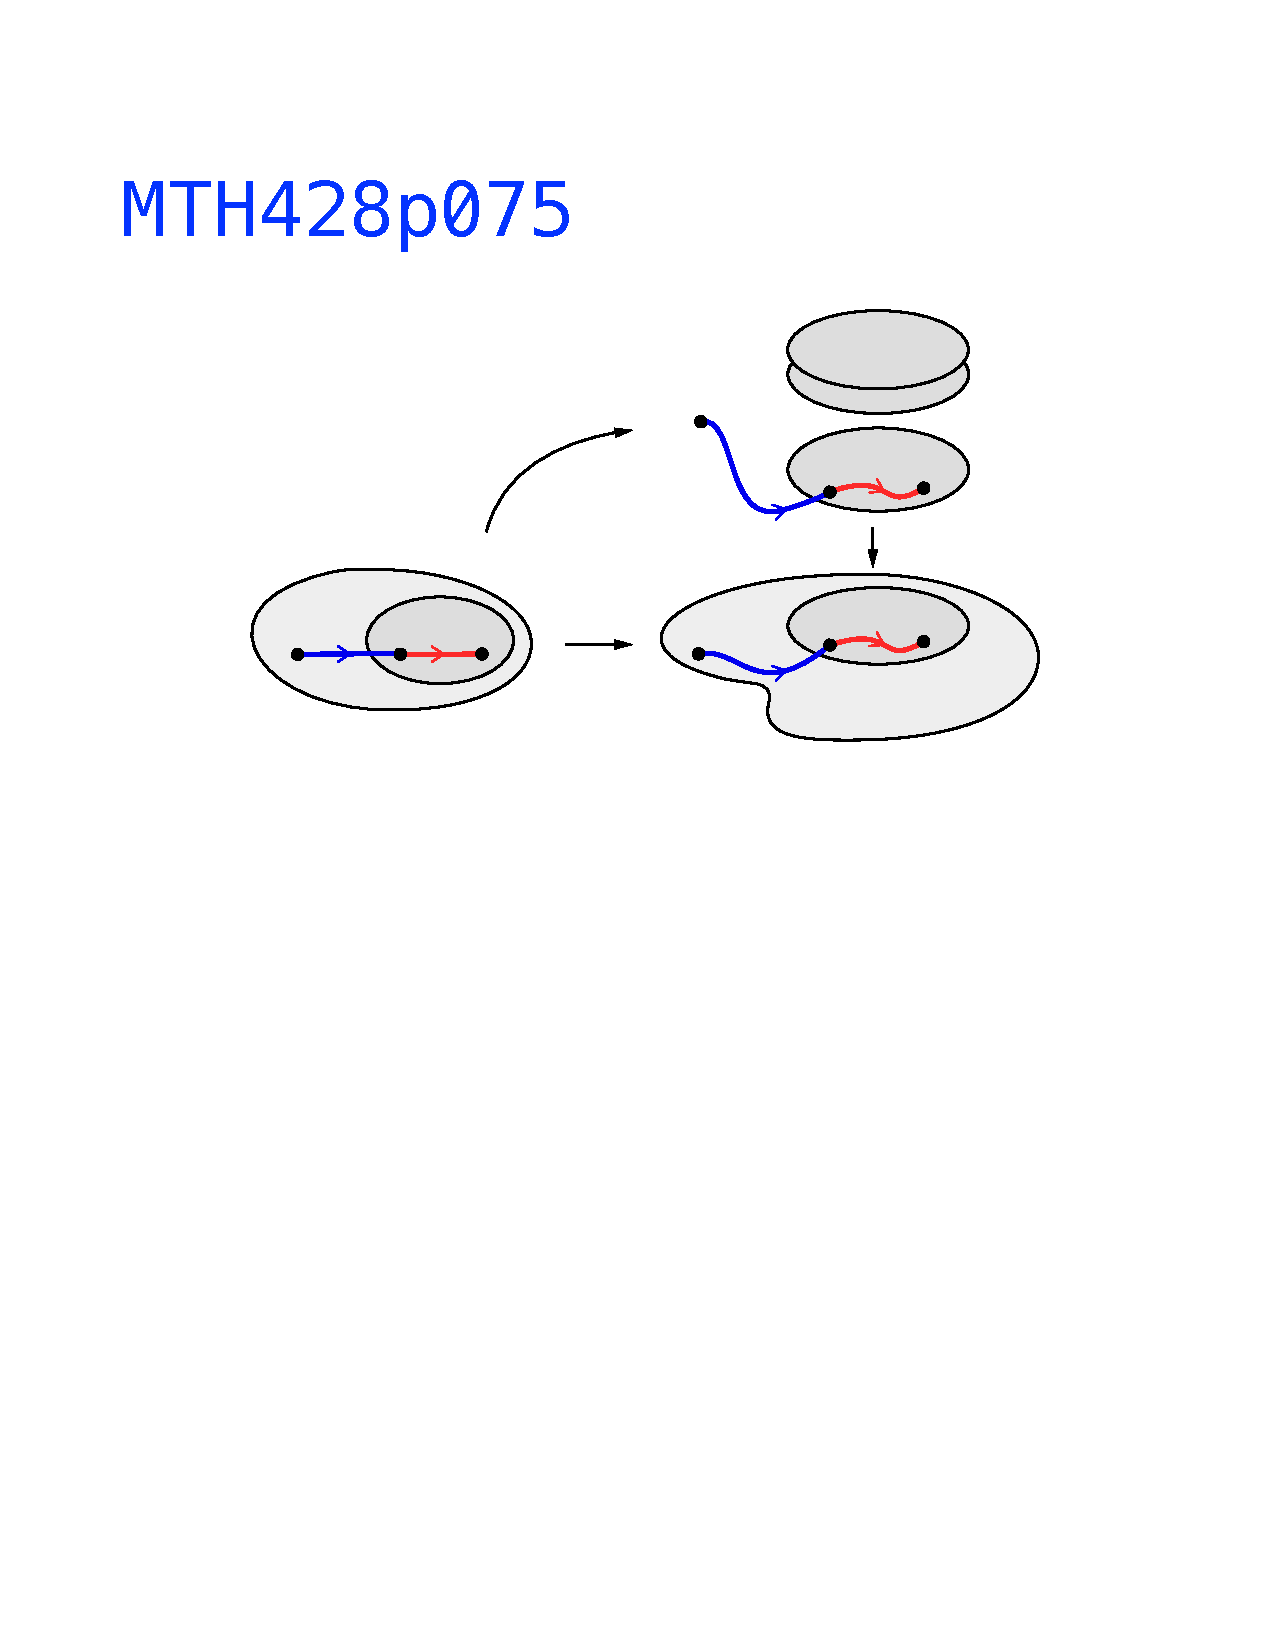
\includegraphics[width=\textwidth, trim=0mm 152mm 0mm 52mm, clip]{pictures/MTH428p075.pdf}}};

%%% COORDINATE GRID
%\draw[step=0.5, help lines] (0,0) to[grid with coordinates] (15,9);
%%% 
\node[anchor= base]  at (4.0 , 1.5){\small  $y_{0}$};
\node[anchor= base]  at (5.25 , 1.5){\small  $y$};
\node[anchor= base]  at (6.33 , 1.5){\small  $y'$};
\node[anchor= base]  at (9.15 , 1.5){\small  $x_{0}$};
\node[anchor= base]  at (10.8 , 	1.65){\small  $f(y)$};
\node[anchor= base]  at (12.0 , 	1.65){\small  $f(y')$};
\node[anchor= base]  at (10.8 , 	3.62){\small  $\ntilde{f}(y)$};
\node[anchor= base]  at (12.0 , 	3.65){\small  $\ntilde{f}(y')$};
\node[anchor= base]  at (9.15 , 4.5){\small  $\ntilde{x}_{0}$};
\node[anchor= base west]  at (12.55 , 3.55){\small $\nwidetilde{V}$};
\node[anchor= base west]  at (12.55 , 1.52){\small $V$};
\node[anchor= base]  at (11.55, 2.7){\small  $p$};
\node[anchor= base]  at (7.75, 1.5){\small  $f$};
\node[anchor= base]  at (6.83, 3.8){\small  $\ntilde{f}$};
\end{tikzpicture}
\end{equation*}


\end{proof}











\begin{proof}[Proof of Theorem \ref{CLASSOFCOVERINGS THM}]
($\Ra$) Assume that we have an isomorphism of coverings:
\begin{center}
\begin{tikzpicture}
\matrix (m) 
[matrix of math nodes, row sep= 2.5em, column sep=1.5em, text height=1.5ex, text depth=0.25ex]
{
T_{1} &  &  T_{2} \\
 & X & \\
};
\path[->, thick, font=\scriptsize]
(m-1-1) 
edge node[auto] {$f$}  node[below] {$\cong$} (m-1-3)
edge node[anchor = north east] {$p_{1}$} (m-2-2)
(m-1-3) 
edge node[anchor = north west] {$p_{2}$} (m-2-2)
;
\end{tikzpicture}
\end{center}
This gives a commutative diagram of fundamental groups:
\begin{center}
\begin{tikzpicture}
\matrix (m) 
[matrix of math nodes, row sep= 2.5em, column sep=-1em, text height=1.5ex, text depth=0.25ex]
{
\pi_{1}(T_{1}, \ntilde{x}_{1}) &  &  \pi_{1}(T_{2}, f(\ntilde{x}_{1})) \\
 & \pi_{1}(X, x_{0}) & \\
};
\path[->, thick, font=\scriptsize]
(m-1-1) 
edge node[auto] {$f_{\ast}$}  node[below] {$\cong$} (m-1-3)
edge node[anchor = north east] {$p_{1\ast}$} (m-2-2)
(m-1-3) 
edge node[anchor = north west] {$p_{2\ast}$} (m-2-2)
;
\end{tikzpicture}
\end{center}
Since $f_{\ast}$ is an isomorphism we obtain that 
$p_{1\ast}(\pi_{1}(T_{1}, \ntilde{x}_{1})) = p_{2\ast}(\pi_{1}(T_{2}, f(\ntilde{x}_{1})))$. 
It remains to notice that since $f(\ntilde{x}_{1}), \ntilde{x}_{2} \in p_{2}^{-1}(x_{0})$ thus
by Proposition  \ref{COVCONJUGSUBGPS PROP} the subgroups $p_{2\ast}(\pi_{1}(T_{2}, f(\ntilde{x}_{1})))$
and $p_{2\ast}(\pi_{1}(T_{2}, \ntilde{x}_{2}))$ are conjugate in $\pi_{1}(X, x_{0})$. 

($\La$) Assume that $p_{1\ast}(\pi_{1}(T_{1}, \ntilde{x}_{1}))$ and $p_{2\ast}(\pi_{1}(T_{2}, \ntilde{x}_{2}))$ are 
conjugate subgroups of $\pi_{1}(X, x_{0})$. By Proposition \ref{COVCONJUGSUBGPS PROP} we can find 
$\ntilde{x}'_{2}\in p_{2}^{-1}(x_{0})$ such that 
$p_{1\ast}(\pi_{1}(T_{1}, \ntilde{x}_{1})) = p_{2\ast}(\pi_{1}(T_{2}, \ntilde{x}'_{2}))$. Since the space 
$X$ is locally path connected, thus so are $T_{1}$ and $T_{2}$.  By the Lifting Criterion 
\ref{LIFTINGCRIT THM} there exists maps $\nwidetilde{p}_{1}\colon (T_{1}, \ntilde{x}_{1}) \to (T_{2}, \ntilde{x}'_{2})$
and $\nwidetilde{p}_{2}\colon (T_{2}, \ntilde{x}'_{2}) \to (T_{1}, \ntilde{x}_{1})$ such that the following 
diagrams commute:
\begin{equation*}
\begin{tikzpicture}[baseline=(current  bounding  box.center)]
\matrix (m) 
[matrix of math nodes, row sep= 2.5em, column sep=3em, text height=1.5ex, text depth=0.25ex]
{
   &  T_{2} \\
T_{1} & X & \\ 
};
\path[->, thick, font=\scriptsize]
(m-2-1) 
edge node[auto] {$\nwidetilde{p}_{1}$} (m-1-2)
edge node[below] {$p_{1}$} (m-2-2)
(m-1-2) 
edge node[auto] {$p_{2}$} (m-2-2)
;
\begin{scope}[xshift = 35mm]
\matrix (m) 
[matrix of math nodes, row sep= 2.5em, column sep=3em, text height=1.5ex, text depth=0.25ex]
{
   &  T_{1} \\
T_{2} & X & \\ 
};
\path[->, thick, font=\scriptsize]
(m-2-1) 
edge node[auto] {$\nwidetilde{p}_{2}$} (m-1-2)
edge node[below] {$p_{2}$} (m-2-2)
(m-1-2) 
edge node[auto] {$p_{1}$} (m-2-2)
;
\end{scope}
\end{tikzpicture}
\end{equation*}
We will show that $\nwidetilde{p}_{1}$ and $\nwidetilde{p}_{2}$ are inverse isomorphisms of coverings.
Notice that both $\nwidetilde{p}_{2}\nwidetilde{p}_{1}$ the identity map $\id_{T_{1}}$ fit into the commutative diagram
\begin{equation*}
\begin{tikzpicture}
\matrix (m) 
[matrix of math nodes, row sep= 3em, column sep=4.5em, text height=1.5ex, text depth=0.25ex]
{
   &  T_{1} \\
T_{1} & X & \\ 
};
\path[->, thick, font=\scriptsize]
(m-1-2)
edge node[anchor=  west] {$p_{1}$} (m-2-2)
(m-2-1)
edge node[anchor= north] {$p_{1}$} (m-2-2)
; 
\path[->, thick, transform canvas = {xshift = -0.3ex, yshift = 0.3ex}, font=\scriptsize]
(m-2-1.50)
edge node[anchor= south east] {$\nwidetilde{p}_{2}\nwidetilde{p}_{1}$} (m-1-2.200)
;
\path[->, thick, transform canvas = {xshift = 0.3ex, yshift = -0.3ex}, font=\scriptsize]
(m-2-1.50)
edge node[anchor= north west] {$\id_{T_{1}}$} (m-1-2.200)
;
\end{tikzpicture}
\end{equation*}
Moreover $\nwidetilde{p}_{2}\nwidetilde{p}_{1}(\ntilde{x}_{1}) = \ntilde{x}_{1} = \id_{T_{1}}(\ntilde{x}_{1})$. 
By Lemma \ref{COVERINGUNIQUELIFT LEMMA} this implies that 
$\nwidetilde{p}_{2}\nwidetilde{p}_{1} = \id_{T_{1}}$. An analogous argument shows that 
 $\nwidetilde{p}_{1}\nwidetilde{p}_{2} = \id_{T_{2}}$.
\end{proof}

\begin{note}
Theorem  \ref{CLASSOFCOVERINGS THM} gives  a correspondence between isomorphism classes of 
path connected coverings over $X$ and conjugacy classes of subgroups of $\pi_{1}(X, x_{0})$. There is also 
a variant of of this correspondence that takes values in the set of subgroups of $\pi_{1}(X, x_{0})$ (rather that 
conjugacy classes of subgroups). Namely, let $(X, x_{0})$ be a pointed space. A pointed covering is a 
basepoint preserving map $p\colon (T, \ntilde{x}_{0}) \to (X, x_{0})$ where $p$ is a covering. If 
$p_{1}\colon (T_{1}, \ntilde{x}_{1}) \to (X, x_{0})$ and $p_{2}\colon  (T_{1}, \ntilde{x}_{2}) \to (X, x_{0})$
are pointed coverings then a map of pointed covering is a function 
$f\colon (T_{1}, \ntilde{x}_{1}) \to (T_{2}, \ntilde{x}_{2})$ such that $p_{2}f = p_{1}$. Pointed coverings of 
$(X, x_{0})$ and their maps form a category $\Cov_{\ast}(X, x_{0})$. Modifying the proof of 
Theorem \ref{CLASSOFCOVERINGS THM} we obtain:
\end{note}

 %---BBLANK
\begin{theorem}
\label{CLASSOFPOINTEDCOVERINGS THM} 
Let $(X, x_{0})$ be a locally path connected space, and for $i=1, 2$ let 
$p_{i}\colon (T_{i}, \ntilde{x}_{i}) \to (X, x_{0})$ be a pointed covering 
such that $T_{i}$ is a path connected space. The coverings $p_{1}$ and $p_{2}$ are isomorphic 
in the category $\Cov_{\ast}(X, x_{0})$ if and only if
$p_{1\ast}(\pi_{1}(T_{1}, \ntilde{x}_{1})) = p_{2\ast}(\pi_{1}(T_{2}, \ntilde{x}_{2}))$.
\end{theorem}

\begin{proof}
Exercise. 
\end{proof}
 %---EBLANK # \newpage

%%%%%%%%%%%%%%%%%%%%%%%%%%%%%%%
%  EXERCISES
%%%%%%%%%%%%%%%%%%%%%%%%%%%%%%%

\exercises

\begin{exercise}
Prove Proposition \ref{ISOSINCOVX PROP}.
\end{exercise}


\begin{exercise}
\label{COV MAPS ONTO EXERCISE}
Consider a commutative diagram 
\begin{equation*}
\begin{tikzpicture}
\matrix (m) 
[matrix of math nodes, row sep= 2.5em, column sep=1.5em, text height=1.5ex, text depth=0.25ex]
{
T_{1} &  &  T_{2} \\
 & X & \\
};
\path[->, thick, font=\scriptsize]
(m-1-1) 
edge node[auto] {$f$} (m-1-3)
edge node[anchor = north east] {$p_{1}$} (m-2-2)
(m-1-3) 
edge node[anchor = north west] {$p_{2}$} (m-2-2)
;
\end{tikzpicture}
\end{equation*}
where $p_{1}$, $p_{2}$ are coverings and $T_{1}$, $T_{2}$ are path connected spaces. Show that 
$f$ is onto. 
\end{exercise}



\begin{exercise}
Assume that we have a map of coverings
\begin{equation*}
\begin{tikzpicture}
\matrix (m) 
[matrix of math nodes, row sep= 2.5em, column sep=1.5em, text height=1.5ex, text depth=0.25ex]
{
T_{1} &  &  T_{2} \\
 & X & \\
};
\path[->, thick, font=\scriptsize]
(m-1-1) 
edge node[auto] {$f$} (m-1-3)
edge node[anchor = north east] {$p_{1}$} (m-2-2)
(m-1-3) 
edge node[anchor = north west] {$p_{2}$} (m-2-2)
;
\end{tikzpicture}
\end{equation*}
where $T_{1}$, $T_{2}$ are path connected spaces. Assume also that for some $x_{0}\in X$ the map 
$$f|_{p^{-1}(x_{0})}\colon p_{1}^{-1}(x_{0}) \to p_{2}^{-1}(x_{0})$$ 
is 1-1. Show that $f\colon T_{1}\to T_{2}$ is 1-1. 
\end{exercise}





\begin{exercise}
Let $X$ be a locally path connected space, and  let $p \colon T\to X$ be a covering such that 
$T$ is a path connected space and $\pi_{1}(T)$ is a finite group. Show that any map of coverings 

\begin{equation*}
\begin{tikzpicture}
\matrix (m) 
[matrix of math nodes, row sep= 2.5em, column sep=1.5em, text height=1.5ex, text depth=0.25ex]
{
T &  &  T \\
 & X & \\
};
\path[->, thick, font=\scriptsize]
(m-1-1) 
edge node[anchor=south] {$f$} (m-1-3)
edge node[anchor = north east] {$p$} (m-2-2)
(m-1-3) 
edge node[anchor = north west] {$p$} (m-2-2)
;
\end{tikzpicture}
\end{equation*}
is an isomorphism. 
\end{exercise}



\begin{exercise}
Recall that the $n$-th homotopy group of a pointed space $(X, x_{0})$
is the group whose elements are homotopy classes of basepoint preserving 
maps $(S^{n}, s_{0}) \to (X, x_{0})$. Let $x_{0}\in S^{1}$. Show that 
$\pi_{n}(S^{1}, x_{0})$ is a trival group for $n>1$. 
\end{exercise}

\begin{exercise}
Let $X$ be a  locally path connected space, $x_{0}\in X$, and let $p\colon T \to X$ 
be a covering with a path connected space $T$. Show that the following conditions are equivalent:

\begin{itemize}
\item[(i)] The covering $p\colon T \to X$ is regular
\item[(ii)] For any points $\tilde{x}_{1}, \tilde{x}_{2}\in p^{-1}(x_{0})$ 
there exists a map of coverings 
\begin{equation*}
\begin{tikzpicture}
\matrix (m) 
[matrix of math nodes, row sep= 2.5em, column sep=1.5em, text height=1.5ex, text depth=0.25ex]
{
T &  &  T \\
 & X & \\
};
\path[->, thick, font=\scriptsize]
(m-1-1) 
edge node[auto] {$f$} (m-1-3)
edge node[anchor = north east, pos = 0.4] {$p$} (m-2-2)
(m-1-3) 
edge node[anchor = north west,  pos = 0.4] {$p$} (m-2-2)
;
\end{tikzpicture}
\end{equation*}
such that $f(\tilde x_{1}) = \tilde x_{2}$. 

\end{itemize}
\end{exercise}





\begin{exercise}
Let $p\colon T\to X$ be a covering such that $T$, $X$ are connected and locally path connected 
spaces. Assume that there exists a function $s\colon X\to T$ such that $ps = \id_{X}$. Show that 
$T$ is homeomorphic to $X$. 
\end{exercise}




\begin{exercise}
Let  $p\colon T \to X$ be a covering such that $X$ is locally path connected, and  $T$ is path connected. 
Given maps $f, g \colon Y \to X$ let $p'\colon f^{\ast}T \to Y$ and  $p''\colon g^{\ast}T \to Y$ be the coverings of  $Y$ 
obtained from $p$ using $f$ and $g$, respectively,  as in Exercise \ref{PULLBACK COVERING EXERCISE}. 
Show that if $f \simeq g$ then $p'$ and $p''$ are isomorphic coverings. 
\end{exercise}



\newpage
%%%%%%%%%%%%%%%%%%%%%%%%%%%%%%%
%%%%%%%%%%%%%%%%%%%%%%%%%%%%%%%
%%%
%%%  FROM SUBGROUPS TO COVERINGS
%%%
%%%%%%%%%%%%%%%%%%%%%%%%%%%%%%%
%%%%%%%%%%%%%%%%%%%%%%%%%%%%%%%

 %---BBLANK
\chapter[From Subgroups to Coverings]{From Subgroups \\to Coverings}
 %---EBLANK
\chaptermark{From Subgroups to Coverings}

\label{FROM SUBGP TO COV CHAPTER}


In the last chapter we have seen that if $X$ is a locally path connected space and $x_{0}\in X$
then there are 1-1 functions: 

 %---BBLANK # \vskip 30mm 
\begin{center}
\begin{tabular}{ccc}
$
\begin{pmatrix}
\text{\ \ isomorphism classes\ \ } \\[1mm]
\text{of path connected} \\[1mm]
\text{coverings of $X$} \\
\end{pmatrix}
$
& 
$\overset{\Omega}{\lra}$
&
$ 
\begin{pmatrix}
\text{conjugacy classes} \\[1mm]
\text{of subgroups} \\[1mm]
\text{of $\pi_{1}(X, x_{0})$} \\
\end{pmatrix}
$
\\
\\
$
\begin{pmatrix}
\text{isomorphism classes of} \\[1mm]
\text{pointed path connected} \\[1mm]
\text{coverings of $(X, x_{0})$} \\
\end{pmatrix}
$
& $\overset{\Omega}\lra$ & 
$
\begin{pmatrix}
\text{\ \ \ \  subgroups  \ \ \ \  } \\[1mm]
\text{of} \\[1mm]
\text{$\pi_{1}(X, x_{0})$} \\
\end{pmatrix}
$
\end{tabular}
\end{center}
 %---EBLANK # \newpage
In both cases the function $\Omega$ associates to a covering $p\colon T\to X$ with $\ntilde{x}_{0}\in p^{-1}(x_{0})$
the (conjugacy class of) subgroup $p_{\ast}(\pi_{1}(T, \ntilde{x}_{0}))\subseteq \pi_{1}(X, x_{0})$. The natural question 
is for which subgroups $H\subseteq \pi_{1}(X, x_{0})$ there exists a covering $p \colon T\to X$ such that 
$\Omega(p) = H$. Our goal here will be to prove that under some assumptions on $X$ such covering $p$ exists  for any subgroup $H$, and so the maps $\Omega$ given above are bijections. As the first step we will show that 
$\Omega$ is a bijection provided that there exists a covering of $X$ corresponding to the trivial subgroup of $\pi_{1}(X, x_{0})$. 

 %---BBLANK
\begin{definition}
Let $X$ be a locally path connected space. A \emph{universal covering} of $X$ is a covering 
$\tilde{p}\colon \widetilde{X} \to X$ such that $\widetilde X$ is a simply connected space. 
\end{definition}
 %---EBLANK

Directly from the Lifting Criterion \ref{LIFTINGCRIT THM} we obtain: 

 %---BBLANK # \vskip 40mm
\begin{proposition}
\label{UNIV COVER ONTO ANY COVER PROP}
Let $X$ be a locally path connected space and  $\tilde{p}\colon \widetilde{X} \to X$ be a universal covering of $X$.
For any covering  $q\colon T \to X$ there exists a map of coverings: 

\begin{equation*}
\begin{tikzpicture}
\matrix (m) 
[matrix of math nodes, row sep= 2.5em, column sep=1.5em, text height=1.5ex, text depth=0.25ex]
{
\widetilde{X} &  &  T \\
 & X & \\
};
\path[->, thick, font=\scriptsize]
(m-1-1) 
edge node[auto] {$f$} (m-1-3)
edge node[anchor = north east] {$\tilde{p}$} (m-2-2)
(m-1-3) 
edge node[anchor = north west] {$q$} (m-2-2)
;
\end{tikzpicture}
\end{equation*}
\end{proposition}
 %---EBLANK


Notice that by Exercise \ref{COV MAPS ONTO EXERCISE} if $T$ is path connected then 
the map $f$ in Proposition \ref{UNIV COVER ONTO ANY COVER PROP} is onto. This suggests 
that if $X$ has a universal covering then any path connected covering of $X$ may be obtained 
as a quotient space of the universal covering space $\widetilde X$. This is the main idea in the 
proof of the following fact:


 %---BBLANK # \newpage
\begin{theorem}
\label{UNIVCOVERGIVESALL THM}
Let $X$ be a locally path connected space and let $x_{0}\in X$. If there exists a universal covering 
$\tilde{p}\colon \nwidetilde{X}\to X$ then for each subgroup $H\subseteq \pi_{1}(X, x_{0})$ 
there exists a covering $p_{H}\colon T_{H} \to X$ and $\ntilde{x}_{H}\in p_{H}^{-1}(x_{0})$ such that 
$p_{H\ast}(\pi_{1}(T_{H}, \ntilde{x}_{H})) = H$. 
\end{theorem}
 %---EBLANK # \newpage

\begin{proof}
Let $H\subseteq \pi_{1}(X, x_{0})$ be a subgroup. Let $\tilde{p}\colon \nwidetilde{X}\to X$ be a universal covering 
of $X$ and let $y_{0}\in \tilde{p}^{-1}(x_{0})$. 
For each point $y\in \nwidetilde{X}$ let  $\tau_{y}$ be a path in $\nwidetilde{X}$ joining $y_{0}$ with $y$. 
Notice that if $\tilde p(y)  = \tilde p(y')$ then the path $\tilde p\tau_{y} \ast  \tilde p \overline{\tau_{y'}}$ is 
loop in $X$ based at $x_{0}$. Notice also that the homotopy class of this loop does not depend on the 
choice of paths $\tau_{y}$ and $\tau_{y'}$. Indeed, if $\sigma_{y}$ and $\sigma_{y'}$ are some other paths 
in $\widetilde X$ joining $y_{0}$ with, respectively, $y$ and $y'$ then, since $\nwidetilde X$ is simply connected, by 
Proposition \ref{SIMPLY CONN PROP} we obtain $\tau_{y}\simeq \sigma_{y}$ and $\tau_{y'}\simeq \sigma_{y'}$
which gives a homotopy 
$\tilde p\tau_{y} \ast  \tilde p \overline{\tau_{y'}} \simeq \tilde p\sigma_{y} \ast  \tilde p \overline{\sigma_{y'}}$.

Define a relation $\sim$ on $\nwidetilde X$ such that $y\sim y'$ if 
\benu
\item[(i)] $\tilde p (y) = \tilde p (y')$
\item[(ii)] $[\tilde p\tau_{y} \ast  \tilde p \overline{\tau_{y'}}] \in H$
\eenu 

One can check that $\sim$ is an equivalence relation on $\nwidetilde X$ (exercise). 
Denote the quotient space by $X_{H}$ and let $q\colon \nwidetilde X \to X_{H}$ be the quotient map.  
We get a commutative diagram  
\begin{equation*}
\begin{tikzpicture}
\matrix (m) 
[matrix of math nodes, row sep= 2.5em, column sep=1.5em, text height=1.5ex, text depth=0.25ex]
{
\nwidetilde{X} &  &  X_{H} \\
 & X & \\
};
\path[->, thick, font=\scriptsize]
(m-1-1) 
edge node[auto] {$q$} (m-1-3)
edge node[anchor = north east] {$\tilde{p}$} (m-2-2)
(m-1-3) 
edge node[anchor = north west] {$p_{H}$} (m-2-2)
;
\end{tikzpicture}
\end{equation*}
where $p_{H}$ is given by $p_{H}([y]) = \tilde p(y)$. 
We will prove that  $p_{H}\colon X_{H} \to X$ is a covering. Let $x\in X$ and let $U\subseteq X$  be 
an open neighborhood of $x$ which is $U$ is path connected and evenly covered by $\tilde p$. 
Such $U$ exists by the assumption that $X$ is locally path connected. We will show that $U$ is evenly 
covered by $p_{H}$. We have  $\tilde p^{-1}(U) = \bigcup_{i\in I} \nwidetilde U_{i} $ where $\{\nwidetilde U_{i}\}_{i\in I}$
is the set of all distinct slices of $\tilde p$ over $U$. Notice that if $y, y'$ are points in the same slice 
$\nwidetilde U_{i}$ and $y\neq y'$ then $y\not\sim y'$ since $\tilde p(y)\neq \tilde p(y')$. 
On the other hand we claim that the following holds:

\emph{Claim.} If $\nwidetilde U_{i}$, $\nwidetilde U_{j}$ are two slices, and there exist points 
$y_{i}\in \nwidetilde U_{i}$, $y_{j}\in \nwidetilde U_{j}$ such that $y_{i}\sim y_{j}$ then for every  
$y'_{i}\in \nwidetilde U_{i}$, $y'_{j}\in \nwidetilde U_{j}$ such that $\tilde p(y'_{i}) = \tilde p(y'_{j})$
we have $y'_{i} \sim y'_{j}$. 

To see this denote $x = \tilde p(y_{i}) = \tilde p(y_{j})$ and $x' = \tilde p(y'_{i}) = \tilde p(y'_{j})$. Since 
$x, x'\in U$ and $U$ is path connected we can find a path $\sigma$ in $U$ such that  $\sigma(0) = x$
and $\sigma(1) =  x'$. 
Denote by $\nwidetilde \sigma_{i}$ and $\nwidetilde \sigma_{j}$ the lifts of $\sigma$ to, respectively 
$\nwidetilde U_{i}$ and $\nwidetilde U_{j}$. Notice that $\nwidetilde \sigma_{i}(0) = y_{i}$, 
$\nwidetilde \sigma_{i}(1) = y'_{i}$, and likewise $\nwidetilde \sigma_{j}(0) = y_{j}$, 
$\nwidetilde \sigma_{j}(1) = y'_{j}$. Denote also by $\tau_{y_{i}}$, $\tau_{y_{j}}$ paths in $\nwidetilde X$
that connect the point $y_{0}$ to, respectively $y_{i}$ and $y_{j}$:
\begin{equation*}
\begin{tikzpicture}

\node[anchor=south west,inner sep=0] at (0,0) 
{{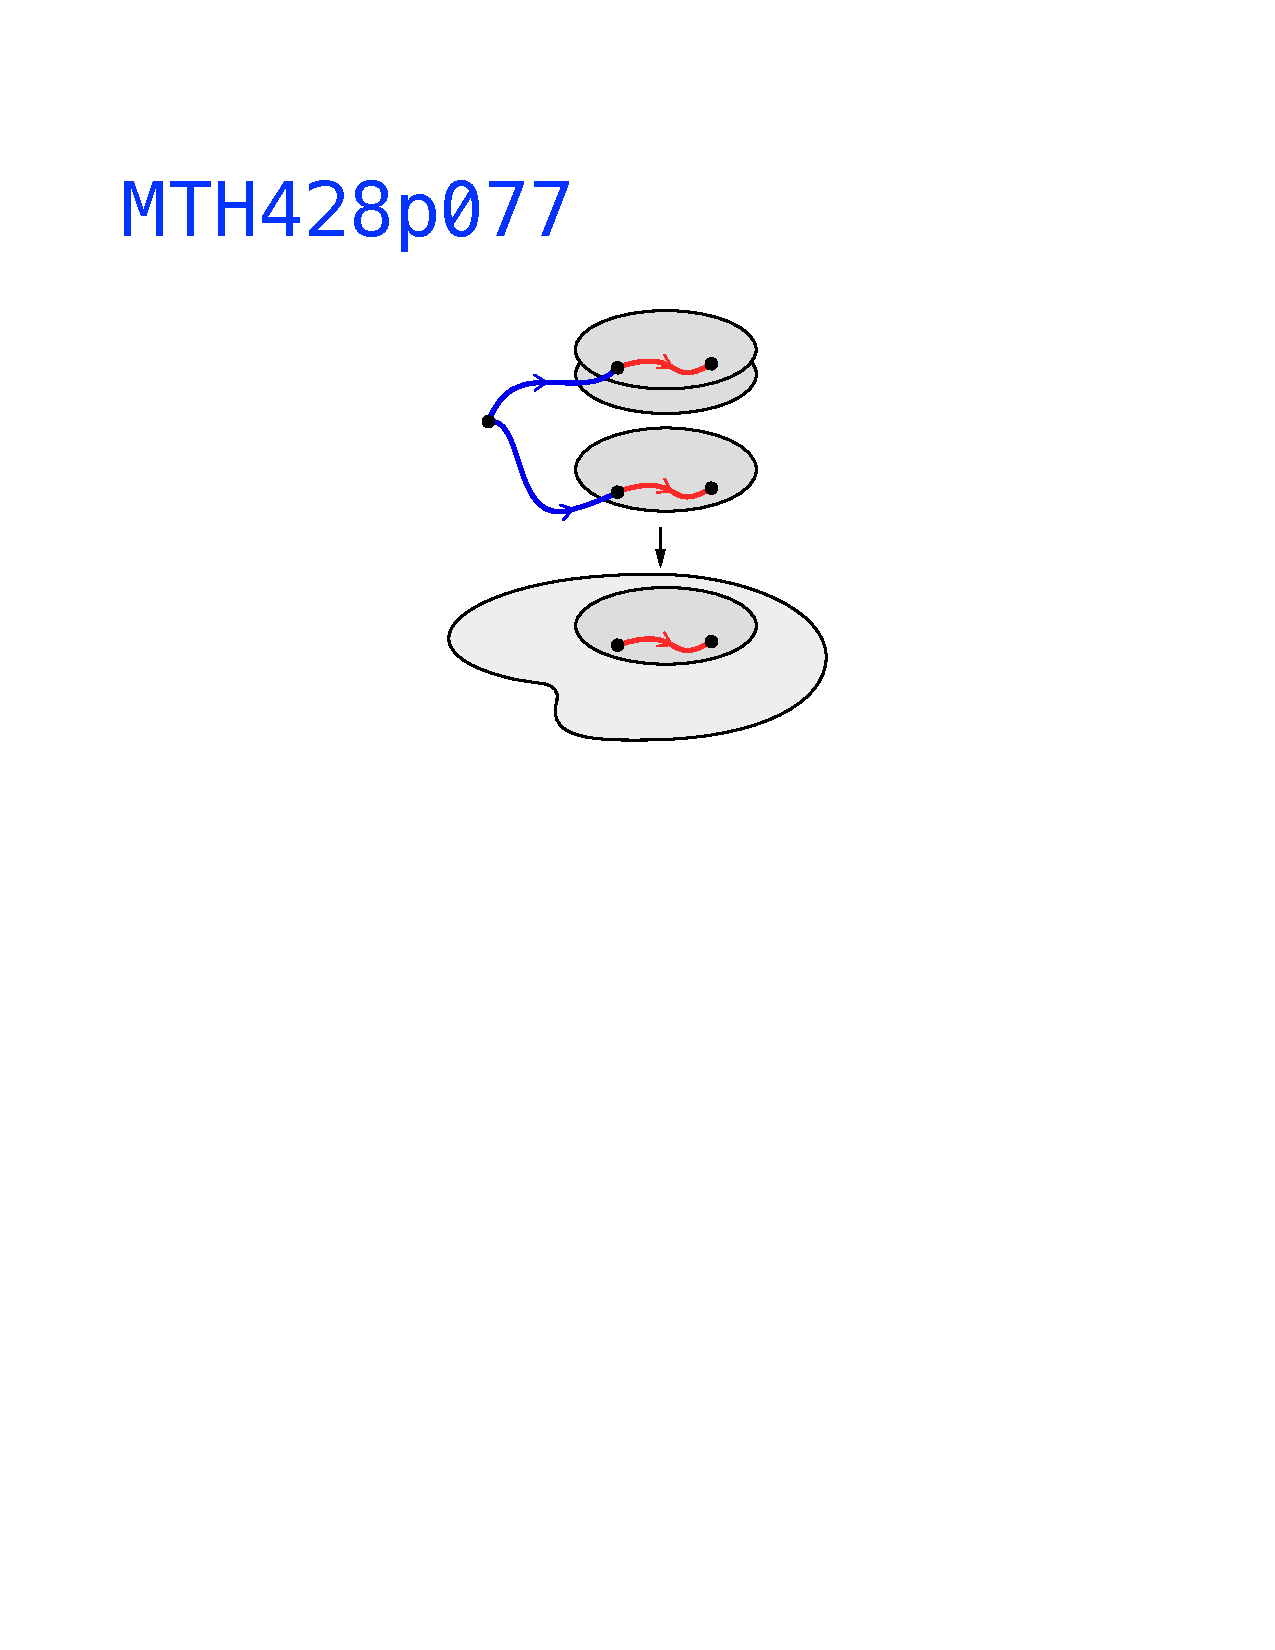
\includegraphics[width=\textwidth, trim=0mm 152mm 0mm 52mm, clip]{pictures/MTH428p077.pdf}}};

%%% COORDINATE GRID
%\draw[step=0.5, help lines] (0,0) to[grid with coordinates] (15,9);
%%% 
\node[anchor= base]  at (8.03, 1.55){\small  $x$};
\node[anchor= base]  at (9.3 , 1.6){\small  $x'$};
\node[anchor= base]  at (8.03, 3.65){\small  $y_{i}$};
\node[anchor= base]  at (9.3 , 3.7){\small  $y_{i}'$};
\node[anchor= base]  at (8.03, 5.25){\small  $y_{j}$};
\node[anchor= base]  at (9.3 , 5.3){\small  $y_{j}'$};
\node[anchor= base]  at (6.0 , 4.2){\small  $y_{0}$};
\node[anchor= base, color = red]  at (8.6 , 1.65){\small  $\sigma$};
\node[anchor= base, color = red]  at (8.6 , 3.65){\small  $\nwidetilde\sigma_{i}$};
\node[anchor= base, color = red]  at (8.6 , 5.3){\small  $\nwidetilde\sigma_{j}$};
\node[anchor= base west]  at (9.8 , 3.55){\small $\nwidetilde{U}_{i}$};
\node[anchor= base west]  at (9.8 , 5.2){\small $\nwidetilde{U}_{j}$};
\node[anchor= base west]  at (9.8 , 1.52){\small $U$};
\node[anchor= base, color = myblue]  at (7.35 , 2.7){\small  $\tau_{y_{i}}$};
\node[anchor= base, color = myblue]  at (6.95 , 5.1){\small  $\tau_{y_{j}}$};
\node[anchor= base]  at (8.8, 2.7){\small  $\tilde p$};

\end{tikzpicture}
\end{equation*}
By the definition of the  relation $\sim$ in order to show that $y_{i}' \sim y_{j}'$ we only need 
to verify that 
$[\tilde p(\tau_{y_{i}}\ast\nwidetilde\sigma_{i}) \ast \tilde p\overline{(\tau_{y_{j}}\ast\nwidetilde\sigma_{j})}]\in H$. 
This holds since
$$[\tilde p(\tau_{y_{i}}\ast\nwidetilde\sigma_{i}) \ast \tilde p\overline{(\tau_{y_{j}}\ast\nwidetilde\sigma_{j})}] = 
[\tilde p\tau_{y_{i}}\ast \sigma \ast \overline\sigma\ast \tilde p\overline{\tau_{y_{j}}}] = 
[\tilde p\tau_{y_{i}}\ast \tilde p\overline{\tau_{y_{j}}}]$$
and  $[\tilde p\tau_{y_{i}}\ast \tilde p\overline{\tau_{y_{j}}}] \in H$, since by assumption $y_{i}\sim y_{j}$. 

The statement of the claim implies that for any slice $\nwidetilde U_{i}$ the set $q^{-1}(q(\nwidetilde U_{i}))$ 
is a union of some number of slices of $\tilde p$ over $U$, and so it is an open set in $\nwidetilde X$. 
This shows that the set $q(\nwidetilde U_{i})$ is open in $X_{H}$. It also shows that if 
$V\subseteq \nwidetilde U_{i}$ is an open set then $q(V)$ is open in $X_{H}$. Indeed, it is enough to 
check that $q^{-1}(q(V))$ is open in $\nwidetilde X$, but this holds since 
$q^{-1}(q(V)) = \tilde p^{-1}(\tilde p(V)) \cap q^{-1}(q(\nwidetilde U_{i}))$. 

The claim also implies that we can select a subset $\{\nwidetilde U_{i_{k}}\}_{k\in K}$ of the set of slices of 
$\tilde p$ over $U$ such that the map $q'\colon \bigcup_{k\in K} U_{i_{k}} \to p_{H}^{-1}(U)$ obtained 
as a restriction of $q$ is a continuous bijection. Since by the observation above $q'$ maps 
open sets to open sets, the inverse function $q'^{-1}$ is also continuous, and so $q'$ is a homeomorphism. 
Finally, since $\bigcup_{k\in K} U_{i_{k}} \cong U\times K$ (where the set $K$ is taken with the discrete topology)
we obtain a homeomorphism $U\times K \cong p_{H}^{-1}(U)$.  



Let $\ntilde{x}_{H} = q(y_{0})$. It remains to prove that $p_{H\ast}(\pi_{1}(T_{H}, \ntilde{x}_{H})) = H$. 
Let $\omega$ be a loop in $X$ based at $x_{0}$, and let $\nwidetilde \omega \colon [0, 1] \to X_{H}$ 
be the lift of $\omega$ satisfying $\nwidetilde \omega (0) = \ntilde{x}_{H}$ 
Recall that by Theorem \ref{COVERINGSUBGP THM}  $[\omega]$ is an element of $p_{H\ast}(\pi_{1}(T_{H}, \ntilde{x}_{H}))$ if and only if 
$\nwidetilde \omega$ is a loop in $X_{H}$.
Therefore it will suffice  to show that  $\nwidetilde\omega$ is a loop if and only if $[\omega] \in H$.  
Notice that  $\nwidetilde \omega =  q \nwidetilde \omega'$  where  $\nwidetilde \omega' \colon [0, 1]\to \nwidetilde X$ is the lift 
of $\omega$ to $\nwidetilde X$ satisfying  $\nwidetilde \omega'(0) = y_{0}$. 
From the  construction  of $X_{H}$ it follows that  $\nwidetilde \omega$ is a loop if and only if
$\nwidetilde\omega'(1) \sim \nwidetilde \omega'(0) = y_{0}$ where $\sim$ is the equivalence relation on $\nwidetilde X$ defined before. 
Take  $\nwidetilde \omega'$ to be a path joining $y_{0}$ with $\nwidetilde \omega'(1)$ and take the constant path $c_{y_{0}}$ as a path joining $y_{0}$ with itself. Using the definition of $\sim$ 
we obtain that $\nwidetilde\omega'(1) \sim \nwidetilde \omega'(0)$
if and only if $[\tilde p \nwidetilde\omega' \ast \tilde p \overline{c_{y_{0}}} ] \in H$.  Since 
$[\tilde p \nwidetilde\omega' \ast \tilde p \overline{c_{y_{0}}} ] = [\omega]$ we obtain that 
$\nwidetilde\omega'(1) \sim \nwidetilde \omega'(0)$
if and only if $[\omega] \in H$

\end{proof}


The remaining task is to determine for which spaces a universal covering exists. We will need the following definition:

 %---BBLANK
\begin{definition}
\label{SEMILOC SIMPLY CONN DEF}
A space $X$ is \emph{semi-locally simply connected} if  every point $x\in X$ has an open neighborhood
$U\subseteq X$ such that the homomorphism $i_{\ast}\colon \pi_{1}(U, x) \to \pi_{1}(X, x)$ induced by 
the inclusion map $i\colon U\to X$ is the trivial homomorphism.  
\end{definition}
 %---EBLANK

Equivalently, $X$ is semi-locally simply connected if each point in $X$ has an open neighborhood $U$ such that 
any loop based at $x$ and contained in $U$ is homotopic to the constant loop, but  though a homotopy 
contained in $X$ (and not necessarily a homotopy contained in $U$). 


\begin{example}
If  $X$ is a space such that each point $x\in X$ has an open neighborhood $U$ where $\pi_{1}(U, x)$ 
is the trivial group, then $X$ is semi-locally simply connected. One can use this to show, for example, that  
every topological manifold is semi-locally simply connected. 
On the other hand, it is possible to find a semi-locally simply connected space $X$,  such that 
for some point $x\in X$ every open neighborhood of $x$ has a non-trivial fundamental group. 


\end{example}

\begin{example}
The \emph{Hawaiian earring} space is a subspace $X \subseteq \R^{2}$ given by 
$X  = \bigcup_{n=1}^{\infty} C_{n}$ where $C_{n}$ is the circle with radius $\frac{1}{n}$
and center at the point $(0, \frac{1}{n})$:

\begin{equation*}
\begin{tikzpicture}
\draw[->,  >=latex, mygray4, thick] (-0.5, 0) -- (4.5,0);
\draw[->,  >=latex, mygray4, thick] (0, -2) -- (0, 2);
\draw[very thick] (2, 0) circle (2);
\draw[very thick] (2/2, 0) circle (2/2);
\draw[very thick] (2/3, 0) circle (2/3);
\draw[very thick] (2/4, 0) circle (2/4);
\draw[very thick] (2/5.5, 0) circle (2/5.5);
\draw[very thick] (2/8.5, 0) circle (2/8.5);
\draw[very thick] (2/15, 0) circle (2/15);
\fill (0, 0) circle (0.1) node[anchor= north east] {\small $(0, 0)$};
\end{tikzpicture}
\end{equation*}

This space is not semi-locally simply connected since for each open neighborhood $U$ of the point
$x_{0} = (0, 0)$ the homomorphism $\pi_{1}(U, x_{0}) \to \pi_{1}(X, x_{0})$ is non-trivial.  
\end{example}

Semi-local simple connectedness is a necessary condition for existence of a universal covering:

 %---BBLANK # \vskip 160mm
\begin{proposition}
\label{UNIVCOVERING NECESSARY COND PROP}
If $X$ is space such that there exists a universal covering $p\colon \nwidetilde X \to X$ then $X$ is 
semi-locally simply connected. 
\end{proposition} 

\begin{proof}
Exercise. 
\end{proof}
 %---EBLANK # \newpage

Conversely, we will show that the following holds:

 %---BBLANK
\begin{theorem}
\label{UNIV COV EXISTENCE THM}
If $X$ is a space which is connected, locally path connected, and semi-locally simply connected then 
there exists a universal covering $p\colon \nwidetilde X \to X $. 
\end{theorem}
 %---EBLANK

\begin{proof}
Let $X$ be a space satisfying assumptions of the theorem. We will say that an open set $U\subseteq X$ is 
\emph{trivial} if $U$ is path connected and for any $x\in U$ the homomorphism 
$i_{\ast}\colon \pi_{1}(U, x) \to \pi_{1}(X, x)$ induced by the inclusion map $i\colon U \to X$ is trivial. 
Since $X$ is locally path connected and semi-locally simply connected trivial sets form a basis of the topology 
on $X$, that is any open set in $X$ is a union of trivial sets. 

The first step in the construction of 
a universal covering $p\colon \nwidetilde X \to X$ is to describe the set of  points of the space 
$\nwidetilde X$. This description will be based on the following reasoning. Assume that we already 
have a universal covering $p\colon \nwidetilde X \to X$, let $x_{0}\in X$ and let $\nwidetilde x_{0}\in p^{-1}(x_{0})$. 
Since the space $\nwidetilde X$ is path connected, for any point $\tilde x \in \nwidetilde X$ there exists 
a path $\nwidetilde\omega$ such that $\omega(0) = \nwidetilde x_{0}$ and 
$\nwidetilde \omega(1) = \nwidetilde x$. Moreover, 
since $\nwidetilde X$ is simply connected any two such path in $\nwidetilde X$ are homotopic. 
In effect the assignment $[\nwidetilde \omega] \mapsto \nwidetilde\omega(1)$ gives a bijection:
$$
\begin{pmatrix}
\text{homotopy classes of paths} \\[1mm]
\text{$\nwidetilde \omega\colon [0, 1] \to \nwidetilde X$} \\[1mm]
\text{with $\nwidetilde\omega(0) = \nwidetilde x_{0}$}
\end{pmatrix}
\cong 
\begin{pmatrix}
\text{ } \\[1mm]
\text{points of $\nwidetilde X$} \\[1mm]
\text{ } \\[1mm]
\end{pmatrix} 
$$
Notice  that we also have a bijection:
$$
\begin{pmatrix}
\text{homotopy classes of paths} \\[1mm]
\text{$\nwidetilde \omega\colon [0, 1] \to \nwidetilde X$} \\[1mm]
\text{with $\nwidetilde\omega(0) = \nwidetilde x_{0}$}
\end{pmatrix}
\cong 
\begin{pmatrix}
\text{homotopy classes of paths} \\[1mm]
\text{$ \omega\colon [0, 1] \to  X$} \\[1mm]
\text{with $\omega(0) =  x_{0}$}
\end{pmatrix}
$$
which assigns to the homotopy class of a path $\nwidetilde \omega$ in $\nwidetilde X$ the homotopy class
of $p\nwidetilde\omega$. The inverse function sends  the homotopy class of a path $\omega$  in $X$ to  
the homotopy class of $\nwidetilde \omega$, where  $\nwidetilde \omega$ is the unique lift of $\omega$ satisfying 
$\nwidetilde \omega(0) = \nwidetilde x_{0}$. 

In effect we get a bijective correspondence: 
$$
\begin{pmatrix}
\text{ } \\[1mm]
\text{points of $\nwidetilde X$} \\[1mm]
\text{ } \\[1mm]
\end{pmatrix} 
\cong 
\begin{pmatrix}
\text{homotopy classes of paths} \\[1mm]
\text{$\omega\colon [0, 1] \to X$} \\[1mm]
\text{with $\omega(0) =  x_{0}$}
\end{pmatrix}
$$
The upshot of this argument is that if we are given a space $X$ then we can define $\nwidetilde X$ 
to be the set on the right  hand side of the above bijection. 

Next, we need to define a topology on the set $\nwidetilde X$. 
Let $[\omega]\in \nwidetilde X$, and let $U$  be a trivial set such that $\omega(1)\in U$. Define: 
$$U[\omega] = \{[\omega\ast\alpha] \ | \ \alpha\colon [0, 1] \to U, \ \alpha(0) = \omega(1)\}$$
\begin{equation*}
\begin{tikzpicture}

\node[anchor=south west,inner sep=0] at (0,0) 
{{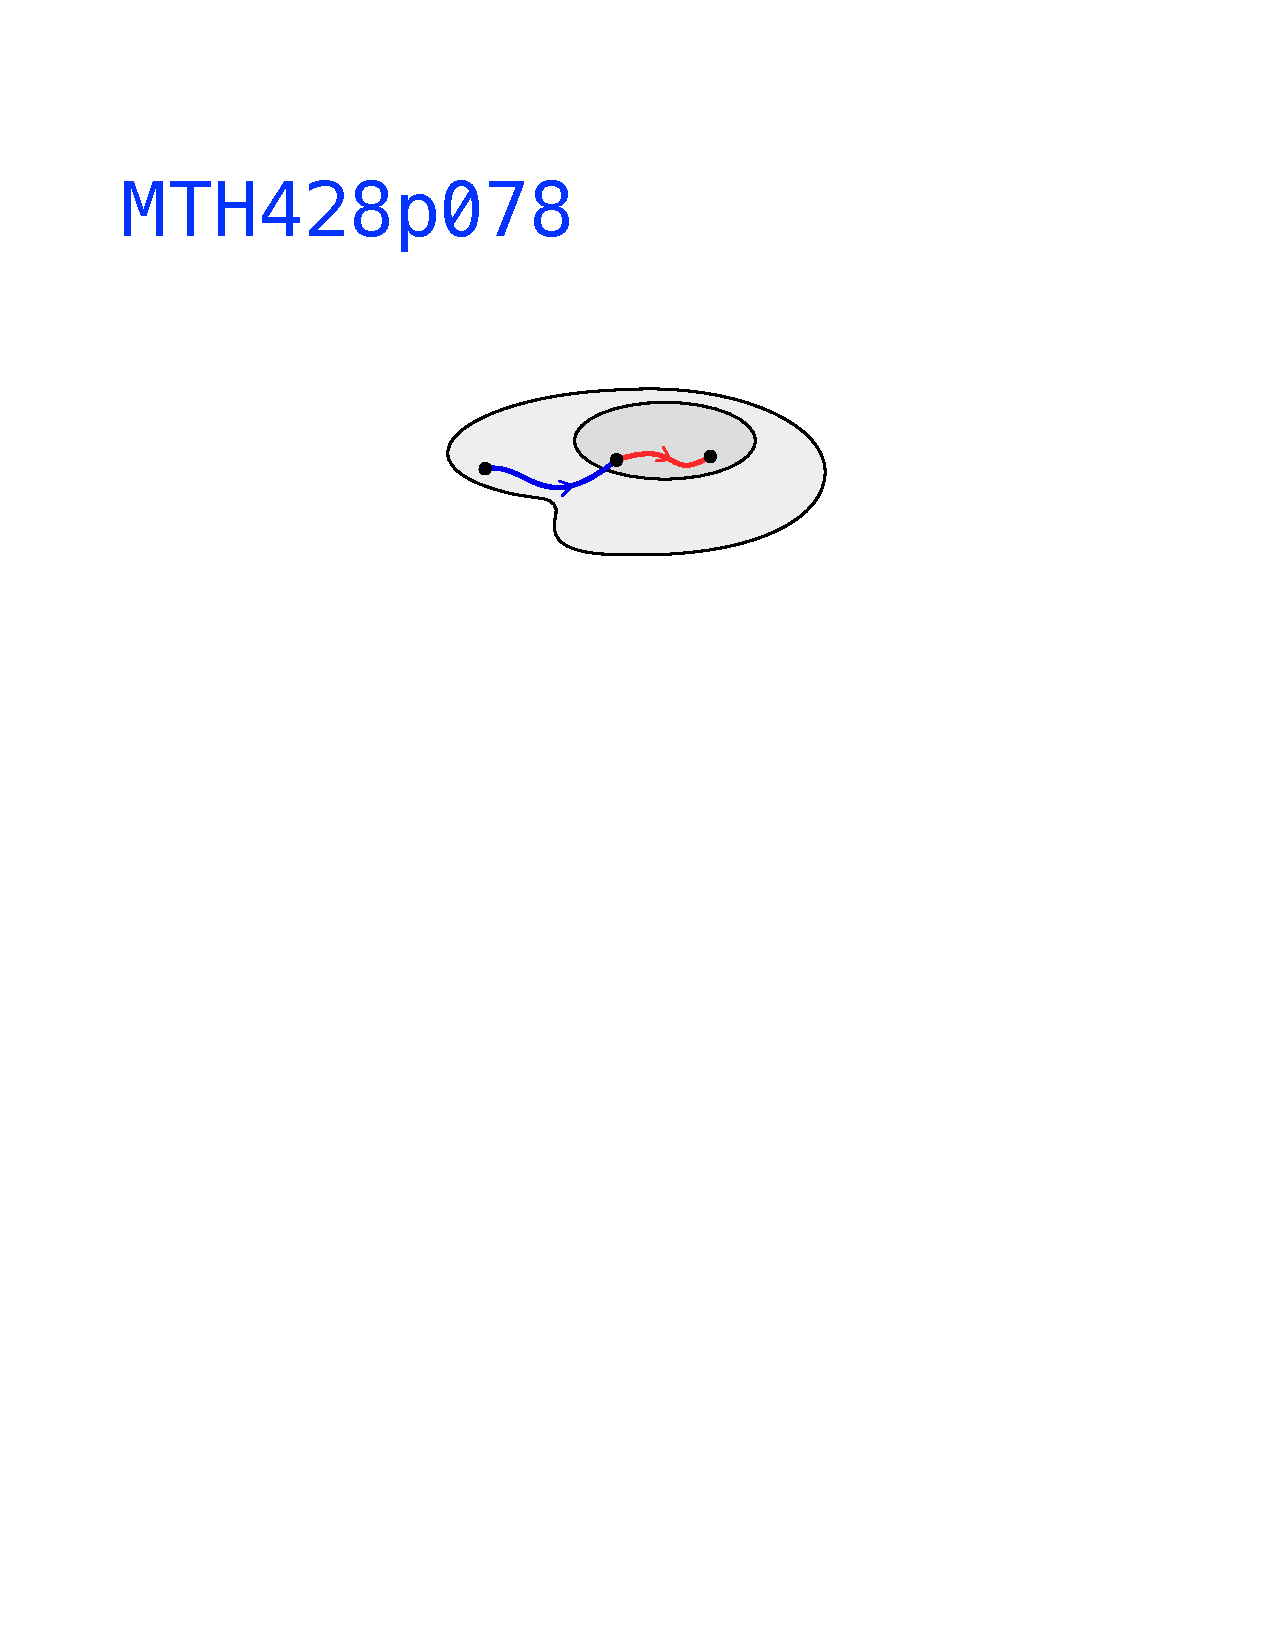
\includegraphics[width=\textwidth, trim=0mm 185mm 0mm 63mm, clip]{pictures/MTH428p078.pdf}}};

%%% COORDINATE GRID
%\draw[step=0.5, help lines] (0,0) to[grid with coordinates] (15,9);
%%% 
\node[anchor= base]  at (6.33 , 1.3){\small  $x_{0}$};
\node[anchor= base]  at (7.3 , 1.1){\small  \color{blue} $\omega$};
\node[anchor= base]  at (8.6 , 1.5){\small  \color{red} $\alpha$};
\node[anchor= base]  at (7.8 , 1.5){\small  $U$};

\end{tikzpicture}
\end{equation*}
One can check that  the collection of all sets $U[\omega]$ defined in this way is a basis of a topology 
on $\nwidetilde X$ (exercise). We will consider $\nwidetilde X$ as a topological space with topology defined by this basis. 

Consider the function $p\colon \nwidetilde X \to X$ given by $p([\omega]) = \omega(1)$. We will show that 
this is a universal covering of $X$. We will use the following observations, proofs of which are left as an exercise: 

{\bf (i)} For any trivial set $U\subseteq X$ and any path $[\omega]\in \nwidetilde X$ such that $\omega(1) \in U$
the map 
$$p|_{U[\omega]}\colon U[\omega] \to U$$ 
is a homeomorphism. 

{\bf (ii)} Let $U\subseteq X$ be a trivial set, let $x\in U$ and let 
$H(x_{0}, x) = \{ [\omega]\in\nwidetilde X \ | \  \omega(1) = x\}$.
Then
$$p^{-1}(U) = \bigcup_{[\omega] \in H(x_{0}, x)} U[\omega]$$
Moreover $U[\omega] \cap U[\omega'] = \varnothing$ for all $[\omega], [\omega']\in H(x_{0}, x)$, 
$[\omega]\neq [\omega']$. 

{\bf (iii)}  For a path  $\omega\colon [0, 1] \to X$ such that $\omega(0) = x_{0}$  and  for $s\in [0, 1]$ let 
$\omega_{s}$ be the path in $X$ defined by $\omega_{s}(t) = \omega(st)$.  The function 
$h_{\omega}\colon [0, 1] \to \nwidetilde X$ given by  $h_{\omega}(s) = [\omega_{s}]$ is continuous. 


Directly from (ii) is follows that the function $p$ is continuous. Furthermore, combining (ii) and (i) we obtain 
that $p$ is covering and that each trivial set in $X$ is evenly covered by $p$. 

Next, by (iii) the space 
$\nwidetilde X$ is path connected. Indeed, for any $[\omega]\in \nwidetilde X$  the function $h_{\omega}$
is a path in $\nwidetilde X$ joining $[\omega]$ with $[c_{x_{0}}]$, the homotopy class of the constant path at $x_{0}$. 
It remains then to show that the fundamental group $\pi_{1}(\nwidetilde X, [c_{x_{0}}])$ is trivial, or equivalently 
that $p_{\ast}(\pi_{1}(\nwidetilde X, [c_{x_{0}}]))$ is the trivial subgroup of $\pi_{1}(X, x_{0})$.  Assume then that
$\omega$ is a loop in $X$ such that $[\omega]\in p_{\ast}(\pi_{1}(\nwidetilde X, [c_{x_{0}}]))$. By 
Theorem \ref{COVERINGSUBGP THM}  this means that the lift of $\omega$ to $\nwidetilde X$ that starts at 
$[c_{x_{0}}]$ is a loop in $\nwidetilde X$. Notice, however, that this lift is given the path $h_{s}$ defined in (iii). 
This path is a loop only when $[c_{x_{0}}] = h_{\omega}(0) = h_{\omega}(1) = [\omega]$ i.e. only when 
$[\omega]$ is the trivial element of $\pi_{1}(X, x_{0})$. 


\end{proof}



%%%%%%%%%%%%%%%%%%%%%%%%%%%%%%%
%  EXERCISES
%%%%%%%%%%%%%%%%%%%%%%%%%%%%%%%

\exercises

\begin{exercise}
Prove Proposition \ref{UNIVCOVERING NECESSARY COND PROP}. 
\end{exercise}

\begin{exercise}
Let $X$, $Y$ be connected and locally path connected spaces, and let 
$\tilde{p}_{X}\colon \widetilde{X} \to X$, and  $\tilde{p}_{Y}\colon \widetilde{Y} \to Y$ be their 
universal coverings. Show that if $X\simeq Y$ then $\widetilde{X} \simeq \widetilde{Y}$. 
\end{exercise}


\begin{exercise}
Describe explicitly all non-isomorphic coverings of the space $\R P^{2}\times \R P^{2}$
\end{exercise}




\begin{exercise}
Let $X$ be a space, and let $A\subseteq X$. Assume that both $X$ and $A$ are connected
and locally path connected, and that the inclusion map $i\colon A \to X$ induces an isomorphism 
of the fundamental groups 
$$i_{\ast} \colon \pi_{1}(A, x_{0}) \overset{\cong}{\lra} \pi_{1}(X, x_{0})$$
for $x_{0}\in A$. Show that if $\tilde{p}\colon \widetilde{X} \to X$ is a universal covering of $X$ then 
the map $\tilde{p}|_{\tilde{p}^{-1}(A)}\colon \tilde{p}^{-1}(A) \to A$ is a universal covering of $A$. 
\end{exercise}

\begin{exercise}
a) Let $X$ be a finite, path connected,  1-dimensional CW-complex. Show that if  $\tilde{p} \colon \widetilde{X} \to X$ is 
the universal covering of $X$ then the space $\widetilde{X}$ has the structure of a 1-dimensional CW-complex such that 
$\tilde{p}$ is a cellular map. 

b)  Use part a) to show that if $F$ is a finitely generated free group then every subgroup of $F$ is free. 

c) Recall that  $[G:H]$ denotes the index of a subgroup $H$ in a group $G$. 
Let $F$ be free group on $n$ generators, and let $H$ be a subgroup of  $F$. Show that if $[F:H] = k$ then $H$ is a free 
group on $(n-1)k + 1$ generators. 
\end{exercise}






\newpage
%%%%%%%%%%%%%%%%%%%%%%%%%%%%%%%
%%%%%%%%%%%%%%%%%%%%%%%%%%%%%%%
%%%
%%%  EQUIVALENCES OF CATEGORIES
%%%
%%%%%%%%%%%%%%%%%%%%%%%%%%%%%%%
%%%%%%%%%%%%%%%%%%%%%%%%%%%%%%%

 %---BBLANK
\chapter[Equivalences of Categories]{Equivalences \\ of Categories}
 %---EBLANK
\chaptermark{Equivalences of Categories}
\label{CAT EQUIV  CHAPTER}


\thispagestyle{firststyle}


Results of Chapters \ref{CLASS OF COV CHAPTER} and \ref{FROM SUBGP TO COV CHAPTER}
can be summarized as follows:

 %---BBLANK
\begin{theorem}
\label{COMPLETE CLASSIF OF COVERINGS THM}
Let $X$ be a connected, locally path connected, and semi-locally simply connected space, and 
let $x_{0}\in X$. The map
\begin{center}
\begin{tabular}{ccc}
$
\Omega\colon
\begin{pmatrix}
\text{\ \ isomorphism classes\ \ } \\[1mm]
\text{of path connected} \\[1mm]
\text{coverings of $X$} \\
\end{pmatrix}
$
& 
$\lra$
&
$ 
\begin{pmatrix}
\text{\ \ conjugacy classes\ \ } \\[1mm]
\text{of subgroups} \\[1mm]
\text{of $\pi_{1}(X, x_{0})$} \\
\end{pmatrix}
$
\end{tabular}
\end{center}
given by $\Omega(p\colon T\to X) = p_{\ast}(\pi_{1}(T, \tilde{x}))$ for some $\tilde{x}\in p^{-1}(x_{0})$
is a bijection.
\end{theorem}
 %---EBLANK # \newpage


\begin{proof}
The map $\Omega$ is 1-1 by Theorem \ref{CLASSOFCOVERINGS THM}, and it is onto 
by  Theorems \ref{UNIVCOVERGIVESALL THM} and \ref{UNIV COV EXISTENCE THM}. 
\end{proof}

Theorem \ref{COMPLETE CLASSIF OF COVERINGS THM} translates the topological problem 
of classifying coverings into an algebraic one, of identifying conjugacy classes of subgroups 
of a group. However,  since coverings over $X$ form a category $\Cov(X)$, with morphisms given by maps 
of coverings, a more complete correspondence between  topology and algebra would be obtained if we 
could find some algebraic category $\DD$ and a functor  
$$F \colon \Cov(X) \to \DD$$ 
that would let us restate problems about coverings and maps of coverings as problems about objects and morphism 
of the category $\DD$. In Chapter \ref{COV AND GROUP ACT  CHAPTER} we will show that such 
category $\DD$ and a functor $F$ exist. Before we get to this though, we need to consider what properties 
the functor $F$ should have so that it would allow us to go back and forth between categories $\Cov(X)$ and 
$\DD$ without losing any essential information. The most obvious requirement is that $F$ should be an 
isomorphism of categories, i.e. that there should exist a functor $G\colon \DD \to \Cov(X)$ such the compositions
$GF\colon \Cov(X) \to \Cov(X)$ and $FG\colon \DD\to \DD$ are identies on all objects and morphisms. 
It turns out however, that isomorphisms of categories appear very rarely in practical applications. 
A somewhat weaker but much more useful notion is an equivalence of categories:

 %---BBLANK
\begin{definition}
\label{CAT EQUIVALNCE DEF}
A functor $F\colon \CC \to \DD$ is an \emph{equivalence of categories} if there exists a functor 
$G\colon \DD\to \CC$ for which the following conditions hold:
\begin{itemize}
\item[1)] For each object $c\in \CC$ there exists an isomorphism $\eta_{c}\colon c \to GF(c)$ 
such that for any morphism $f\colon c \to c'$ the following diagram commutes:
\begin{equation*}
\begin{tikzpicture}
\matrix (m) 
[matrix of math nodes, row sep=3em, column sep=3em, text height=1.5ex, text depth=0.25ex]
{
c & c' \\
GF(c) & GF(c') \\
};
\path[->, thick, font=\scriptsize]
(m-1-1) 
edge node[auto] {$f$} (m-1-2)
edge node[anchor = east] {$\eta_{c}$} node[anchor = west] {$\cong$} (m-2-1)
(m-1-2)
edge node[anchor=  west] {$\eta_{c'}$} node[anchor = east] {$\cong$} (m-2-2)
(m-2-1)
edge node[anchor=  north] {$GF(f)$} (m-2-2)
; 
\end{tikzpicture}
\end{equation*}

\item[2)] For each object $d\in \DD$ there exists an isomorphism $\tau_{d}\colon d \to FG(d)$ 
such that for any morphism $g\colon d \to d'$ the following diagram commutes:
\begin{equation*}
\begin{tikzpicture}
\matrix (m) 
[matrix of math nodes, row sep=3em, column sep=3em, text height=1.5ex, text depth=0.25ex]
{
d & d' \\
FG(d) & FG(d') \\
};
\path[->, thick, font=\scriptsize]
(m-1-1) 
edge node[auto] {$g$} (m-1-2)
edge node[anchor = east] {$\tau_{d}$} node[anchor = west] {$\cong$} (m-2-1)
(m-1-2)
edge node[anchor=  west] {$\tau_{d'}$} node[anchor = east] {$\cong$} (m-2-2)
(m-2-1)
edge node[anchor=  north] {$FG(g)$} (m-2-2)
; 
\end{tikzpicture}
\end{equation*}
\end{itemize}
We will say that $\CC$ and $\DD$ are \emph{equivalent categories} if there exists an equivalence $\CC\to \DD$. 
\end{definition}
 %---EBLANK # \newpage


The following fact is often useful, since it allows us to check if a functor is an equivalence of categories without 
constructing the inverse functor $G$.

 %---BBLANK
\begin{proposition}
\label{CAT EQUIV PROP}
A functor $F\colon \CC \to \DD$ is an equivalence of categories if and only if the following conditions hold. 
\benu
\item[(i)] For each object $d\in \DD$ there exists an object $c\in \CC$ such that $d\cong F(c)$. 
\item[(ii)] For any objects $c, c'\in \CC$ the map $\Mor_{\CC}(c, c') \to \Mor_{\DD}(F(c), F(c'))$ given by 
$f\mapsto F(f)$ is a bijection.
\eenu

\end{proposition}

\begin{proof}
Exercise. 
\end{proof}
 %---EBLANK # \newpage

\begin{example}
Let $\mathbf{FVect(\R)}$ denote the category of finitely dimensional real vector spaces with linear transformations 
as morphisms. Also, let $\mathbf{M(\R)}$ denote the category whose objects are natural numbers $0, 1, 2, \dots$. 
The set of morphisms $\Mor_{\mathbf{M(\R)}}(n, m)$ consists of all $n\times m$ matrices with real coefficients. 
Composition of morphisms is given by matrix multiplication. 
We have a functor
$$F\colon \mathbf{M(\R)} \to \mathbf{FVect(\R)}$$
defined as follows. On objects  $F(n) = \R^{n}$. If $A$ is an $n\times m$ matrix  (i.e. a morphism $n\to m$ in 
$\mathbf{M(\R)}$) then $F(A)\colon \R^{n}\to \R^{m}$
is a linear transformation given by $F(A)(v) = Av$ for $v\in \R^{n}$.  One can show that $F$ is an equivalence of 
categories (exercise). 
\end{example}

\begin{example}
Recall (\ref{FUND GROUPOID DEF}) that the fundamental groupoid of a space $X$ is a category $\Pi_{1}(X)$
whose objects are points of $X$. For $x, x'\in X$ morphisms $x\to x'$ are homotopy classes of paths that begin
at $x$ and end at $x'$. Composition of morphisms is given by concatenation of paths. A map of spaces 
$f\colon X \to X'$ induces a functor of fundamental groupoids $f_{\ast}\colon \Pi_{1}(X) \to \Pi_{1}(X')$. 
One can show that if $f$ is a homotopy equivalence of spaces then the functor $f_{\ast}$ is an equivalence 
of categories (exercise). 
\end{example}

%%%%%%%%%%%%%%%%%%%%%%%%%%%%%%%
%  EXERCISES
%%%%%%%%%%%%%%%%%%%%%%%%%%%%%%%

\exercises

\begin{exercise}
Prove Proposition \ref{CAT EQUIV PROP}.
\end{exercise}





\newpage
%%%%%%%%%%%%%%%%%%%%%%%%%%%%%%%
%%%%%%%%%%%%%%%%%%%%%%%%%%%%%%%
%%%
%%%  COVERINGS AND GROUP ACTIONS
%%%
%%%%%%%%%%%%%%%%%%%%%%%%%%%%%%%
%%%%%%%%%%%%%%%%%%%%%%%%%%%%%%%

 %---BBLANK 
\chapter[Coverings and Group Actions]{Coverings\\ and  Group Actions}
 %---EBLANK
\chaptermark{Coverings and Group Actions}
\label{COV AND GROUP ACT  CHAPTER}

Let $X$ be a topological space, and let $x_{0}\in X$. Our goal in this chapter is to show that under 
some assumptions on $X$ the category of path connected coverings of $X$ is equivalent to the category 
of sets equipped with a transitive action of the group $\pi_{1}(X, x_{0})$. 

 %---BBLANK
\begin{definition}
\label{RIGHT GP ACTION DEF}
Let $G$ be a group and $S$ be a set. We say that $G$ \emph{acts on} $X$ on the right if there exists 
a function 
$$\mu\colon S \times G \to S$$
such that 
\benu
\item[(i)] $\mu(s, e) = s$ for any $s\in S$, where $e\in G$ is the trivial element;  
\item[(ii)] $\mu(\mu(s, g), h) = \mu(s, gh)$ for all $s\in S$, $h, g\in G$. 
\eenu
\end{definition}
 %---EBLANK # \newpage

\begin{note}
From now on we will write $sg$ instead of $\mu(s, g)$ in order to describe the action of $g$ on $s$. 
We will also  refer to sets with an action of a group $G$ as $G$-sets. 
\end{note}

\begin{example}
Let $p\colon T\to X$ be a covering and let $x_{0}\in X$. We can define a right action of $\pi_{1}(X, x_{0})$
on the fiber $p^{-1}(x_{0})$ as follows. For $[\omega]\in \pi_{1}(X, x_{0})$ and $y\in p^{-1}(x_{0})$ let 
$\nwidetilde \omega\colon [0, 1] \to T$ be the lift of $\omega$ such that $\nwidetilde \omega(0) = y$. 
Define:
$$y[\omega] := \nwidetilde \omega(1)$$
One can check that this  satisfies the conditions of Definition \ref{RIGHT GP ACTION DEF} (exercise). 
The action of $\pi_{1}(X, x_{0})$ on $p^{-1}(x_{0})$ defined in this way is called the \emph{monodromy action} 
associated to the covering $p$. 
\end{example}

  %---BBLANK 
\begin{definition}
We say that a group $G$ acts on set $S$ \emph{transitively} if for any $s, s'\in S$ there exists 
$g\in G$ such that $sg = s'$. 
\end{definition}
 %---EBLANK  # \vskip 30mm

 %---BBLANK
\begin{proposition}
\label{TRANSITIVE MONODROMY PROP}
Let $p\colon T \to X$ be a covering, and let $x_{0}\in X$. If $T$ is path connected then the monodromy 
action of  $\pi_{1}(X, x_{0})$ on $p^{-1}(x_{0})$ is transitive.
\end{proposition}

\begin{proof}
Exercise. 
\end{proof}
 %---EBLANK  # \newpage

 %---BBLANK
\begin{definition}
Let $G$ be a group and let $S, S'$ be $G$-sets. A function 
$f\colon S \to S'$ is \emph{$G$-equivariant} if $f(sg) = f(s)g$ for all $s\in S$ and $g\in G$.   
\end{definition}
 %---EBLANK  # \vskip 80mm

 %---BBLANK
\begin{note}
$G$-sets and $G$-equivariant functions form a category which we will denote
by $\Set_{G}$. 
\end{note}
 %---EBLANK  # \vskip 30mm

 %---BBLANK
\begin{proposition}
\label{MAP OF COVERINGS EQUIV PROP}
Let $X$ be a space, and let 
\begin{equation*}
\begin{tikzpicture}
\matrix (m) 
[matrix of math nodes, row sep= 2.5em, column sep=1.5em, text height=1.5ex, text depth=0.25ex]
{
T_{1} &  &  T_{2} \\
 & X & \\
};
\path[->, thick, font=\scriptsize]
(m-1-1) 
edge node[auto] {$f$} (m-1-3)
edge node[anchor = north east] {$p_{1}$} (m-2-2)
(m-1-3) 
edge node[anchor = north west] {$p_{2}$} (m-2-2)
;
\end{tikzpicture}
\end{equation*}
be a map of coverings. For any $x_{0}\in X$ the induced map of fibers 
$f\colon p_{1}^{-1}(x_{0}) \to p_{2}^{-1}(x_{0})$ is $\pi_{1}(X, x_{0})$-equivariant. 
\end{proposition}

\begin{proof}
Exercise.
\end{proof}
 %---EBLANK  # \newpage


 %---BBLANK
\begin{corollary}
Let $X$ be a space and let $x_{0}\in X$. The assignment which associates to each path connected 
covering $p\colon T\to X$ the $\pi_{1}(X, x_{0})$-set $p^{-1}(x_{0})$ and to each map of coverings the 
map of fibers defines a functor
$$\Lambda\colon \Cov(X)  \to \Set_{\pi_{1}(X, x_{0})}$$
\end{corollary}

\begin{proof}
Exercise.
\end{proof}
 %---EBLANK

For the reminder of this chapter we will be restrict attention to coverings $T\to X$ where $T$ is 
a path connected space. Let $ \PCov(X) $ denote the category of all such covering of $X$. 
Also, for a group $G$ let $\TSet_{G}$ denote the category of all $G$-sets with a transitive action of 
$G$. By Proposition \ref{TRANSITIVE MONODROMY PROP} the functor $\Lambda$ restricts to 
a functor
$$\Lambda\colon \PCov(X)  \to \TSet_{\pi_{1}(X, x_{0})}$$

Our next goal is to show that the following holds:

 %---BBLANK # \vskip 90mm
\begin{theorem}
\label{PCOV EQ TSET THM}
Let $X$ be a connected, locally path connected, and semi-locally simply connected space, and let 
$x_{0}\in X$.  The functor
$$\Lambda\colon \PCov(X)  \to \TSet_{\pi_{1}(X, x_{0})}$$
is an equivalence of categories. 
\end{theorem}
 %---EBLANK  # \newpage


By Proposition \ref{CAT EQUIV PROP} the proof of Theorem \ref{PCOV EQ TSET THM} can be split into two 
parts:

 %---BBLANK # Outline of proof of Theorem \ref{PCOV EQ TSET THM}:
1) We need to show that  any set with a transitive action of the group $\pi_{1}(X, x_{0})$ is isomorphic
to a $\pi_{1}(X, x_{0})$-set $\Lambda(p\colon T \to X)=p^{-1}(x_{0})$ for some path connected covering $p$. 

2) We also need to show that maps of path connected coverings of $X$ are in a bijective correspondence with 
$\pi_{1}(X, x_{0})$-equivariant maps of their fibers.  
 %---EBLANK 

Part 1) will follow immediately from the following  result:



 %---BBLANK  # \vskip 80mm
\begin{proposition}
\label{ISO COVERINGS ISO G-SETS PROP}
Let $X$ be a connected, locally path connected, and semi-locally simply connected space and let 
$x_{0}\in X$. The map
 \begin{center}
\begin{tabular}{ccc}
$
\Lambda\colon 
\begin{pmatrix}
\text{\ \ isomorphism classes\ \ } \\[1mm]
\text{of path connected} \\[1mm]
\text{coverings of $X$} \\
\end{pmatrix}
$
& 
$\lra$
&
$ 
\begin{pmatrix}
\text{\ \ isomorphism classes\ \ } \\[1mm]
\text{of sets with transitive} \\[1mm]
\text{action of $\pi_{1}(X, x_{0})$} \\
\end{pmatrix}
$
\end{tabular}
\end{center}
given by $\Lambda(p\colon T\to X) = p^{-1}(x_{0})$ is a bijection. 
\end{proposition}
 %---EBLANK # \newpage


The proof of Proposition \ref{ISO COVERINGS ISO G-SETS PROP} will use  
some properties of transitive $G$-sets that we develop below. 


 %---BBLANK 
\begin{definition}
Let $G$ be a group,  and $S$ be a $G$-set. The \emph{stabilizer} of en element $s\in S$ is the subgroup 
$G_{s}\subseteq G$ given by:
$$G_{s} = \{ g\in G \ | \ sg = s\}$$ 
\end{definition}
 %---EBLANK  # \vskip 30mm

 %---BBLANK 
\begin{proposition}
\label{STAB OF MONODROMY PROP}
Let $p\colon T\to X$ be a covering, and let $x_{0}\in X$. The stabilizer of an element $\ntilde x \in p^{-1}(x_{0})$
under the monodromy action is the subgroup $p_{\ast}(\pi_{1}(T, \ntilde x)) \subseteq \pi_{1}(X, x_{0})$.
\end{proposition}

\begin{proof}
Exercise. 
\end{proof}
 %---EBLANK # \vskip 50mm

 %---BBLANK 
\begin{lemma}
\label{TRANS GROUP ACTION CLASSIF LEMMA}
Let $G$ be a group. 
\benu
\item[1)] If $G$ acts transitively on a set $S$ and $s, s'\in S$ then the stabilizers $G_{s}$ and $G_{s'}$
are conjugate subgroups of the group $G$. 
\item[2)]  Let $S$ be a set with an action of $G$ and let $s\in S$. The assignment $S \mapsto G_{s}$ 
defines a bijective correspondence: 
\begin{center}
\begin{tabular}{ccc}
$
\Phi\colon 
\begin{pmatrix}
\text{\ \ isomorphism classes\ \ } \\[1mm]
\text{of sets with a transitive} \\[1mm]
\text{action of $G$} \\
\end{pmatrix}
$
& 
$\lra$
&
$ 
\begin{pmatrix}
\text{\ \ conjugacy classes\ \ } \\[1mm]
\text{of subgroups} \\[1mm]
\text{of $G$} \\
\end{pmatrix}
$
\end{tabular}
\end{center}
\eenu
\end{lemma}
 %---EBLANK # \newpage


\begin{proof}
1) Since $G$ acts transitively we have $s' = sh$ for some $h\in G$. We will show that 
$G_{s'} = h^{-1}G_{s}h$. For $g\in G_{s}$  we have: 
$$s'(h^{-1}gh) = sgh = sh = s'$$
Therefore $h^{-1}G_{s}h\subseteq G_{s'}$. Conversely, if $g\in G_{s'}$ then 
$$sh = s' =  s'g = shg$$
This implies that $s = s(hgh)^{-1}$, so $hgh^{-1}\in G_{s}$, or equivalently 
$g\in h^{-1}G_{s}h$. Thus $G_{s'} \subseteq h^{-1}G_{s}h$.


2) We will construct a function 
\begin{center}
\begin{tabular}{ccc}
$ 
\Psi\colon
\begin{pmatrix}
\text{\ \ conjugacy classes\ \ } \\[1mm]
\text{of subgroups} \\[1mm]
\text{of $G$} \\
\end{pmatrix}
$
& 
$\lra$
&
$
\begin{pmatrix}
\text{\ \ isomorphism classes\ \ } \\[1mm]
\text{of sets with transitive} \\[1mm]
\text{action of $G$} \\
\end{pmatrix}
$
\end{tabular}
\end{center}
which is the inverse of $\Phi$.
For a  subgroup $H\subseteq G$ let $H\backslash G$  denote the set of right cosets of 
$H$ in $G$. Define an action of $G$ on $H\backslash G$ by $(Hg)g' = H(gg')$. This action is transitive 
since for any $Hg, Hg'\in H\backslash G$ we have $Hg' = (Hg)(g^{-1}g')$. Let $\Psi(H) = H\backslash G$.
In order to show that $\Psi$ is well defined on conjugacy classes we need to check that if 
$H' \subseteq G$ is a subgroup conjugate to $H$ then the $G$-sets $H\backslash G$ and $H'\backslash G$ are isomorphic. 
Assume then that  $H' = kHk^{-1}$ for some $k\in G$. Define 
$f\colon  H\backslash G \to H'\backslash G$ by $f(Hg) = H'kg$. One can check that this is a well 
defined isomorphism of $G$-sets (exercise).  Let $e\in G$  be the trivial element. Since the stabilizer 
of $He\in H\backslash G$ is the subgroup $H$, we obtain that $\Phi\Psi([H]) = [H]$ where $[H]$ denotes 
the conjugacy class of $H$, and so $\Phi\Psi$ is an identity function. One can check that the composition 
$\Psi\Phi$ also is an identity (exercise).  

\end{proof}



\begin{proof}[Proof of Proposition \ref{ISO COVERINGS ISO G-SETS PROP}]
Consider the diagram:
\begin{equation*}
\begin{tikzpicture}
\matrix (m) 
[matrix of math nodes, row sep= 3em, column sep= -2em, text height=5ex, text depth=4.25ex]
{
 \begin{pmatrix}
\text{\ \ isomorphism classes\ \ } \\[1mm]
\text{of path connected} \\[1mm]
\text{coverings of $X$} \\
\end{pmatrix}
& & 
 \begin{pmatrix}
\text{\ \ isomorphism classes\ \ } \\[1mm]
\text{of sets with transitive} \\[1mm]
\text{action of $\pi_{1}(X, x_{0})$} \\
\end{pmatrix} 
\\
& 
\begin{pmatrix}
\text{\ \ conjugacy classes\ \ } \\[1mm]
\text{of subgroups} \\[1mm]
\text{of $\pi_{1}(X, x_{0})$} \\
\end{pmatrix}
& 
\\ 
};
\path[->, thick]
(m-1-1) 
edge node[anchor = south] {$\Lambda$} (m-1-3)
edge node[anchor= north east] {$\Omega$} (m-2-2)
;
\path[->, thick]
(m-1-3) 
edge node[anchor=north west] {$\Phi$} (m-2-2)
; 
\end{tikzpicture}
\end{equation*}
The map $\Phi$ is defined as in proposition \ref{TRANS GROUP ACTION CLASSIF LEMMA}, and 
and $\Omega$ is defined as in Theorem \ref{COMPLETE CLASSIF OF COVERINGS THM}. By 
Proposition \ref{STAB OF MONODROMY PROP} this diagram commutes. Since $\Phi$ is a bijection 
by Proposition \ref{TRANS GROUP ACTION CLASSIF LEMMA}, and $\Omega$ is a bijection by 
Theorem \ref{COMPLETE CLASSIF OF COVERINGS THM} we obtain that $\Lambda$ is a bijection. 
\end{proof}


Next, we turn to  properties of the functor $\Lambda$ related to maps of coverings. We will show that 
the following holds. 

 %---BBLANK 
\begin{proposition}
\label{BIJ MAPS OF COV TO EQUIV MAPS PROP}
Let $X$ be a connected and locally path connected space, and let $x_{0}\in X$. For any path connected coverings 
$p_{i}\colon T_{i}\to X$, $i=1,2$
the assignment 
\begin{center}
\begin{tabular}{ccc}
$
\Lambda\colon
\begin{pmatrix}
\text{\ \ maps of coverings\ \ } \\[1mm]
T_{1}\to T_{2} \\
\end{pmatrix}
$
& 
$\lra$
&
$ 
\begin{pmatrix}
\text{\ \ $\pi_{1}(X, x_{0})$-equivariant maps\ \ } \\[1mm]
p_{1}^{-1}(x_{0}) \to p_{2}^{-1}(x_{0}) \\
\end{pmatrix}
$
\end{tabular}
\end{center}
is a bijection.
\end{proposition}
  %---EBLANK # \vskip 30mm

The proof of Proposition \ref{BIJ MAPS OF COV TO EQUIV MAPS PROP} will use the following fact. Recall that 
for a $G$-set $S$ by $G_{s}$ we denote the stabilizer of an element $s\in S$

 %---BBLANK 
\begin{lemma}
\label{EQUIV MAP CLASSIFIC LEMMA}
Let $S$, $T$ be sets with a transitive action of a group $G$, and let $s_{0}\in S$, $t_{0}\in T$. 
A $G$-equivariant map $f\colon S\to T$ such that $f(s_{0}) = t_{0}$ exists if and only if $G_{s_{0}} \subseteq G_{t_{0}}$. 
Moreover, if such map exists then it is unique.
\end{lemma}
 %---EBLANK  # \newpage

\begin{proof}
Exercise. 
\end{proof}

\begin{proof}[Proof of Proposition \ref{BIJ MAPS OF COV TO EQUIV MAPS PROP}]
We will prove first that $\Lambda$ is onto. 
Let $f\colon p_{1}^{-1}(x_{0}) \to p_{2}^{-1}(x_{0})$ be a $\pi_{1}(X, x_{0})$-equivariant map. We need to 
show that there exists a map of coverings $\bar{f}\colon T_{1}\to T_{2}$ such that $\Lambda(\xov{f}) = f$. 
Let $\tilde{x}_{1} \in p_{1}^{-1}(x_{0})$, and  let $\tilde{x}_{2} = f(\tilde{x}_{1})$. Combining 
Proposition \ref{STAB OF MONODROMY PROP} and Lemma \ref{EQUIV MAP CLASSIFIC LEMMA} we obtrain
$$p_{1\ast}(\pi_{1}(T_{1}, \tilde{x}_{1}))\subseteq p_{2\ast}(\pi_{1}(T_{2}, \tilde{x}_{2}))$$
Therefore, by the lifting criterion (\ref{LIFTINGCRIT THM}) there exists a map of coverings 
$\bar{f}\colon T_{1}\to T_{2}$ such that $f(\tilde{x}_{1}) = \tilde{x_{2}}$. Since the map 
$\Lambda(\bar{f})\colon p_{1}^{-1}(x_{0}) \to p_{2}^{-1}(x_{0})$ satisfies $\Lambda(\bar{f})(\tilde{x}_{1}) = \tilde{x}_{2}$ 
the uniqueness part of Lemma \ref{EQUIV MAP CLASSIFIC LEMMA} gives $\Lambda(\bar{f}) = f$. 

Next, assume that $f, f'\colon T_{1}\to T_{2}$ are maps of coverings such that $\Lambda(f) = \Lambda(f')$. 
This implies that for $\tilde{x} \in p^{-1}(x_{0})$ we have 
$$f(\tilde{x}) = \Lambda(f)(\tilde{x}) =  \Lambda(f')(\tilde{x}) = f'(\tilde{x})$$
By Lemma \ref{COVERINGUNIQUELIFT LEMMA} this gives $f=f'$. 

\end{proof}


\begin{proof}[Proof of Theorem \ref{PCOV EQ TSET THM}]
Follows directly from Propositions \ref{CAT EQUIV PROP},   \ref{ISO COVERINGS ISO G-SETS PROP}
and  \ref{BIJ MAPS OF COV TO EQUIV MAPS PROP}.
\end{proof}


%%%%%%%%%%%%%%%%%%%%%%%%%%%%%%%
%  EXERCISES
%%%%%%%%%%%%%%%%%%%%%%%%%%%%%%%

\vskip -10mm

\exercises


\begin{exercise}
Prove Proposition \ref{TRANSITIVE MONODROMY PROP}. 
\end{exercise}


\begin{exercise}
Prove Proposition \ref{MAP OF COVERINGS EQUIV PROP}. 
\end{exercise}

\begin{exercise}
Prove Proposition \ref{STAB OF MONODROMY PROP}. 
\end{exercise}


\begin{exercise}
Prove Lemma \ref{EQUIV MAP CLASSIFIC LEMMA}. 
\end{exercise}


\newpage
%%%%%%%%%%%%%%%%%%%%%%%%%%%%%%%
%%%%%%%%%%%%%%%%%%%%%%%%%%%%%%%
%%%
%%%  DECK TRANSFORMATIONS
%%%
%%%%%%%%%%%%%%%%%%%%%%%%%%%%%%%
%%%%%%%%%%%%%%%%%%%%%%%%%%%%%%%

 %---BBLANK 
\chapter[Deck Transformations]{Deck \\ Transformations}
 %---EBLANK 
\chaptermark{Deck Transformations}
\label{DECK TRANSF  CHAPTER}


 %---BBLANK 
\begin{definition}
Let $p\colon T \to X$ be a covering. A \emph{deck transformation} of $p$ is an isomorphism of coverings 
\begin{equation*}
\begin{tikzpicture}
\matrix (m) 
[matrix of math nodes, row sep= 2.5em, column sep=1.5em, text height=1.5ex, text depth=0.25ex]
{
T &  &  T \\
 & X & \\
};
\path[->, thick, font=\scriptsize]
(m-1-1) 
edge node[anchor=south] {$f$} node[anchor=north] {$\cong$}(m-1-3)
edge node[anchor = north east] {$p$} (m-2-2)
(m-1-3) 
edge node[anchor = north west] {$p$} (m-2-2)
;
\end{tikzpicture}
\end{equation*}
\end{definition}
 %---EBLANK  # \newpage

Deck transformations form a group under composition of isomorphisms. We will denote this group by $D(p)$.
In this chapter we will compute the group $D(p)$ for a path connected covering $p$ in terms of fundamental
groups of $X$ and $T$. Recall that in Chapter \ref{COV AND GROUP ACT  CHAPTER}  we constructed 
a functor $$\Lambda\colon \PCov(X)  \to \TSet_{\pi_{1}(X, x_{0})}$$ from the category of path connected 
coverings of a space $X$ to the category of transitive $\pi_{1}(X, x_{0})$-sets. We also showed 
(\ref{BIJ MAPS OF COV TO EQUIV MAPS PROP}) that if $X$ is a connected and locally path connected space 
then this functor is a bijection of sets of morphisms.  Since any functor preserves isomorphism, if 
$f:T_{1}\to T_{2}$ is an isomorphism of coverings of $X$, then $\Lambda(f)$ is an isomorphism of 
$\pi_{1}(X, x_{0})$-sets. The following fact implies that the converse is also true:

 %---BBLANK 
\begin{lemma}
Let $F\colon \CC \to \DD$ be a functor such that for any $c, c'\in \CC$ the map 
the map $\Mor_{\CC}(c, c') \to \Mor_{\DD}(F(c), F(c'))$ given by $f\mapsto F(f)$ is a bijection. A morphism  
$f\colon c\to c'$ i in $\CC$ is an isomorphism if and only if  $F(f)\colon F(c) \to F(c')$ is an isomorphism.  
\end{lemma} 


\begin{proof}
Exercise. 
\end{proof}
 %---EBLANK  # \vskip 50mm

As a consequence we obtain:

 %---BBLANK 
\begin{corollary}
\label{DECK TO EQUIV ISO COR}
Let $X$ be a connected and locally path connected space, $x_{0}\in X$, and let $p\colon T\to X$ be
a path connected covering. The group of deck transformations $D(p)$ is isomorphic to the 
group of $\pi_{1}(X, x_{0})$-equivariant isomorphisms $p^{-1}(x_{0}) \to p^{-1}(x_{0})$. 
\end{corollary}



\begin{proof}
Exercise. 
\end{proof}
 %---EBLANK  # \newpage

In view of Corollary \ref{DECK TO EQUIV ISO COR} the problem of computing the group of deck transformations 
reduces to the problem of computing the group of $G$-equivariant isomorphisms of a $G$-set $S$. Denote  
this group by $\Iso_{G}(S)$. 

 %---BBLANK 
\begin{definition}
Let $G$ be a group, and let $H\subseteq G$ be a subgroup. The \emph{normalizer} of $H$ in $G$ is the 
subgroup $N_{G}(H)\subseteq G$ defined by
$$N_{G}(H) = \{g\in G \ | \  gHg^{-1} = H \}$$
\end{definition}
 %---EBLANK  # \vskip 20mm

\begin{note}
$N_{G}(H)$ is the largest subgroup of $G$ that contains $H$ as its normal subgroup. In particular
$H$ is a normal subgroup of $G$ if and only if $N_{G}(H) = G$.  
\end{note}

Recall that if $S$ is a $G$-set and $s\in S$ then by $G_{s}$ we denote the stabilizer of $s$. 

 %---BBLANK 
\begin{proposition}
Let $G$ be a group,  and let $S$ is a transitive $G$-set. For any $s\in S$ there exists an isomorphism of groups
$$ \Iso_{G}(S) \cong N_{G}(G_{s})/G_{s}$$
\end{proposition}
 %---EBLANK  # \newpage

\begin{proof}
Let $f\colon S\to S$ be a $G$-equivariant isomorphism. Since the action of $G$ on $S$ is transitive
we we have $f(s) = sg_{f}$ for some $g_{f}\in G$ (depending on $s$). We claim that $g_{f} \in N_{G}(G_{s})$. Indeed, 
for any $h\in G_{s}$ we have 
$$s(g_{f}hg_{f}^{-1}) = f(s)(hg_{f}^{-1}) = f(sh)g_{f}^{-1} = f(s)g_{f}^{-1} = s(g_{f}g_{f}^{-1}) = s$$
which shows that $g_{f}hg_{f}^{-1} \in G_{s}$. 

Define a map 
$$\varphi\colon  \Iso_{G}(S) \to N_{G}(G_{s})/G_{s}$$ 
by  $\varphi(f) := g_{f}G_{s}$.  To verify that $\varphi$ is well defined we need to check that 
if $\xov{g}_{f}\in G$ is another element such that $f(s) = s\xov{g}_{f}$ then $ g_{f}G_{s} = \xov{g}_{f}G_{s}$. 
Since $sg_{f} = f(s) = s\xov{g}_{f}$ we get $s = s\xov{g}_{f}g_{f}^{-1}$ which gives $\xov{g}_{f}g_{f}^{-1}\in G_{s}$. 
By the observation above  $g_{f}\in  N_{G}(G_{s})$, so $(\xov{g}_{f}g_{f}^{-1})g_{f} = g_{f}h$ for some 
$h \in G_{s}$. This gives:
$$\xov{g}_{f}G_{s} =  \xov{g}_{f}g_{f}^{-1}g_{f}G_{s} = g_{f}hG_{s} = g_{f}G_{s}$$
Next, we claim that $\varphi$ is a group homomorphism. Indeed, if $f, f'\in \Iso_{G}(S)$, $f(s) = sg_{f}$, 
$f'(s) = sg_{f'}$ then   
$$f'\circ f(s) = f'(sg_{f}) = f'(s)g_{f} = sg_{f'}g_{f}$$
and so $\varphi(f'\circ f)  = (g_{f'}g_{f})G_{s} = \varphi(f')\cdot \varphi(f)$.
It remains to show that $\varphi$ is an isomorphism (exercise). 
\end{proof}

 %---BBLANK 
\begin{proposition}
\label{DECK TRANSF ISO PROP}
Let $X$ be a connected and locally path connected space, and let $x_{0}\in X$.  For a path connected 
covering $p\colon T\to X$ and $\tilde{x}\in p^{-1}(x_{0})$ there exists an isomorphism of groups:
$$D(p)\cong N_{\pi_{1}(X, x_{0})}(p_{\ast}(\pi_{1}(T, \tilde{x})))/p_{\ast}(\pi_{1}(T, \tilde{x}))$$
\end{proposition}
 %---EBLANK  # \newpage

\begin{note}
Recall that a covering $p\colon T\to X$ is regular if $p_{\ast}(\pi_{1}(T, \tilde{x}))$ is a normal subgroup of 
$\pi_{1}(X, x_{0})$. In such case the isomorphism in Proposition \ref{DECK TRANSF ISO PROP} gives
$$D(p)\cong \pi_{1}(X, x_{0})/p_{\ast}(\pi_{1}(T, \tilde{x}))$$
In particular, for the universal covering  $\tilde{p}\colon \nwidetilde{X} \to X$ we obtain $D(\tilde{p}) \cong \pi_{1}(X, x_{0})$.
\end{note}


%%%%%%%%%%%%%%%%%%%%%%%%%%%%%%%
%  EXERCISES
%%%%%%%%%%%%%%%%%%%%%%%%%%%%%%%

\exercises


\begin{exercise}
For a function $f\colon X \to X$ by ${\rm Fix}(f)$ we will denote the set of fixed points of $f$:
$${\rm Fix}(f) = \{x \in X \ | \ f(x) = x \}$$
Let $X$ be a connected and locally path connected space, let $\nwidetilde{p}\colon \nwidetilde{X} \to X$ be the
universal covering of $X$, and let $f\colon X \to X$ be a map. We will say that a map 
$\nwidetilde f \colon  \nwidetilde{X} \to  \nwidetilde{X}$ is a lift of $f$ if the following diagram commutes:
\begin{equation*}
\begin{tikzpicture}
\matrix (m) 
[matrix of math nodes, row sep=3em, column sep=3em, text height=1.5ex, text depth=0.25ex]
{
\nwidetilde{X} & \nwidetilde{X} \\
X& X\\
};
\path[->, thick, font=\scriptsize]
(m-1-1) 
edge node[auto] {$\nwidetilde f$} (m-1-2)
edge node[anchor = east] {$\nwidetilde p$}  (m-2-1)
(m-1-2)
edge node[anchor=  west] {$\nwidetilde p$} (m-2-2)
(m-2-1)
edge node[anchor=  north] {$f$} (m-2-2)
; 
\end{tikzpicture}
\end{equation*}
Let $S$ denote the set of all lifts of $f$. 

a) Show that ${\rm Fix}(f) = \bigcup_{{\nwidetilde f} \in S} {\nwidetilde p}({\rm Fix}(\nwidetilde f))$. 

b) Let ${\nwidetilde f_{1}} , {\nwidetilde f_{2}} \in S$. Show that the following conditions are equivalent:
\benu
\item[(i)] ${\nwidetilde p}({\rm Fix}(\nwidetilde f_{1})) \cap  {\nwidetilde p}({\rm Fix}(\nwidetilde f_{2}))\neq \varnothing$
\item[(ii)] There exists a deck transformation $g\colon \nwidetilde{X} \to  \nwidetilde{X}$ such that 
$\nwidetilde f_{2} = g\nwidetilde f_{1}g^{-1}$
\item[(iii)] $ {\nwidetilde p}({\rm Fix}(\nwidetilde f_{1})) =  {\nwidetilde p}({\rm Fix}(\nwidetilde f_{2}))$
\eenu
c) Let $f\colon (S^{1}, x_{0}) \to (S^{1}, x_{0})$ be a map such that the homomorphism 
$f_{\ast}\colon \pi_{1}(S^{1}, x_{0}) \to \pi_{1}(S^{1}, x_{0})$ is given by $f_{\ast}([\omega])  = n\cdot[\omega]$
for some $n\in \Z$. Show that ${\rm Fix}(f)$ consists of at least $|n-1|$ points. 
\end{exercise}





\end{document}

